% Dedicated HR feature pages. Shared source for HTML, PDF and Word.
% كل صفحة: ما هي، المسار، صورة، ما الذي تسجله (كل التبويبات)، ما الذي يمكنك فعله، مخطط، خطوات وتحقق.

\clearpage
\section{الأعضاء}
\label{sec:hr-feature-members}

العضو هو الشخص الذي يعمل في المؤسسة. يجمع سجلّه بياناته الشخصية ووسائل الاتصال به ومؤهلاته وبياناته المالية. ويربطه التعيين بمنصبه.

\textbf{متى تفيد؟} يبقى ملف سارة واحداً طوال عملها، حتى إذا تغيّر منصبها. \textbf{المسار:} «الموارد البشرية» / «القوى العاملة» / «الأعضاء».

\begin{figure}[H]
\centering
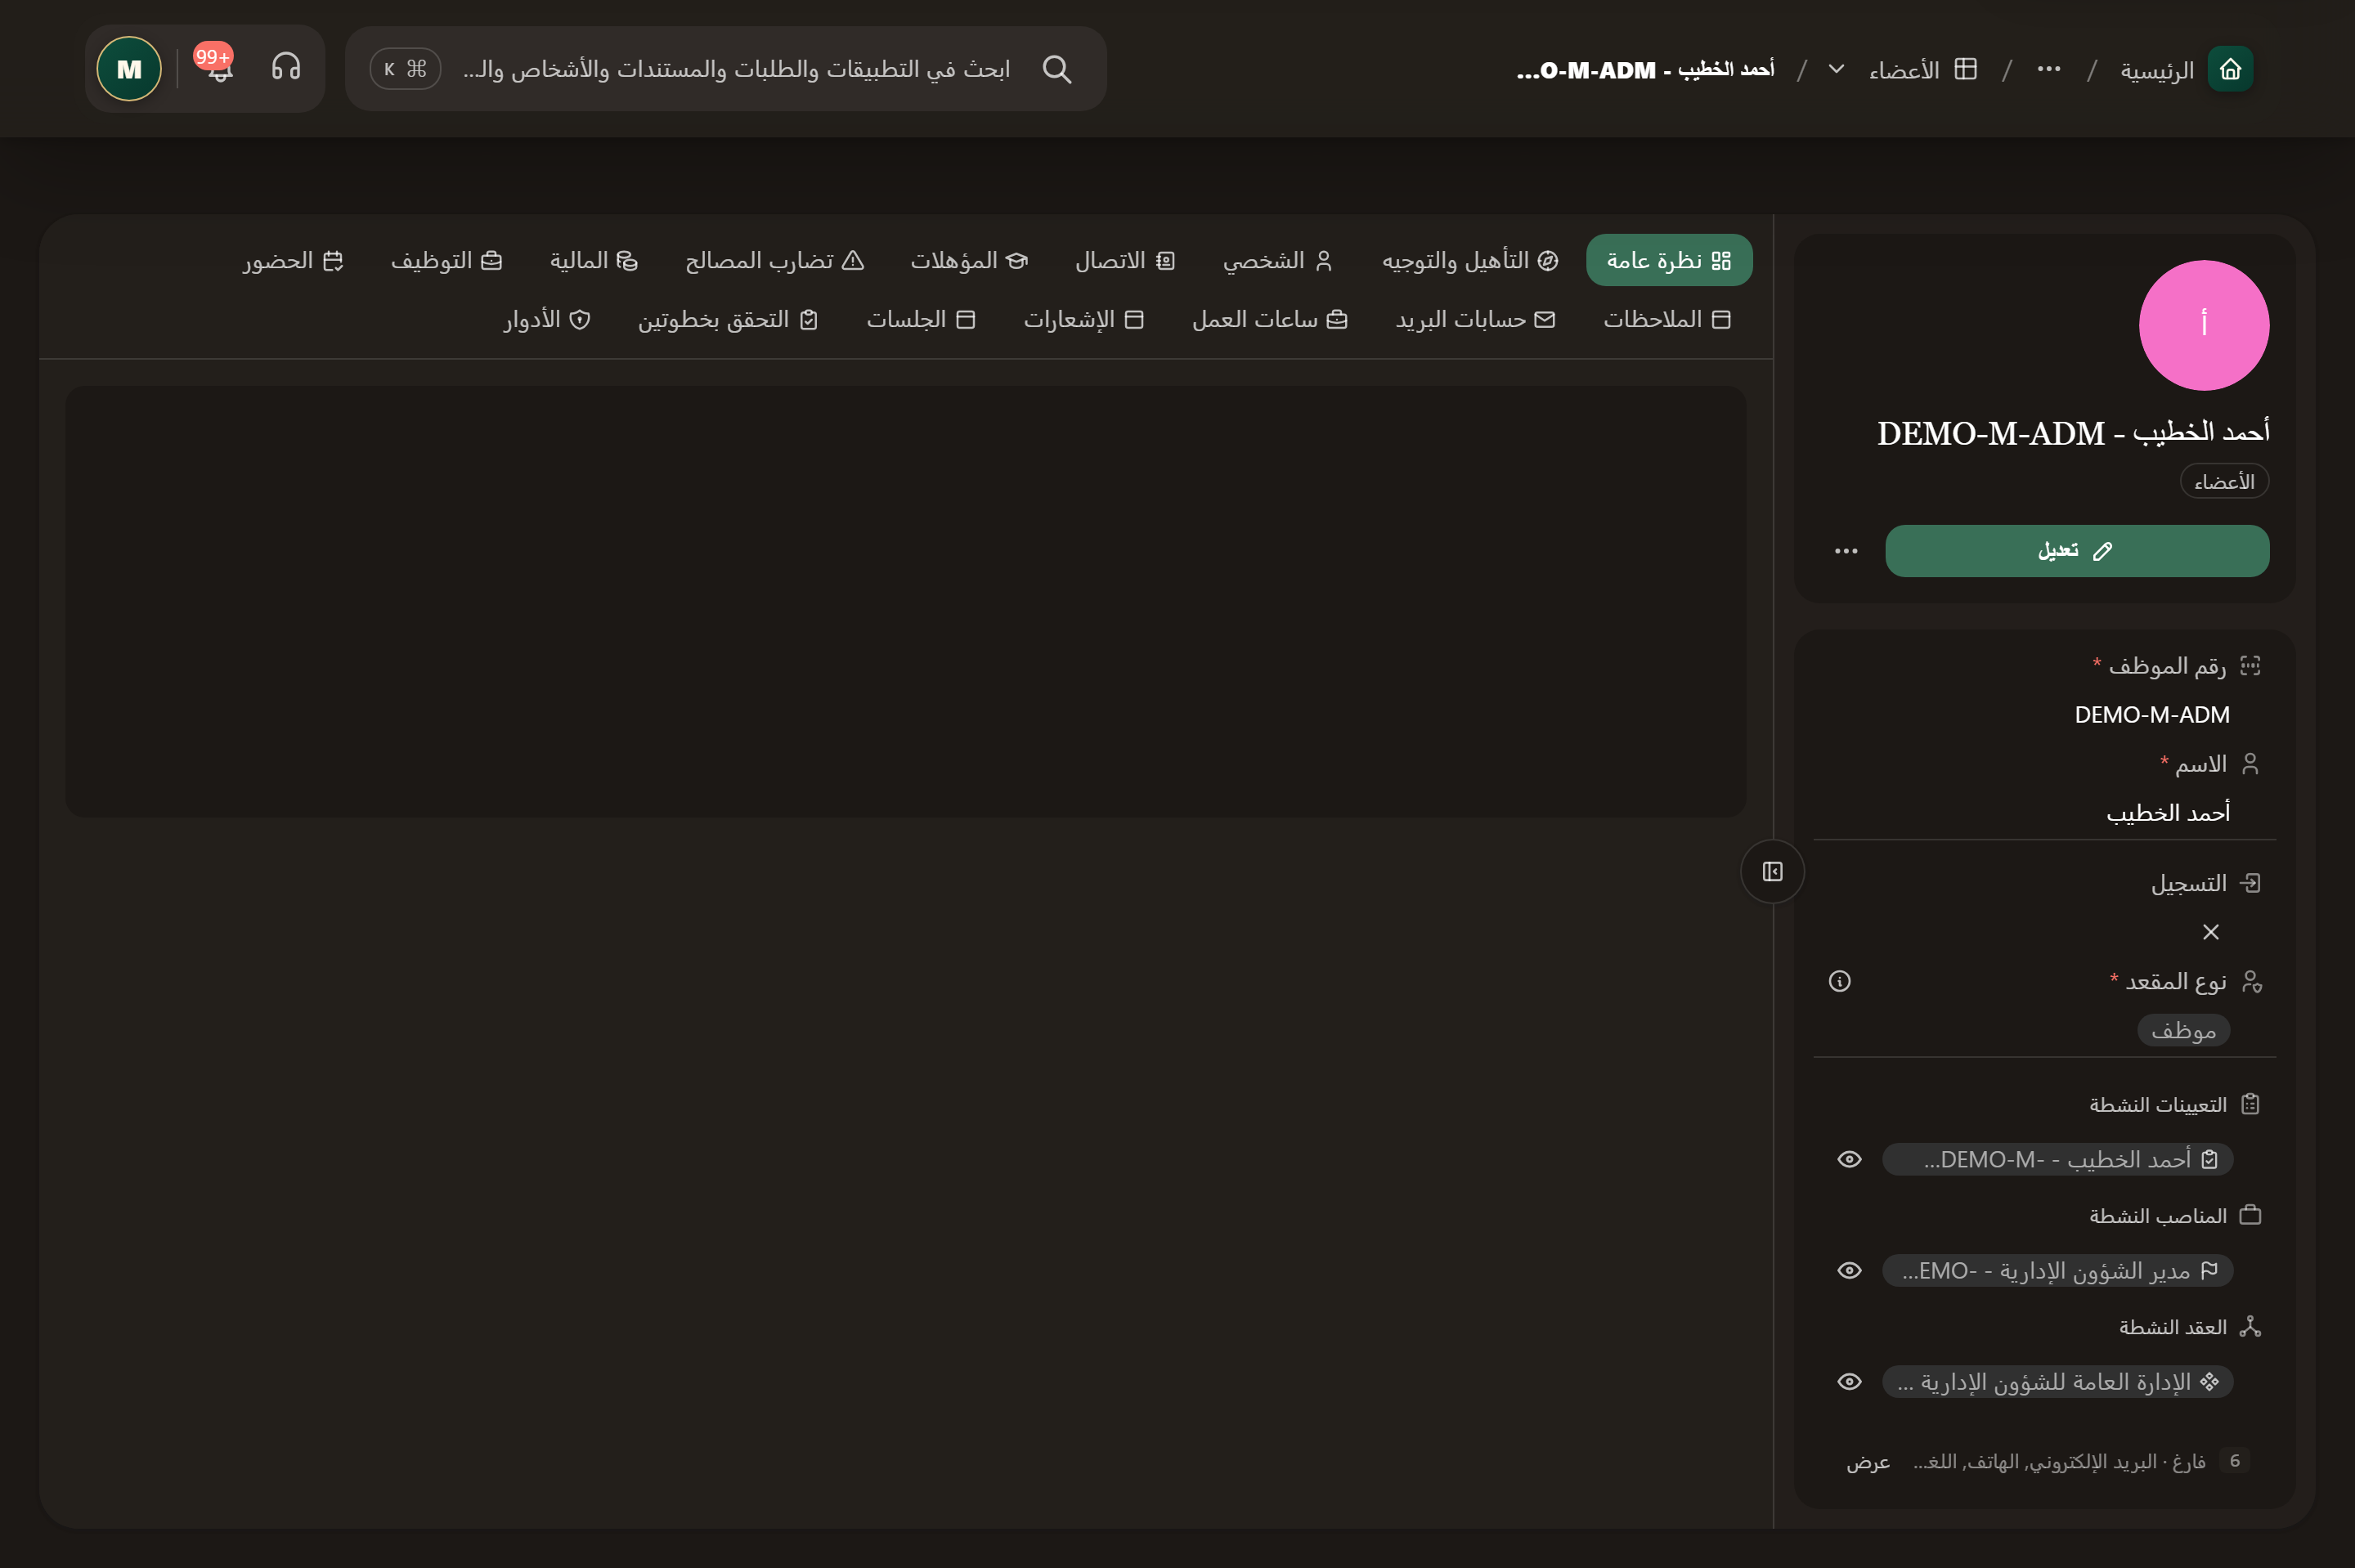
\includegraphics[width=0.95\linewidth]{figures/screens/ch02-member-fields-ar.png}
\caption{الأعضاء: ملف موظف تجريبي؛ يختلف عن مثال سارة}
\label{fig:hr-feature-members-screen}
\end{figure}

\begin{table}[H]
\centering
\caption{ما الذي تسجله في ملف العضو؟}
\label{tab:hr-feature-members-data}
\rcZebra
\begin{tabularx}{\linewidth}{R{3.6cm} Y}
\rcHeaderRow
\thh{التبويب أو القسم} & \thh{ما الذي تضيفه؟}\\
البيانات الرئيسية & رقم الموظف \req{} والاسم \req{}، والبريد والهاتف والصورة، و«التسجيل» (السماح بالدخول)، واللغة المفضلة والمنطقة الزمنية، ورقم البصمة.\\
الشخصي & اسم الأب واسم الأم، والجنس، والحالة الاجتماعية، وزمرة الدم، وتاريخ الميلاد ومكانه، والجنسية، والرقم الوطني وملفه، والسيرة الذاتية، وجواز السفر، ورخصة القيادة، ومعلومات العائلة.\\
الاتصال & العنوان وسند الإقامة، وأرقام الهاتف الشخصي والعمل والمنزل، والبريد الشخصي وبريد العمل، وجهات اتصال الطوارئ.\\
المؤهلات & التعليم، والمهارات ومستوى إتقانها، واللغات، والتدريبات، والخبرات السابقة؛ مع شهاداتها.\\
تضارب المصالح & الأقارب في المؤسسة، وجهة عمل أخرى، والتضارب مع الموردين أو الشركاء؛ مع القرار المتخذ وحالته.\\
المالية & الحسابات البنكية، وتأمين الموظف، والمكافآت والخصومات، وكشوف الرواتب.\\
التوظيف والحضور & تعيينات العضو، ورصيد إجازاته وسجل إجازاته.\\
تبويبات الحساب & حسابات البريد، والإشعارات وساعات الهدوء، والجلسات، والتحقق بخطوتين، والأجهزة المرتبطة (إن كانت الميزة مفعّلة).\\
\end{tabularx}
\end{table}

هذه هي الحقول الافتراضية، وقد يعدّلها مسؤول مؤسستك. يملأ النظام حقلي المناصب والوحدات النشطة \gen{} من التعيينات.

\subsection{ما الذي يمكنك فعله؟}

\begin{itemize}
  \item «إضافة تعيين» من ملف العضو؛ يظهر فيه العضو مختاراً مسبقاً.
  \item «تغيير كلمة المرور»، مع خيار إلزامه بتغييرها عند دخوله التالي.
  \item «إنهاء ارتباط العضو»: اختر لمسؤولياته «نقل» إلى موظف بديل أو «إلغاء إسناد» أو «الإبقاء»، وحدد تاريخ السريان، وراجع ما سيتأثر.
  \item في القائمة بطاقات تعرض إجمالي الأعضاء، ومن لديهم تعيينات نشطة، ومن ليست لديهم.
\end{itemize}

\begin{figure}[H]
\centering
\begin{tikzpicture}[node distance=0.5cm,stepBox/.append style={minimum width=6.5cm,text width=6.1cm,minimum height=0.8cm}]
  \node[stepBox] (a) {\RL{إنشاء سجل سارة}};
  \node[stepBox,below=of a] (b) {\RL{التعيين الوظيفي}};
  \node[stepBox,below=of b] (c) {\RL{مراجعة الوظيفة}\\\RL{والفترة}};
  \draw[flowsTo] (a) -- (b);
  \draw[flowsTo] (b) -- (c);
\end{tikzpicture}
\rclegend
\caption{خطوات الاستخدام؛ الأسهم لا تعني معالجة تلقائية}
\label{fig:hr-feature-members-flow}
\end{figure}

\subsection{جرّب وراجع}

\begin{enumerate}
  \item افتح «الأعضاء» وابحث عن سارة قبل إضافة سجل جديد، لتجنب التكرار.
  \item أضف رقم الموظف \en{0001} والاسم «سارة الخطيب» والبريد، ثم «حفظ».
  \item افتح تبويب «الاتصال» وأضف جهة اتصال طوارئ بالاسم والهاتف والعلاقة، ثم احفظ.
  \item من قائمة إجراءات السجل اختر «إضافة تعيين» واربطها بمنصبها.
\end{enumerate}

\textbf{تحقق:} أعد فتح السجل وراجع التبويبات. تظهر وظيفتها في تبويب «التوظيف» بعد حفظ التعيين.

\subsection{تبويبات ملف الموظف}

\begin{figure}[H]
\centering
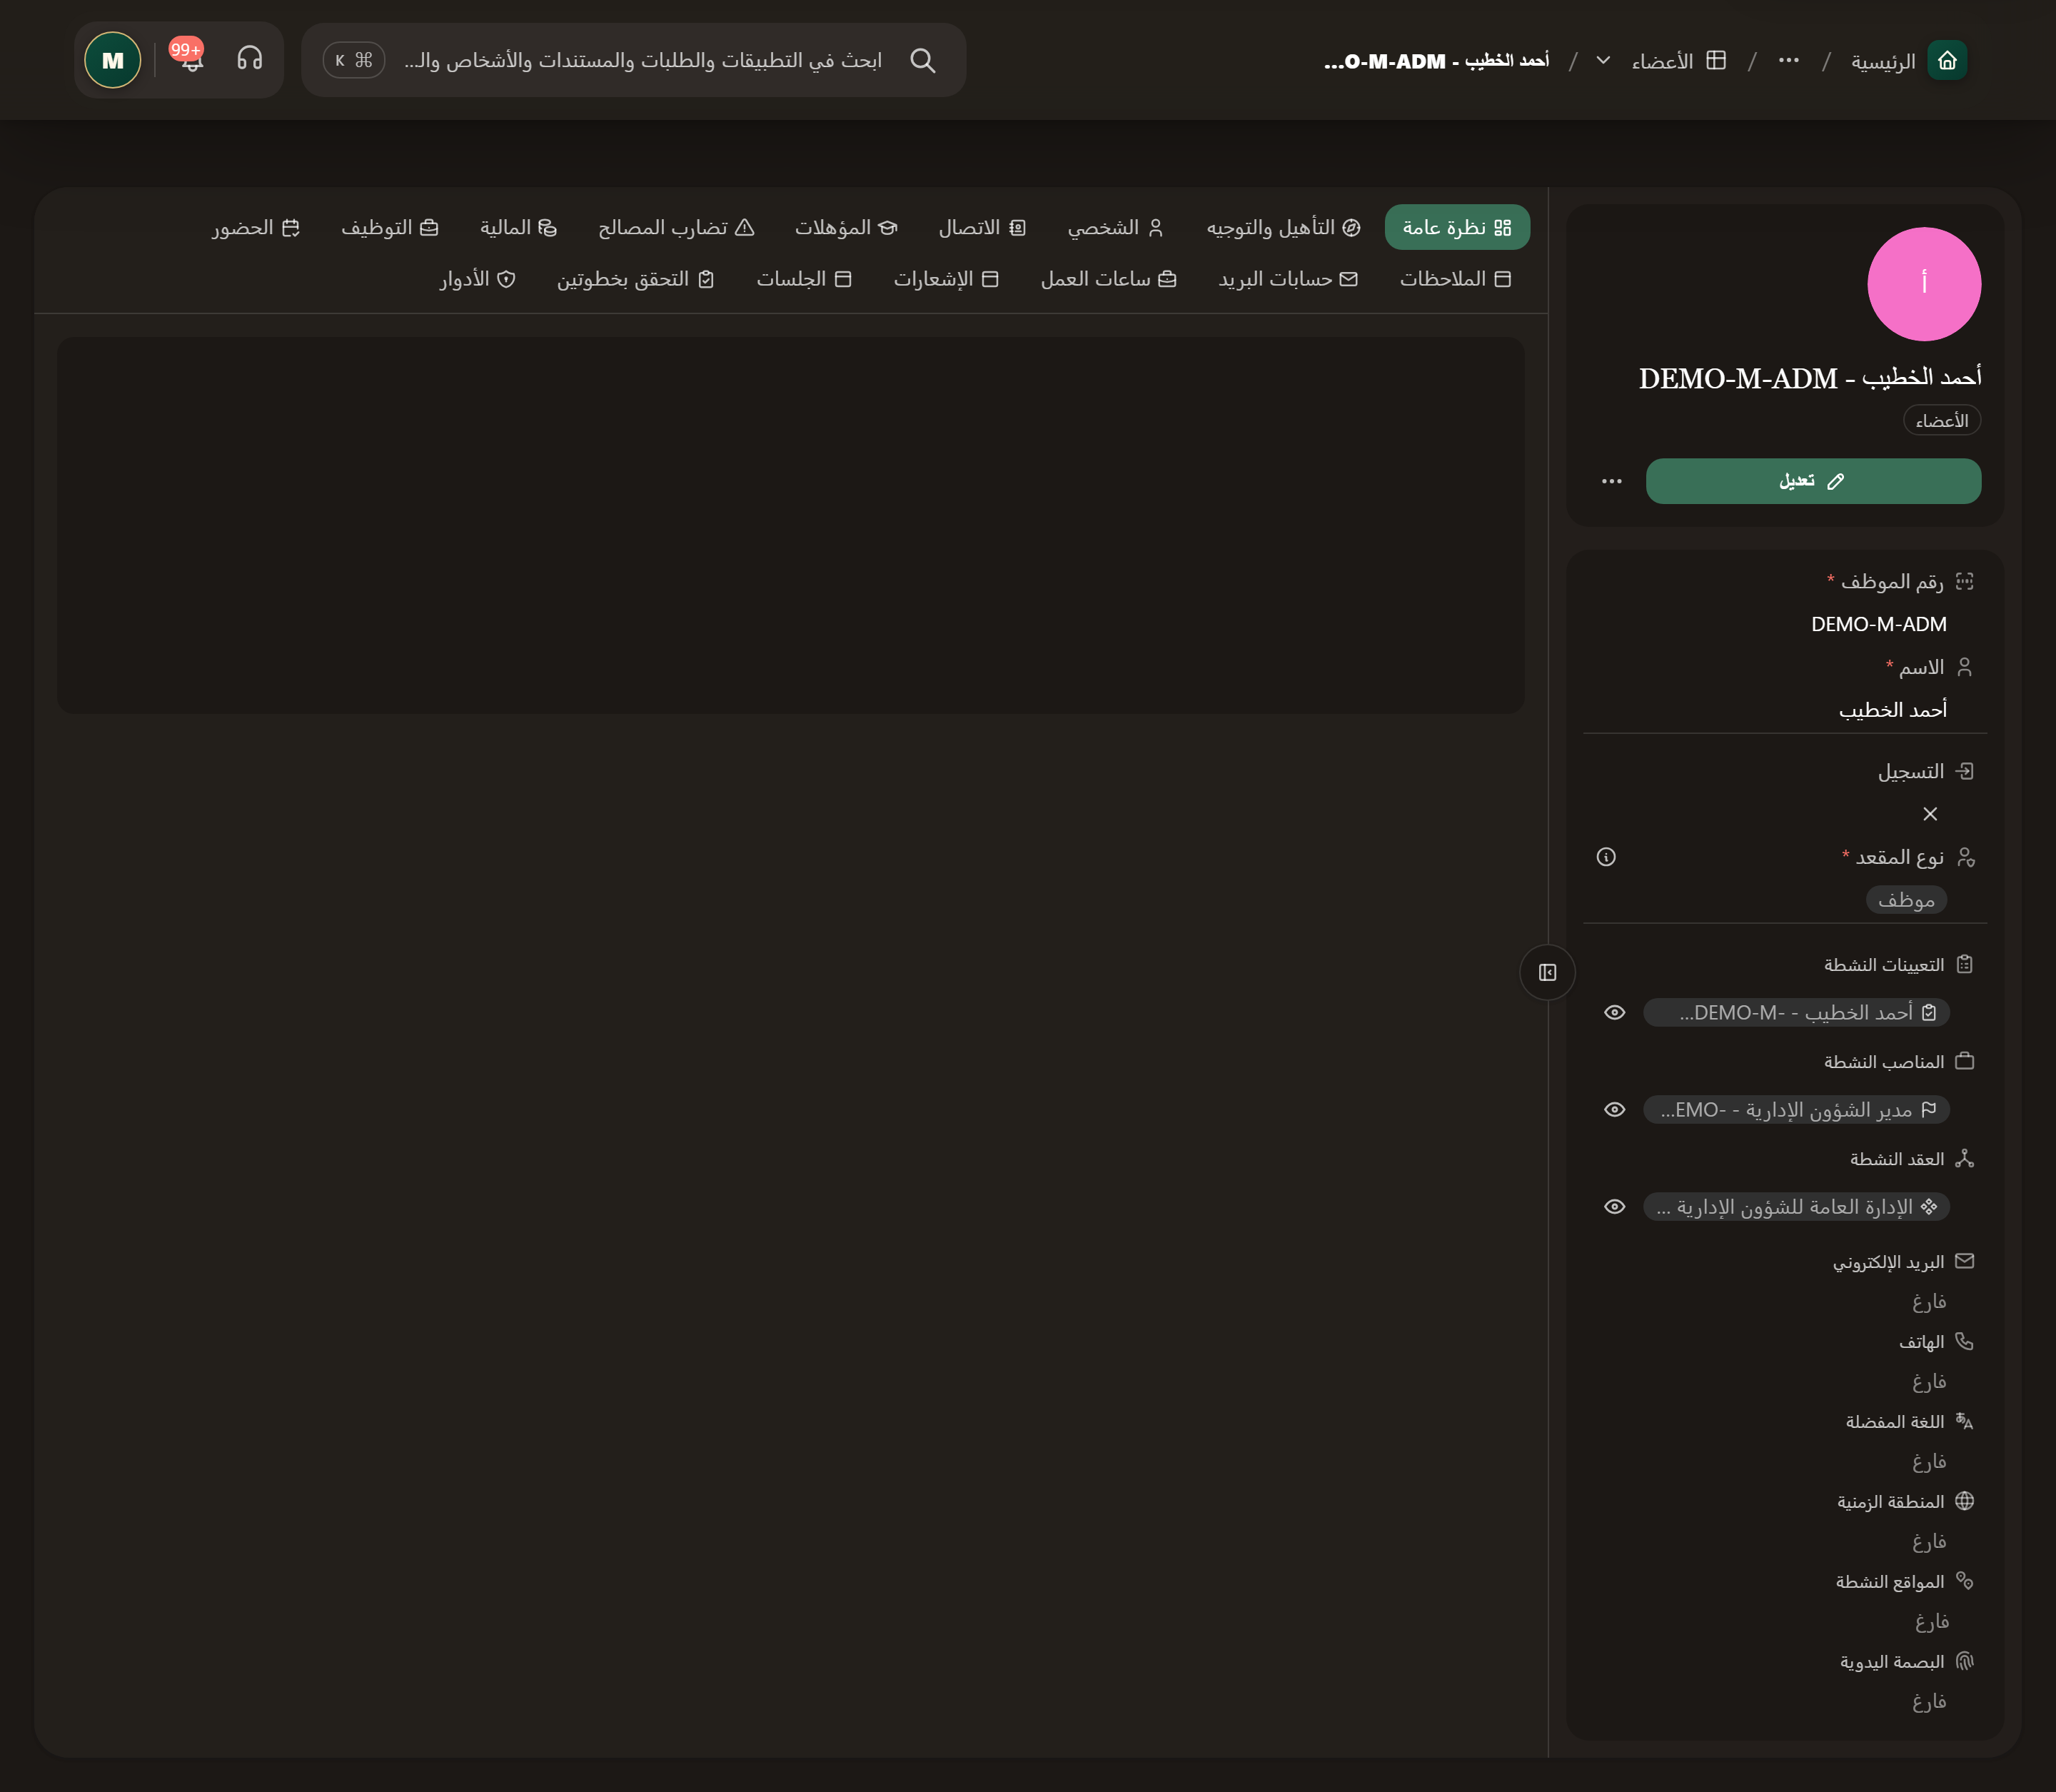
\includegraphics[width=0.95\linewidth]{figures/screens/ch03-member-tab1-ar.png}
\caption{ملف الموظف التجريبي — تبويب «نظرة عامة»}
\label{fig:hr-member-tab1}
\end{figure}

\begin{figure}[H]
\centering
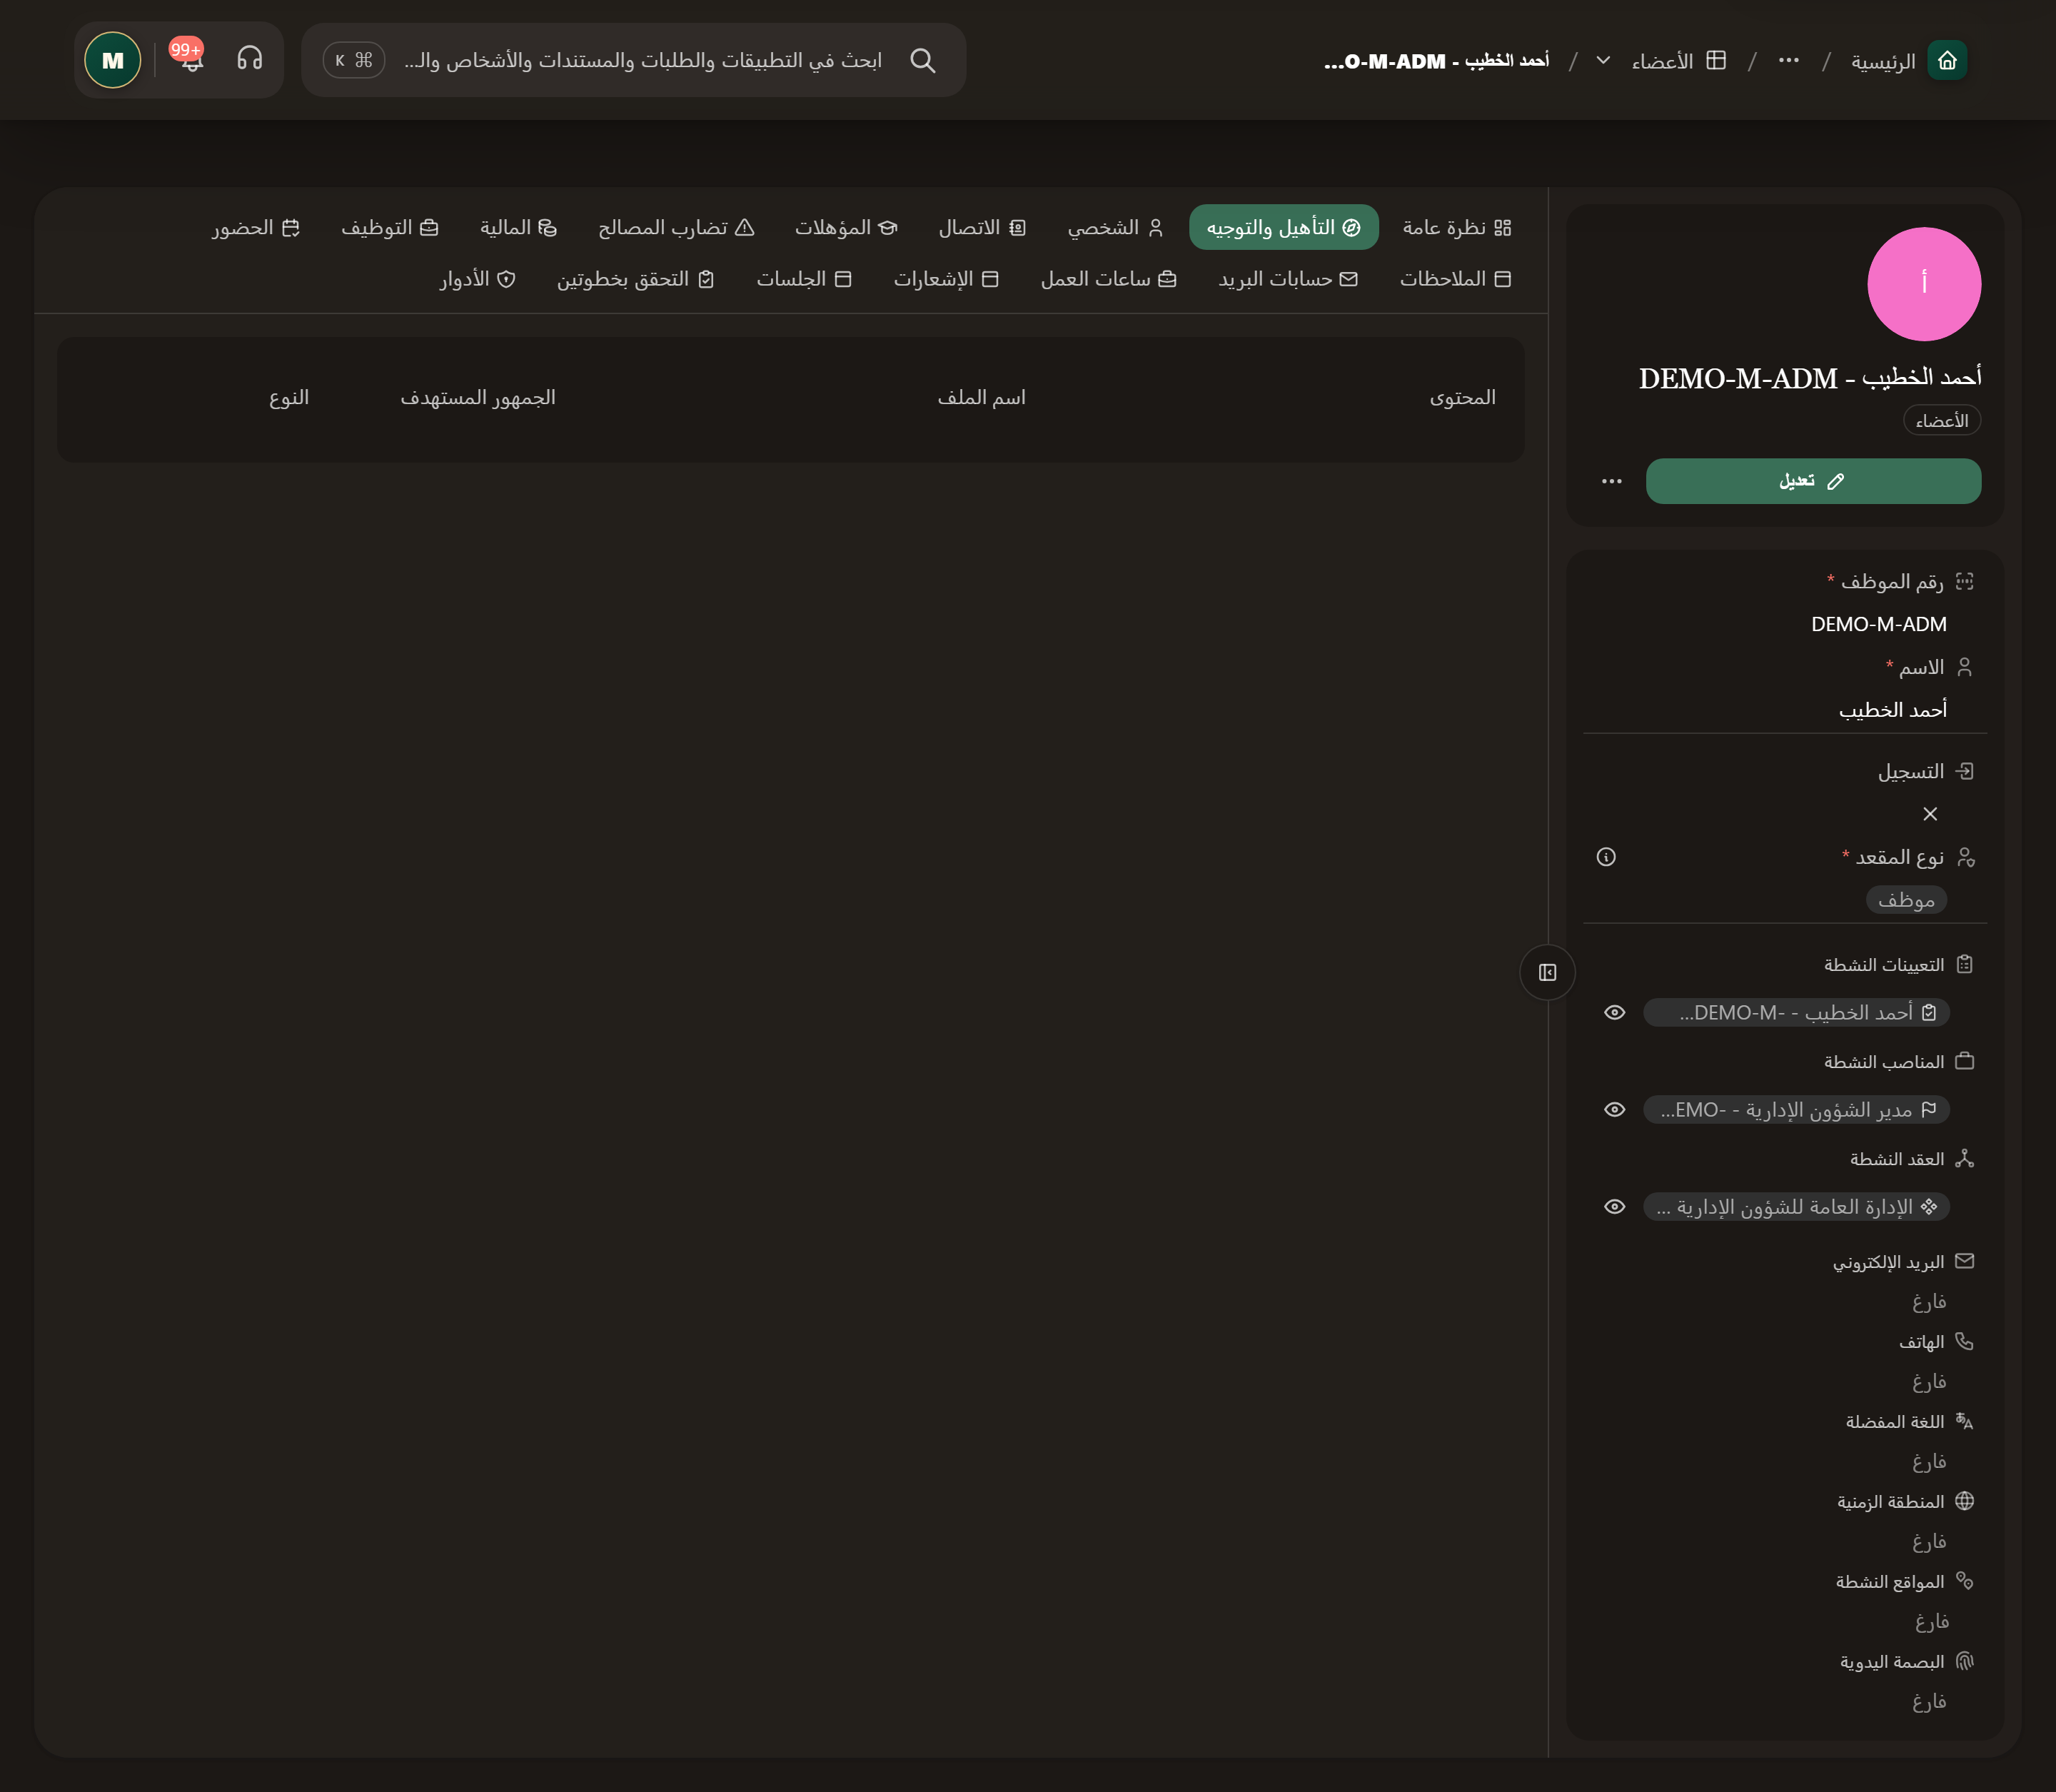
\includegraphics[width=0.95\linewidth]{figures/screens/ch03-member-tab2-ar.png}
\caption{ملف الموظف التجريبي — تبويب «التأهيل والتوجيه»}
\label{fig:hr-member-tab2}
\end{figure}

\begin{figure}[H]
\centering
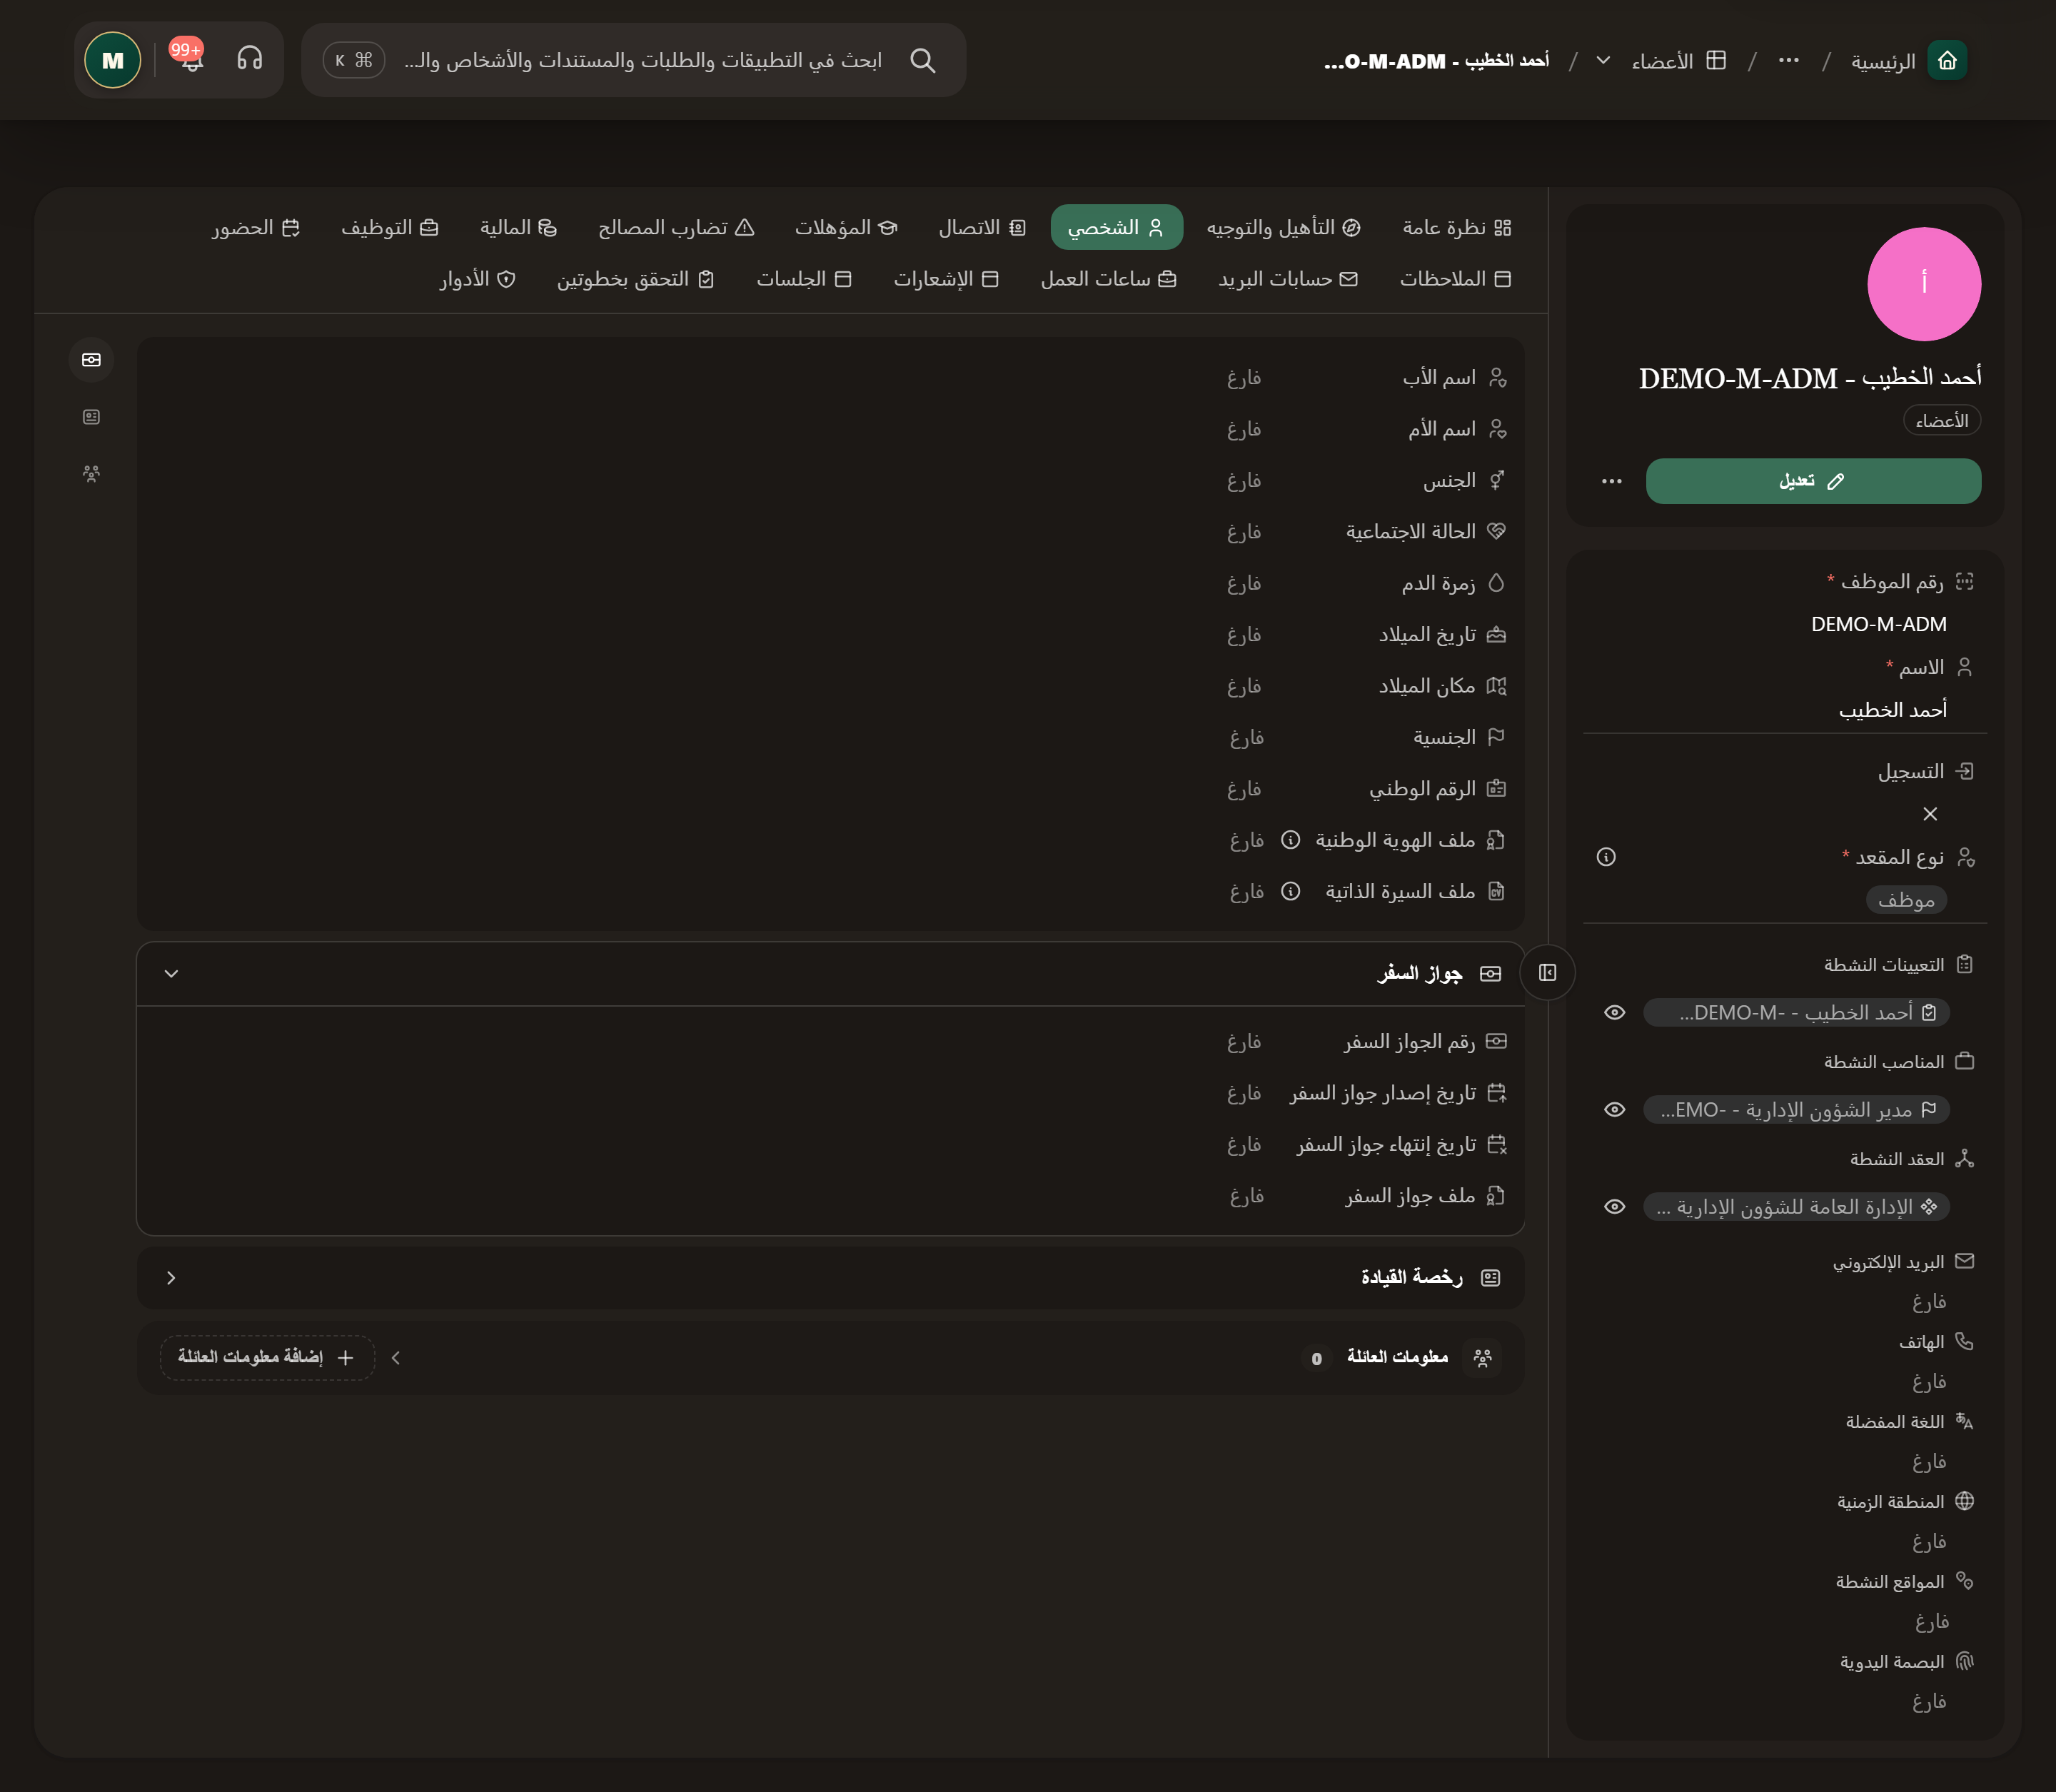
\includegraphics[width=0.95\linewidth]{figures/screens/ch03-member-tab3-ar.png}
\caption{ملف الموظف التجريبي — تبويب «الشخصي»}
\label{fig:hr-member-tab3}
\end{figure}

\begin{figure}[H]
\centering
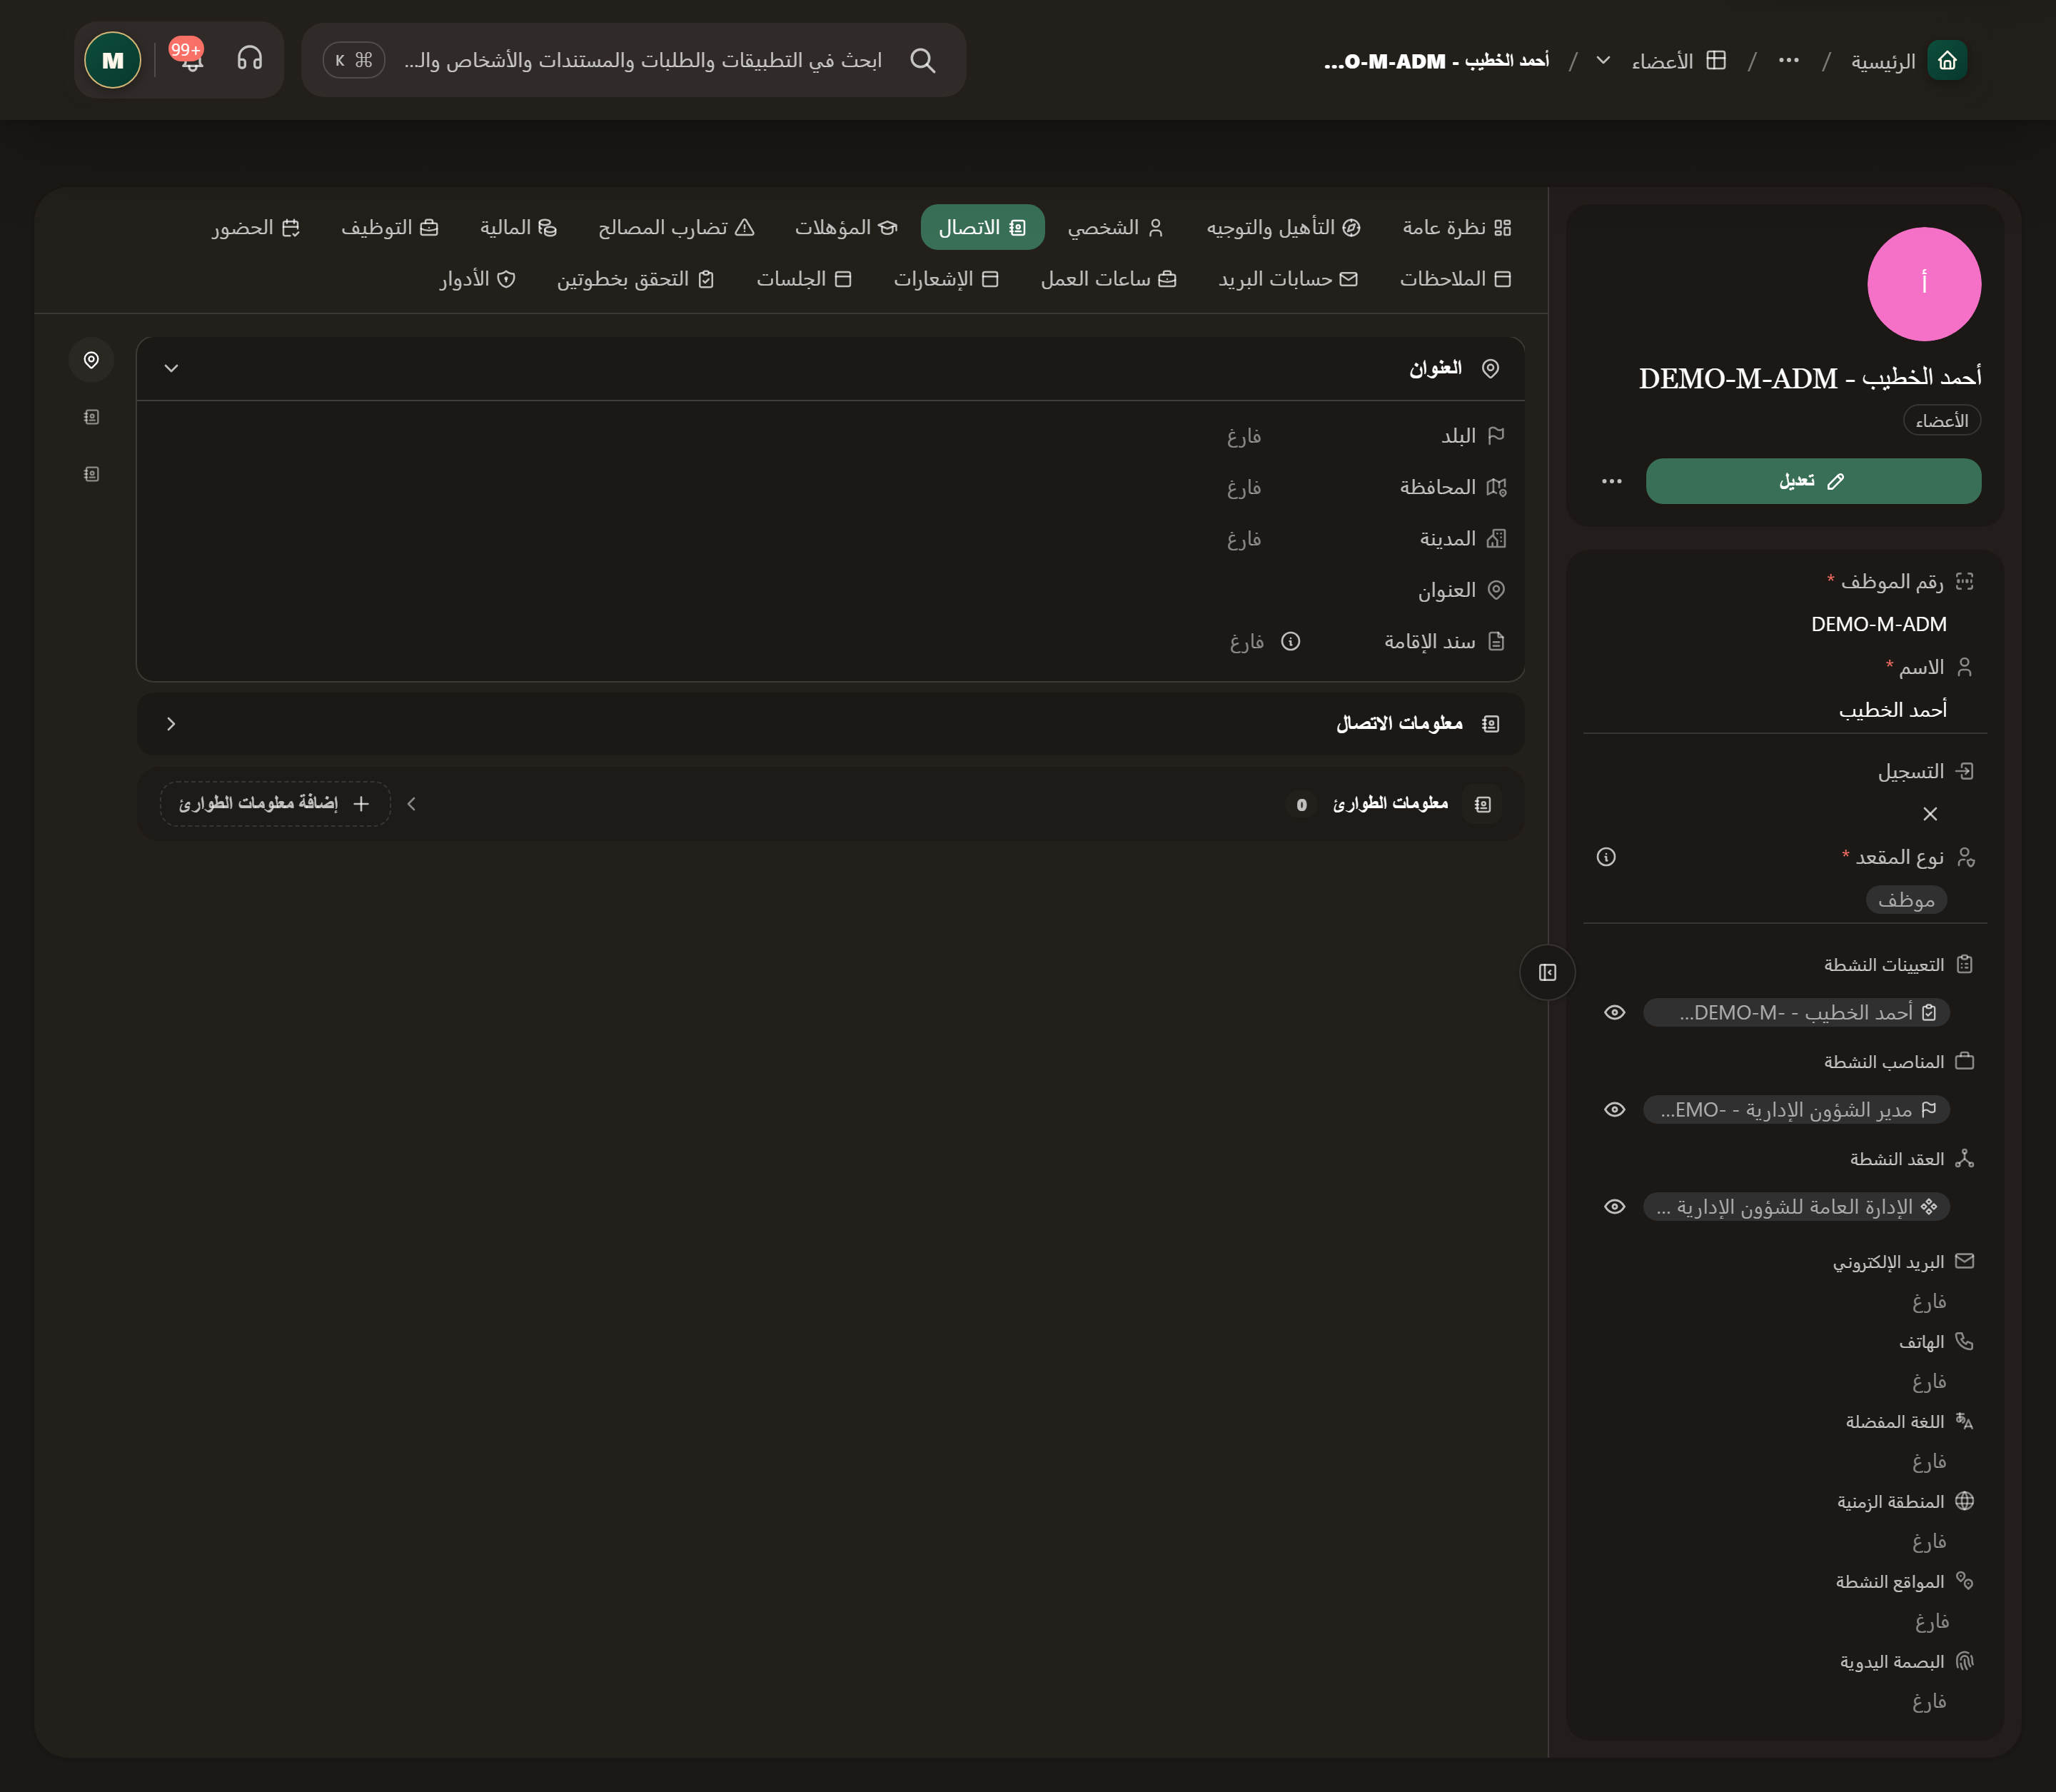
\includegraphics[width=0.95\linewidth]{figures/screens/ch03-member-tab4-ar.png}
\caption{ملف الموظف التجريبي — تبويب «الاتصال»}
\label{fig:hr-member-tab4}
\end{figure}

\begin{figure}[H]
\centering
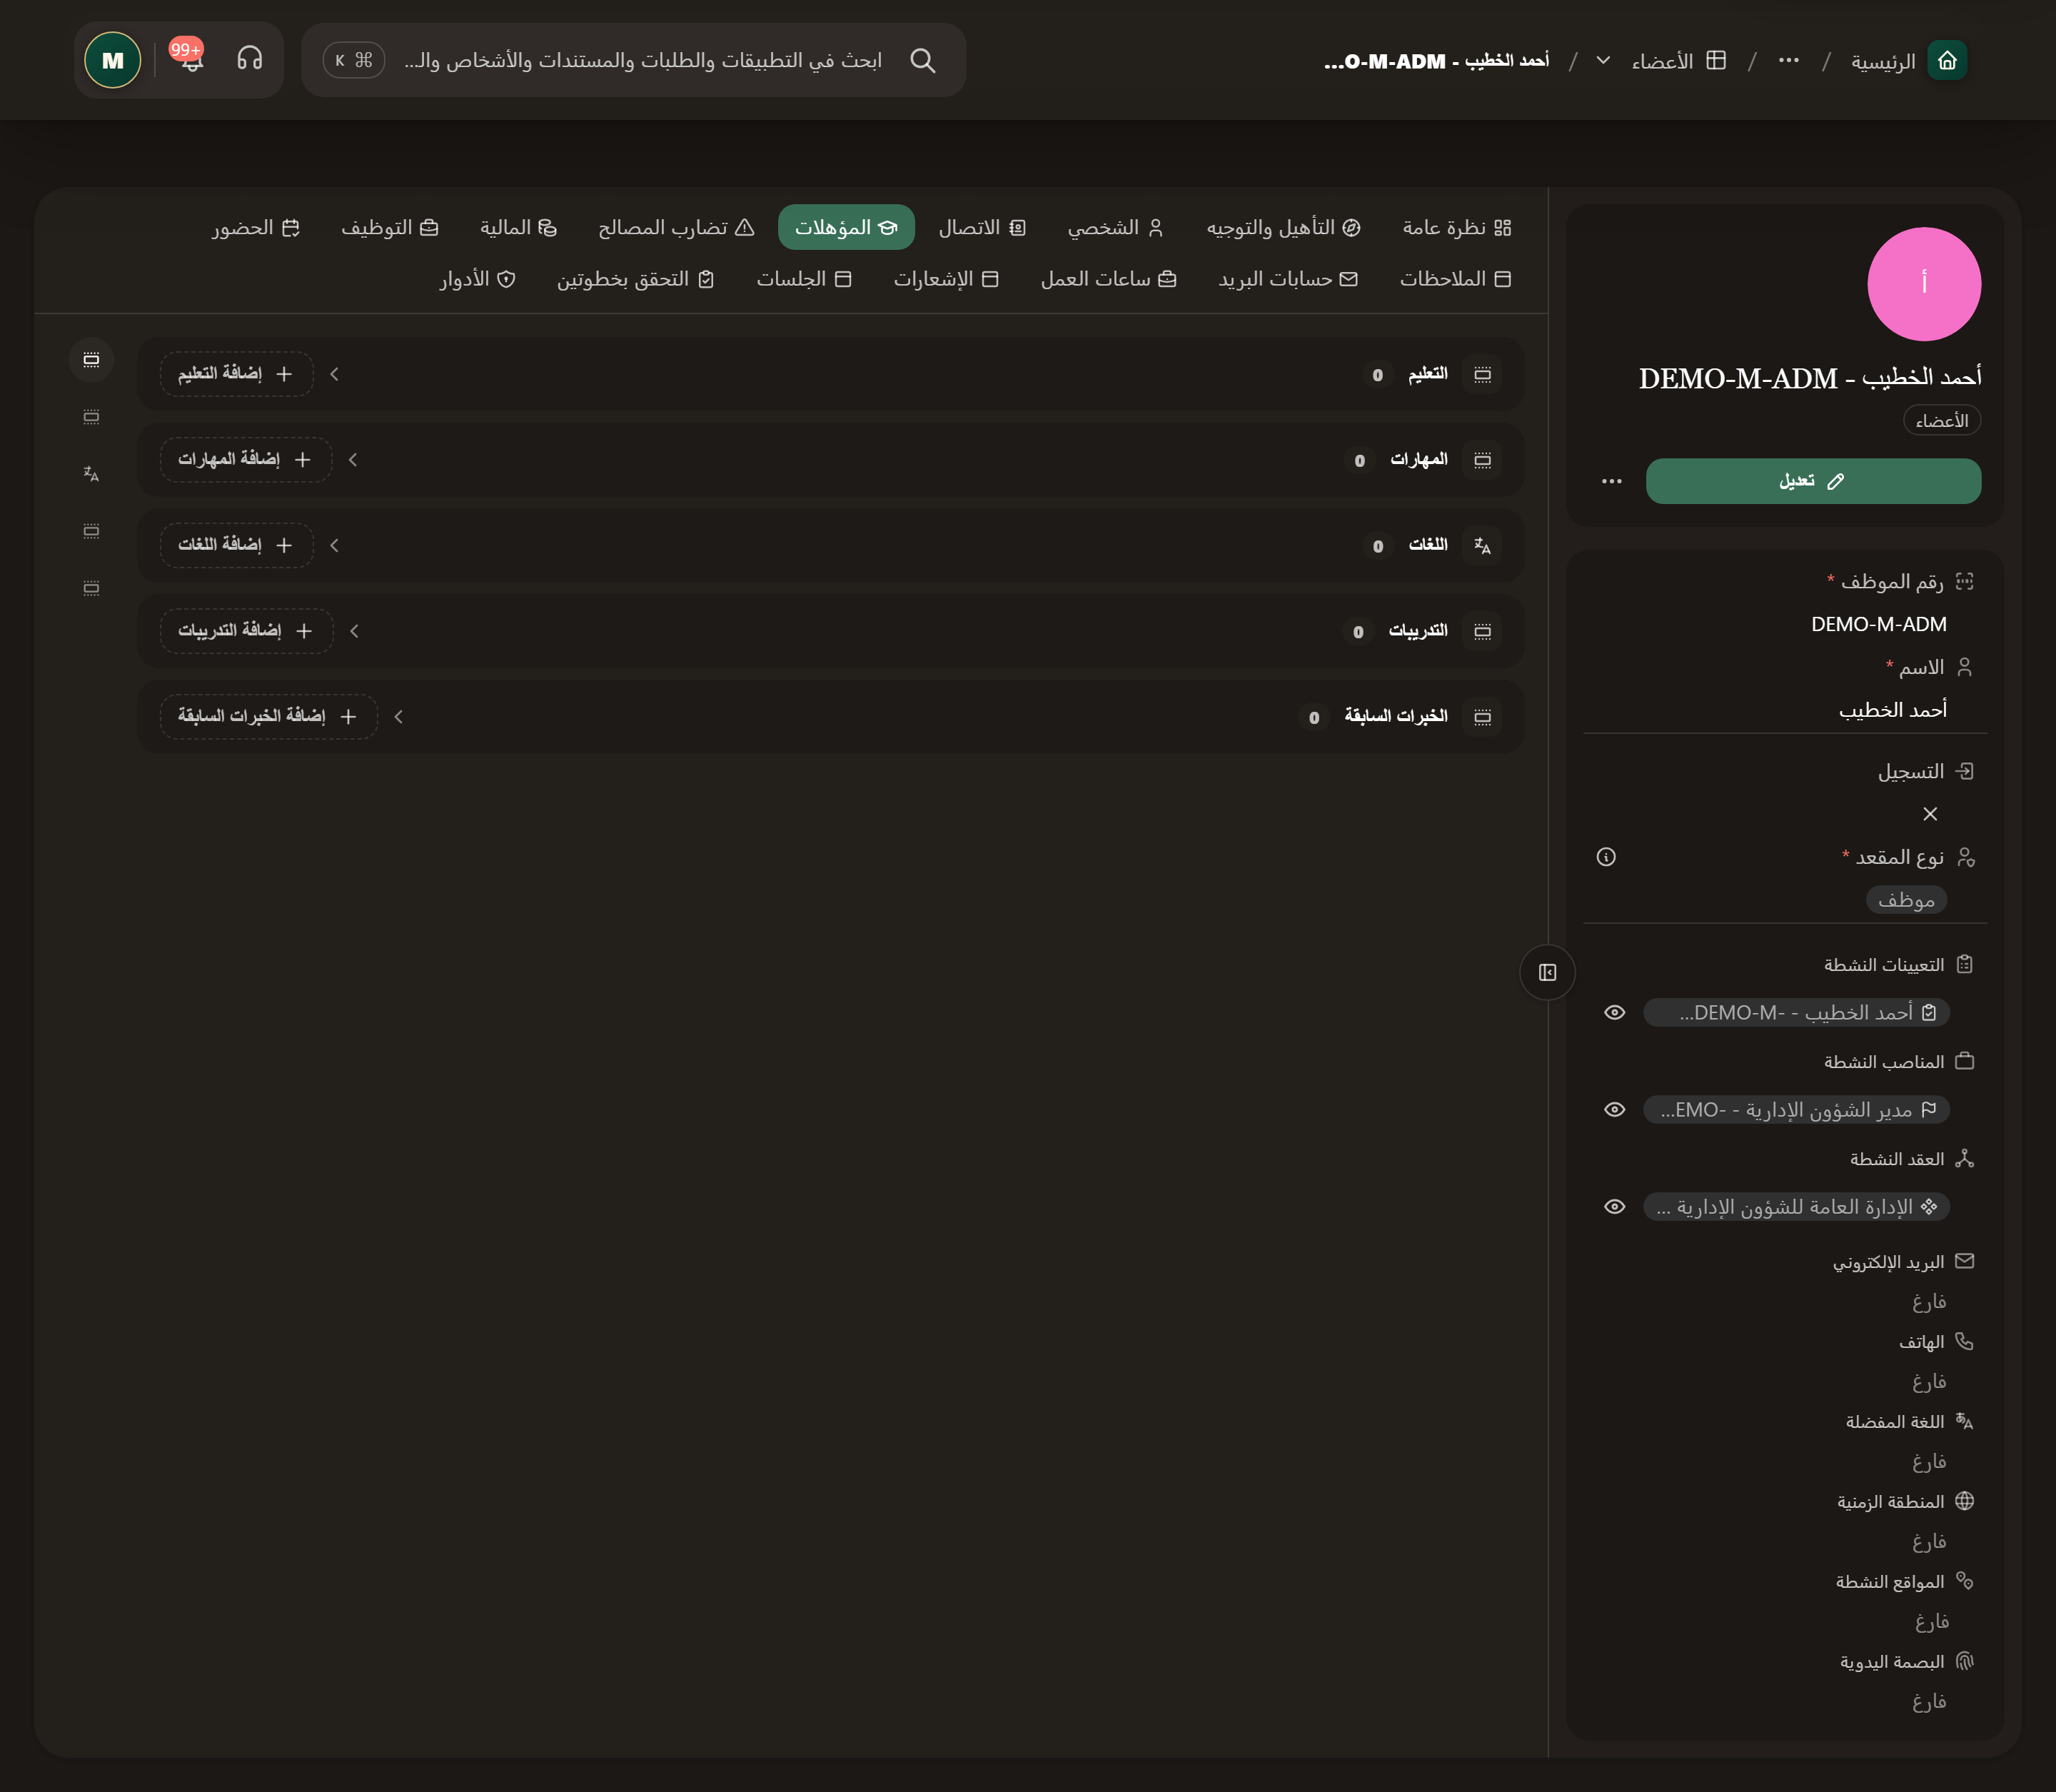
\includegraphics[width=0.95\linewidth]{figures/screens/ch03-member-tab5-ar.png}
\caption{ملف الموظف التجريبي — تبويب «المؤهلات»}
\label{fig:hr-member-tab5}
\end{figure}

\begin{figure}[H]
\centering
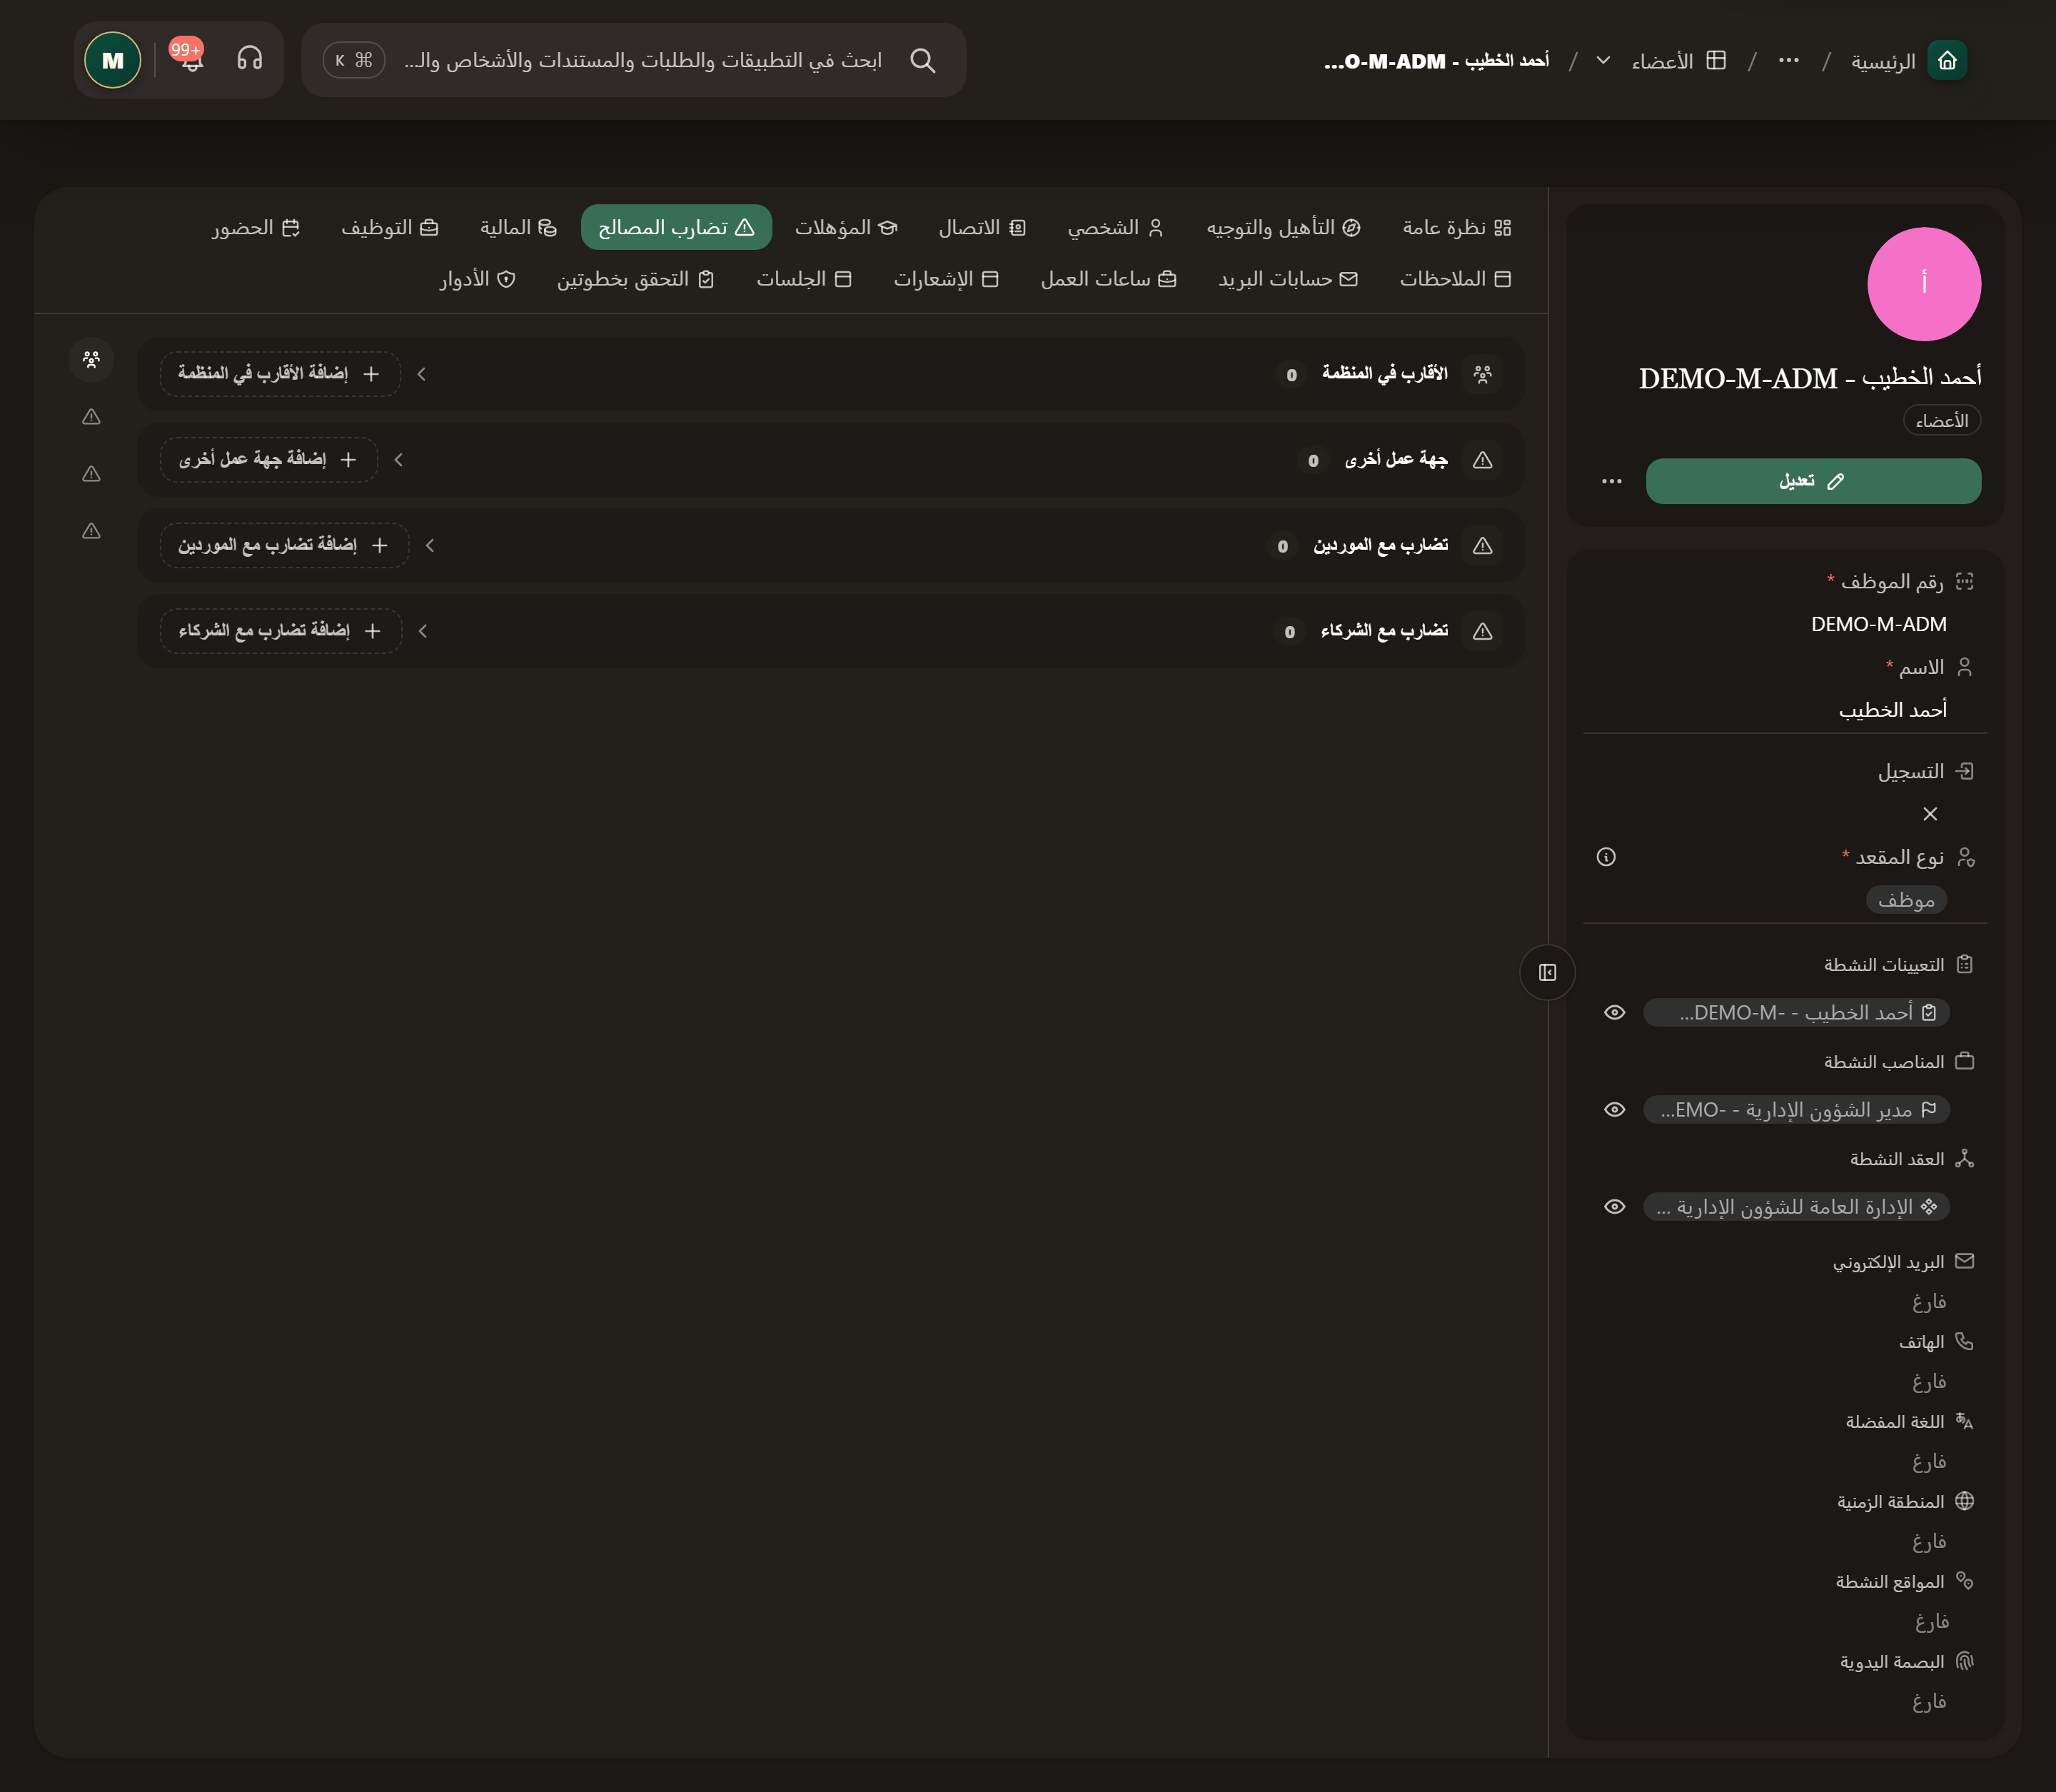
\includegraphics[width=0.95\linewidth]{figures/screens/ch03-member-tab6-ar.png}
\caption{ملف الموظف التجريبي — تبويب «تضارب المصالح»}
\label{fig:hr-member-tab6}
\end{figure}

\begin{figure}[H]
\centering
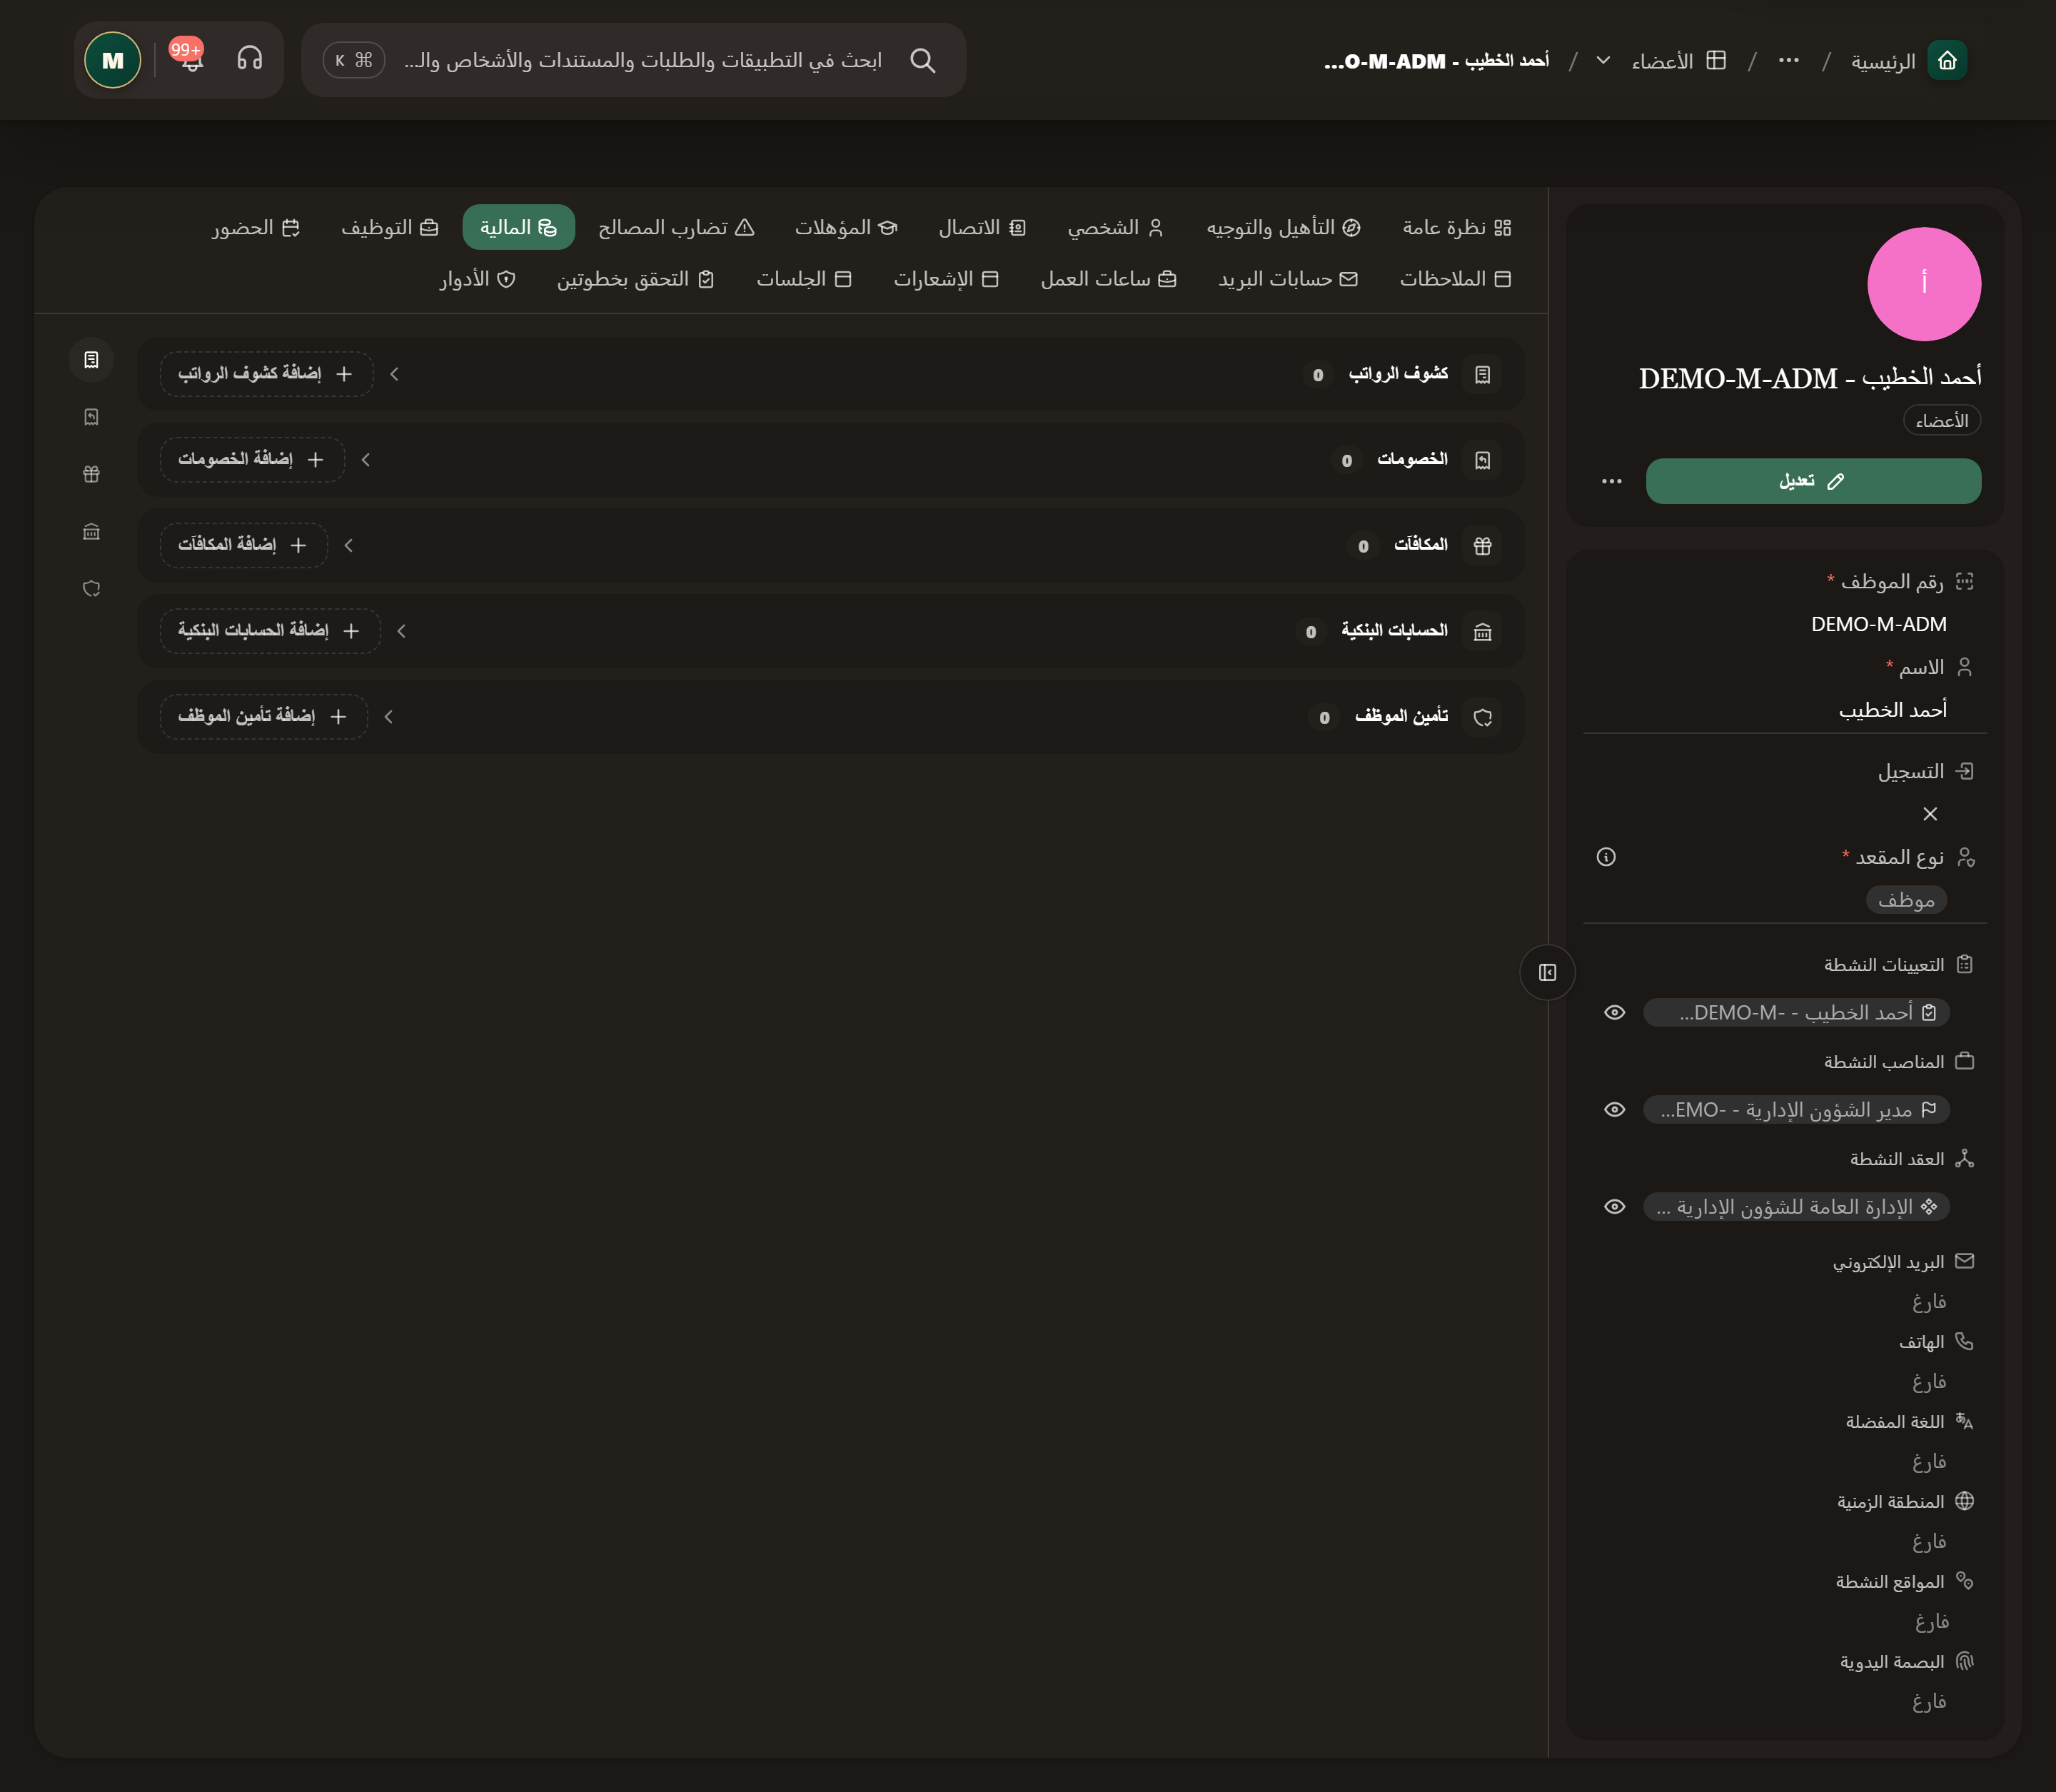
\includegraphics[width=0.95\linewidth]{figures/screens/ch03-member-tab7-ar.png}
\caption{ملف الموظف التجريبي — تبويب «المالية»}
\label{fig:hr-member-tab7}
\end{figure}

\begin{figure}[H]
\centering
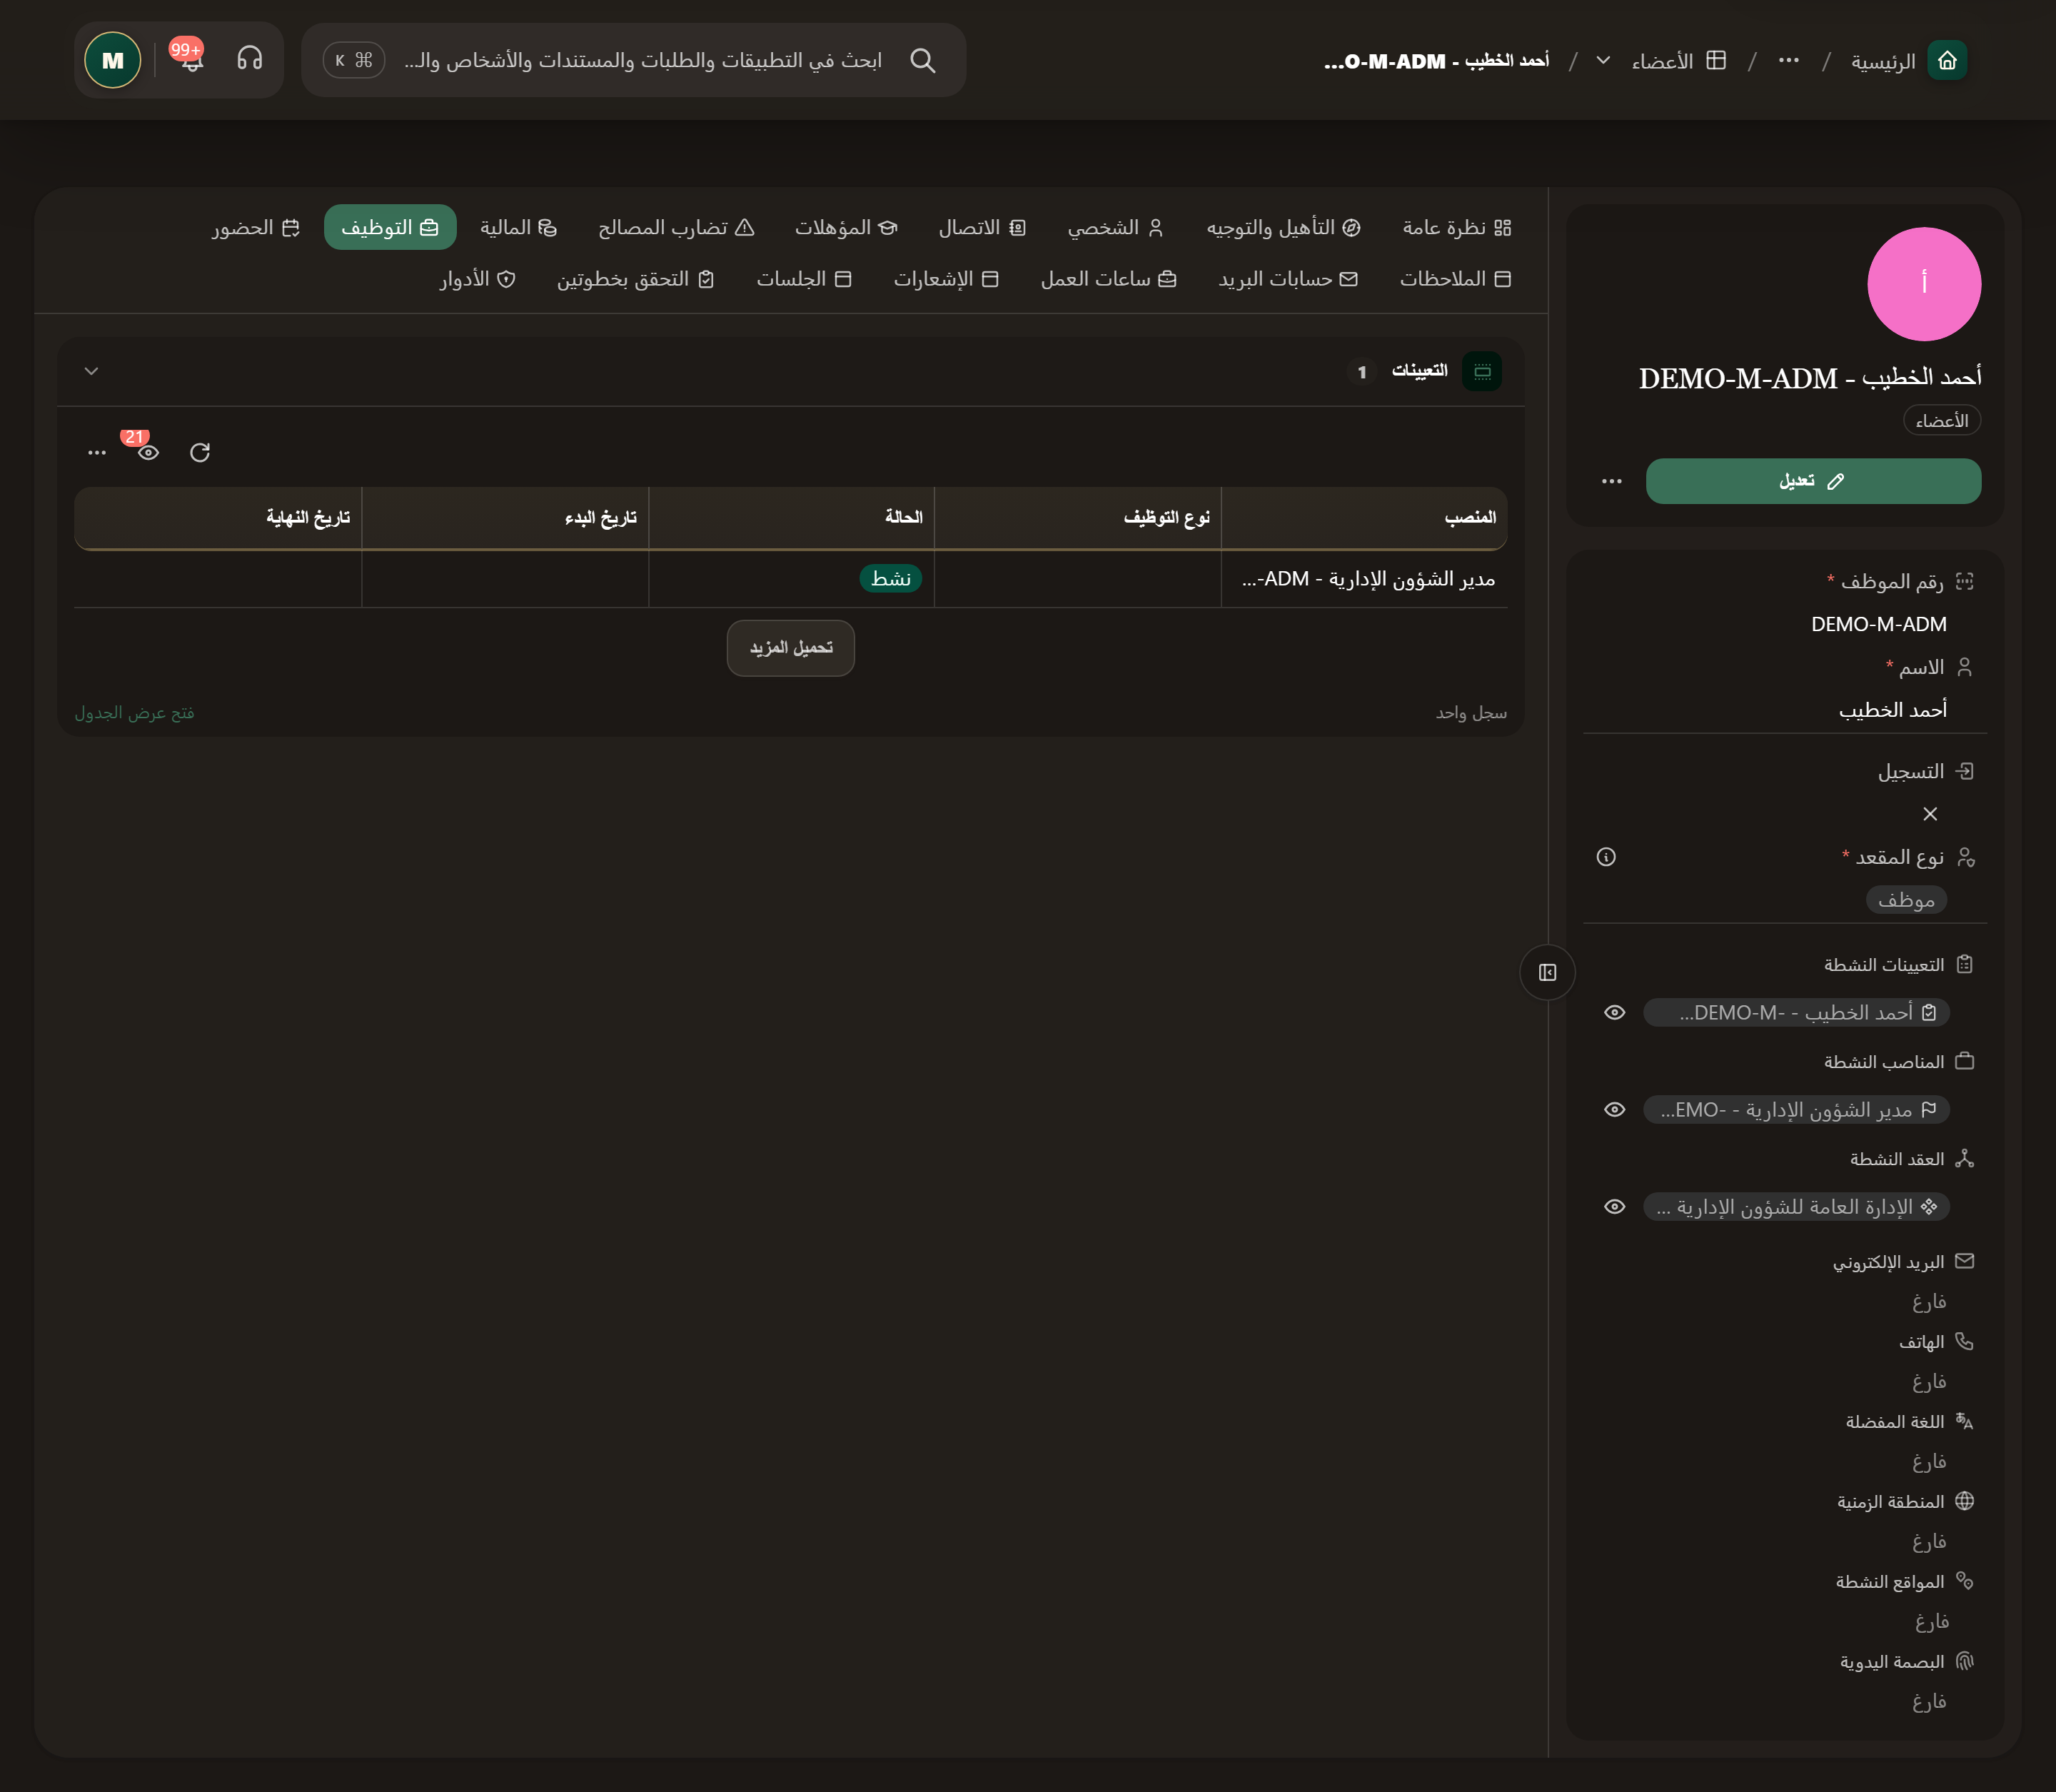
\includegraphics[width=0.95\linewidth]{figures/screens/ch03-member-tab8-ar.png}
\caption{ملف الموظف التجريبي — تبويب «التوظيف»}
\label{fig:hr-member-tab8}
\end{figure}

\begin{figure}[H]
\centering
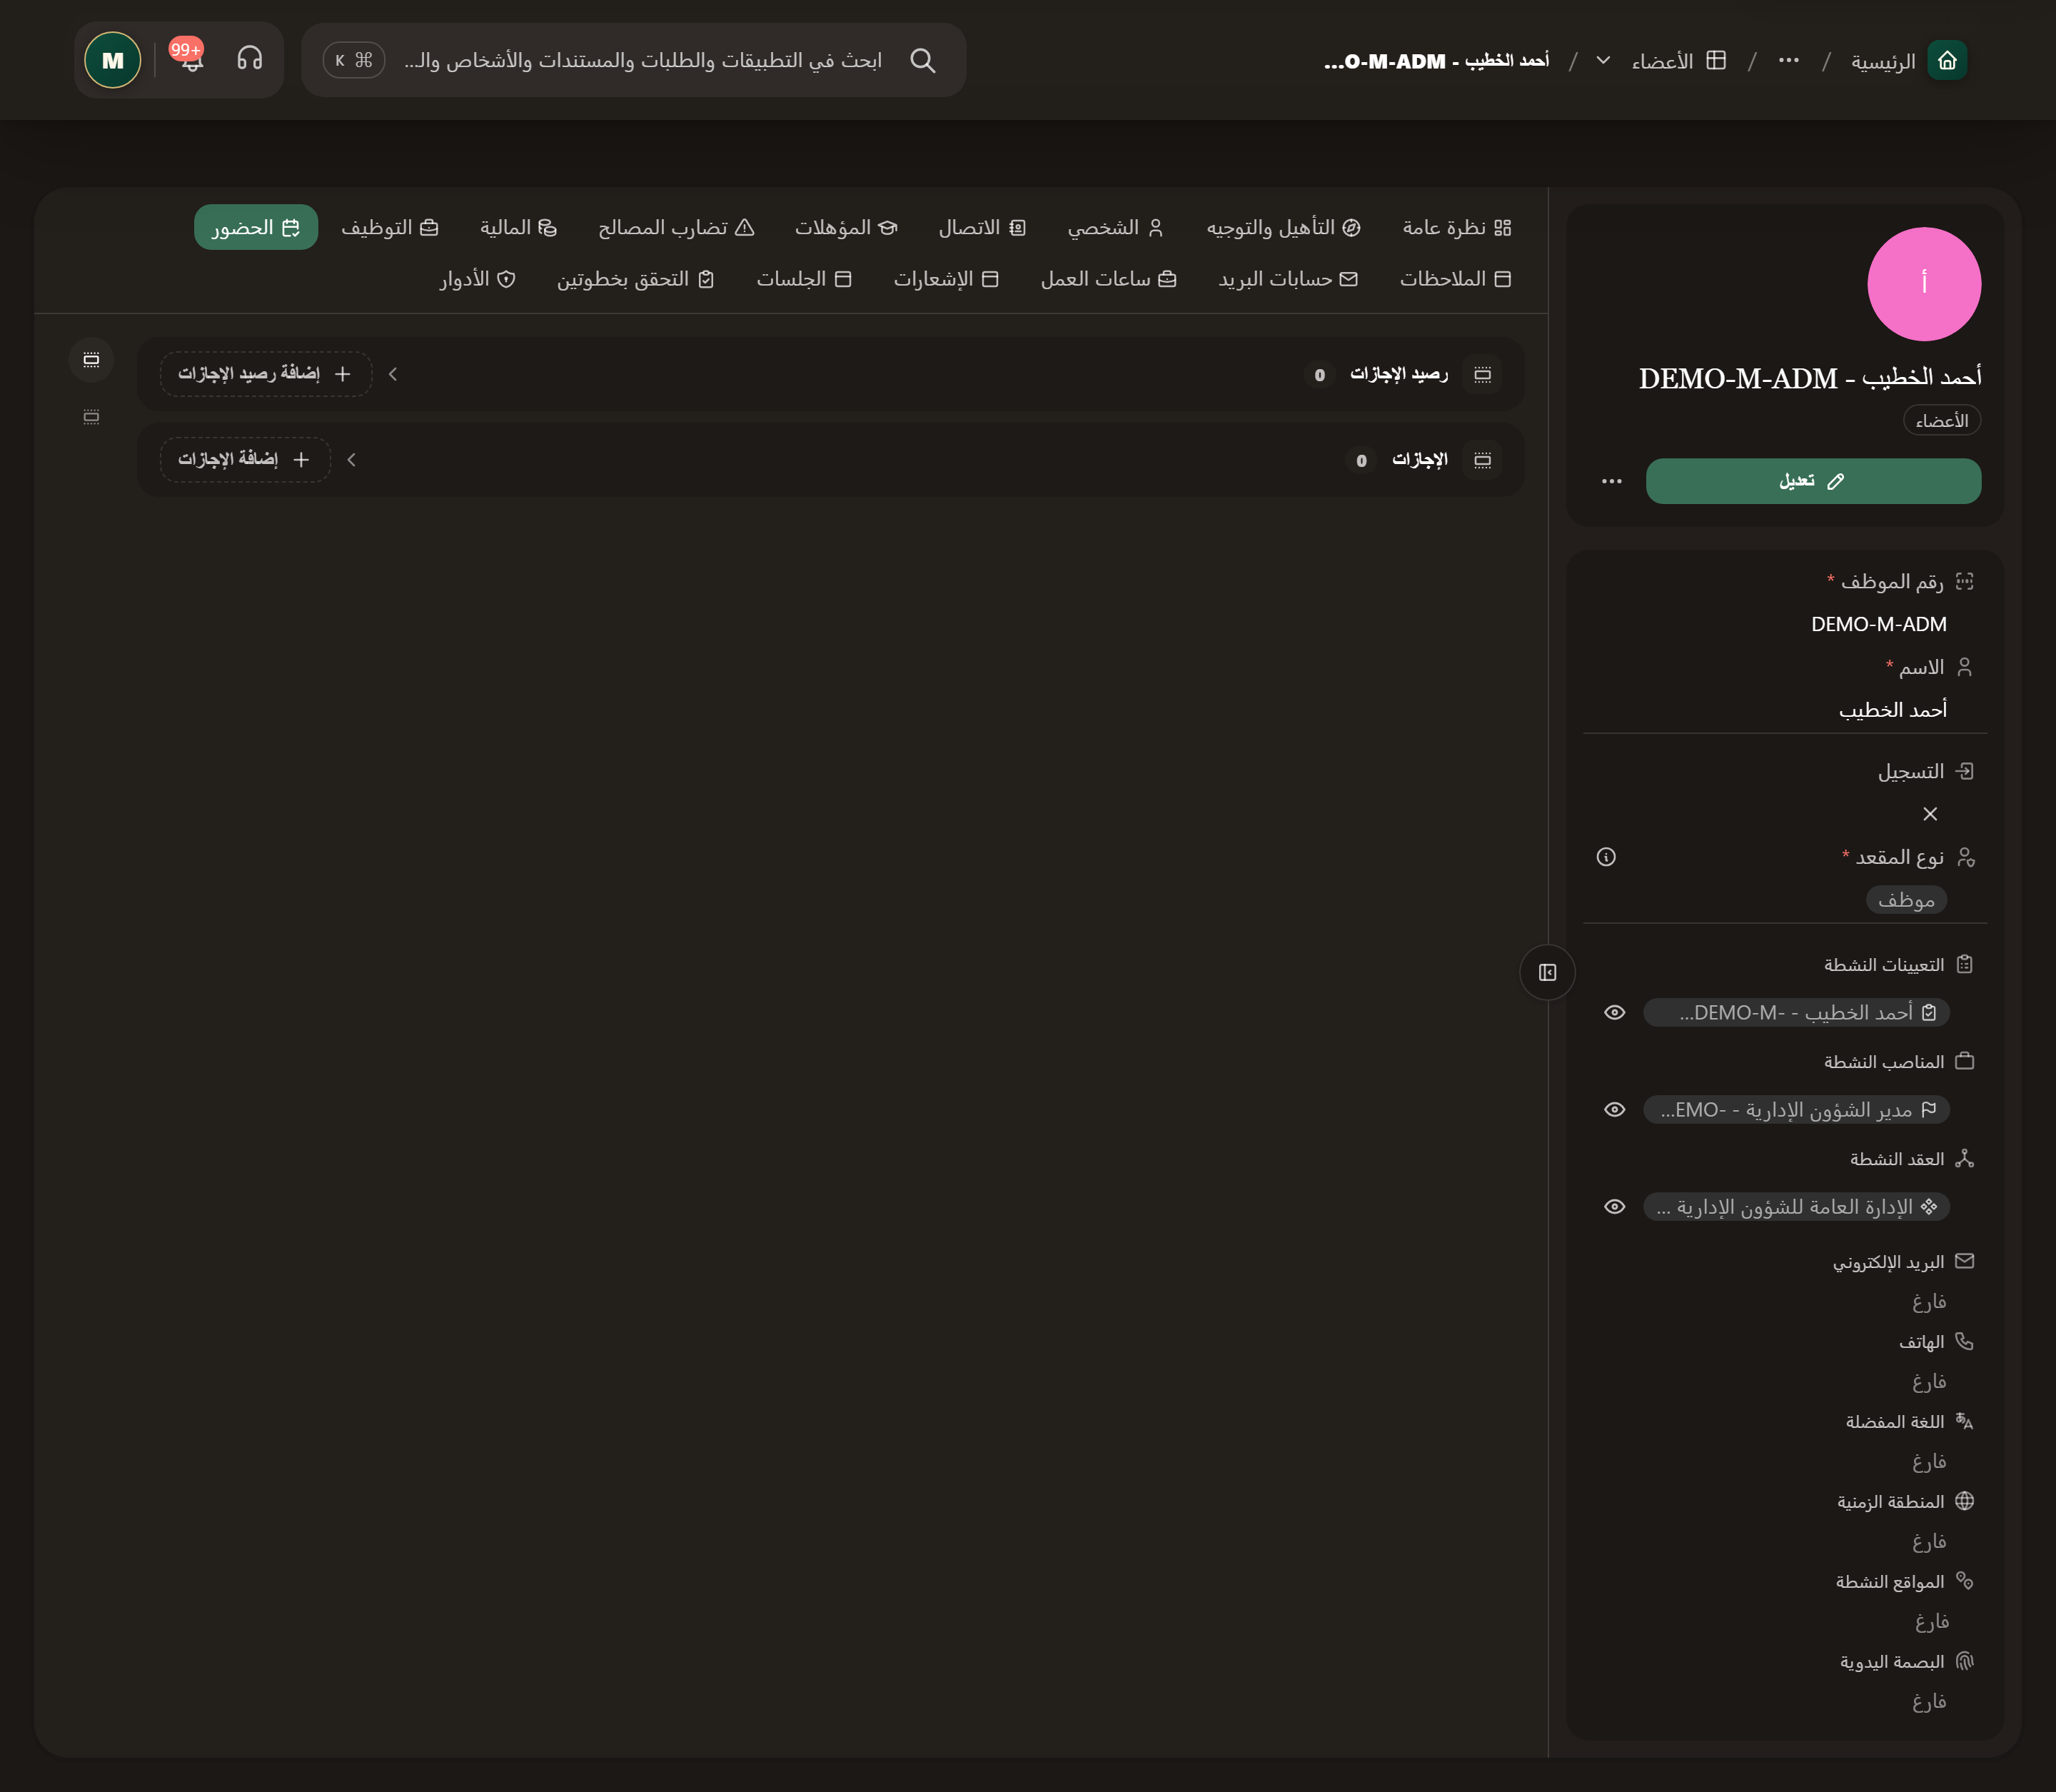
\includegraphics[width=0.95\linewidth]{figures/screens/ch03-member-tab9-ar.png}
\caption{ملف الموظف التجريبي — تبويب «الحضور»}
\label{fig:hr-member-tab9}
\end{figure}



\begin{figure}[H]
\centering
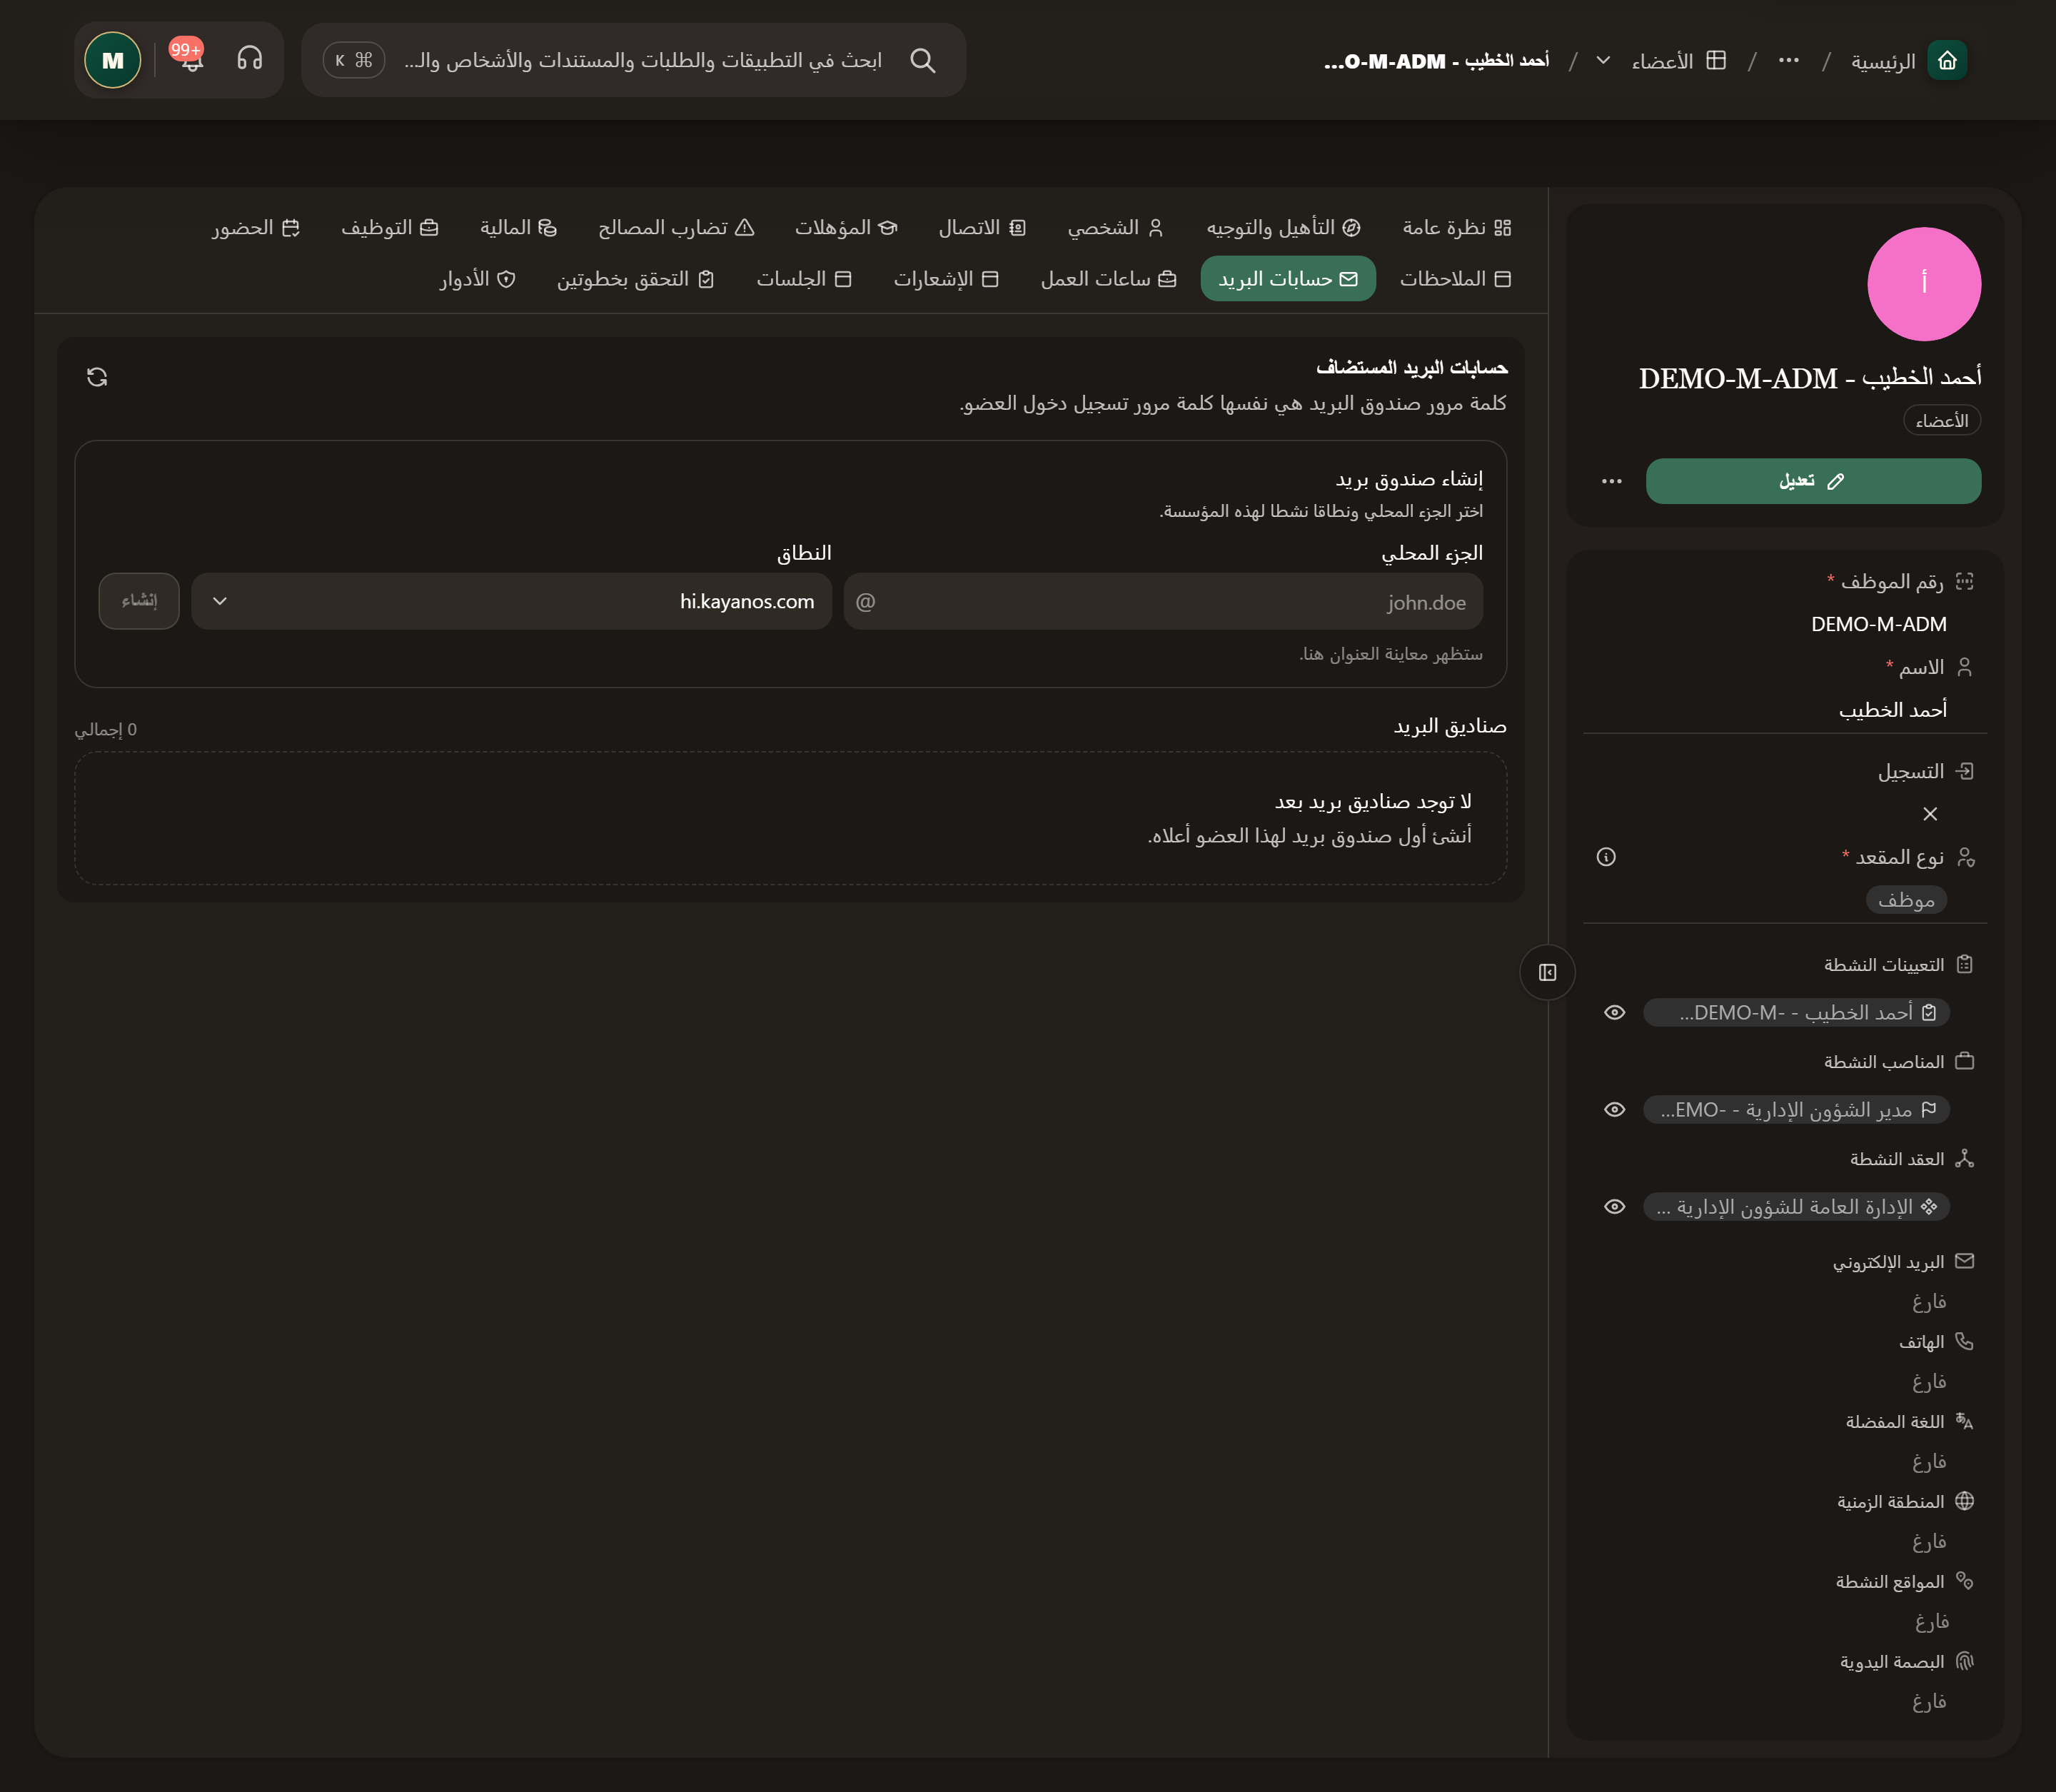
\includegraphics[width=0.95\linewidth]{figures/screens/ch03-member-tab11-ar.png}
\caption{ملف الموظف التجريبي — تبويب «حسابات البريد»}
\label{fig:hr-member-tab11}
\end{figure}

\begin{figure}[H]
\centering
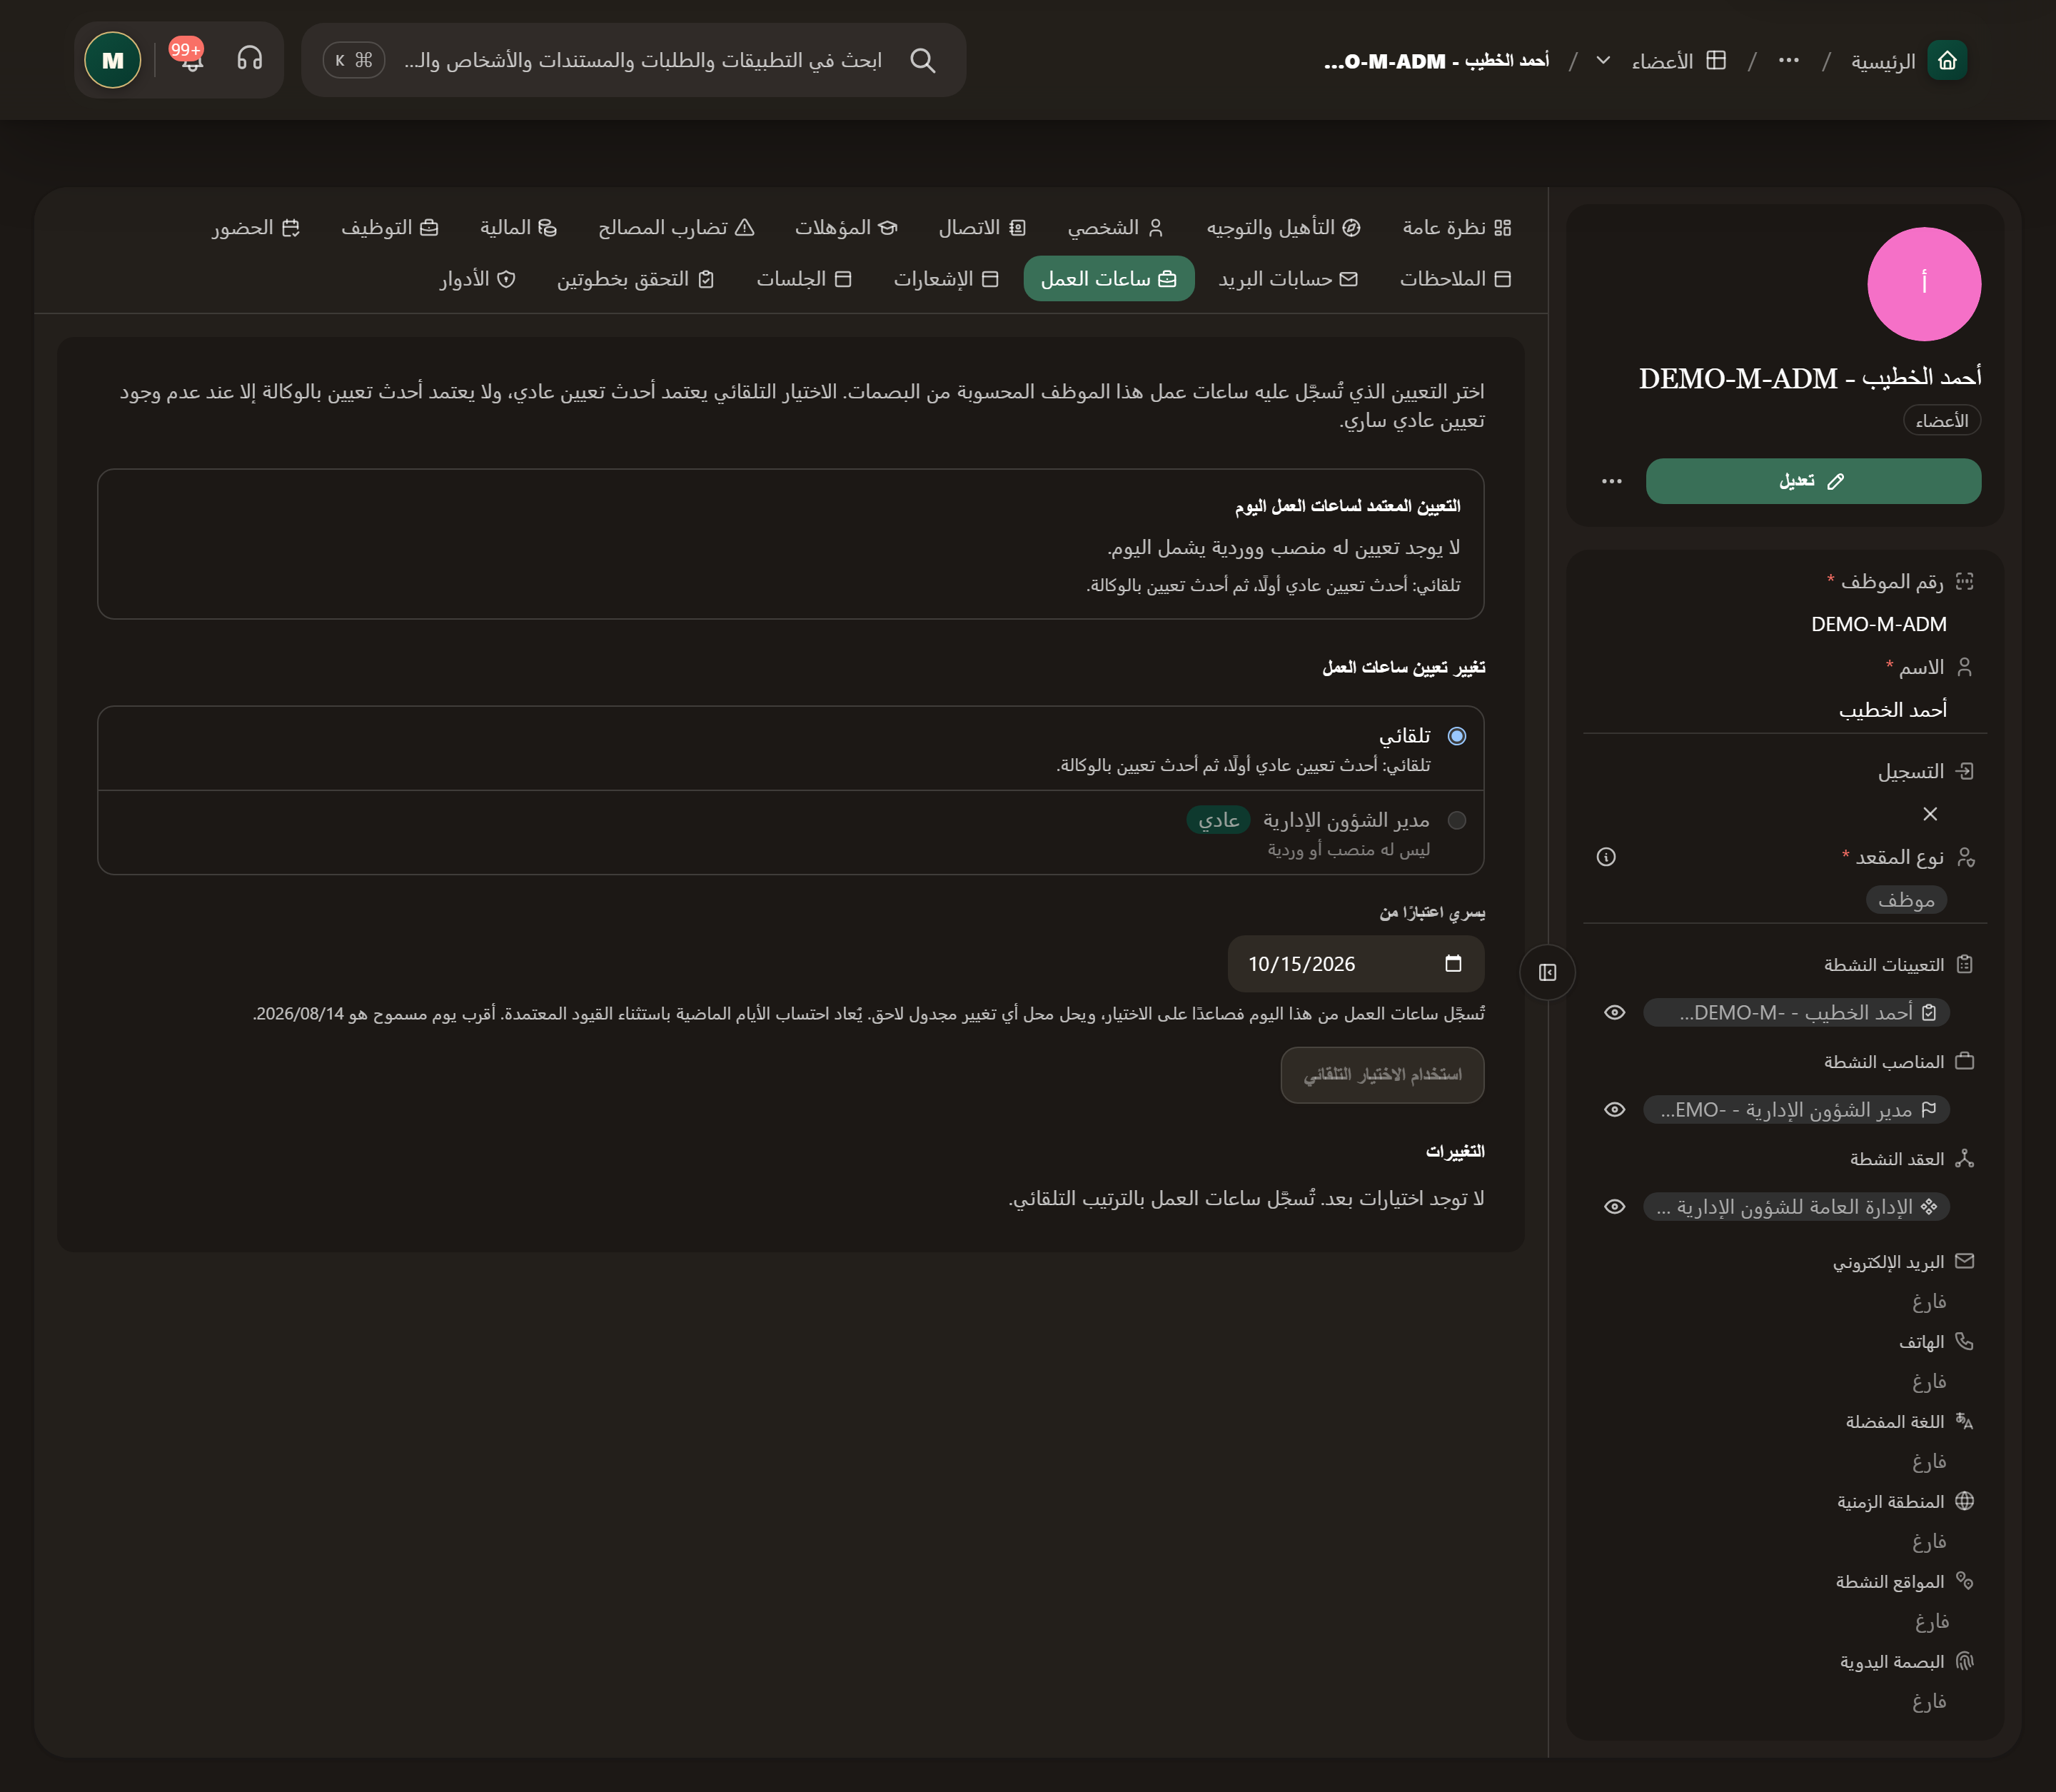
\includegraphics[width=0.95\linewidth]{figures/screens/ch03-member-tab12-ar.png}
\caption{ملف الموظف التجريبي — تبويب «ساعات العمل»}
\label{fig:hr-member-tab12}
\end{figure}

\begin{figure}[H]
\centering
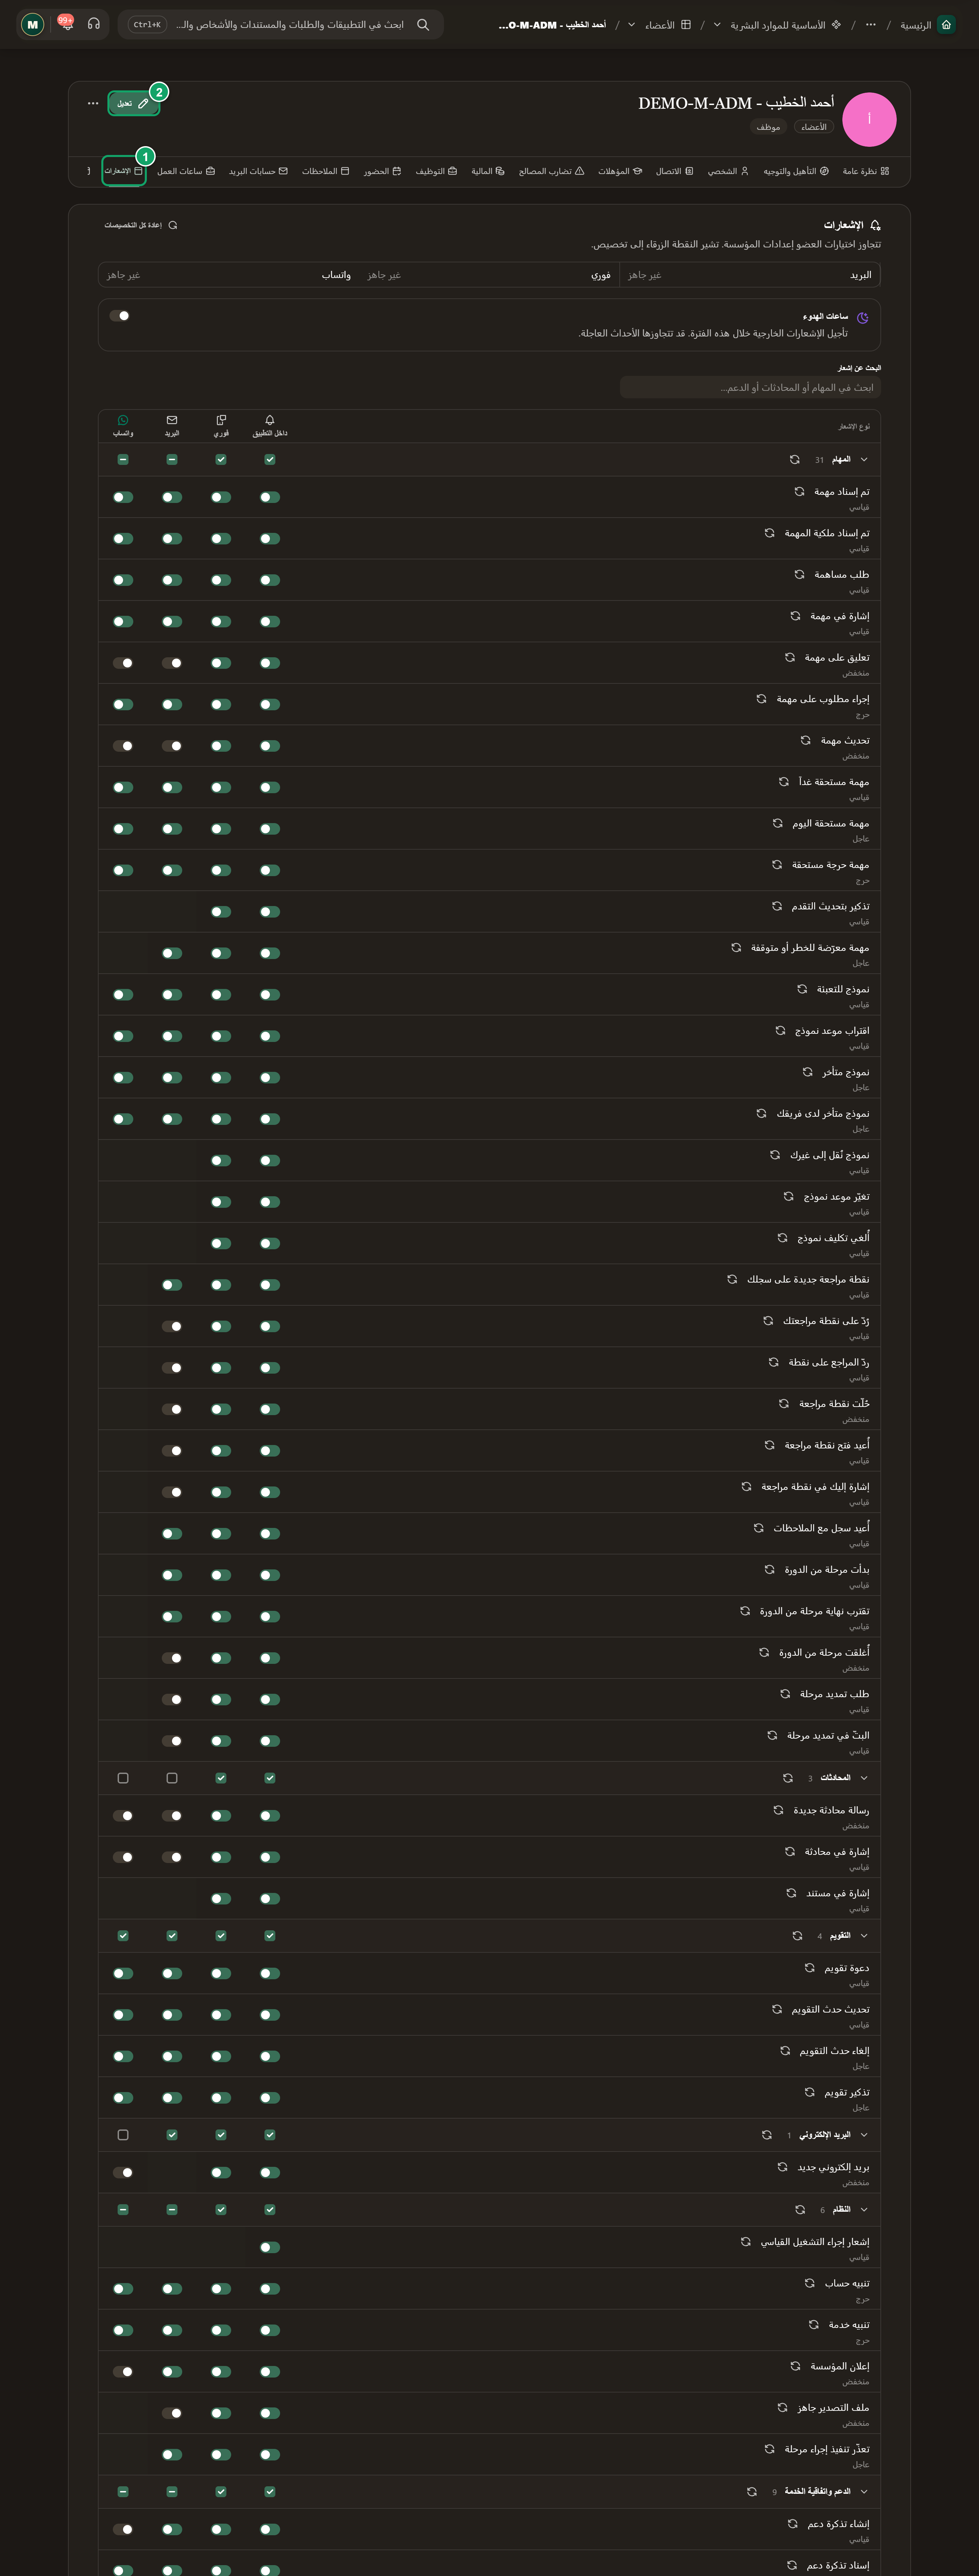
\includegraphics[width=0.95\linewidth]{figures/screens/ch03-member-tab13-ar.png}
\caption{ملف الموظف التجريبي — تبويب «الإشعارات»}
\label{fig:hr-member-tab13}
\end{figure}

\begin{figure}[H]
\centering
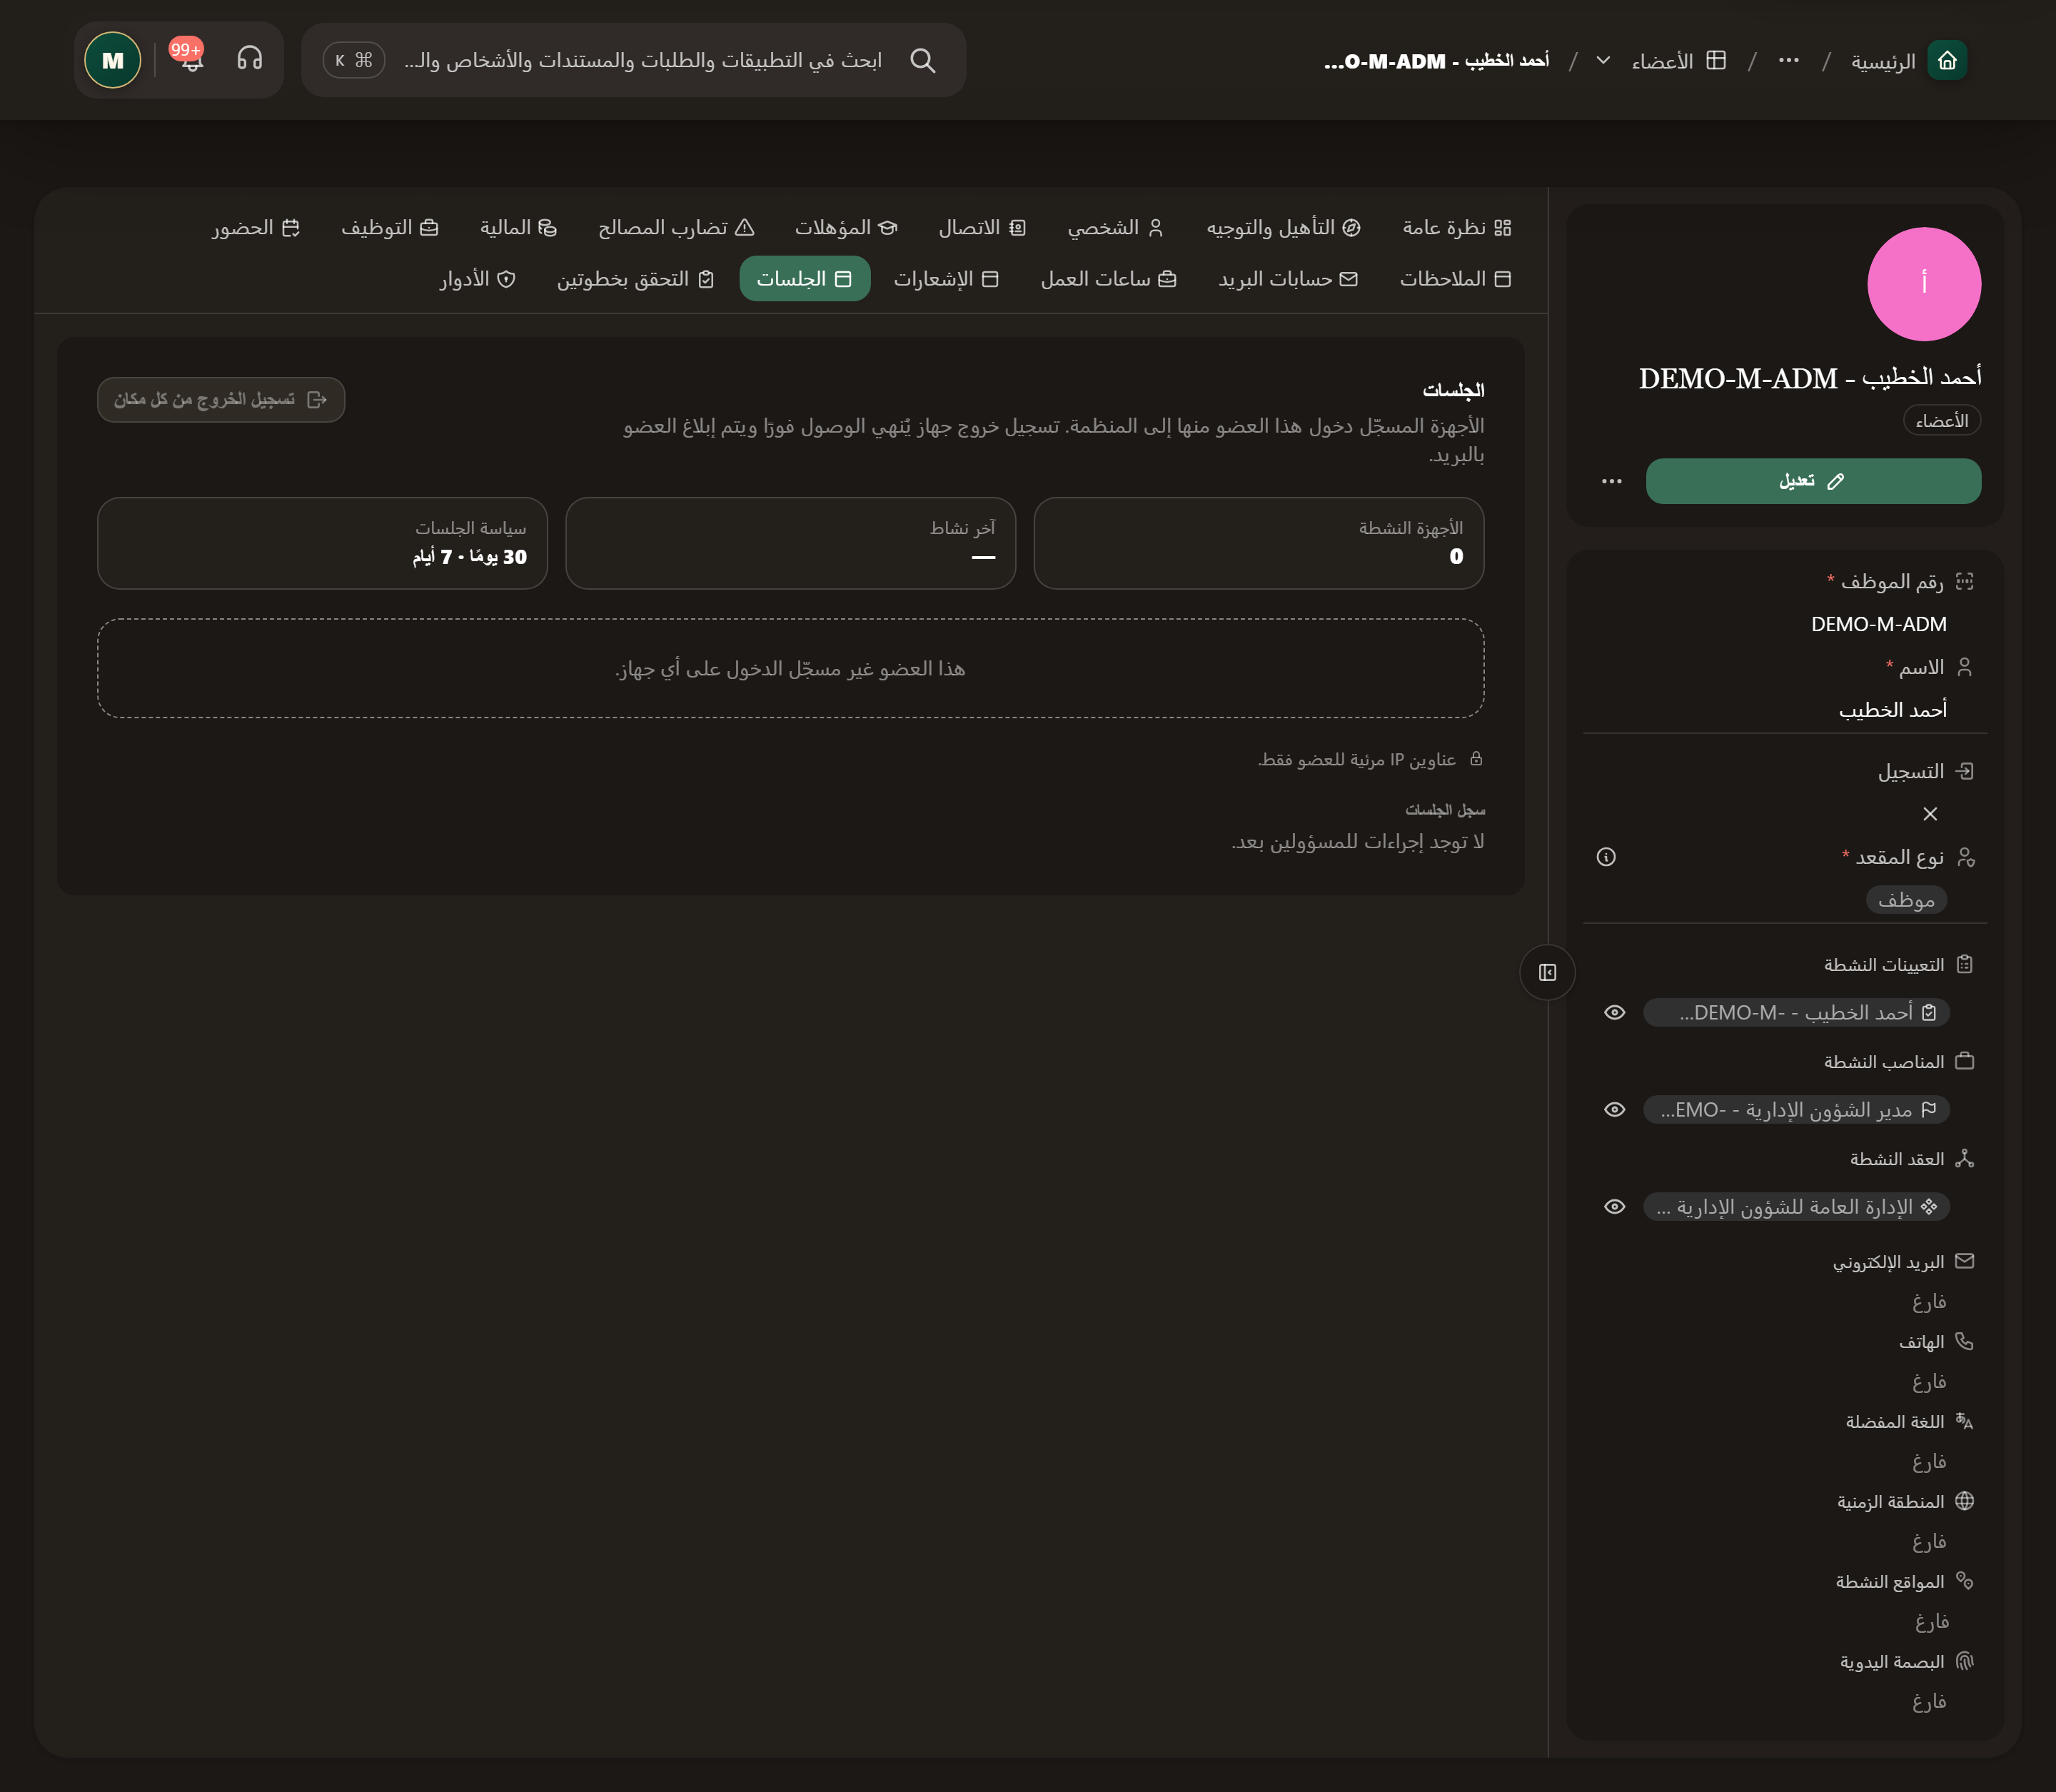
\includegraphics[width=0.95\linewidth]{figures/screens/ch03-member-tab14-ar.png}
\caption{ملف الموظف التجريبي — تبويب «الجلسات»}
\label{fig:hr-member-tab14}
\end{figure}

\begin{figure}[H]
\centering
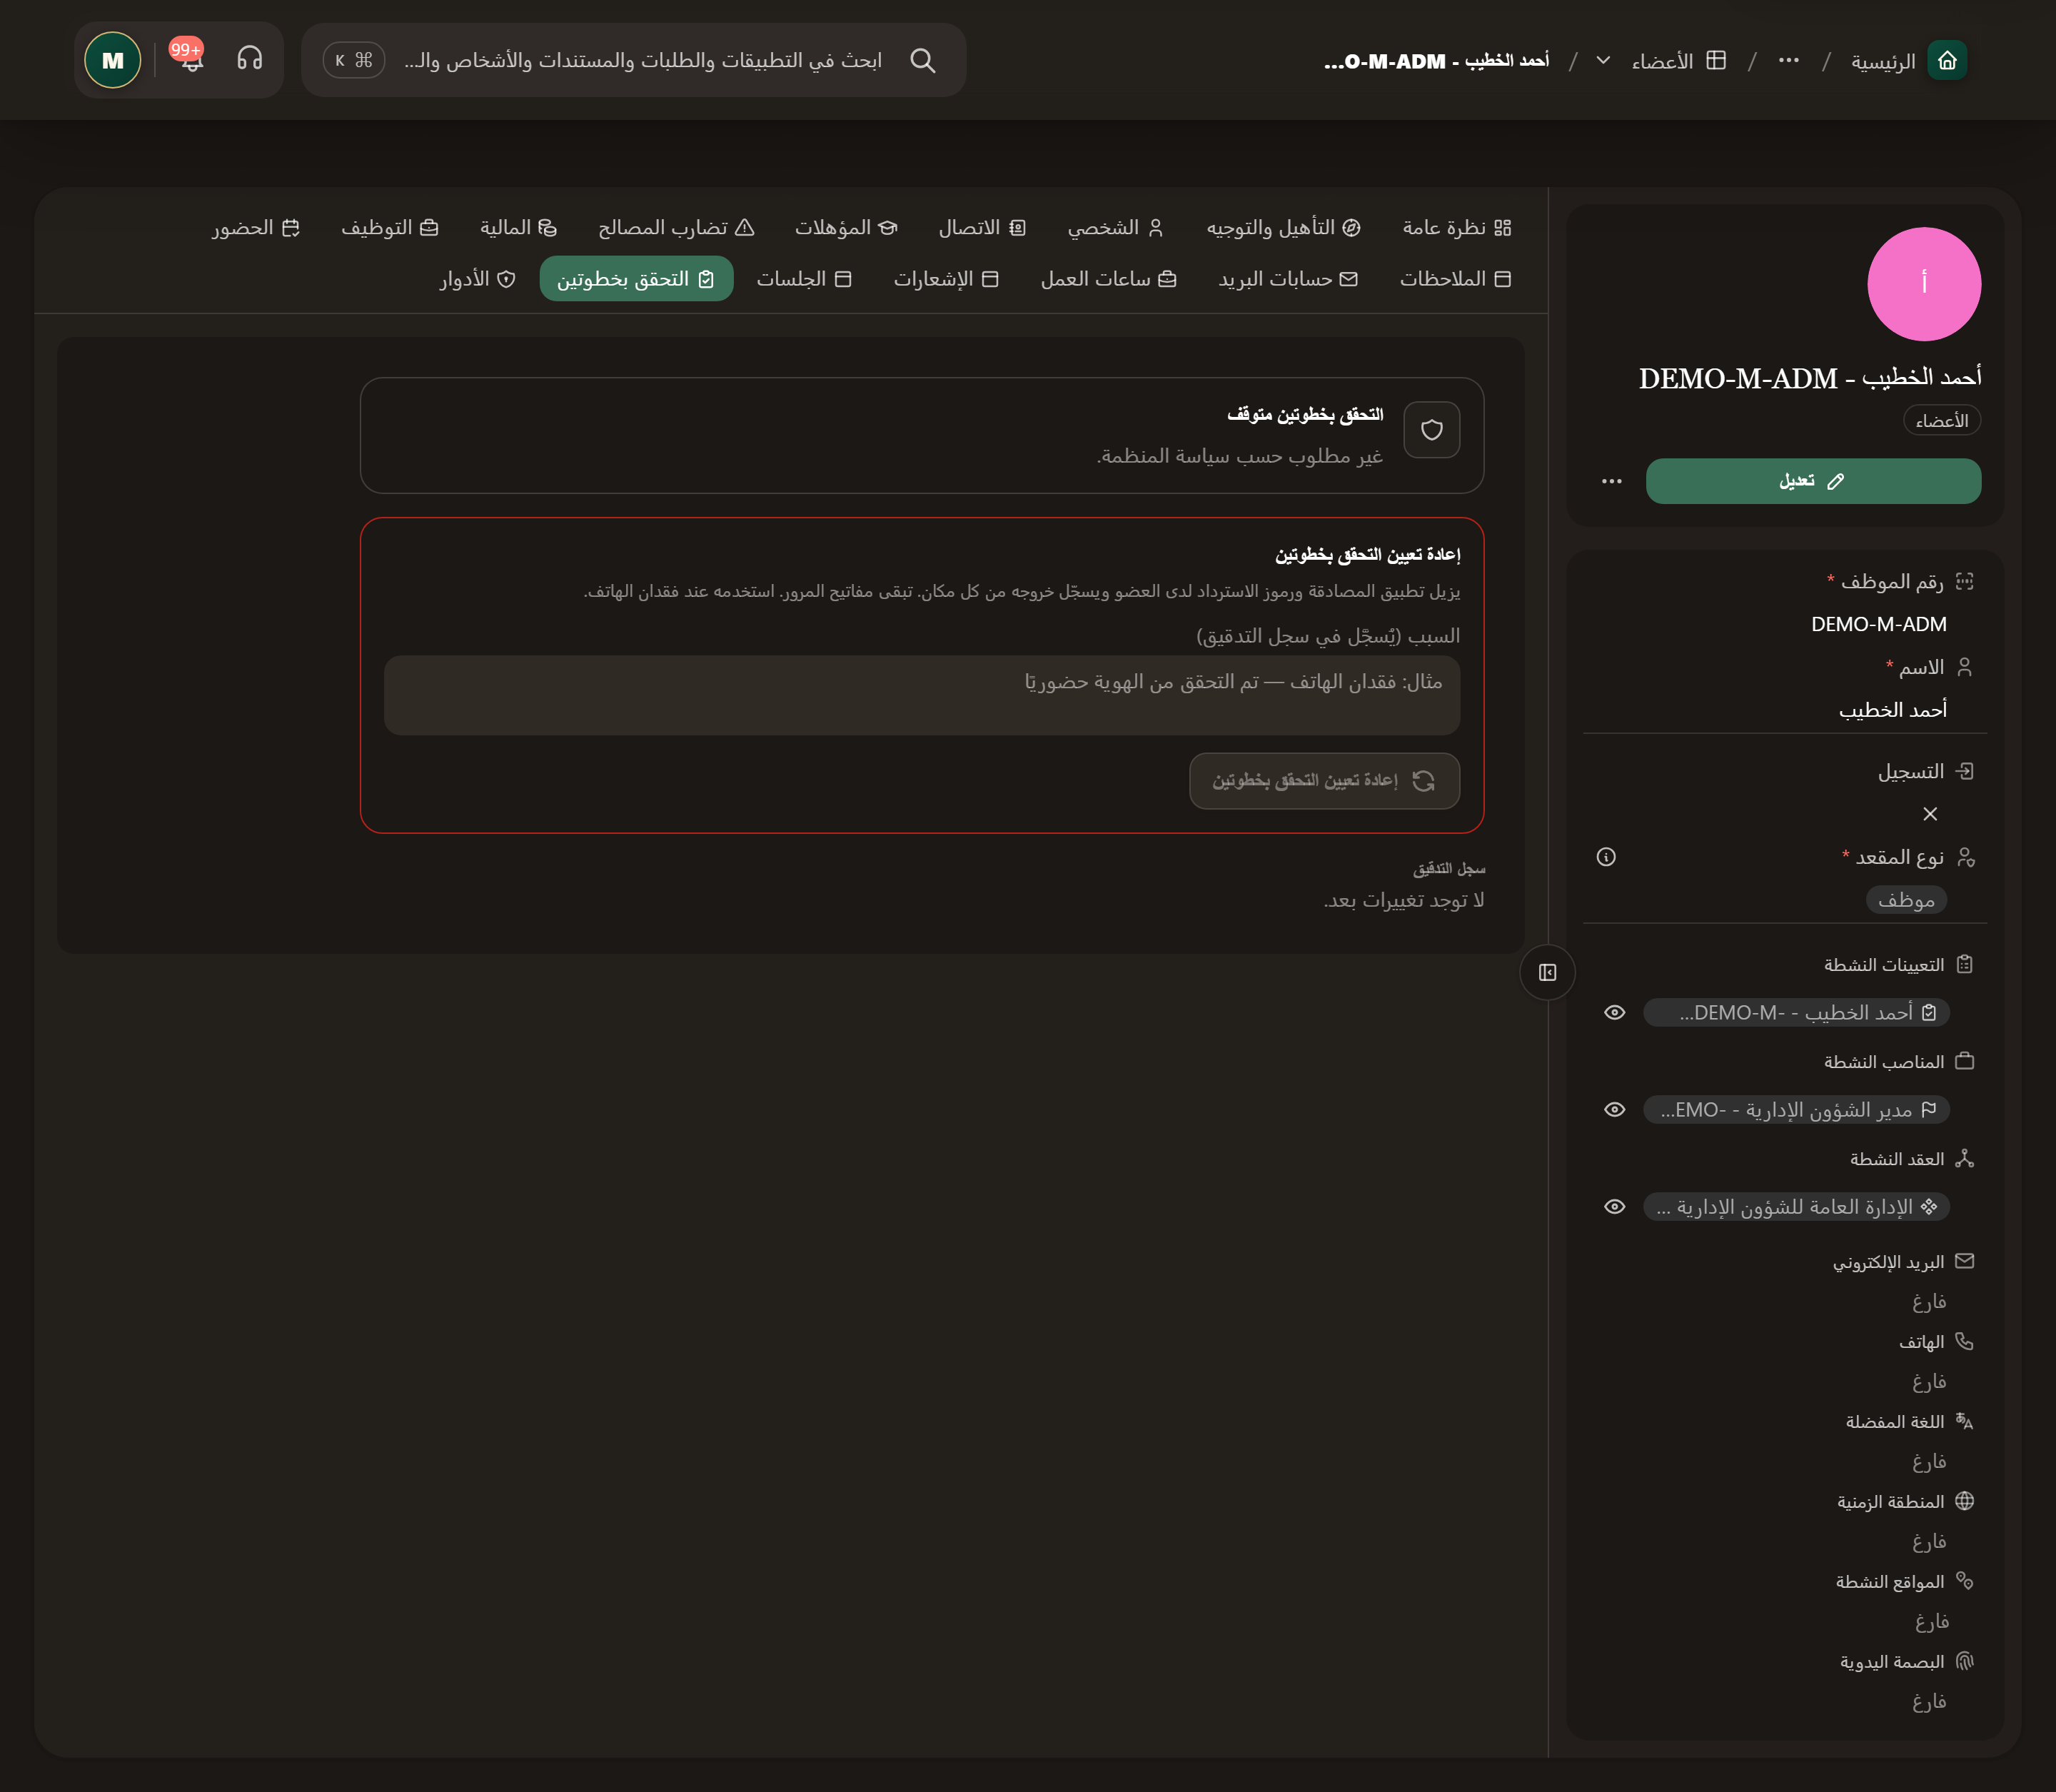
\includegraphics[width=0.95\linewidth]{figures/screens/ch03-member-tab15-ar.png}
\caption{ملف الموظف التجريبي — تبويب «التحقق بخطوتين»}
\label{fig:hr-member-tab15}
\end{figure}

\begin{figure}[H]
\centering
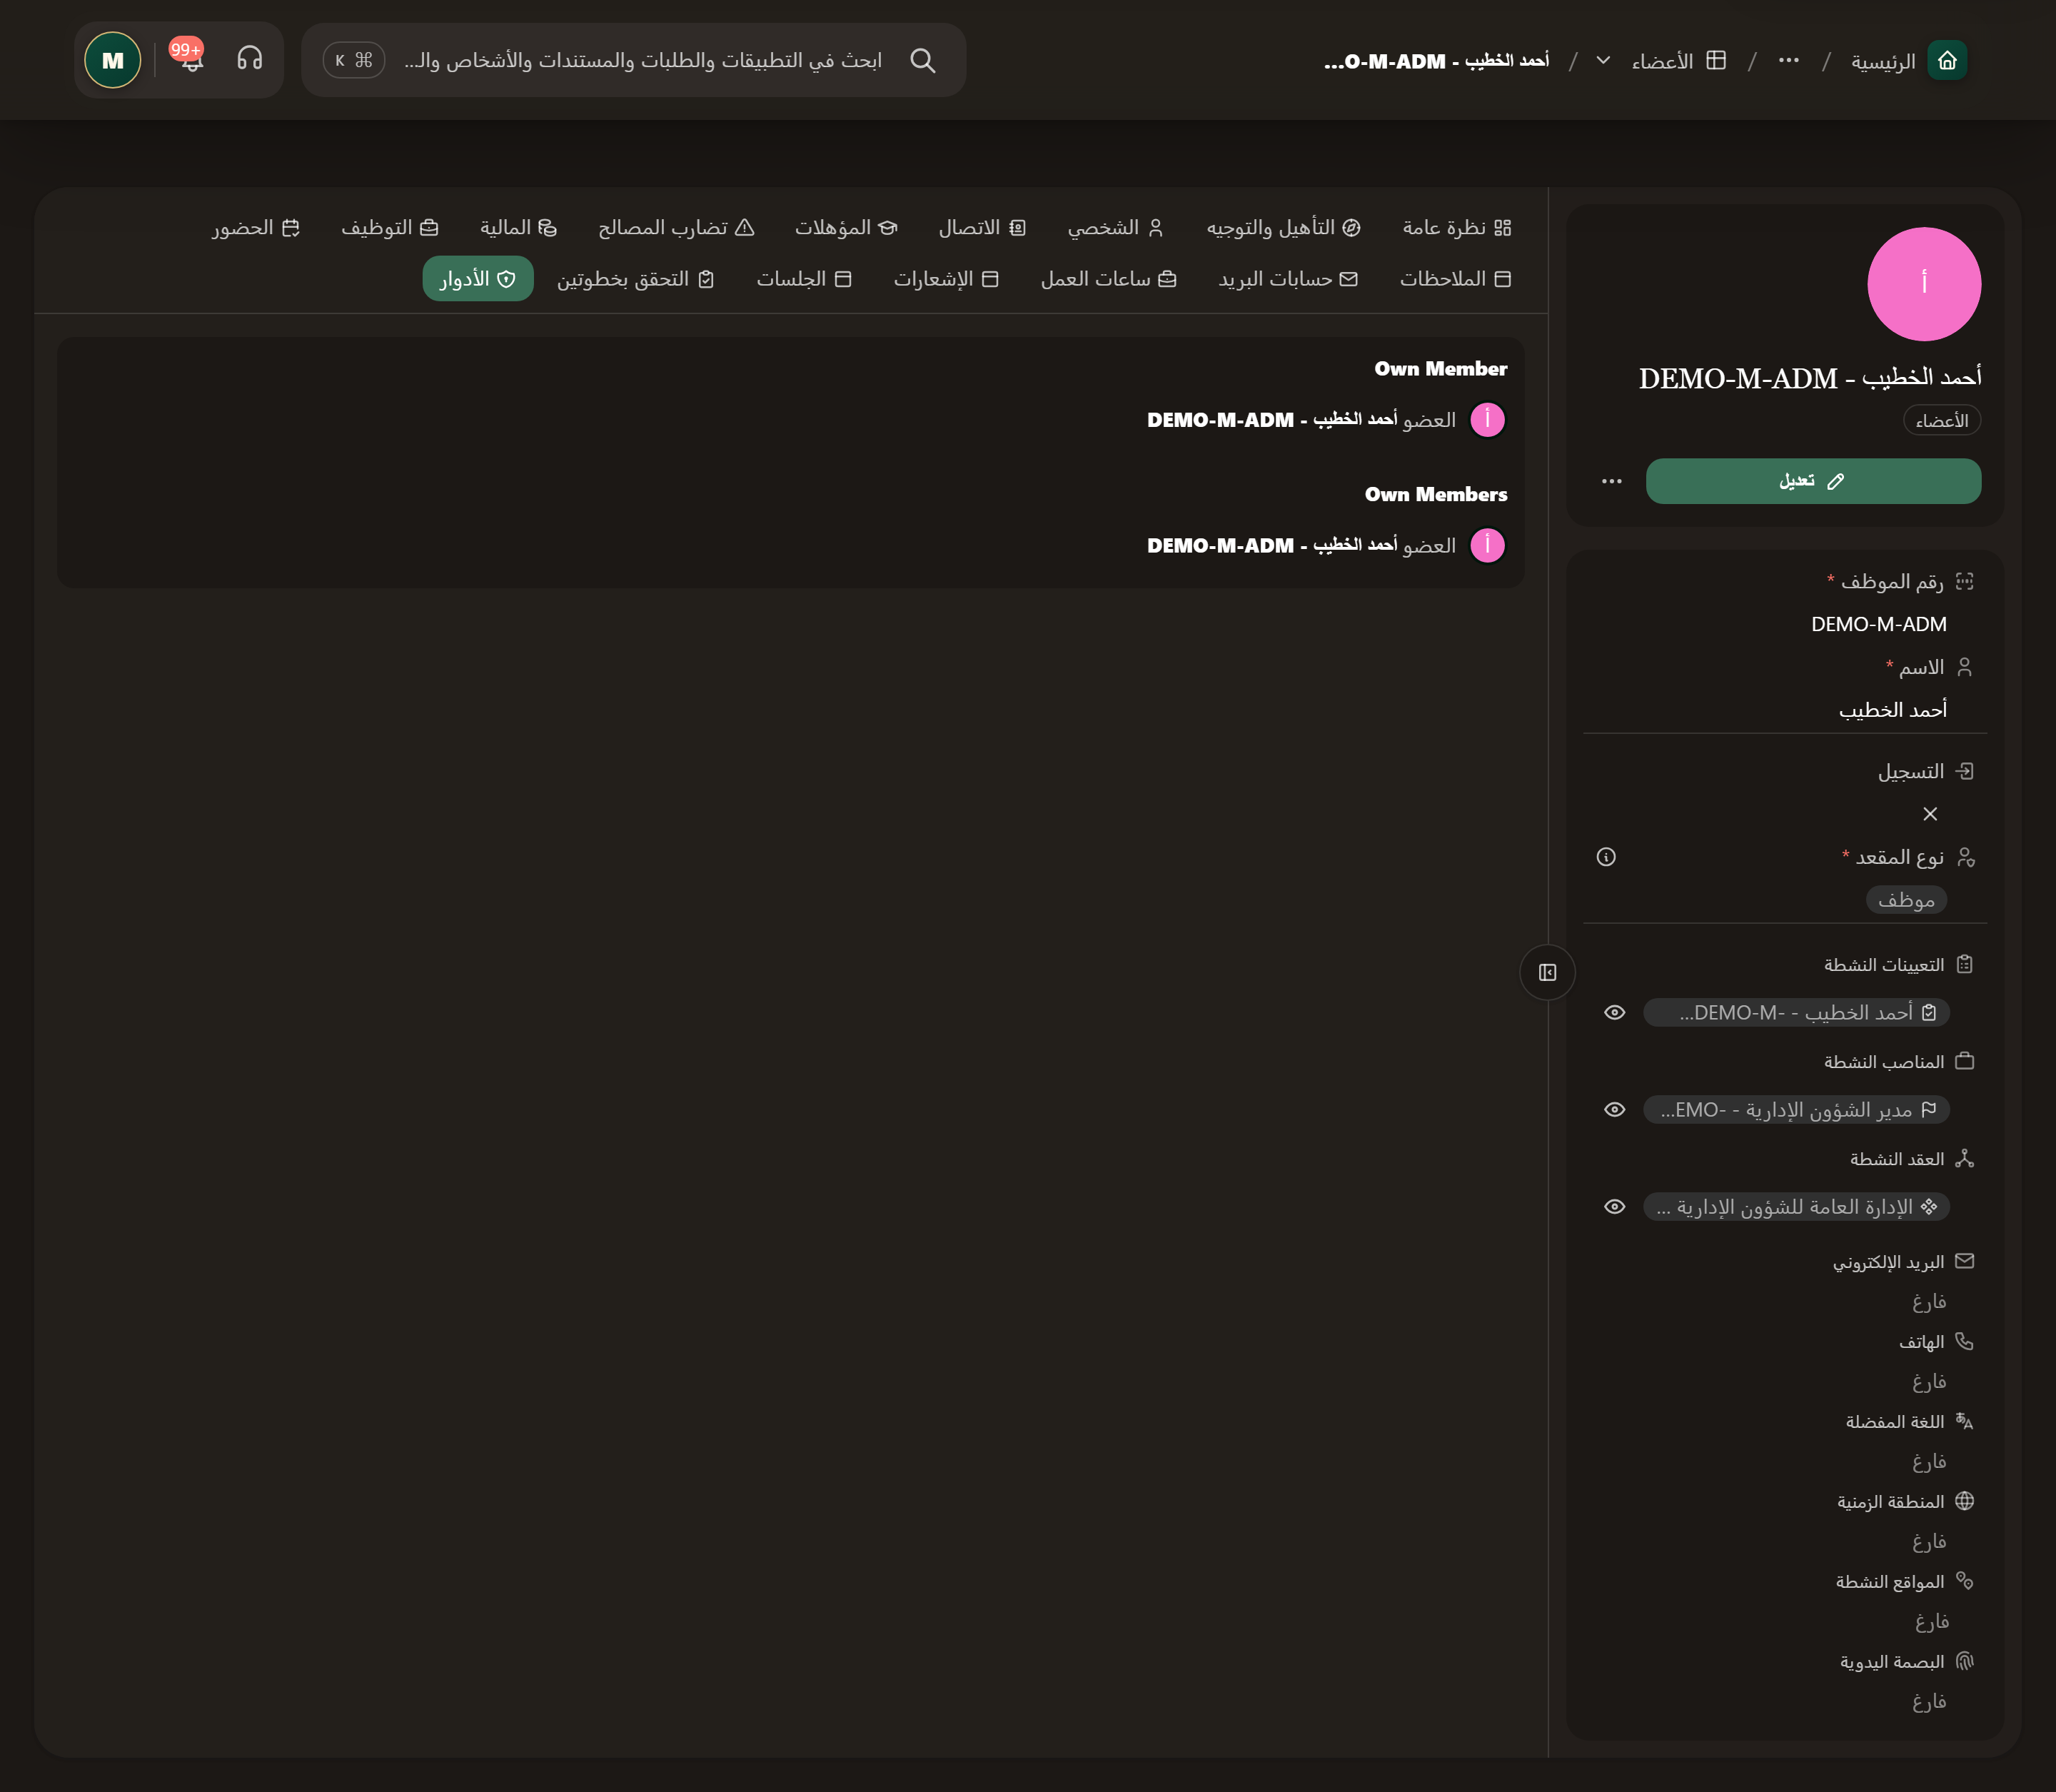
\includegraphics[width=0.95\linewidth]{figures/screens/ch03-member-tab16-ar.png}
\caption{ملف الموظف التجريبي — تبويب «الأدوار»}
\label{fig:hr-member-tab16}
\end{figure}

\clearpage
\section{المناصب}
\label{sec:hr-feature-positions}

المنصب وظيفة مثل مدير الموارد البشرية. تحدد فيه المنصب الذي يتبعه، وقسمه وموقعه ودرجته؛ ويحدد التعيين من يشغله.

\textbf{متى تفيد؟} عرّف الوظيفة مرة واحدة، ثم تابع من يشغلها، أو إن كانت شاغرة. \textbf{المسار:} «الموارد البشرية» / «القوى العاملة» / «المناصب».

\begin{figure}[H]
\centering
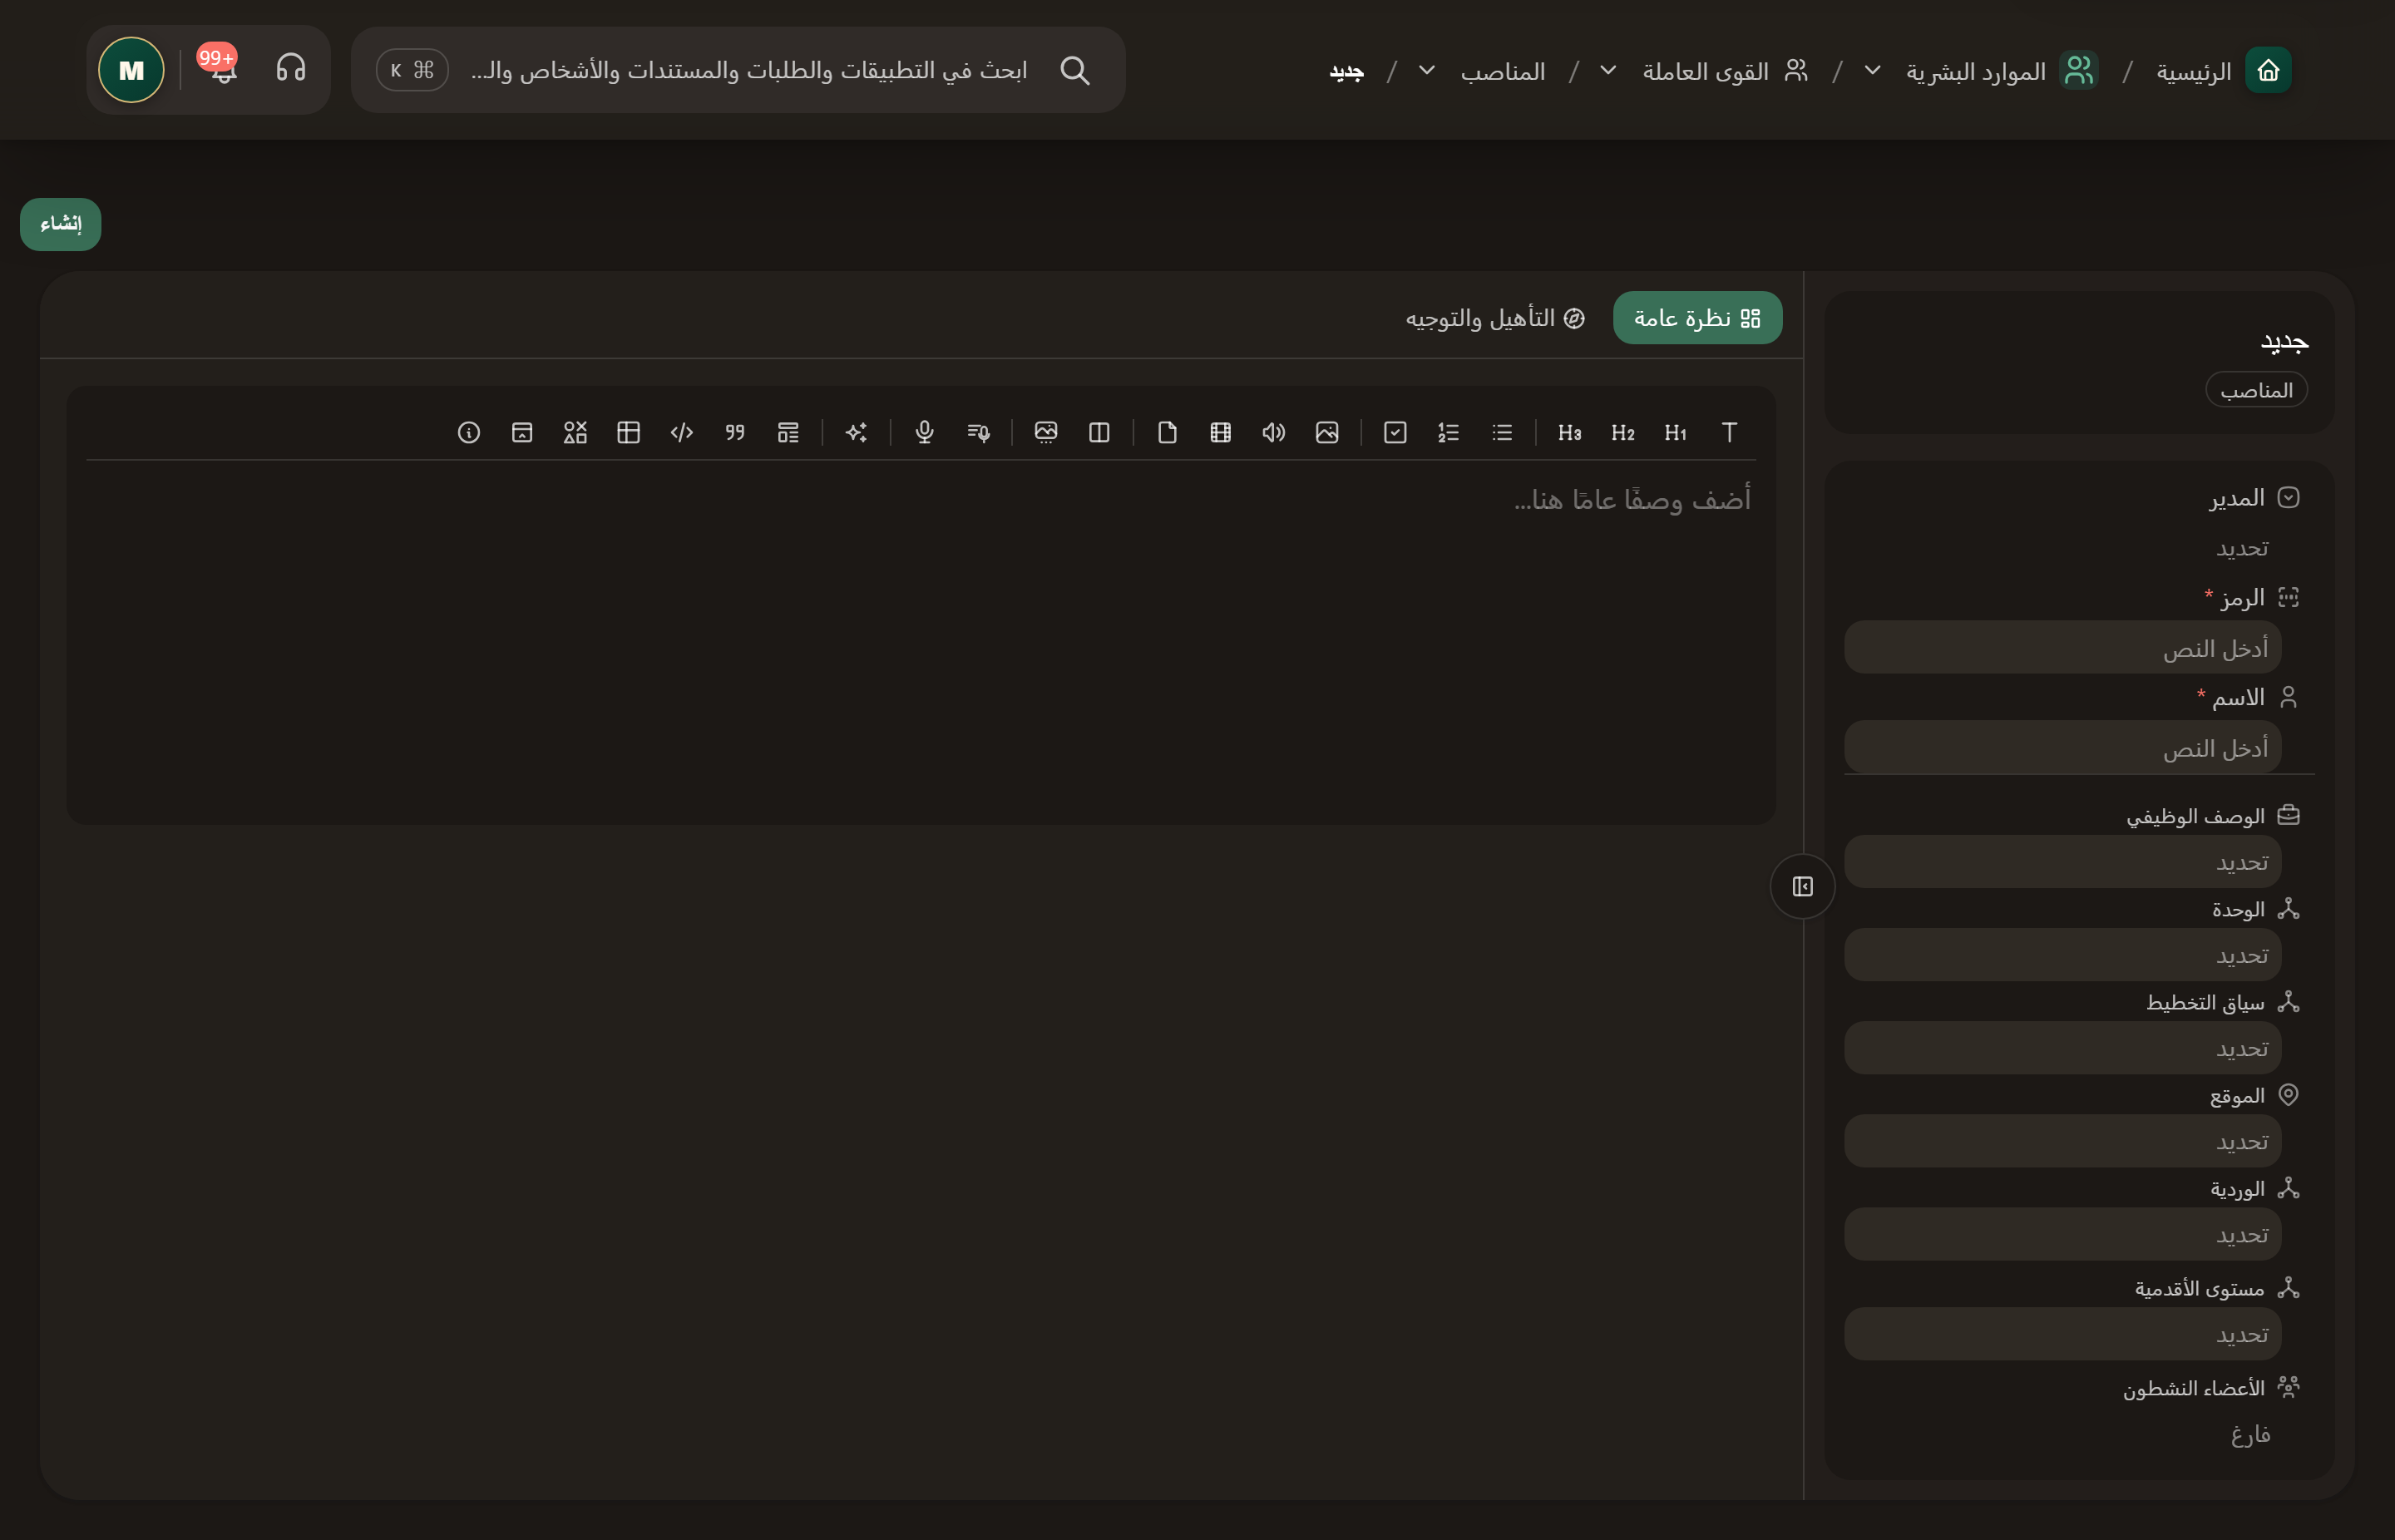
\includegraphics[width=0.95\linewidth]{figures/screens/ch02-position-fields-ar.png}
\caption{المناصب: نموذج من بيئة الاختبار؛ لم يُحفظ}
\label{fig:hr-feature-positions-screen}
\end{figure}

\begin{table}[H]
\centering
\caption{ما الذي تسجله في المنصب؟}
\label{tab:hr-feature-positions-data}
\rcZebra
\begin{tabularx}{\linewidth}{R{3.6cm} Y}
\rcHeaderRow
\thh{الحقل} & \thh{ما الذي تضيفه؟}\\
الرمز والاسم & \req{}؛ مثل \en{HZN-P-01} مدير الموارد البشرية.\\
المدير & المنصب الذي يتبعه هذا المنصب؛ ومنه تُبنى شجرة الهيكل الوظيفي.\\
الوصف الوظيفي & المهام والمسؤوليات؛ تختاره من قائمة الأوصاف أو تكتب وصفاً جديداً.\\
الوحدة والموقع & القسم ومكان العمل \opt{}.\\
الوردية والمستوى الوظيفي & دوام الوظيفة ودرجتها في سلم الراتب \opt{}.\\
سياق التخطيط & خطة أو مشروع أو برنامج ترتبط به الوظيفة \opt{}.\\
\end{tabularx}
\end{table}

\subsection{ما الذي يمكنك فعله؟}

\begin{itemize}
  \item عرض «شجرة»: ابحث بالمنصب أو الرمز أو الشخص، وسّع الفروع أو اطوِها، واختر «إظهار هذا الفرع فقط».
  \item كل بطاقة في الشجرة تبيّن شاغل المنصب أو «شاغر»، وعدد المناصب التابعة.
  \item يعرض النظام شاغلي المنصب الحاليين \gen{}.
\end{itemize}

\begin{figure}[H]
\centering
\begin{tikzpicture}[node distance=0.5cm,stepBox/.append style={minimum width=6.5cm,text width=6.1cm,minimum height=0.8cm}]
  \node[stepBox] (a) {\RL{تعريف الوظيفة}};
  \node[stepBox,below=of a] (b) {\RL{اختيار القسم والموقع}};
  \node[stepBox,below=of b] (c) {\RL{تعيين الموظف}};
  \draw[flowsTo] (a) -- (b);
  \draw[flowsTo] (b) -- (c);
\end{tikzpicture}
\rclegend
\caption{خطوات الاستخدام؛ الأسهم لا تعني معالجة تلقائية}
\label{fig:hr-feature-positions-flow}
\end{figure}

\subsection{جرّب وراجع}

\begin{enumerate}
  \item جهّز القسم والموقع إن أردت ربطهما. افتح «المناصب» وتأكد أن الوظيفة غير موجودة.
  \item أضف «مدير الموارد البشرية» برمز \en{HZN-P-01}، واختر قسم الموارد البشرية والمقر الرئيسي بدمشق، ثم احفظ.
\end{enumerate}

\textbf{تحقق:} أعد فتح المنصب وتحقق من روابطه، ثم افتح الشجرة. إنشاء المنصب لا يعيّن سارة فيه.

\begin{figure}[H]
\centering
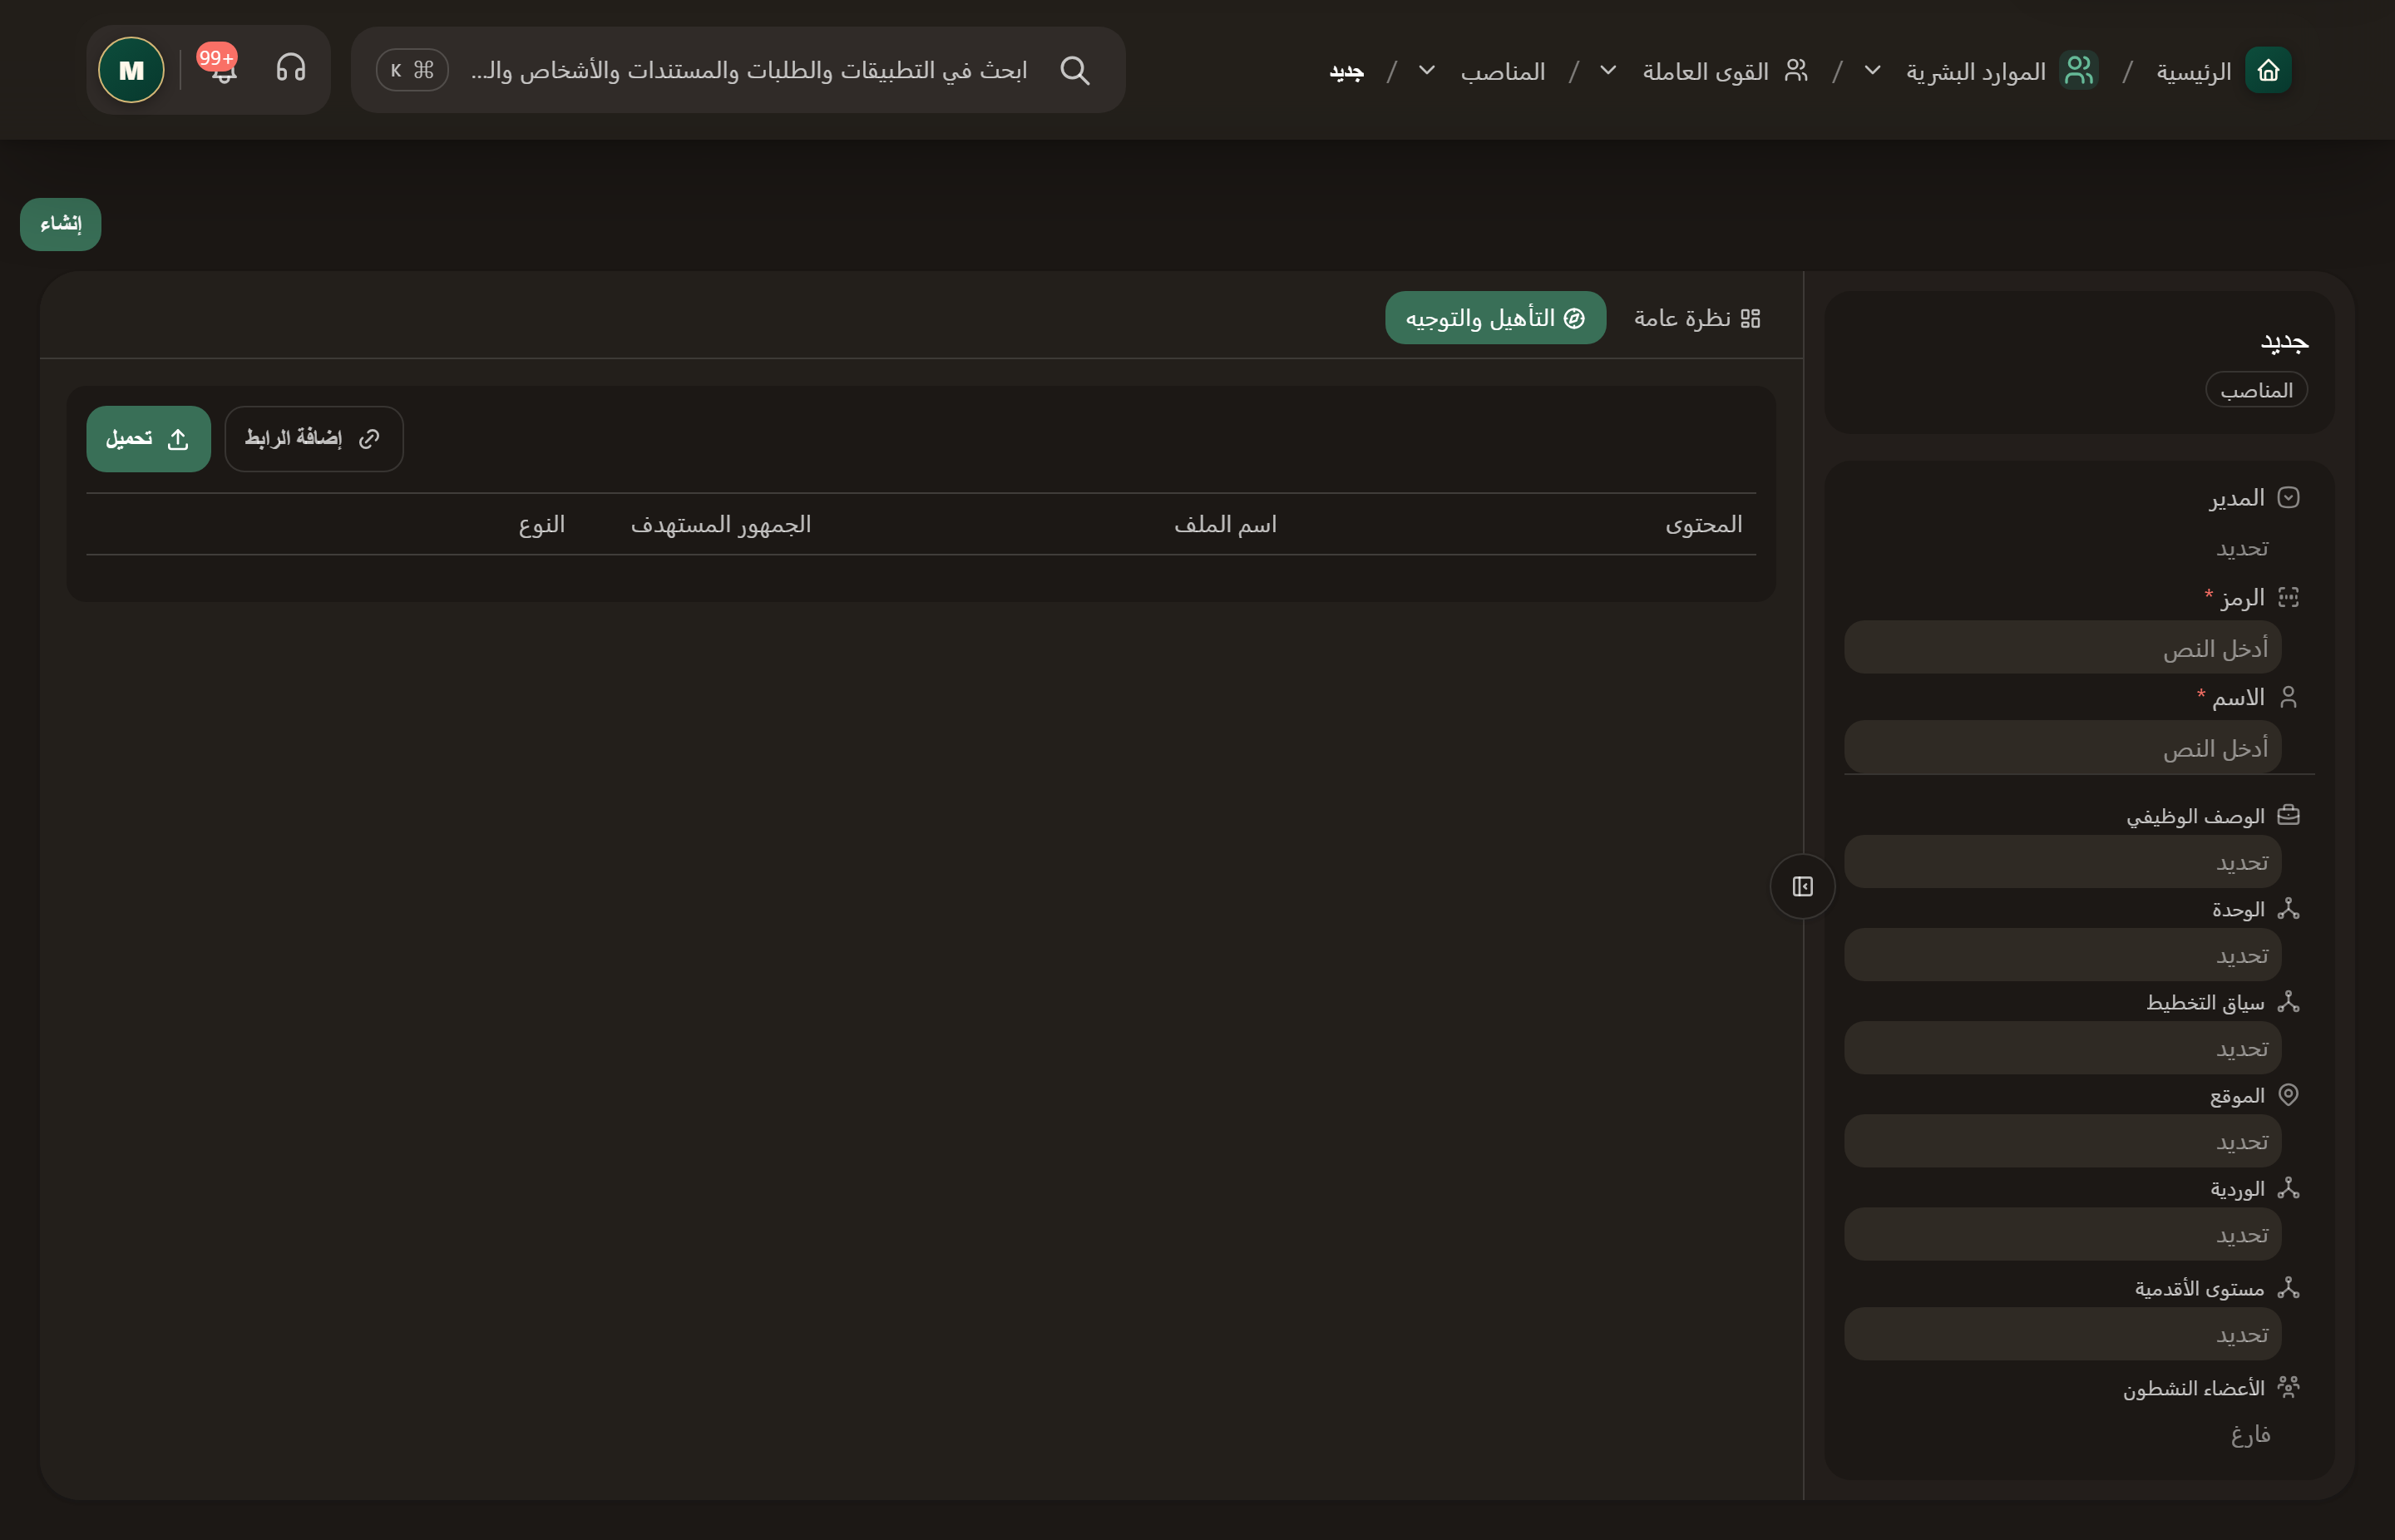
\includegraphics[width=0.95\linewidth]{figures/screens/ch02-position-fields-tab2-ar.png}
\caption{تبويب «التأهيل والتوجيه» كاملاً؛ نموذج غير محفوظ}
\label{fig:hr-positions-fulltab1}
\end{figure}

\clearpage
\section{التعيينات}
\label{sec:hr-feature-assignments}

التعيين يسجل من يشغل المنصب، ومنذ متى، وبأي عقد وراتب ووردية.

\textbf{متى تفيد؟} عند انضمام سارة أو انتقالها إلى وظيفة أخرى. يحفظ التعيين وظائفها وتواريخها منفصلة عن ملفها الشخصي. \textbf{المسار:} «الموارد البشرية» / «القوى العاملة» / «التعيينات».

\begin{figure}[H]
\centering
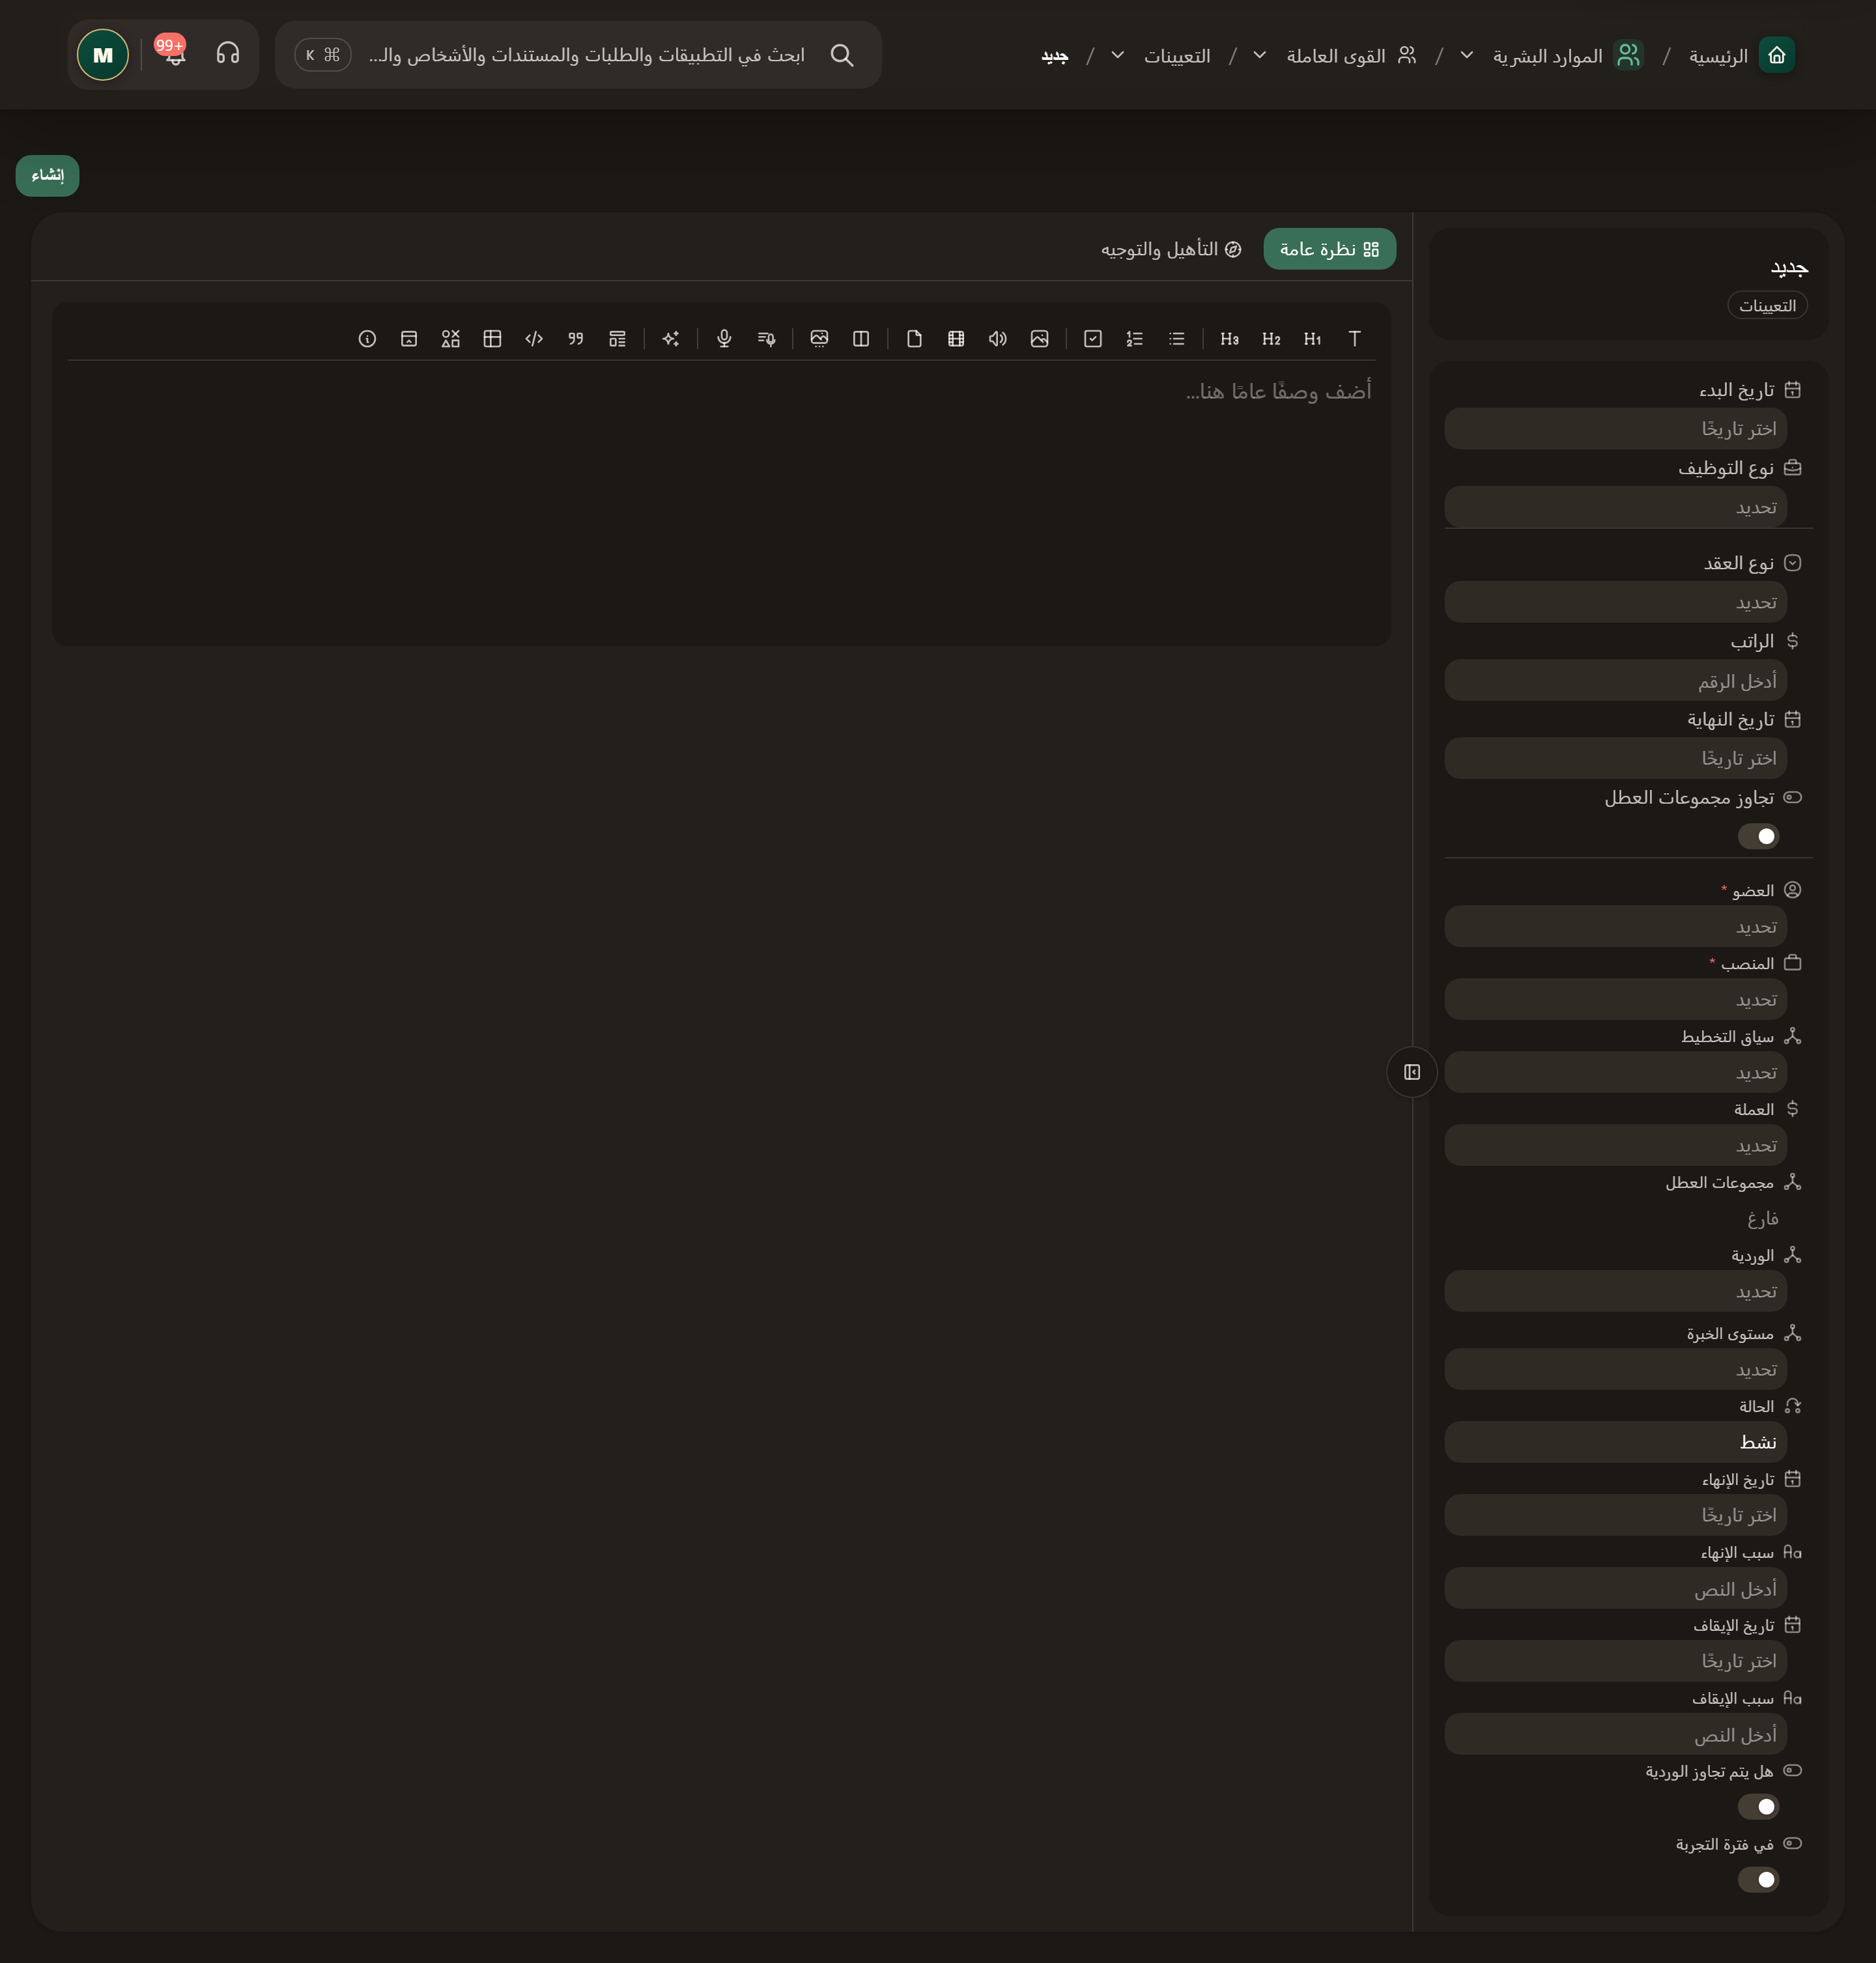
\includegraphics[width=0.95\linewidth]{figures/screens/ch02-assignment-fields-ar.png}
\caption{التعيينات: نموذج من بيئة الاختبار؛ لم يُحفظ}
\label{fig:hr-feature-assignments-screen}
\end{figure}

\begin{table}[H]
\centering
\caption{ما الذي تسجله في التعيين؟}
\label{tab:hr-feature-assignments-data}
\rcZebra
\begin{tabularx}{\linewidth}{R{3.6cm} Y}
\rcHeaderRow
\thh{الجزء} & \thh{ما الذي تضيفه؟}\\
الشخص والوظيفة & العضو \req{} والمنصب \req{}.\\
العقد & نوع التوظيف: موظف، مقاول، متطوع، متدرب، قائم بأعمال، عند الطلب. نوع العقد: دائم، محدد المدة، مؤقت.\\
الفترة & تاريخ البدء وتاريخ النهاية، وفترة التجربة وتاريخ انتهائها.\\
الراتب & الراتب والعملة ومستوى الخبرة.\\
الوقت & الوردية وتجاوزها، ومجموعات العطل وتجاوزها.\\
الحالة & نشط، متوقف، منتهي، مكتمل؛ مع تاريخ الإيقاف أو الإنهاء وسببه.\\
\end{tabularx}
\end{table}

\subsection{ما الذي يمكنك فعله؟}

\begin{itemize}
  \item عرض القائمة جدولاً، أو لوحة كانبان حسب الحالة، أو تقويماً أو خطاً زمنياً حسب تواريخ البدء والنهاية.
  \item ابدأ التعيين من ملف العضو باختيار «إضافة تعيين».
  \item حفظ التعيين يحدّث مناصب العضو النشطة وشاغلي المنصب \gen{}.
\end{itemize}

\begin{figure}[H]
\centering
\begin{tikzpicture}[node distance=0.5cm,stepBox/.append style={minimum width=6.5cm,text width=6.1cm,minimum height=0.8cm}]
  \node[stepBox] (a) {\RL{تجهيز العضو والمنصب}};
  \node[stepBox,below=of a] (b) {\RL{حفظ التعيين}};
  \node[stepBox,below=of b] (c) {\RL{مراجعة الفترة}\\\RL{والوردية}};
  \draw[flowsTo] (a) -- (b);
  \draw[flowsTo] (b) -- (c);
\end{tikzpicture}
\rclegend
\caption{خطوات الاستخدام؛ الأسهم لا تعني معالجة تلقائية}
\label{fig:hr-feature-assignments-flow}
\end{figure}

\subsection{جرّب وراجع}

\begin{enumerate}
  \item جهّز سجل سارة ومنصب مدير الموارد البشرية، أو ابحث عنهما.
  \item أضف تعييناً: سارة، مدير الموارد البشرية، «موظف»، «دائم»، وتاريخ البدء الفعلي. اترك الحالة «نشط» واحفظ.
\end{enumerate}

\textbf{تحقق:} أعد الفتح وتحقق من الشخص والمنصب والفترة والحالة. عند تغيّر الوظيفة، أنهِ التعيين القديم وأضف جديداً؛ لا تنشئ عضواً آخر.

\begin{figure}[H]
\centering
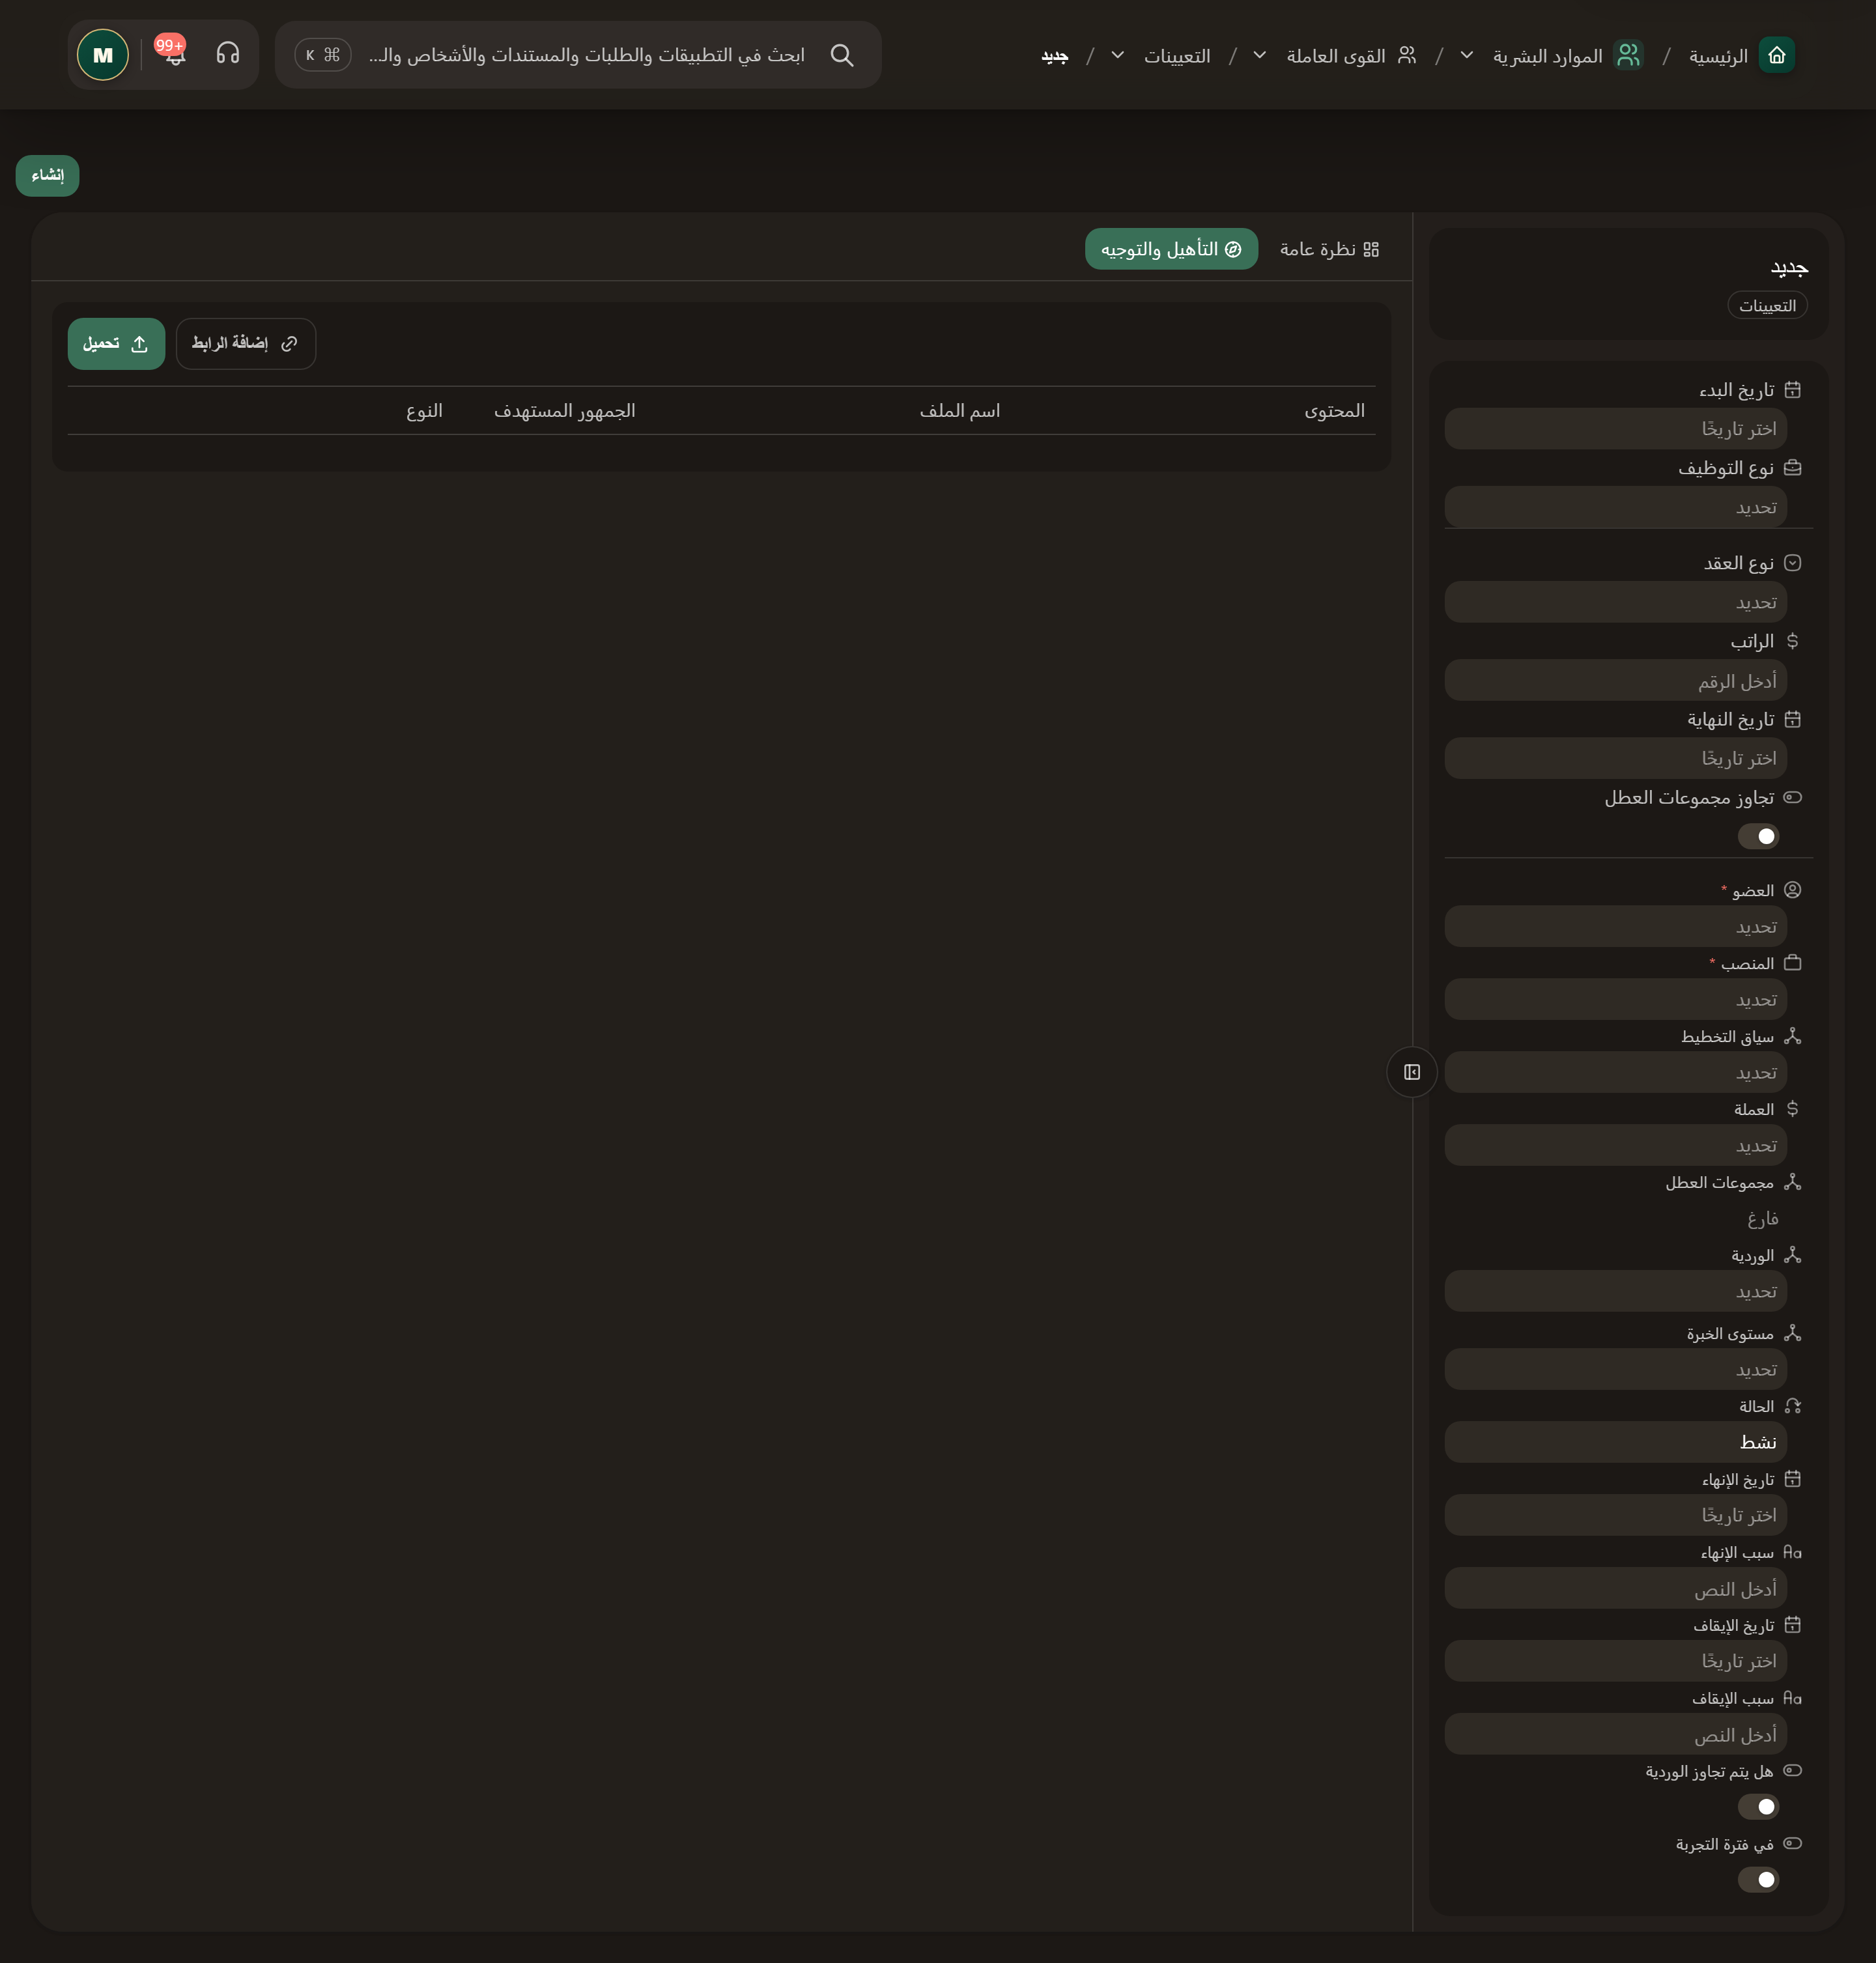
\includegraphics[width=0.95\linewidth]{figures/screens/ch02-assignment-fields-tab2-ar.png}
\caption{تبويب «التأهيل والتوجيه» كاملاً؛ نموذج غير محفوظ}
\label{fig:hr-assignments-fulltab1}
\end{figure}

\clearpage
\section{الوحدات التنظيمية}
\label{sec:hr-feature-nodes}

الوحدة التنظيمية قسم أو إدارة. حقل «يتبع ل» يضعها في شجرة الهيكل. وهي تحدد الجهة التي تتبعها الوظيفة، لا مكان العمل.

\textbf{متى تفيد؟} توضح الهيكل مع توسع الفريق. في شركة الأفق، تتبع الموارد البشرية الإدارة العامة. \textbf{المسار:} «الموارد البشرية» / «الأساسية» / «الوحدات التنظيمية».

\begin{figure}[H]
\centering
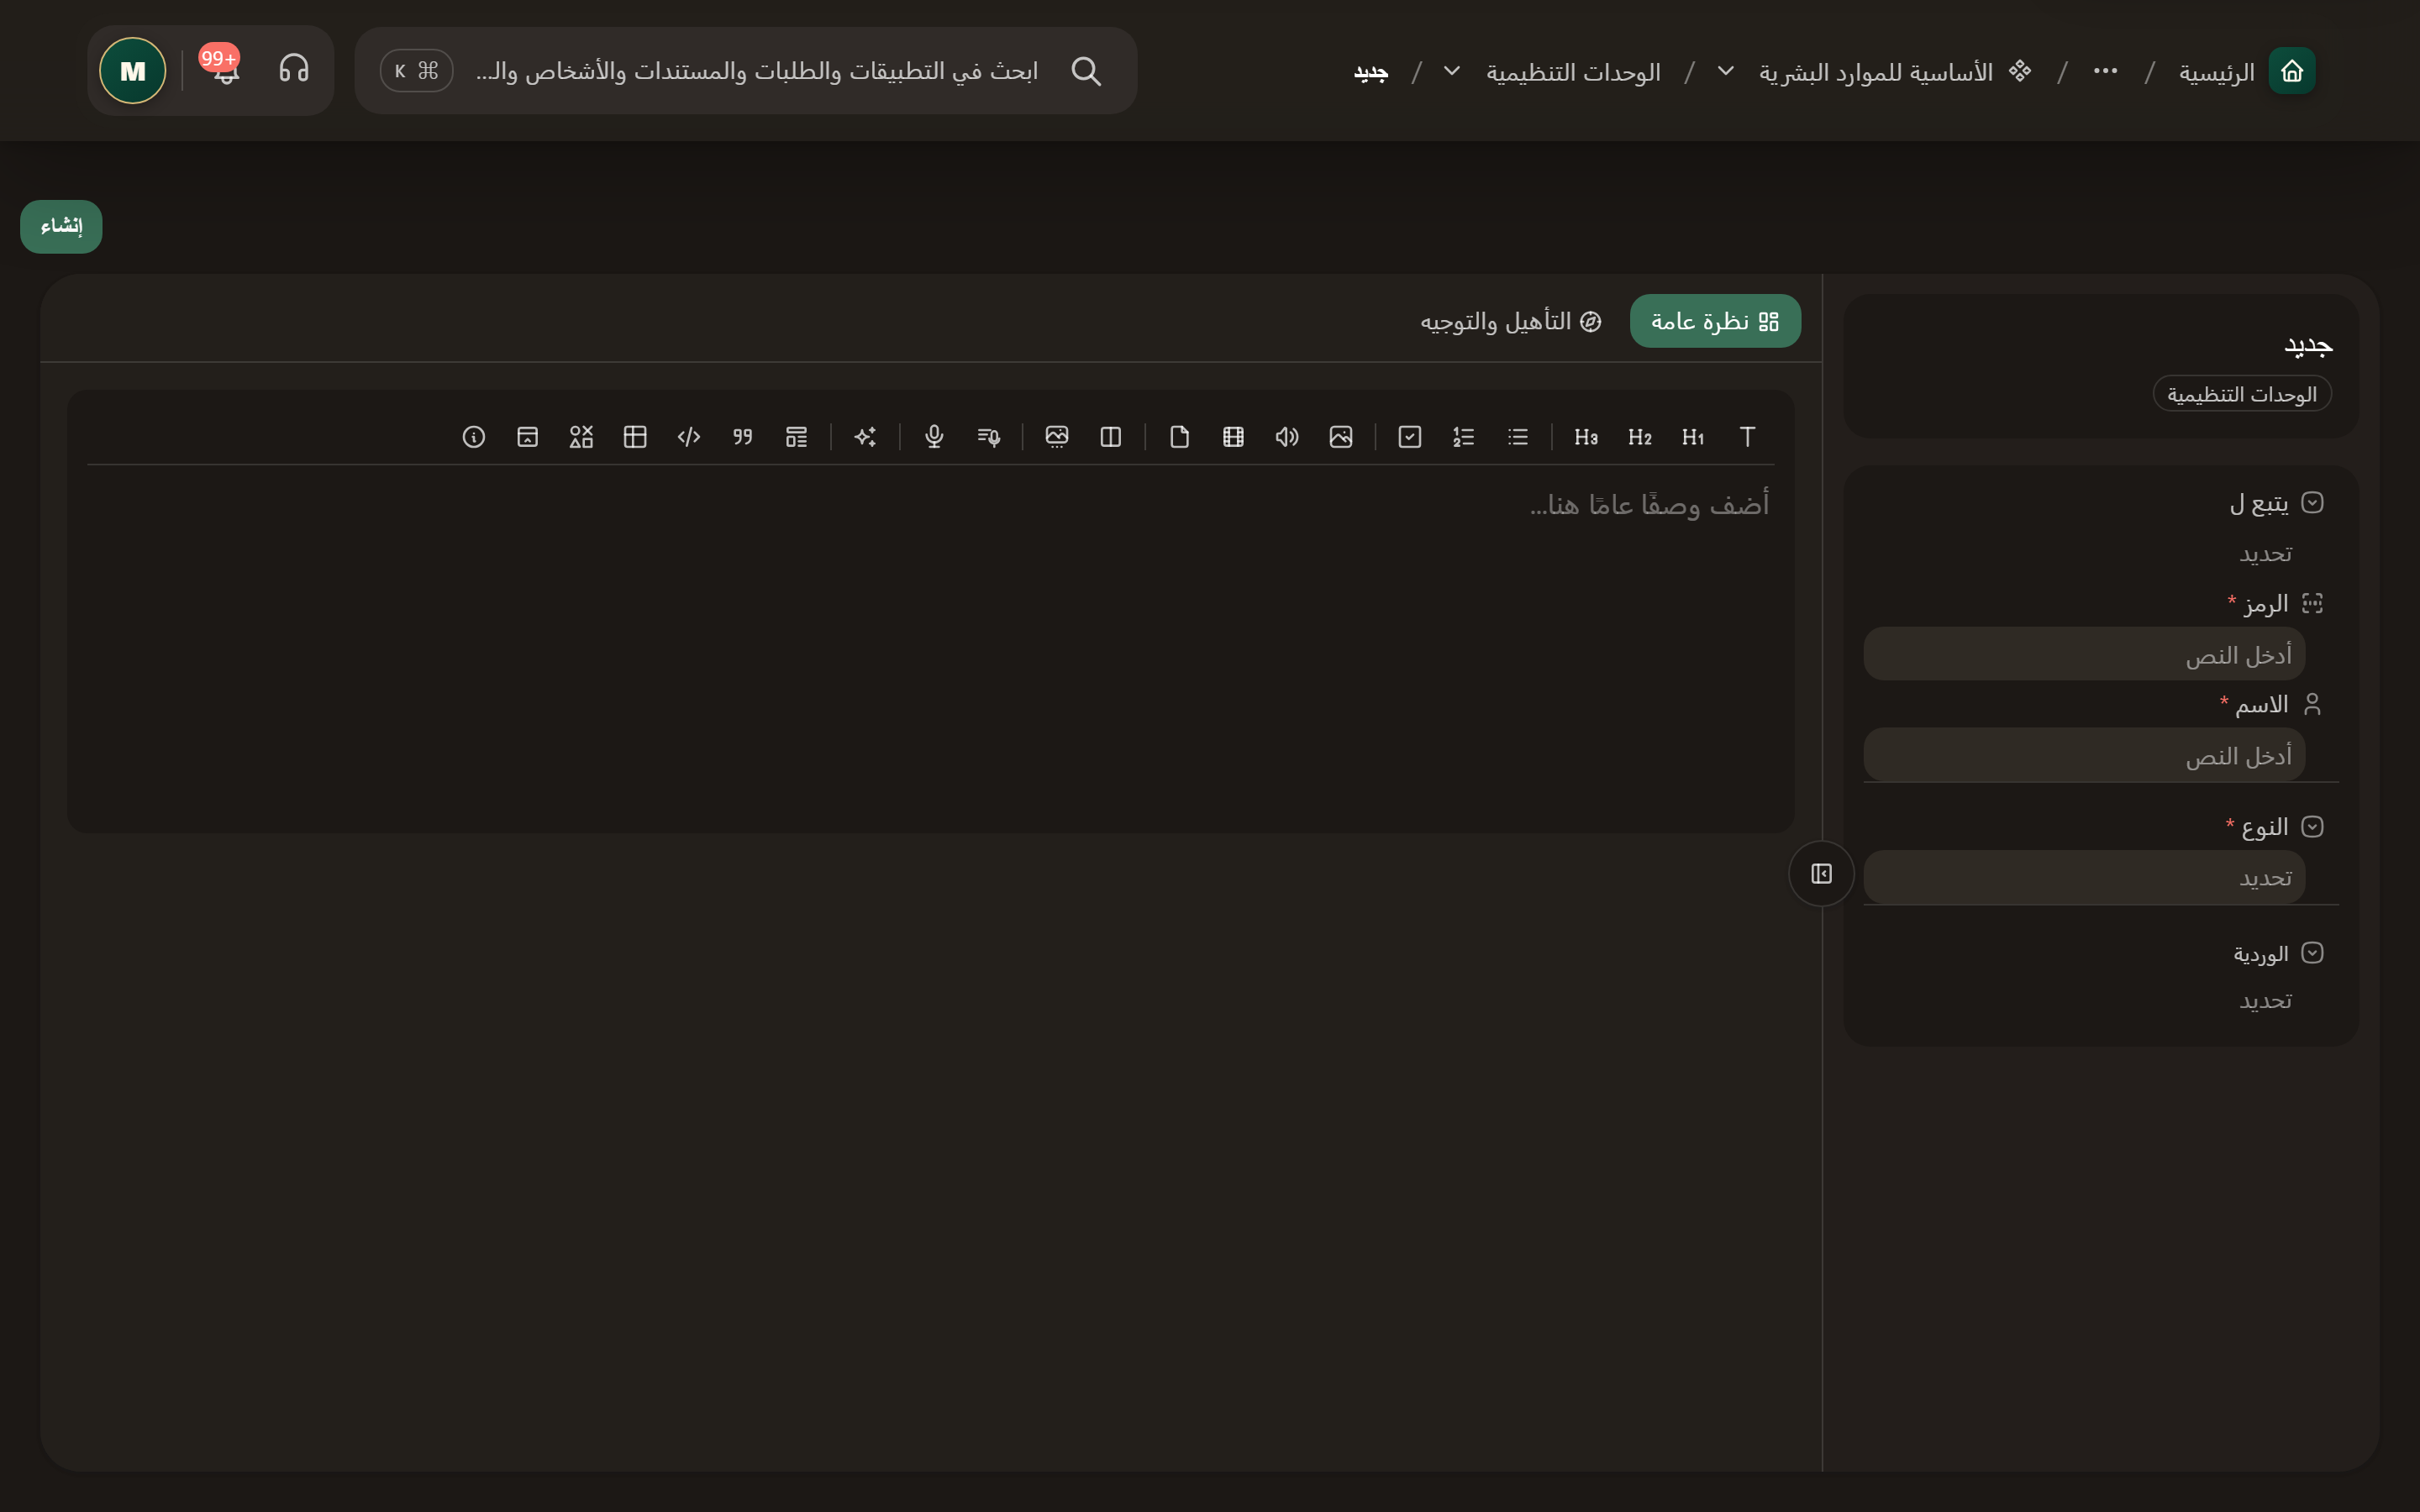
\includegraphics[width=0.95\linewidth]{figures/screens/ch02-node-fields-ar.png}
\caption{الوحدات التنظيمية: نموذج من بيئة الاختبار؛ لم يُحفظ}
\label{fig:hr-feature-nodes-screen}
\end{figure}

\begin{table}[H]
\centering
\caption{ما الذي تسجله في الوحدة؟}
\label{tab:hr-feature-nodes-data}
\rcZebra
\begin{tabularx}{\linewidth}{R{3.6cm} Y}
\rcHeaderRow
\thh{الحقل} & \thh{ما الذي تضيفه؟}\\
الرمز والاسم والنوع & \req{}؛ الأنواع يعرّفها مسؤول المؤسسة، مثل إدارة أو قسم.\\
يتبع ل & الوحدة الأم، مثل \en{HZN-GM} للموارد البشرية.\\
الوردية & تُورث من الوحدة الأم، أو تُستبدل بها وردية خاصة.\\
نظرة عامة والتأهيل والتوجيه & وصف الوحدة، ومواد تعريف الموظف الجديد بها.\\
\end{tabularx}
\end{table}

\subsection{ما الذي يمكنك فعله؟}

\begin{itemize}
  \item عرض «شجرة» مع البحث؛ كل بطاقة تبين المناصب والموظفين والشواغر.
  \item «مع الفروع» أو «بدون الفروع»: لتحديد إن كانت الأعداد تشمل الوحدات التابعة.
  \item «تجاوز» لاستبدال الوردية الموروثة، و«إعادة تعيين» لاستعادتها.
\end{itemize}

\begin{figure}[H]
\centering
\begin{tikzpicture}[node distance=0.5cm,stepBox/.append style={minimum width=6.5cm,text width=6.1cm,minimum height=0.8cm}]
  \node[stepBox] (a) {\RL{إنشاء الإدارة العامة}};
  \node[stepBox,below=of a] (b) {\RL{إضافة الموارد البشرية}\\\RL{تحتها}};
  \node[stepBox,below=of b] (c) {\RL{ربط منصب مدير الموارد}\\\RL{البشرية}};
  \draw[flowsTo] (a) -- (b);
  \draw[flowsTo] (b) -- (c);
\end{tikzpicture}
\rclegend
\caption{خطوات الاستخدام؛ الأسهم لا تعني معالجة تلقائية}
\label{fig:hr-feature-nodes-flow}
\end{figure}

\subsection{جرّب وراجع}

\begin{enumerate}
  \item افتح «الوحدات التنظيمية». إن لم تكن الإدارة العامة موجودة، أضفها برمز \en{HZN-GM} واختر نوعها ثم احفظ.
  \item أضف «الموارد البشرية» برمز \en{HZN-HR}، واختر النوع، والإدارة العامة في «يتبع ل»، ثم احفظ.
\end{enumerate}

\textbf{تحقق:} افتح الشجرة وتأكد أن الموارد البشرية تحت الإدارة العامة. ربط المنصب بالوحدة اختياري ولا يغني عن تعيين سارة.

\begin{figure}[H]
\centering
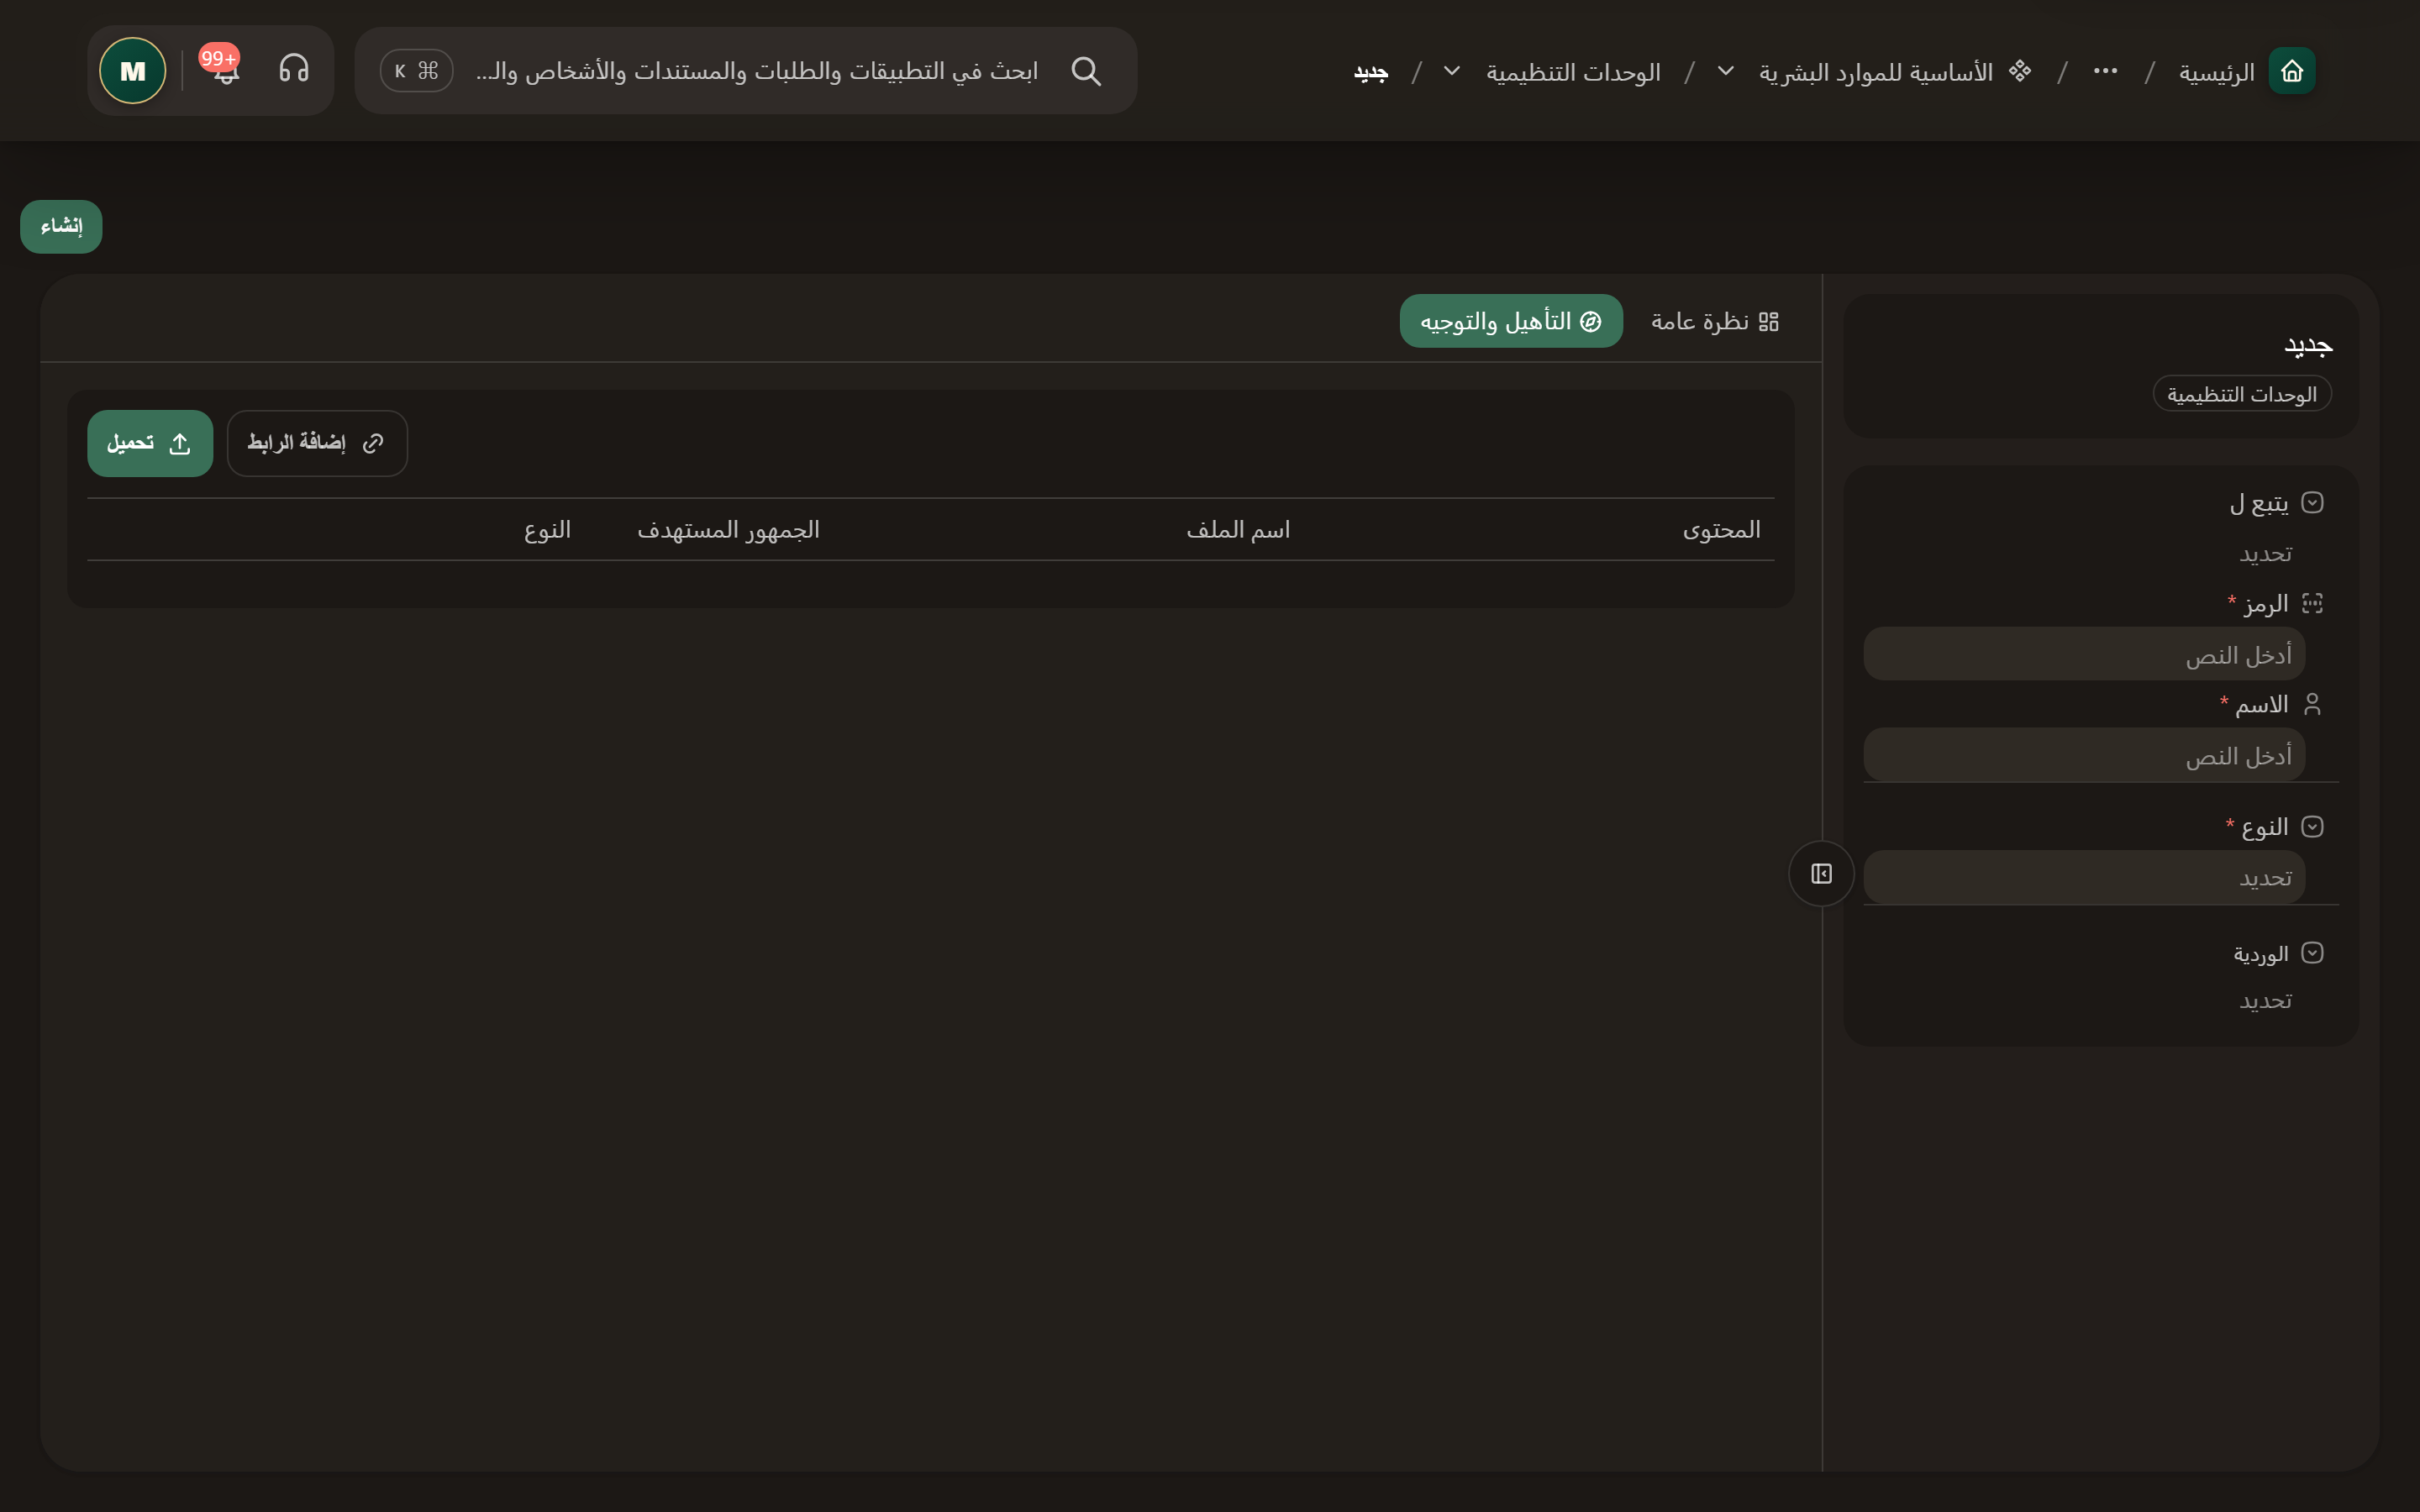
\includegraphics[width=0.95\linewidth]{figures/screens/ch02-node-fields-tab2-ar.png}
\caption{تبويب «التأهيل والتوجيه» كاملاً؛ نموذج غير محفوظ}
\label{fig:hr-nodes-fulltab1}
\end{figure}

\clearpage
\section{النقاط الجغرافية}
\label{sec:hr-feature-locations}

النقطة الجغرافية مكان عمل، مثل مكتب أو فرع، بعنوانه ونقطته على الخريطة. ويمكن أن يتبع موقعاً آخر.

\textbf{متى تفيد؟} تفصل المكان عن القسم: قسمان في مقر دمشق، أو قسم واحد في عدة مواقع. \textbf{المسار:} «الموارد البشرية» / «الأساسية» / «النقاط الجغرافية».

\begin{figure}[H]
\centering
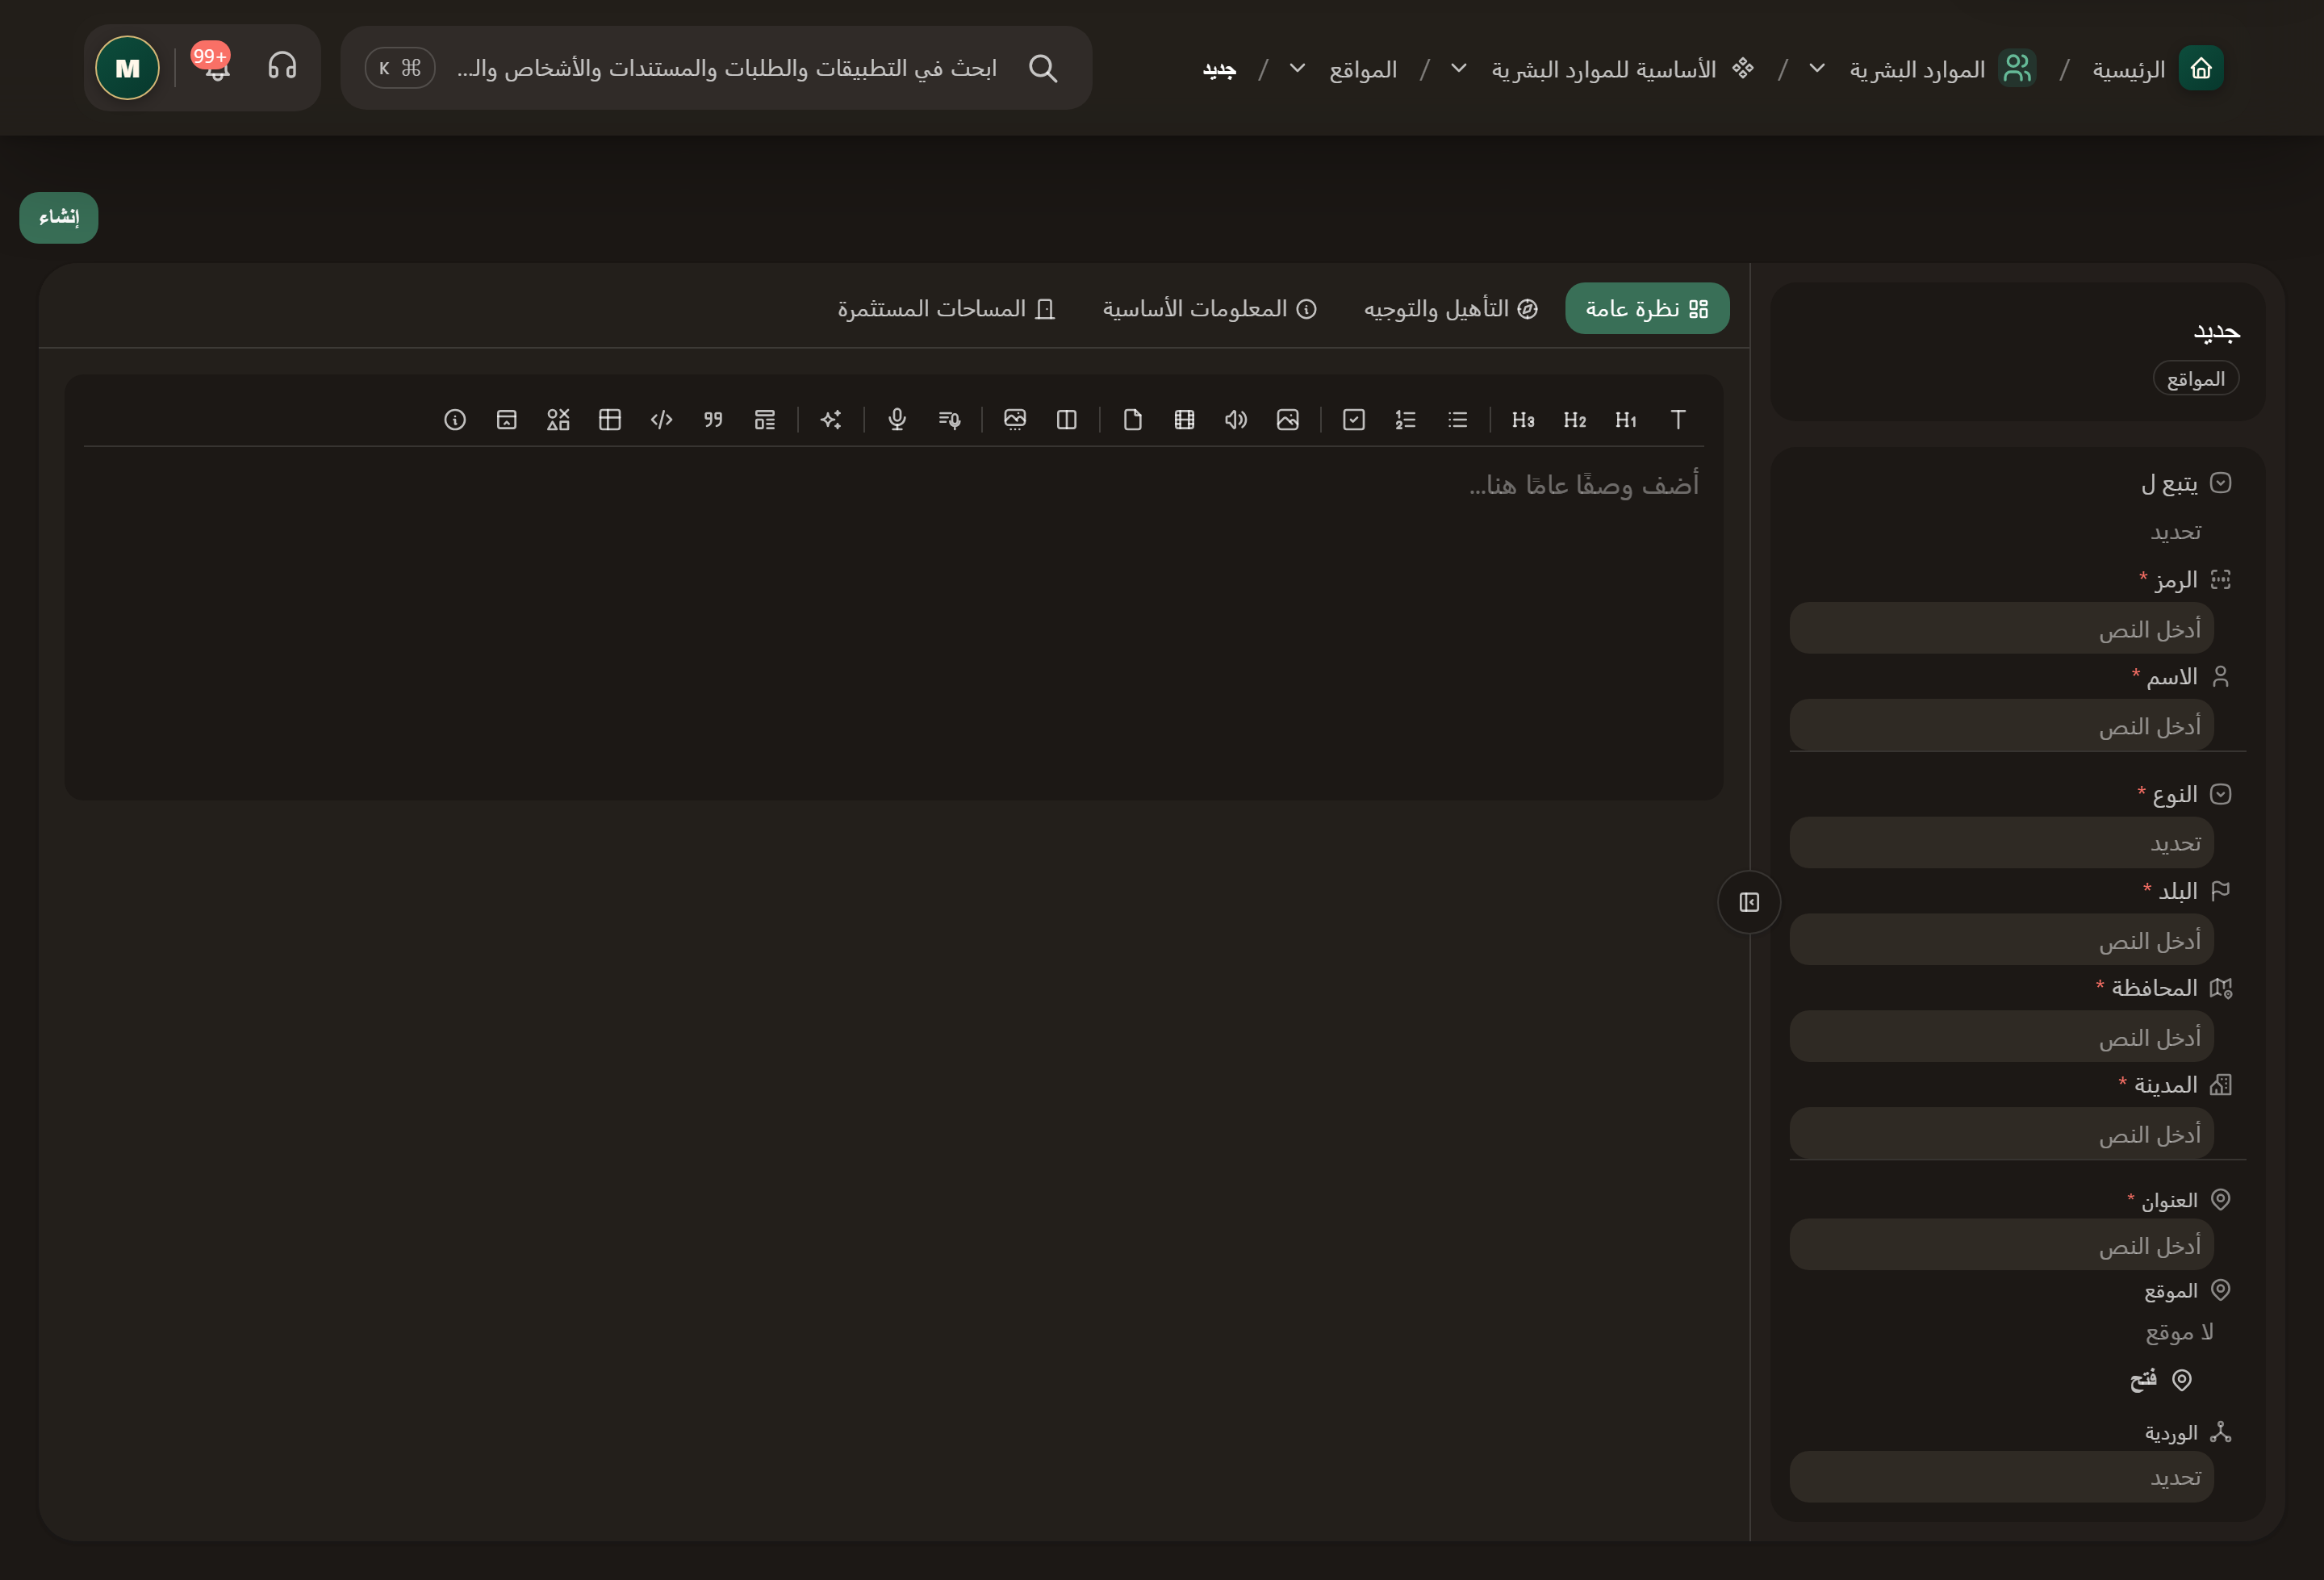
\includegraphics[width=0.95\linewidth]{figures/screens/ch02-location-fields-ar.png}
\caption{النقاط الجغرافية: نموذج من بيئة الاختبار؛ لم يُحفظ}
\label{fig:hr-feature-locations-screen}
\end{figure}

\begin{table}[H]
\centering
\caption{ما الذي تسجله في الموقع؟}
\label{tab:hr-feature-locations-data}
\rcZebra
\begin{tabularx}{\linewidth}{R{3.6cm} Y}
\rcHeaderRow
\thh{التبويب أو الحقل} & \thh{ما الذي تضيفه؟}\\
الأساسية & الرمز والاسم والنوع \req{}؛ الموقع الأم والوردية \opt{}.\\
العنوان & البلد والمحافظة والمدينة والعنوان \req{}، ونقطة على الخريطة.\\
المعلومات الأساسية & الملكية، المساحة بالمتر المربع، ملف العقد.\\
المساحات المستثمرة & الغرف: النوع والرمز والطابق والسعة والمساحة، والتجهيزات مثل الشاشة وجهاز العرض.\\
\end{tabularx}
\end{table}

\subsection{ما الذي يمكنك فعله؟}

\begin{itemize}
  \item عرض «خريطة» تُظهر المواقع بدبابيس، أو «شجرة» تُظهر المواقع وتوابعها.
  \item البحث بالاسم أو الرمز أو المدينة أو العنوان، والتصفية بالنوع والبلد.
\end{itemize}

\begin{figure}[H]
\centering
\begin{tikzpicture}[node distance=0.5cm,stepBox/.append style={minimum width=6.5cm,text width=6.1cm,minimum height=0.8cm}]
  \node[stepBox] (a) {\RL{تعريف مكان العمل}};
  \node[stepBox,below=of a] (b) {\RL{مراجعة العنوان}};
  \node[stepBox,below=of b] (c) {\RL{ربط المنصب}};
  \draw[flowsTo] (a) -- (b);
  \draw[flowsTo] (b) -- (c);
\end{tikzpicture}
\rclegend
\caption{خطوات الاستخدام؛ الأسهم لا تعني معالجة تلقائية}
\label{fig:hr-feature-locations-flow}
\end{figure}

\subsection{جرّب وراجع}

\begin{enumerate}
  \item افتح «النقاط الجغرافية» وابحث عن المقر الرئيسي بدمشق.
  \item إن لم يكن موجوداً، أضف \en{HZN-DAM} مع الاسم والنوع والبلد والمحافظة والمدينة والعنوان، وحدد النقطة على الخريطة، ثم احفظ. لا تختر موقعاً أماً إلا إذا كان هذا الموقع يتبع موقعاً آخر.
\end{enumerate}

\textbf{تحقق:} افتح عرض الخريطة وتأكد من مكان الدبوس. اربط الموقع من صفحة المنصب؛ الموقع وحده لا يعيّن موظفاً.

\begin{figure}[H]
\centering
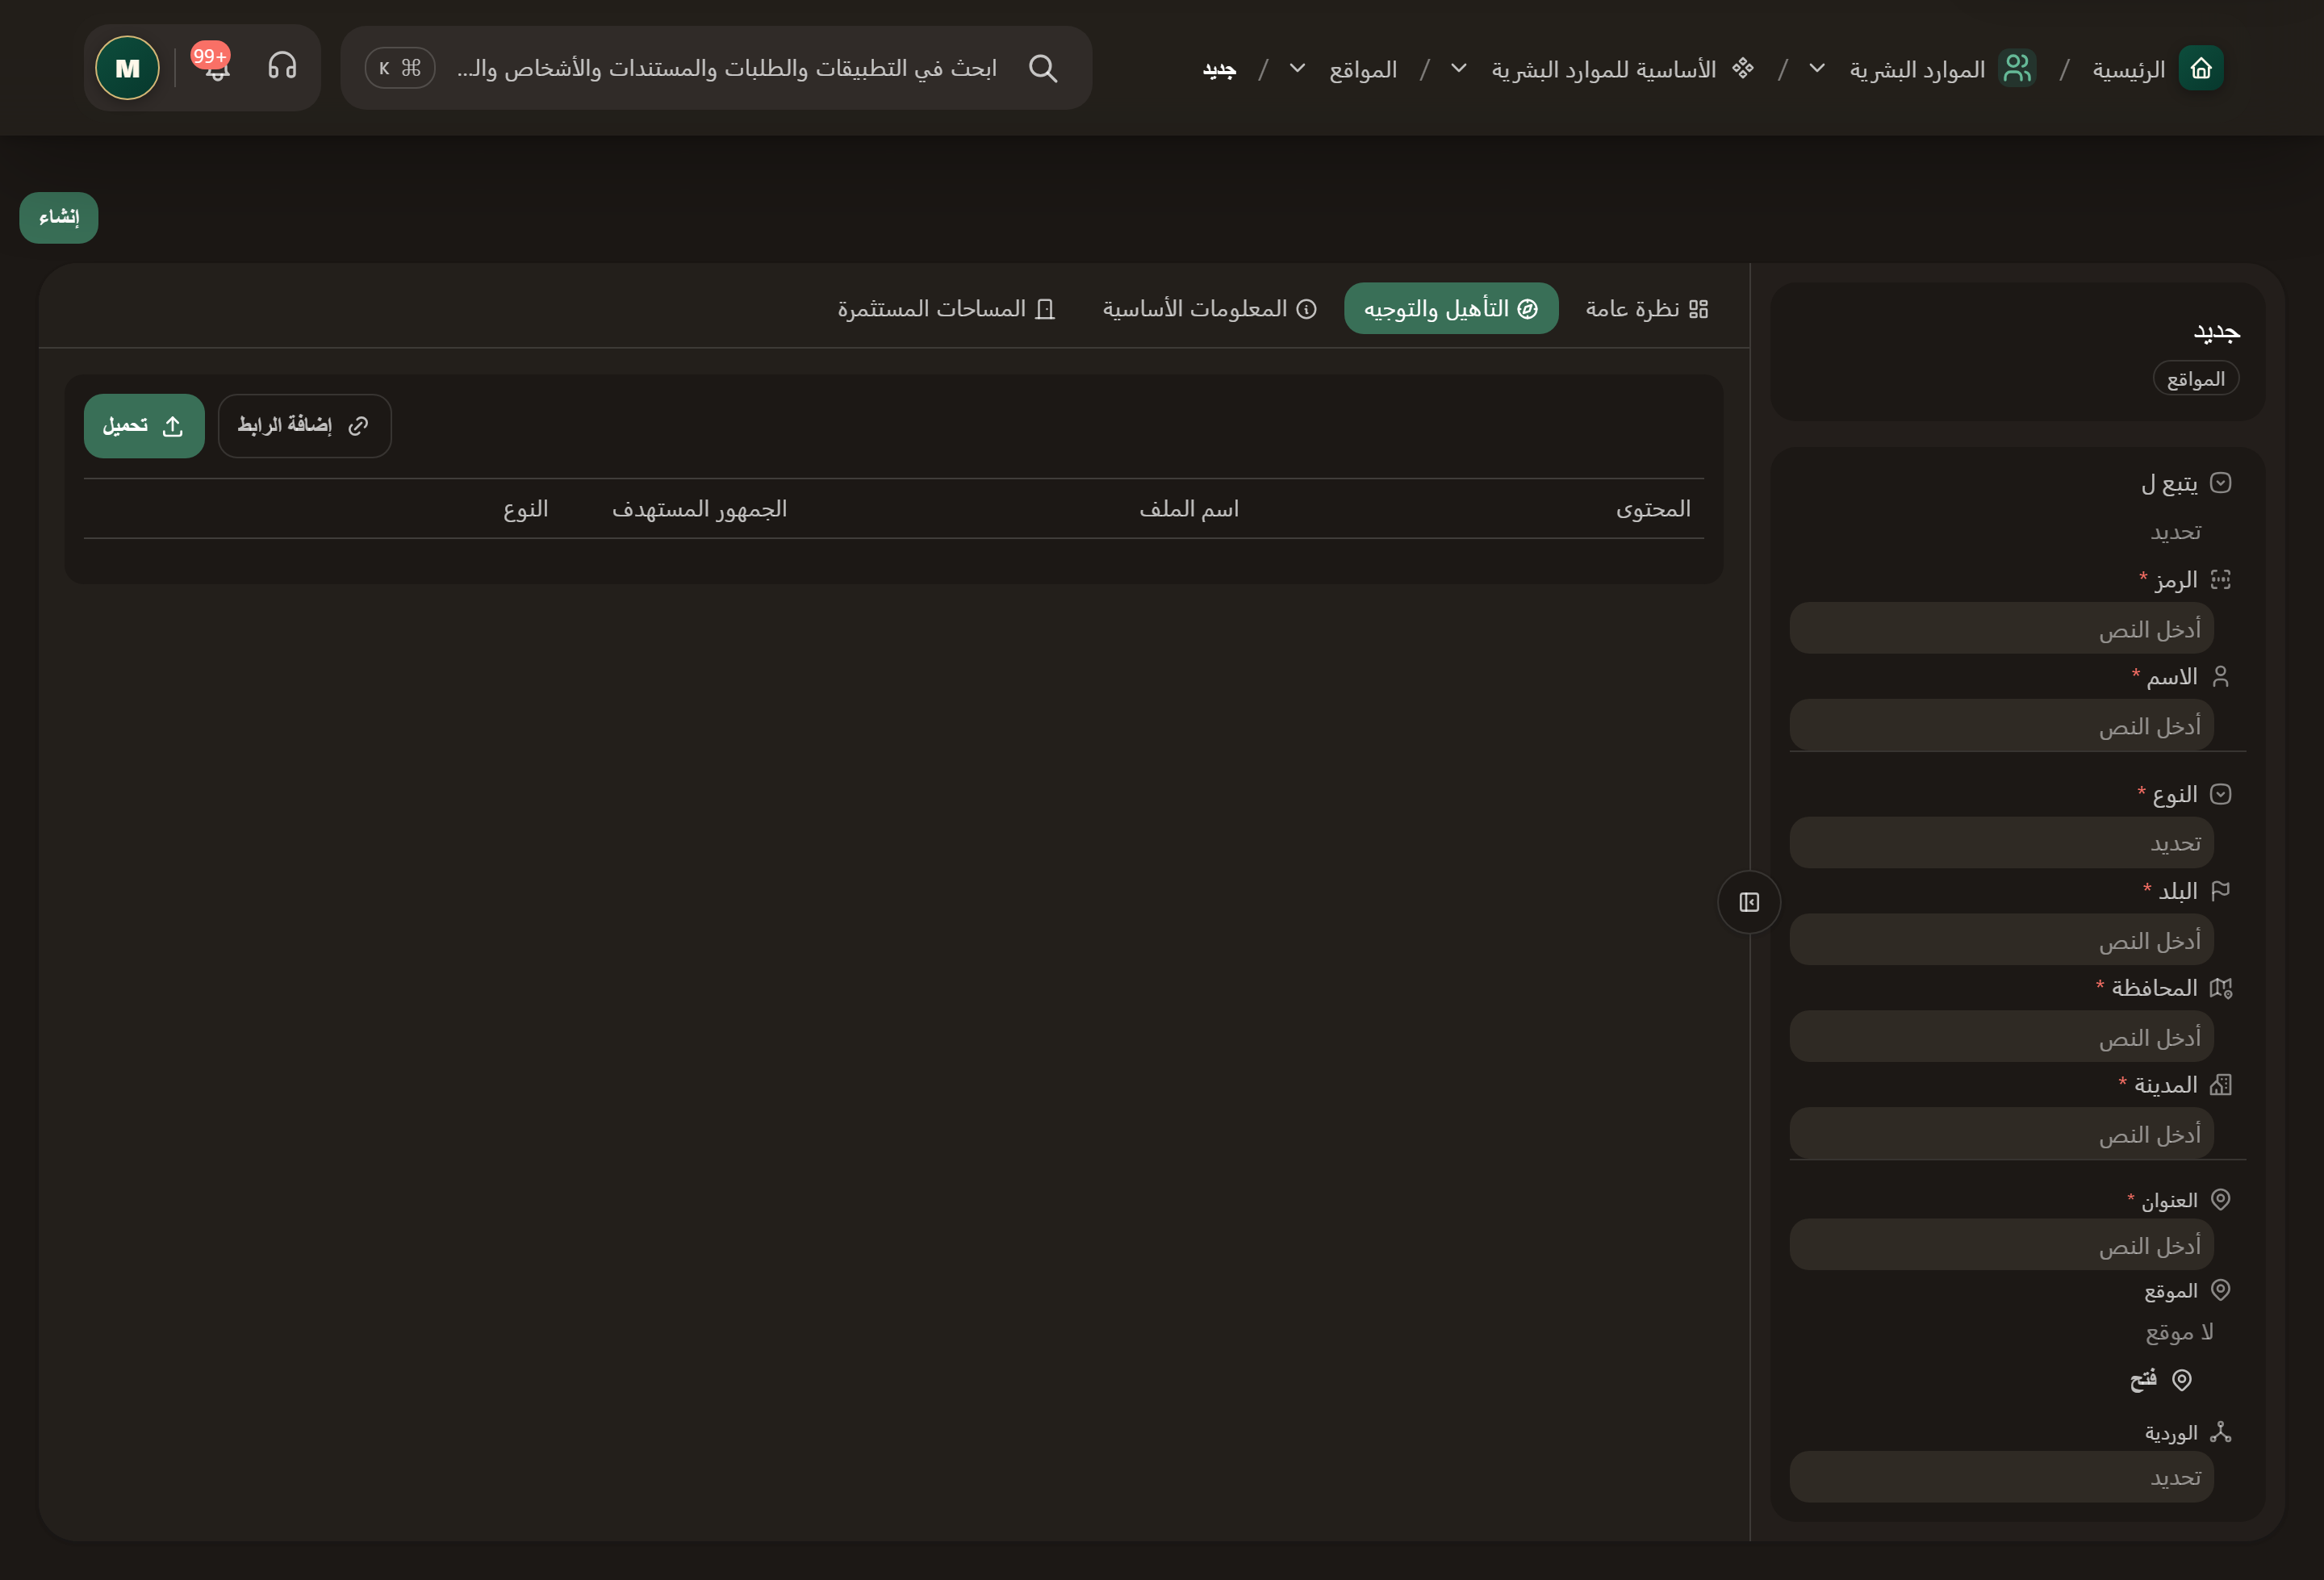
\includegraphics[width=0.95\linewidth]{figures/screens/ch02-location-fields-tab2-ar.png}
\caption{تبويب «التأهيل والتوجيه» كاملاً؛ نموذج غير محفوظ}
\label{fig:hr-locations-fulltab1}
\end{figure}

\begin{figure}[H]
\centering
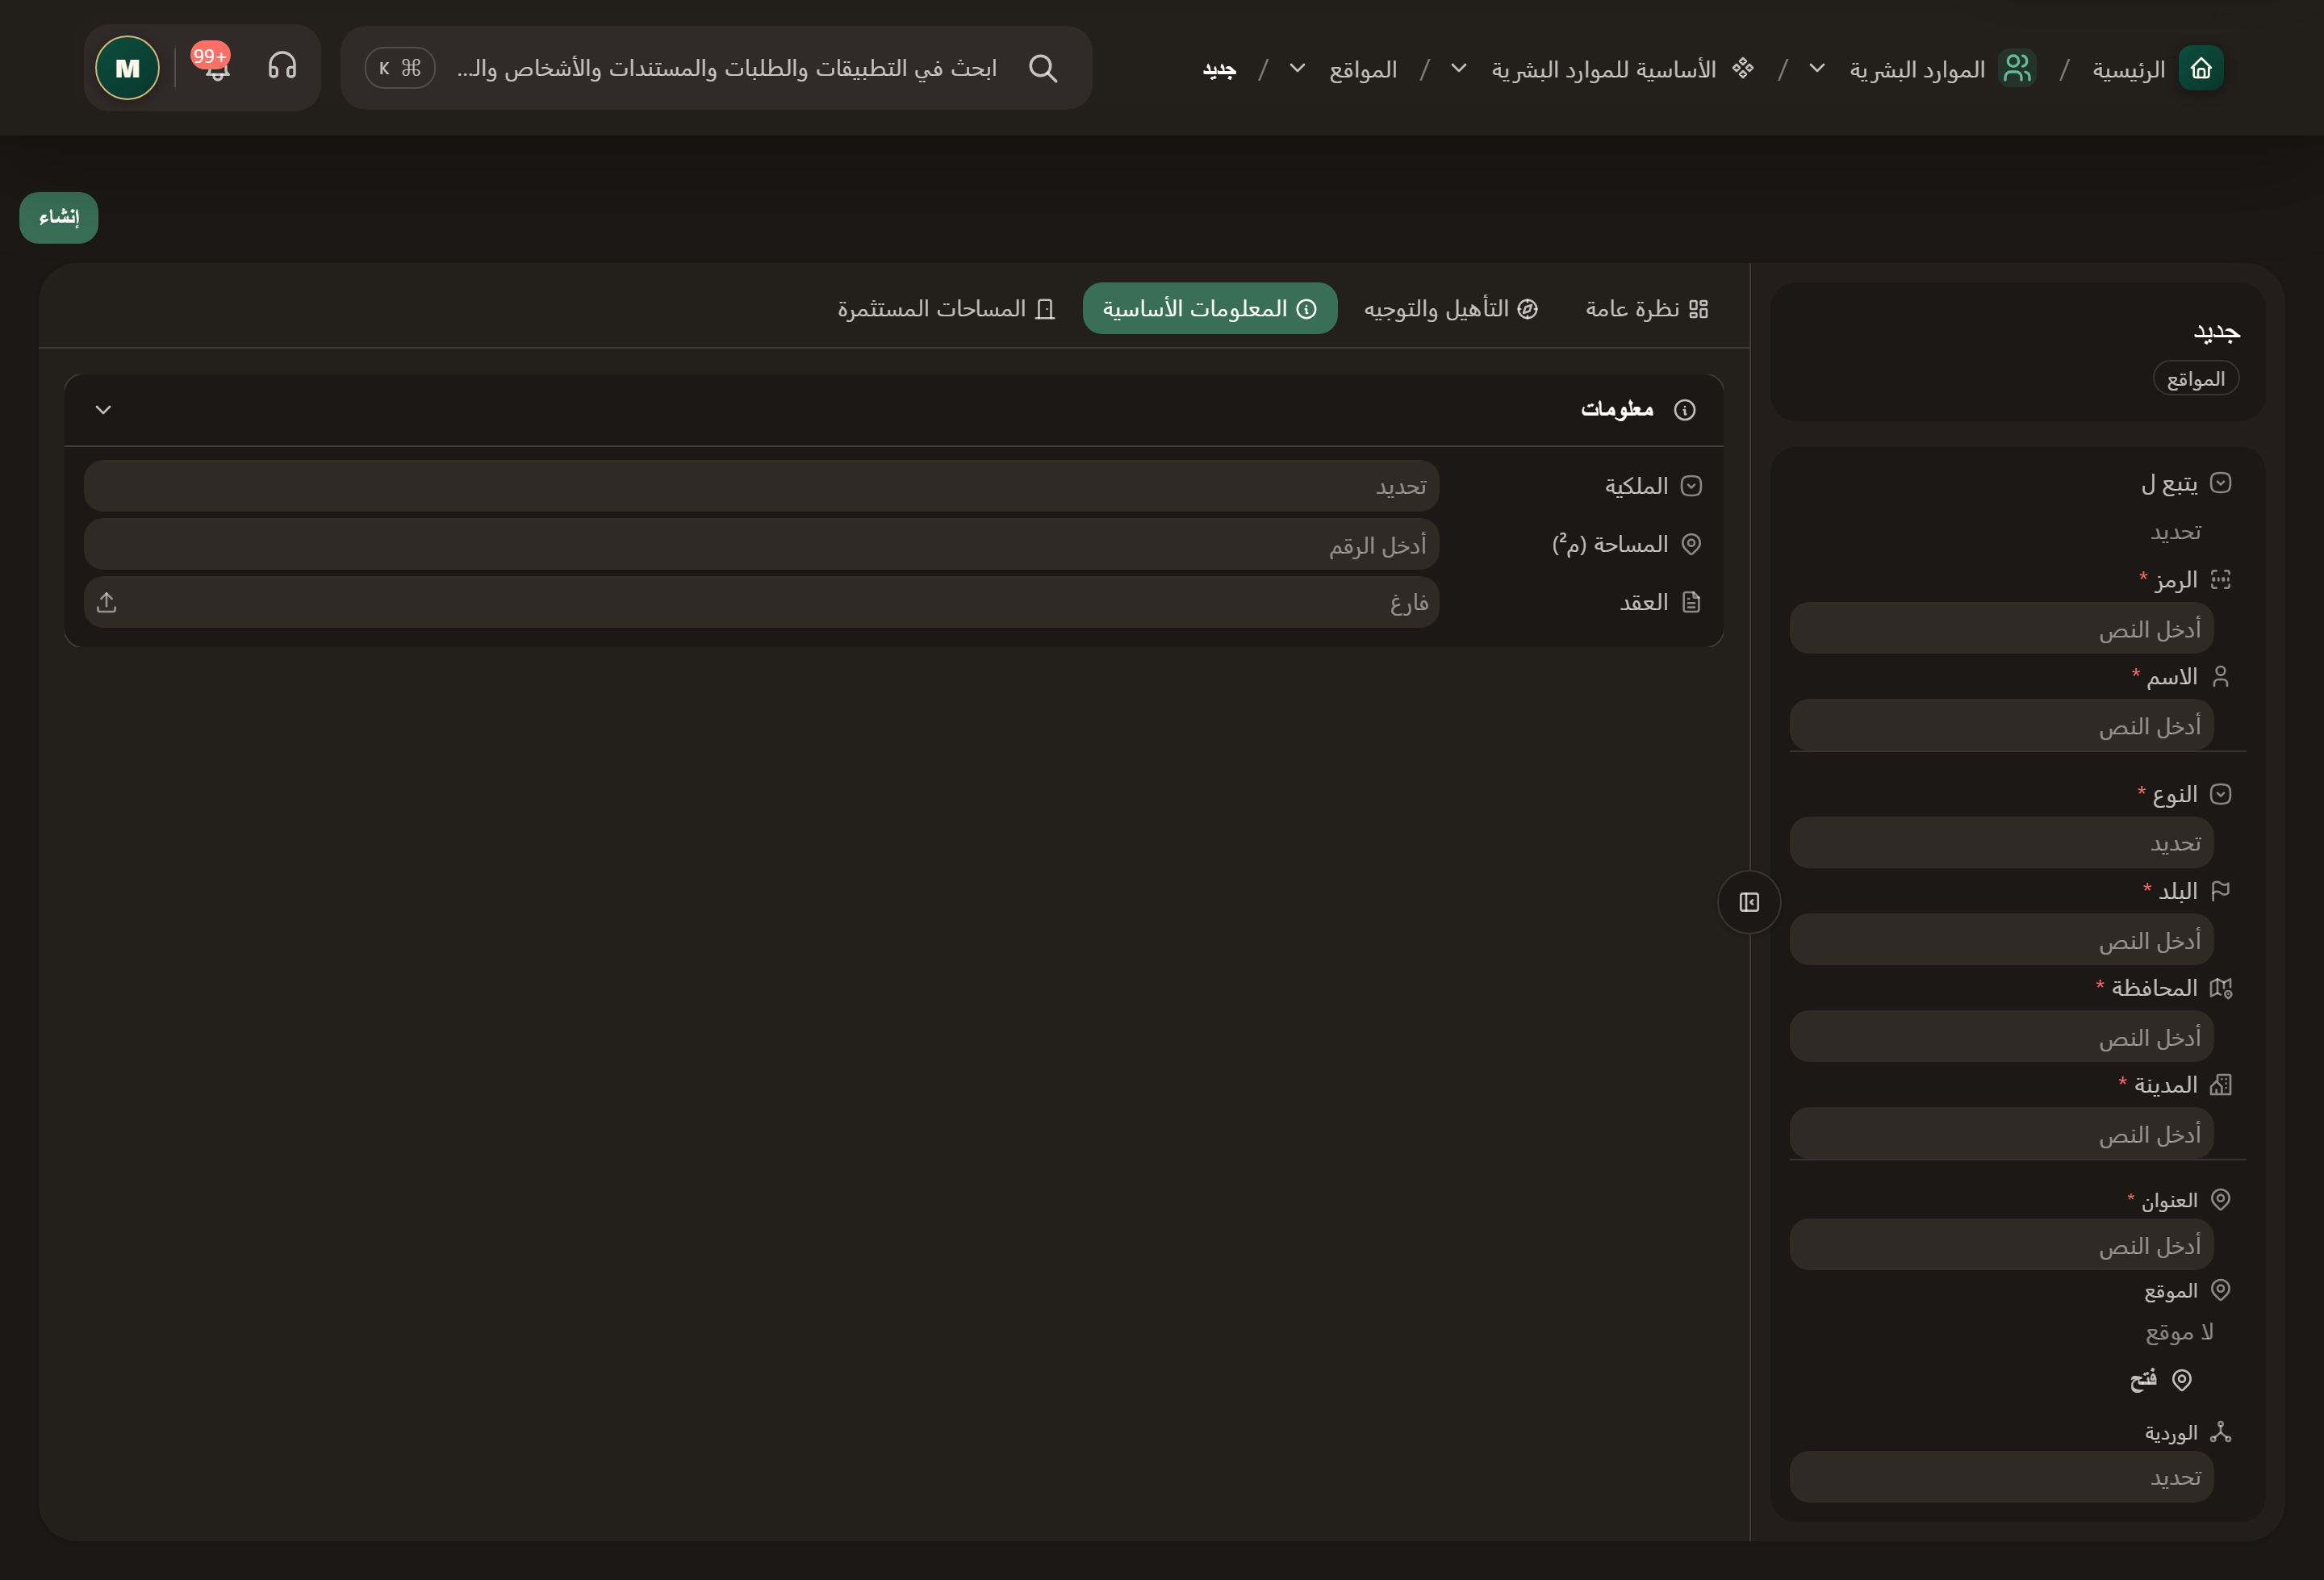
\includegraphics[width=0.95\linewidth]{figures/screens/ch02-location-fields-tab3-ar.png}
\caption{تبويب «المعلومات الأساسية» كاملاً؛ نموذج غير محفوظ}
\label{fig:hr-locations-fulltab2}
\end{figure}

\begin{figure}[H]
\centering
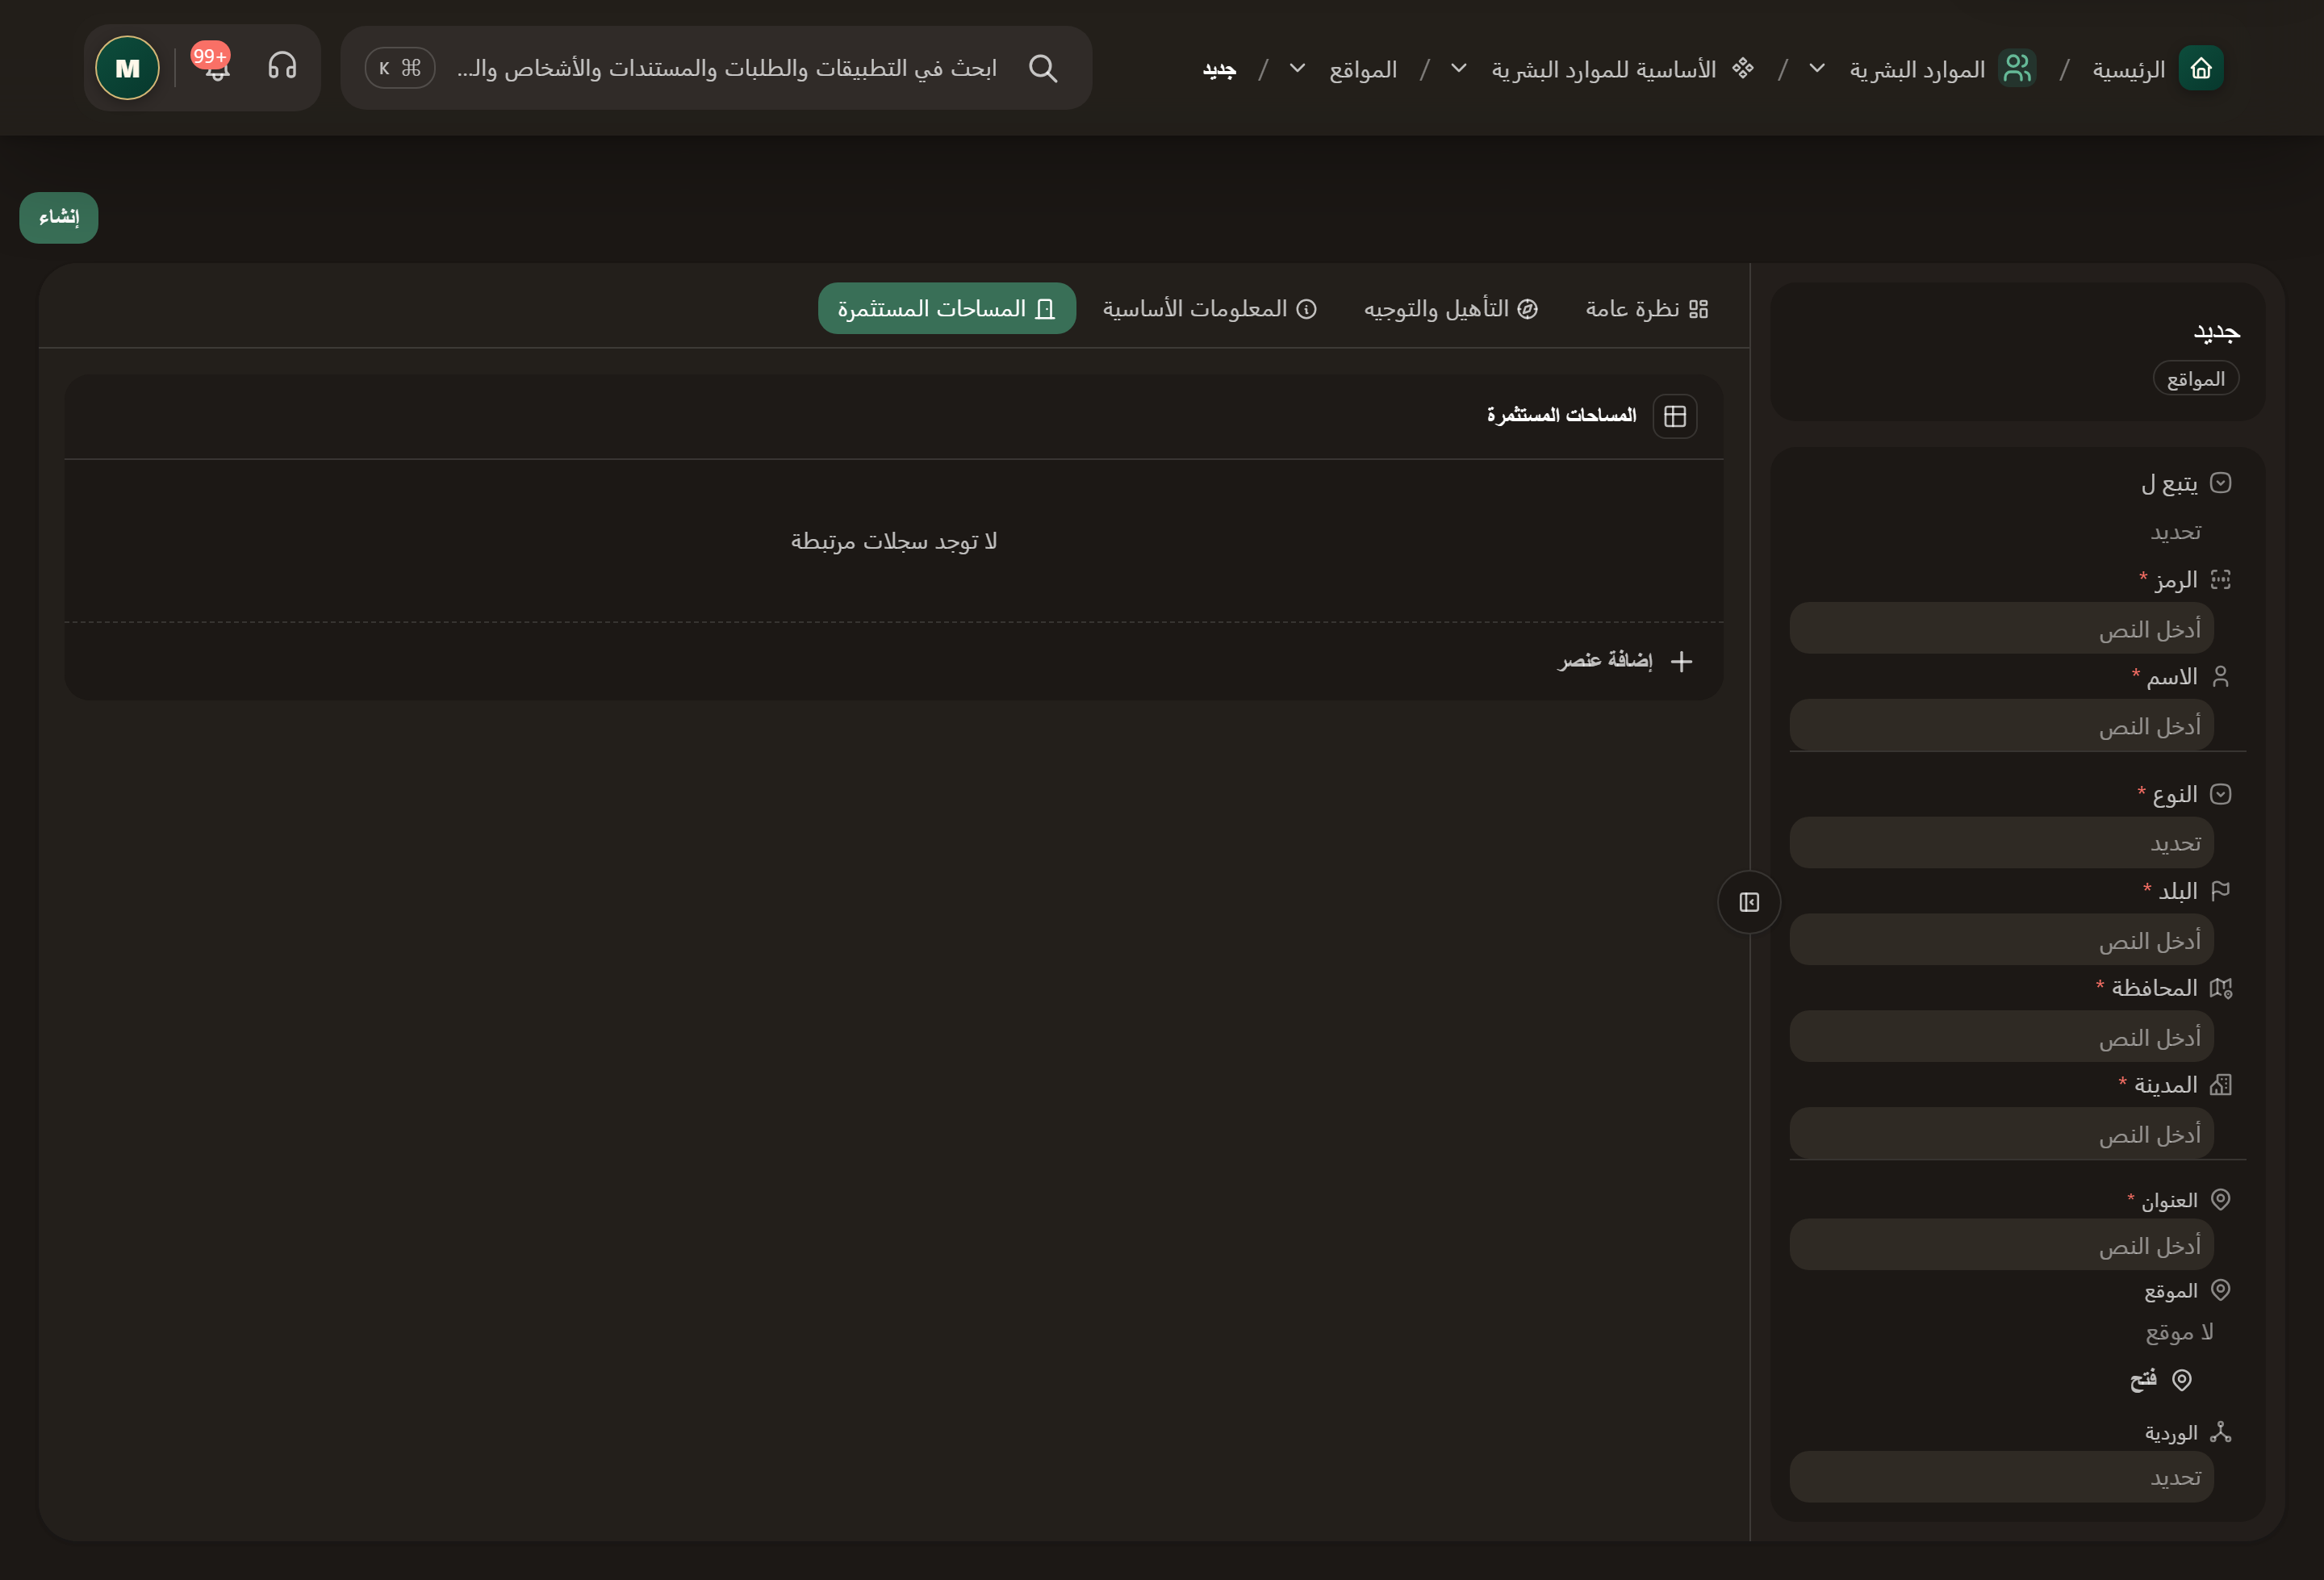
\includegraphics[width=0.95\linewidth]{figures/screens/ch02-location-fields-tab4-ar.png}
\caption{تبويب «المساحات المستثمرة» كاملاً؛ نموذج غير محفوظ}
\label{fig:hr-locations-fulltab3}
\end{figure}

\clearpage
\section{المجموعات}
\label{sec:hr-feature-groups}

المجموعة فريق أو لجنة تجمع أعضاء من أقسام مختلفة، دون تغيير وظائفهم.

\textbf{متى تفيد؟} مثلاً فريق تجهيز مكتب الأفق، أو لجنة تضم كل موظفي فرع حلب. \textbf{المسار:} «الموارد البشرية» / «القوى العاملة» / «المجموعات».

\begin{figure}[H]
\centering
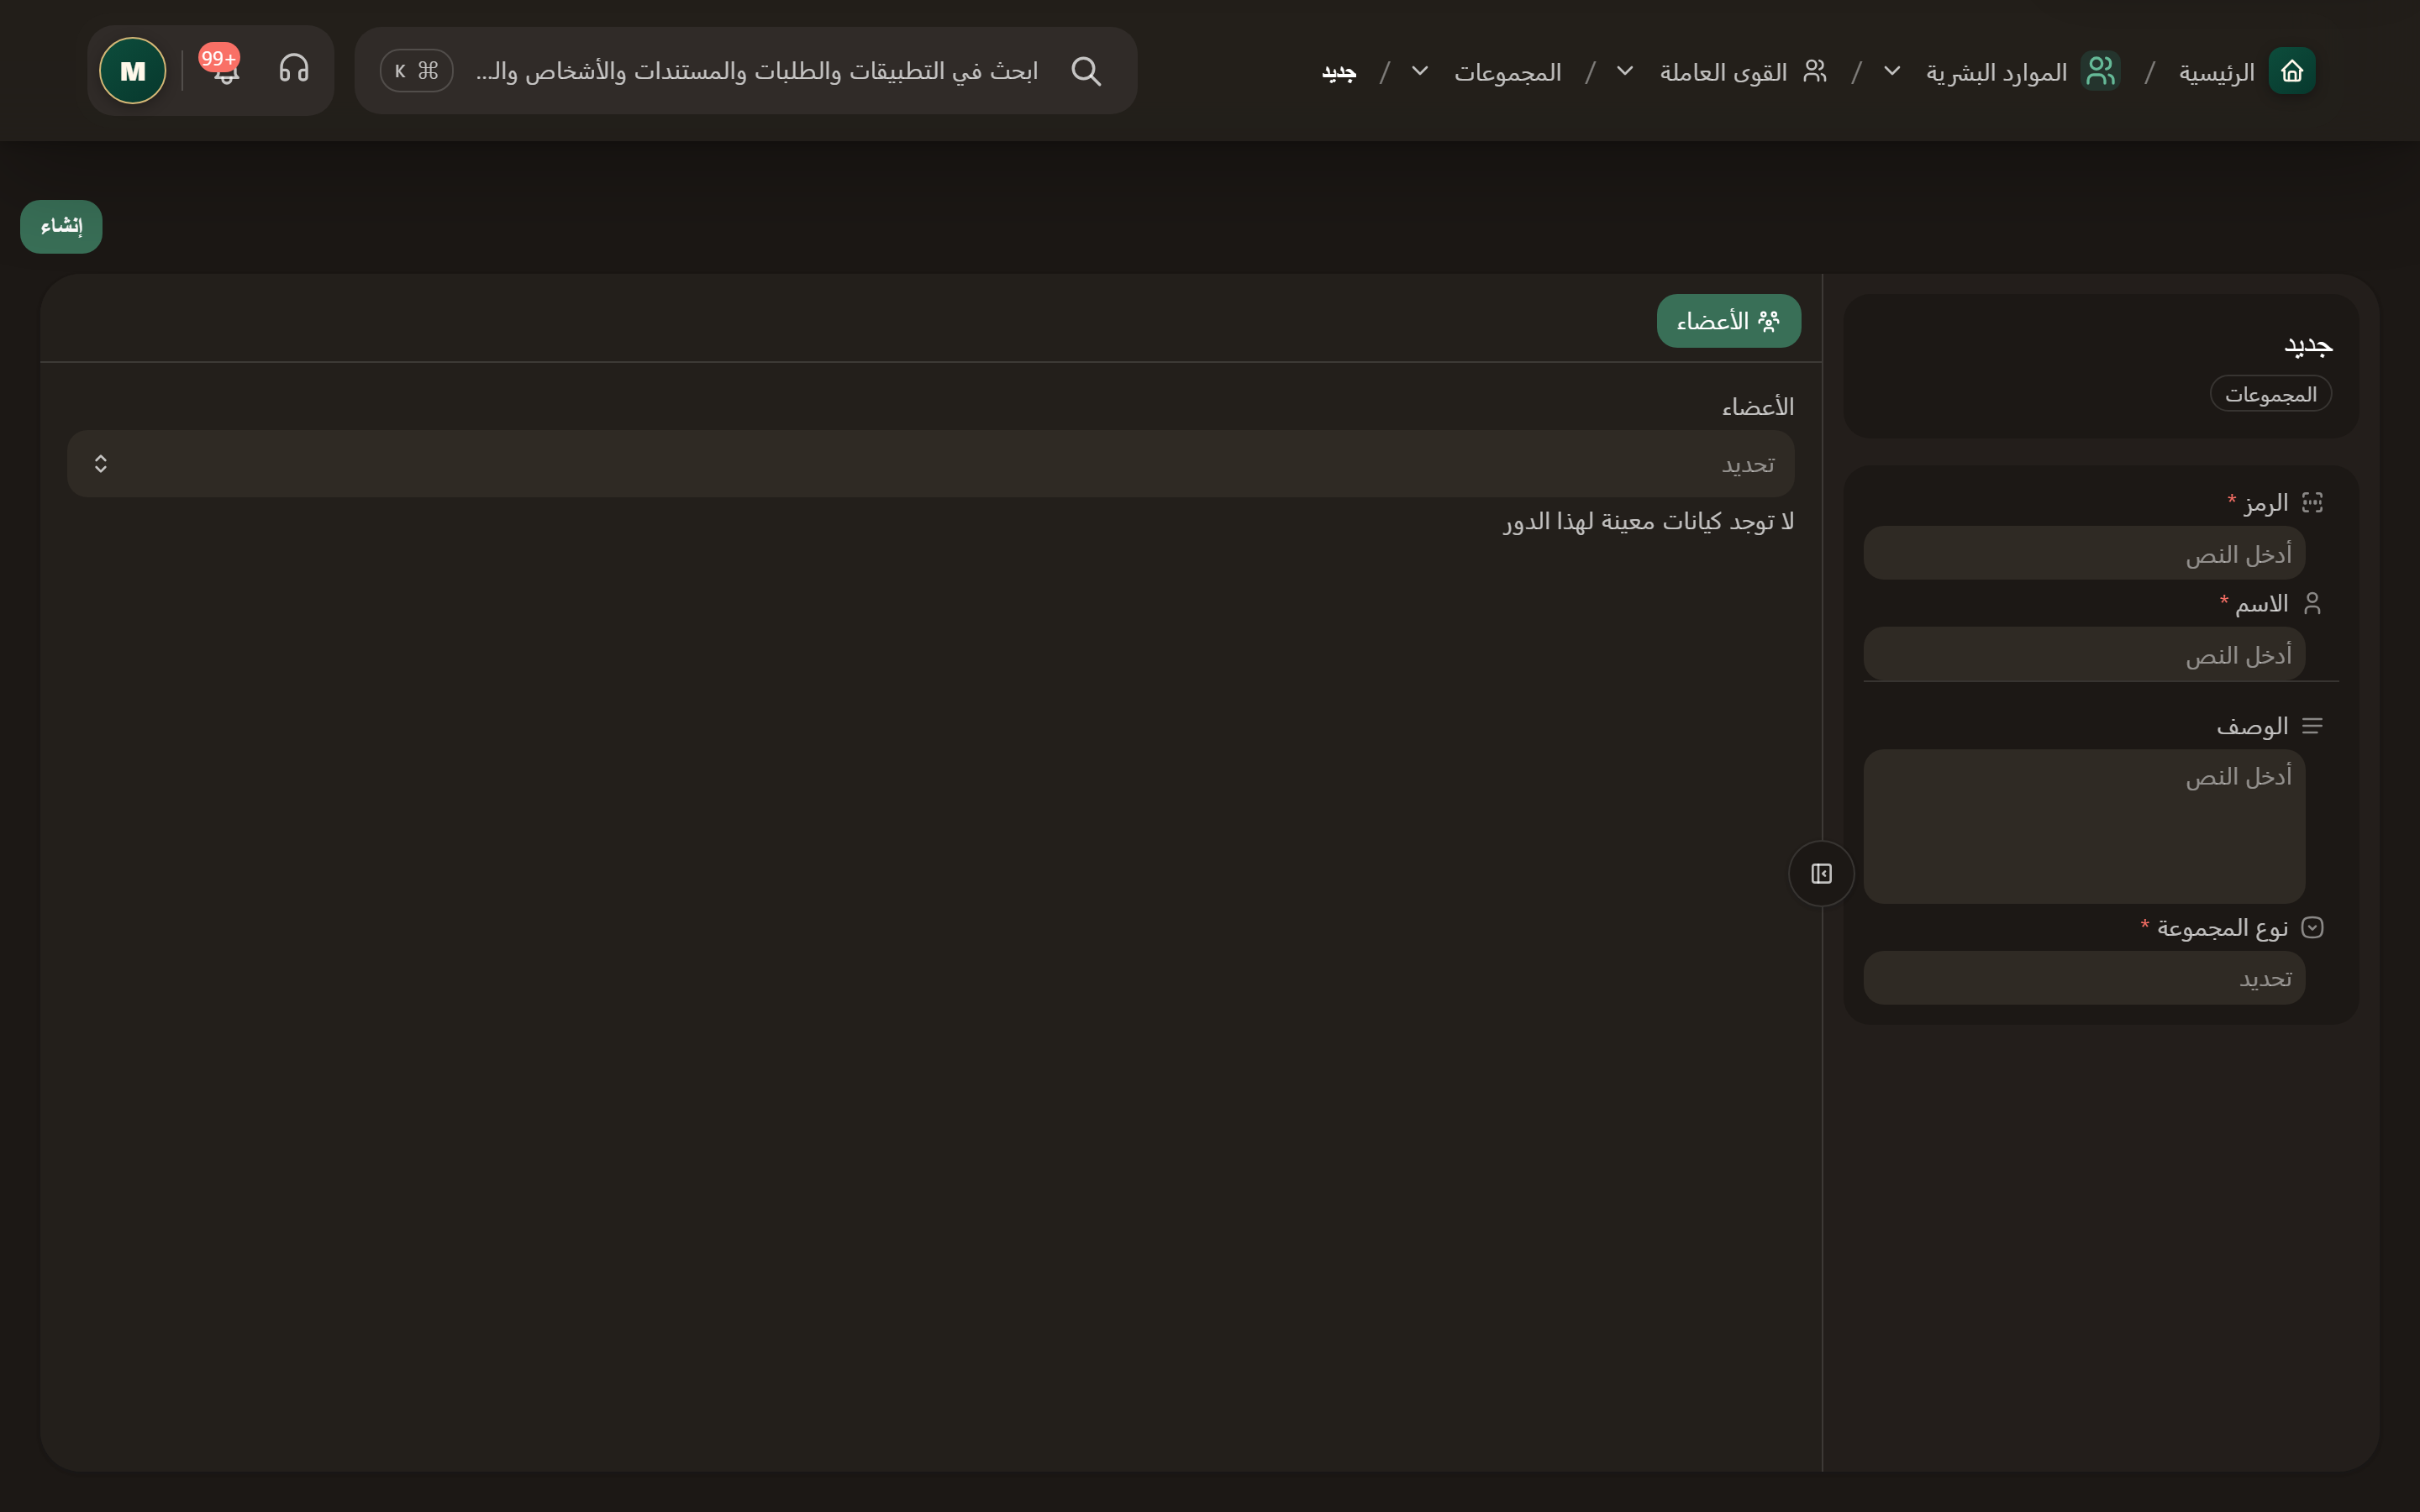
\includegraphics[width=0.95\linewidth]{figures/screens/ch03-feature-groups-ar.png}
\caption{المجموعات: نموذج غير محفوظ في بيئة الاختبار}
\label{fig:hr-feature-groups-screen}
\end{figure}

\begin{table}[H]
\centering
\caption{ما الذي تسجله في المجموعة؟}
\label{tab:hr-feature-groups-data}
\rcZebra
\begin{tabularx}{\linewidth}{R{3.6cm} Y}
\rcHeaderRow
\thh{التبويب أو الحقل} & \thh{ما الذي تضيفه؟}\\
الأساسية & الرمز والاسم \req{}، والوصف.\\
نوع المجموعة & \req{}: «يدوي» تختار أعضاءها بنفسك، أو «قائم على الكود» يحدد فيه شرطٌ الأعضاء ويحسبهم النظام \gen{}.\\
الأعضاء & أشخاص، أو كل من في قسم أو موقع أو منصب أو مجموعة، أو المؤسسة كلها.\\
حسابات البريد & صندوق بريد مشترك، أو قائمة بريدية للمجموعة.\\
\end{tabularx}
\end{table}

\begin{figure}[H]
\centering
\begin{tikzpicture}[node distance=0.5cm,stepBox/.append style={minimum width=6.5cm,text width=6.1cm,minimum height=0.8cm}]
  \node[stepBox] (a) {\RL{تحديد الفريق}};
  \node[stepBox,below=of a] (b) {\RL{اختيار طريقة العضوية}};
  \node[stepBox,below=of b] (c) {\RL{مراجعة الأعضاء}};
  \draw[flowsTo] (a) -- (b);
  \draw[flowsTo] (b) -- (c);
\end{tikzpicture}
\rclegend
\caption{خطوات الاستخدام؛ الأسهم لا تعني معالجة تلقائية}
\label{fig:hr-feature-groups-flow}
\end{figure}

\subsection{جرّب وراجع}

\begin{enumerate}
  \item افتح «المجموعات» وتأكد أن المجموعة غير موجودة.
  \item أضف رمزاً واسماً، واختر «يدوي»، ثم افتح «الأعضاء» واختر سارة وعمر، واحفظ.
\end{enumerate}

\textbf{تحقق:} أعد فتح المجموعة وراجع الأعضاء. انضمام سارة إلى المجموعة لا يغيّر تعيينها مديرةً للموارد البشرية.

\begin{figure}[H]
\centering
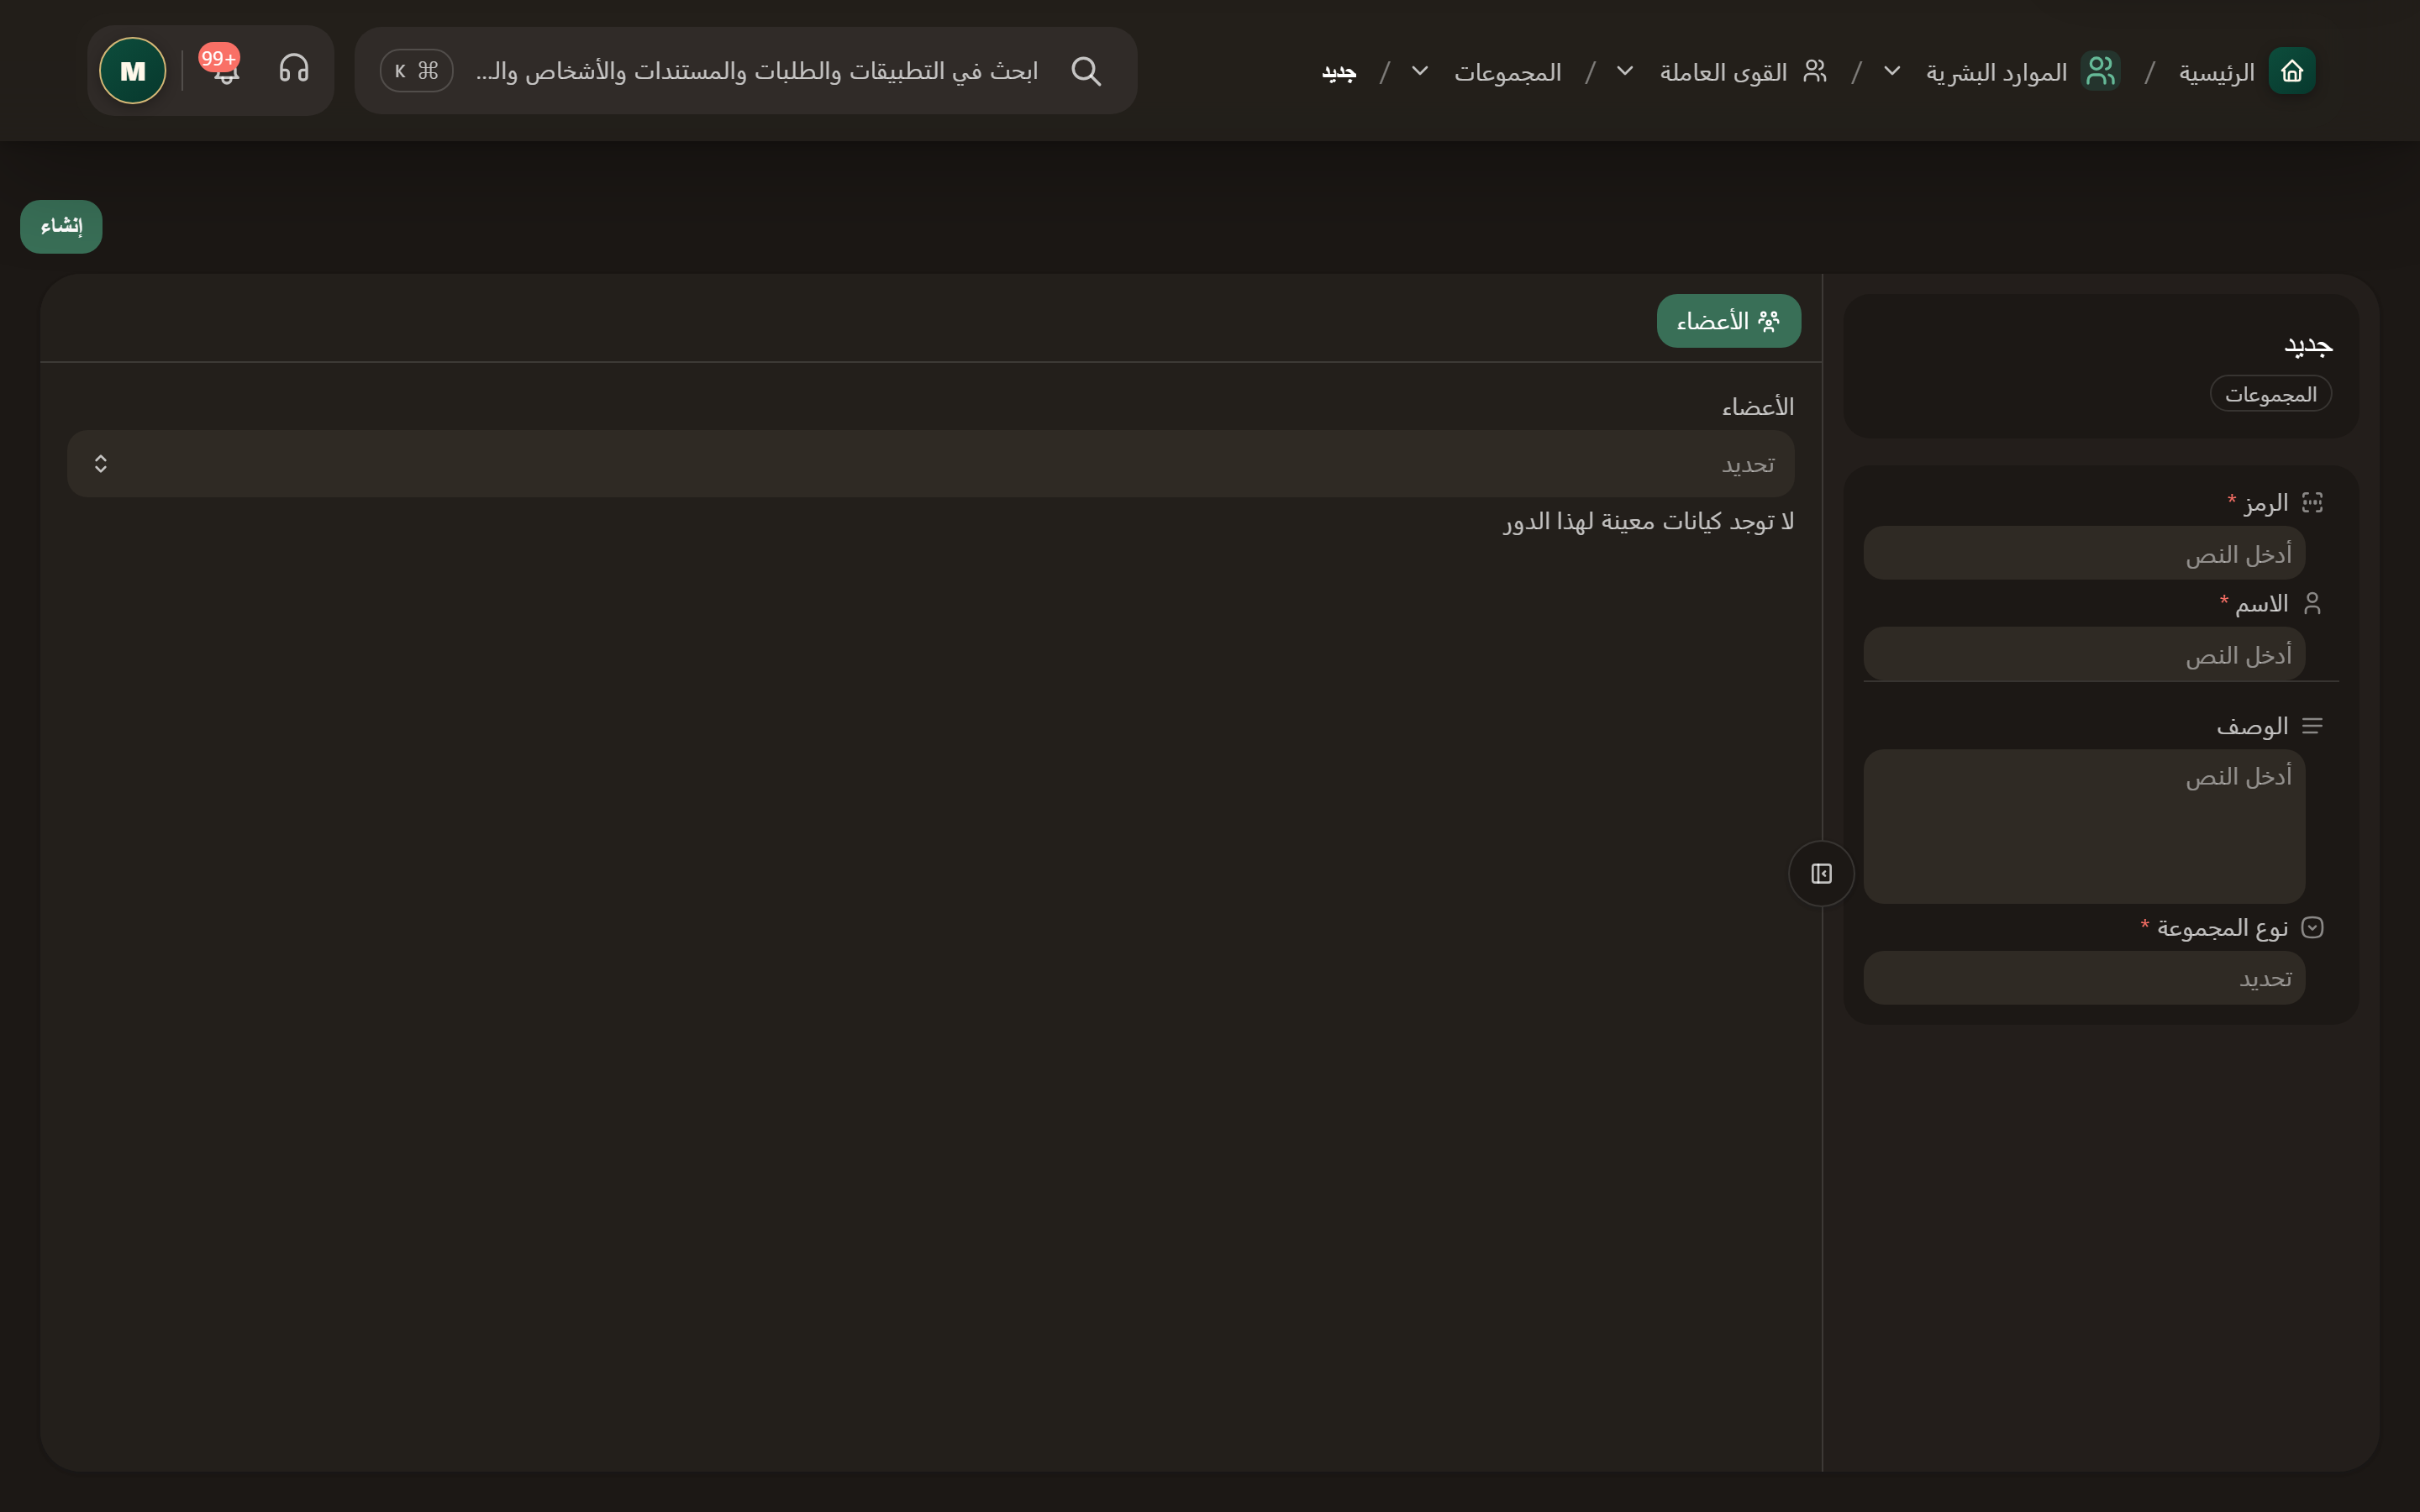
\includegraphics[width=0.95\linewidth]{figures/screens/ch03-feature-groups-tab1-ar.png}
\caption{تبويب «الأعضاء» كاملاً؛ نموذج غير محفوظ}
\label{fig:hr-groups-fulltab1}
\end{figure}

\clearpage
\section{الورديات}
\label{sec:hr-feature-shifts}

الوردية تحدد أيام العمل وساعاته واستراحاته المتوقعة. الحضور يسجل ما حدث فعلاً.

\textbf{متى تفيد؟} جدول واحد لكل من يعمل بالنمط نفسه، بدلاً من تكرار الأوقات لكل موظف. \textbf{المسار:} «الموارد البشرية» / «الوقت» / «الورديات».

\begin{figure}[H]
\centering
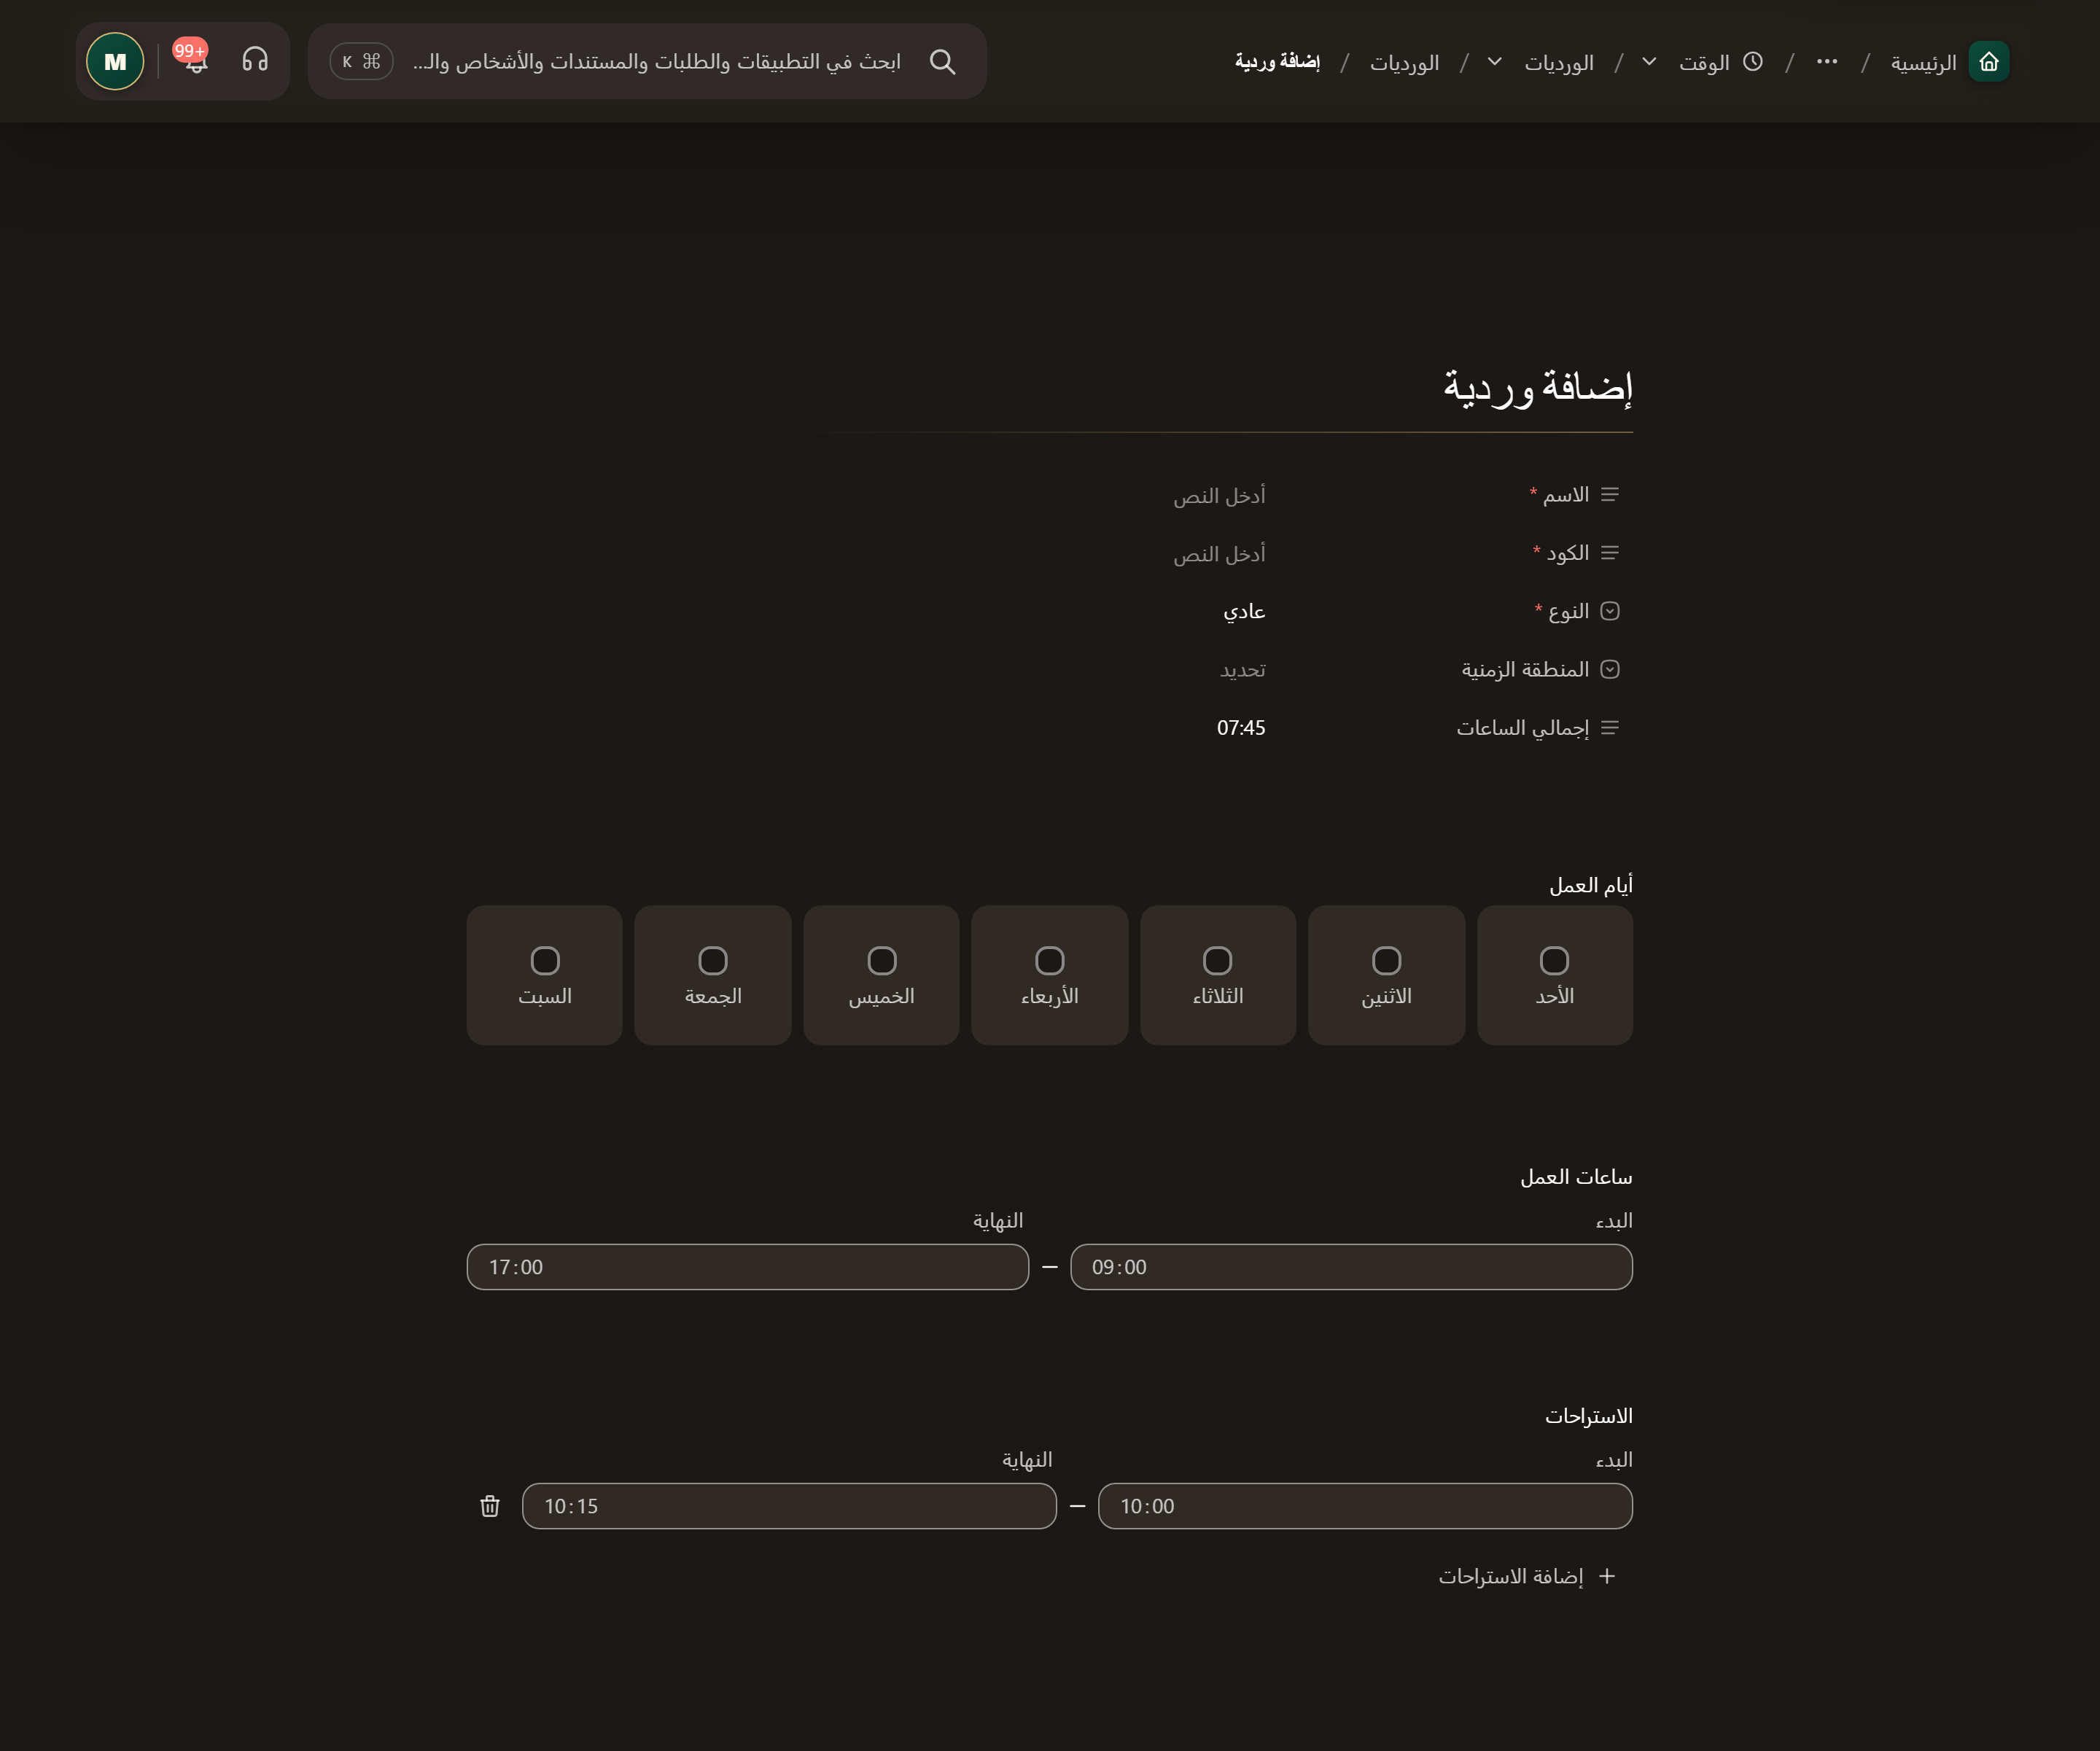
\includegraphics[width=0.95\linewidth]{figures/screens/ch03-shift-example-ar.png}
\caption{الورديات: نموذج الإضافة كاملاً؛ لم يُحفظ}
\label{fig:hr-feature-shifts-screen}
\end{figure}

\begin{table}[H]
\centering
\caption{اختيار نوع الوردية}
\label{tab:hr-shift-types}
\rcZebra
\begin{tabularx}{\linewidth}{R{2.4cm} Y Y}
\rcHeaderRow
\thh{النوع} & \thh{ماذا تُدخل؟} & \thh{مثال توضيحي}\\
عادي & فترة عمل واحدة، واستراحات عند الحاجة. & من \en{09:00} إلى \en{17:00}.\\
مقسم & أكثر من فترة عمل، دون تداخل. & من \en{09:00} إلى \en{13:00}، ثم من \en{16:00} إلى \en{20:00}.\\
مرن & مدة العمل بالساعات والدقائق. & مدة \en{08:00} دون وقت بدء أو انتهاء.\\
ماراثون & مدة العمل بالساعات والدقائق. & لا تستنتج من الاسم وحده نظام عمل وراحة معيناً.\\
\end{tabularx}
\end{table}

\begin{table}[H]
\centering
\caption{ما الذي تسجله في الوردية؟}
\label{tab:hr-feature-shifts-data}
\rcZebra
\begin{tabularx}{\linewidth}{R{3.6cm} Y}
\rcHeaderRow
\thh{الحقل} & \thh{ما الذي تضيفه؟}\\
الاسم والرمز والنوع & \req{}؛ الرمز لا يتكرر.\\
أيام العمل & \req{}: اختر يوماً واحداً على الأقل من أيام الأسبوع.\\
المنطقة الزمنية & مثل \en{Asia/Damascus} \opt{}.\\
ساعات العمل والاستراحات & للنوعين العادي والمقسم؛ وتقع الاستراحة داخل ساعات العمل \opt{}.\\
المدة & للمرن والماراثون؛ لا يمكن أن تكون \en{00:00}.\\
إجمالي الساعات & ساعات العمل بعد طرح الاستراحات \gen{}.\\
\end{tabularx}
\end{table}

\subsection{أنشئ الوردية خطوة بخطوة}
\label{sec:hr-shifts}

\begin{enumerate}
  \item افتح «الورديات» وأضف «الدوام الإداري»، الرمز \en{HZN-S-01}، النوع «عادي».
  \item اختر الأحد إلى الخميس، والمنطقة الزمنية \en{Asia/Damascus}.
  \item ساعات العمل: \en{09:00–17:00}. عدّل الاستراحة الموجودة إلى \en{13:00–13:30}؛ لا تضف استراحة ثانية.
  \item تحقق من الإجمالي \en{07:30}، ثم «حفظ». أعد فتح الوردية وتحقق من القيم.
\end{enumerate}

\begin{rcnote}[تجنب خطأ الوقت]
لا تجعل الفترات تتداخل، واجعل الاستراحة داخل ساعات العمل. \en{22:00–06:00} تنتهي في اليوم التالي. لا يُسمح بتساوي وقت البدء ووقت النهاية.
\end{rcnote}

\subsection{كيف تصل الوردية إلى الموظف؟}
\label{sec:hr-shift-inheritance}

وراثة الوردية تعني استخدام وردية المنصب أو القسم أو الموقع عندما لا تُحدد وردية خاصة للتعيين.

\begin{figure}[H]
\centering
\begin{tikzpicture}[node distance=0.4cm,stepBox/.append style={minimum width=6.5cm,text width=6.1cm,minimum height=0.7cm}]
  \node[stepBox] (a) {\RL{وردية التعيين}};
  \node[stepBox,below=of a] (p) {\RL{وردية المنصب}};
  \node[stepBox,below=of p] (n) {\RL{وردية الوحدة، ثم}\\\RL{وحداتها الأم}};
  \node[stepBox,below=of n] (l) {\RL{وردية الموقع، ثم}\\\RL{مواقعه الأم}};
  \draw[flowsTo] (a) -- (p);
  \draw[flowsTo] (p) -- (n);
  \draw[flowsTo] (n) -- (l);
\end{tikzpicture}
\rclegend
\caption{ترتيب البحث عن الوردية: ينتقل النظام إلى المستوى التالي إذا لم يجد وردية}
\label{fig:hr-shift-order}
\end{figure}

يعتمد النظام أول وردية يجدها، ولا يجمع الورديات.

\begin{enumerate}
  \item افتح «الوحدات التنظيمية» / \en{HZN-HR}. اختر «تجاوز» أولاً عند الحاجة، ثم «الدوام الإداري» في «الوردية»، واحفظ.
  \item افتح «المناصب» / مدير الموارد البشرية، وتحقق من القسم والوردية.
  \item افتح تعيين سارة وتحقق من الوردية. إن اختلفت، راجع التعيين ثم المنصب حسب المخطط.
\end{enumerate}

\textbf{تحقق:} الوردية الصحيحة تظهر في تعيين سارة. «إعادة تعيين» تعيد الوراثة. لا تُحفظ الوردية؟ راجع الاسم والرمز والأيام والفترات المتداخلة. المدة أقل من المتوقع؟ لأن الاستراحات تُطرح منها. لا تُحذف؟ لأنها مستخدمة في تعيينات أو مناصب أو سجلات حضور.

\clearpage
\section{حضوري}
\label{sec:hr-feature-my-attendance}

تعرض صفحة «حضوري» حضورك الشهري كما احتسبه النظام: أيام العمل والعطل، ولكل يوم بصماته وإجمالياته وأثره في الراتب.

\textbf{متى تفيد؟} افهم يومك قبل طلب تصحيح. اليوم الفارغ لا يثبت الغياب؛ افحص مصدر البصمات أولاً. \textbf{المسار:} «الموارد البشرية» / «الوقت» / «حضوري».

\begin{figure}[H]
\centering
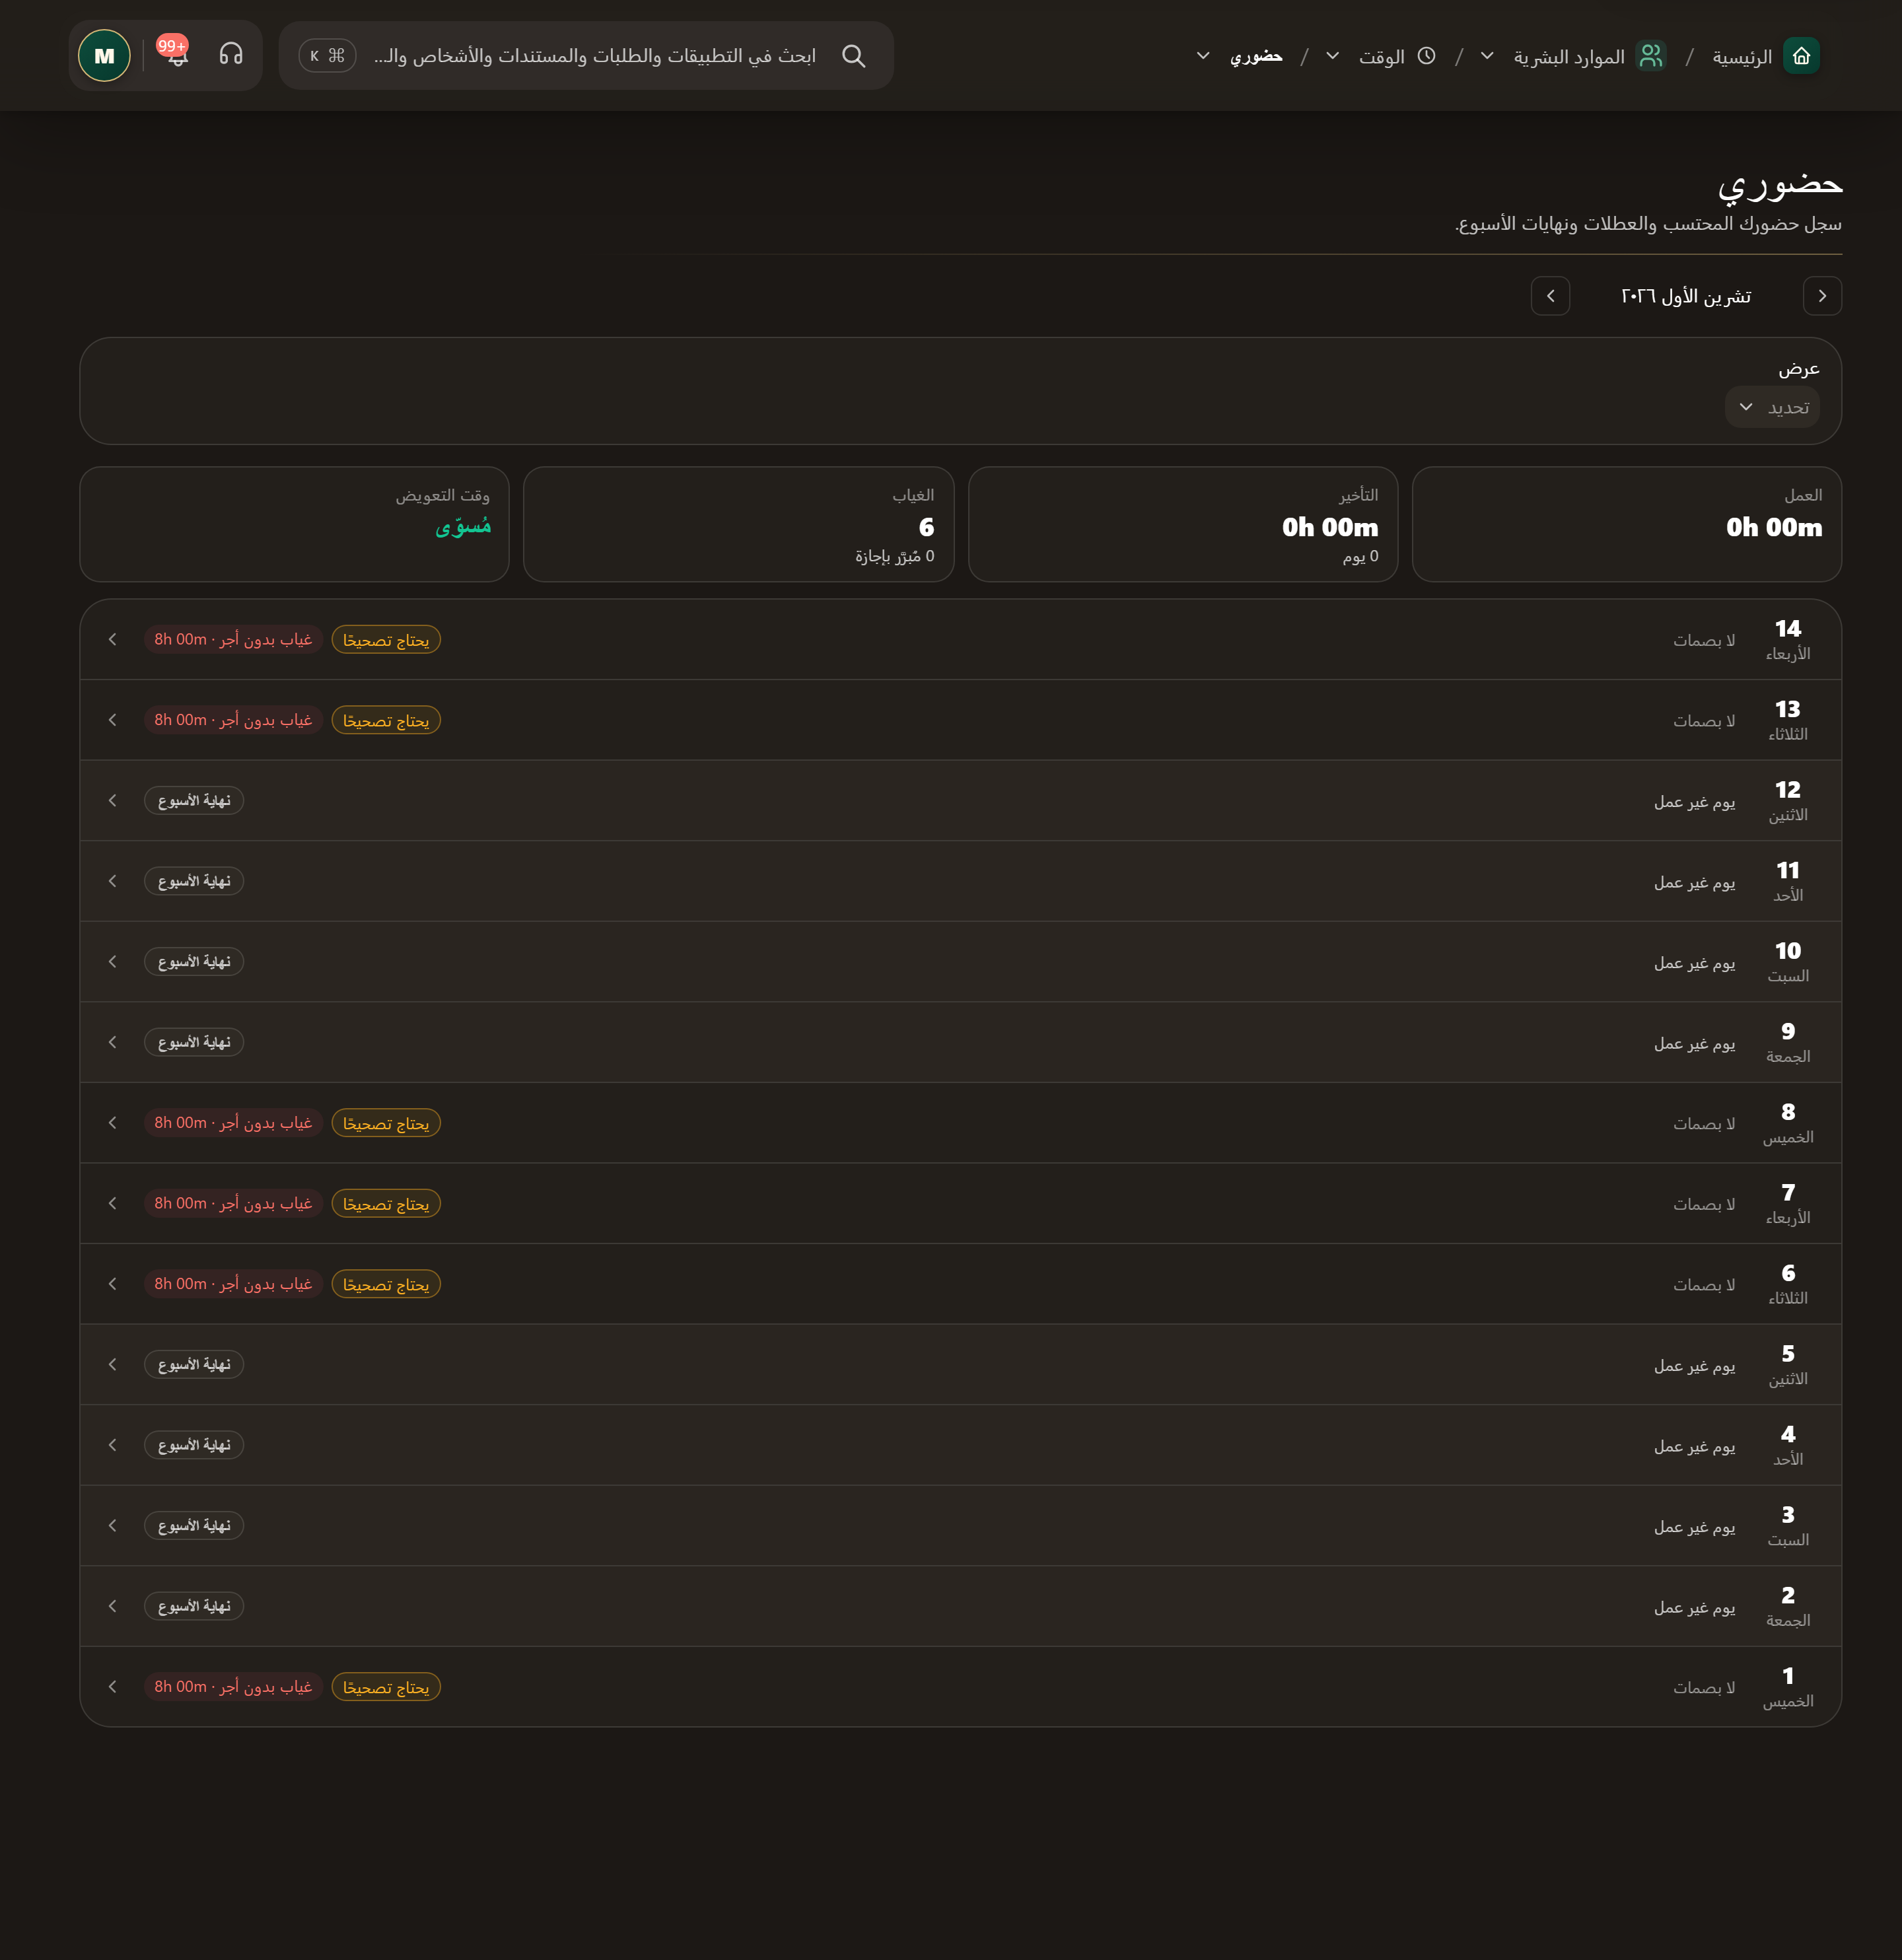
\includegraphics[width=0.95\linewidth]{figures/screens/ch03-feature-my-attendance-ar.png}
\caption{حضوري: الصفحة كاملة في بيئة الاختبار}
\label{fig:hr-feature-my-attendance-screen}
\end{figure}

\begin{table}[H]
\centering
\caption{ما الذي تراه في حضوري؟}
\label{tab:hr-feature-my-attendance-data}
\rcZebra
\begin{tabularx}{\linewidth}{R{3.6cm} Y}
\rcHeaderRow
\thh{الجزء} & \thh{ماذا يعرض؟}\\
ملخص الشهر & العمل، التأخير وعدد أيامه، الغياب وما برّرته الإجازة، وقت التعويض.\\
أيام الشهر & لكل يوم: اعتيادي، عطلة، نهاية أسبوع، لا بصمات، يحتاج تصحيحاً، مقفل.\\
صفحة اليوم & الوردية والسياسة، الخط الزمني للبصمات، «إجماليات اليوم»، «على كشف الراتب»، «كيف تم الاحتساب».\\
\end{tabularx}
\end{table}

\subsection{ما الذي يمكنك فعله؟}

\begin{itemize}
  \item التنقل بين الأشهر، ومن يوم إلى اليوم التالي.
  \item «تصحيح هذا اليوم»: أضف بصمة دخول أو خروج، واختر السبب: نسي تسجيل البصمة، عطل في الجهاز، مسح مكرر، قراءة اتجاه خاطئة، عمل خارج الموقع، أو أخرى مع تبرير.
  \item «إرسال للمراجعة»، و«سحب» الطلب ما دام قيد المراجعة.
  \item عرض حضور عضو آخر عند وجود الصلاحية؛ لكن طلب التصحيح يبقى لصاحب الحضور وحده.
\end{itemize}

\begin{figure}[H]
\centering
\begin{tikzpicture}[node distance=0.4cm,stepBox/.append style={minimum width=6cm,text width=5.6cm,minimum height=0.7cm}]
  \node[stepBox] (s0) {\RL{حضوري: اختر الشهر}\\\RL{واليوم}};
  \node[stepBox,below=of s0] (s1) {\RL{قارن الوقت المتوقع}\\\RL{بالدخول والخروج}};
  \node[stepBox,below=of s1] (s2) {\RL{راجع الإجازة والعطلة}\\\RL{إن وجدت}};
  \node[stepBox,below=of s2] (s3) {\RL{راجع التصحيح وحالة}\\\RL{القرار}};
  \draw[flowsTo] (s0) -- (s1);
  \draw[flowsTo] (s1) -- (s2);
  \draw[flowsTo] (s2) -- (s3);
\end{tikzpicture}
\rclegend
\caption{راجع يوماً واحداً}
\label{fig:hr-day-review}
\end{figure}

\subsection{جرّب وراجع}

\begin{enumerate}
  \item افتح «حضوري»، واختر الشهر ثم اليوم.
  \item قارن الوردية بالدخول والخروج والمدة، واقرأ «كيف تم الاحتساب».
  \item إن نقصت بصمة، اختر «تصحيح هذا اليوم»، وأضفها مع السبب، ثم «إرسال للمراجعة».
\end{enumerate}

\textbf{تحقق:} يظهر على اليوم أن التصحيح قيد المراجعة. الوردية تحدد الوقت المتوقع، والسياسة تحدد التأخر والعمل الإضافي؛ لا تفترض خصماً تلقائياً. إن غاب زر التصحيح، فربما انتهت مهلة التصحيح.

\clearpage
\section{جداول الدوام}
\label{sec:hr-feature-timesheets}

جداول الدوام تعرض حضور الفريق ليوم أو أسبوع أو شهر، وتتيح اعتماد الوقت المسجل.

\textbf{متى تفيد؟} مراجعة أسبوع الفريق، أو تجهيز الوقت قبل احتساب الرواتب. \textbf{المسار:} «الموارد البشرية» / «الوقت» / «جداول الدوام».

\begin{figure}[H]
\centering
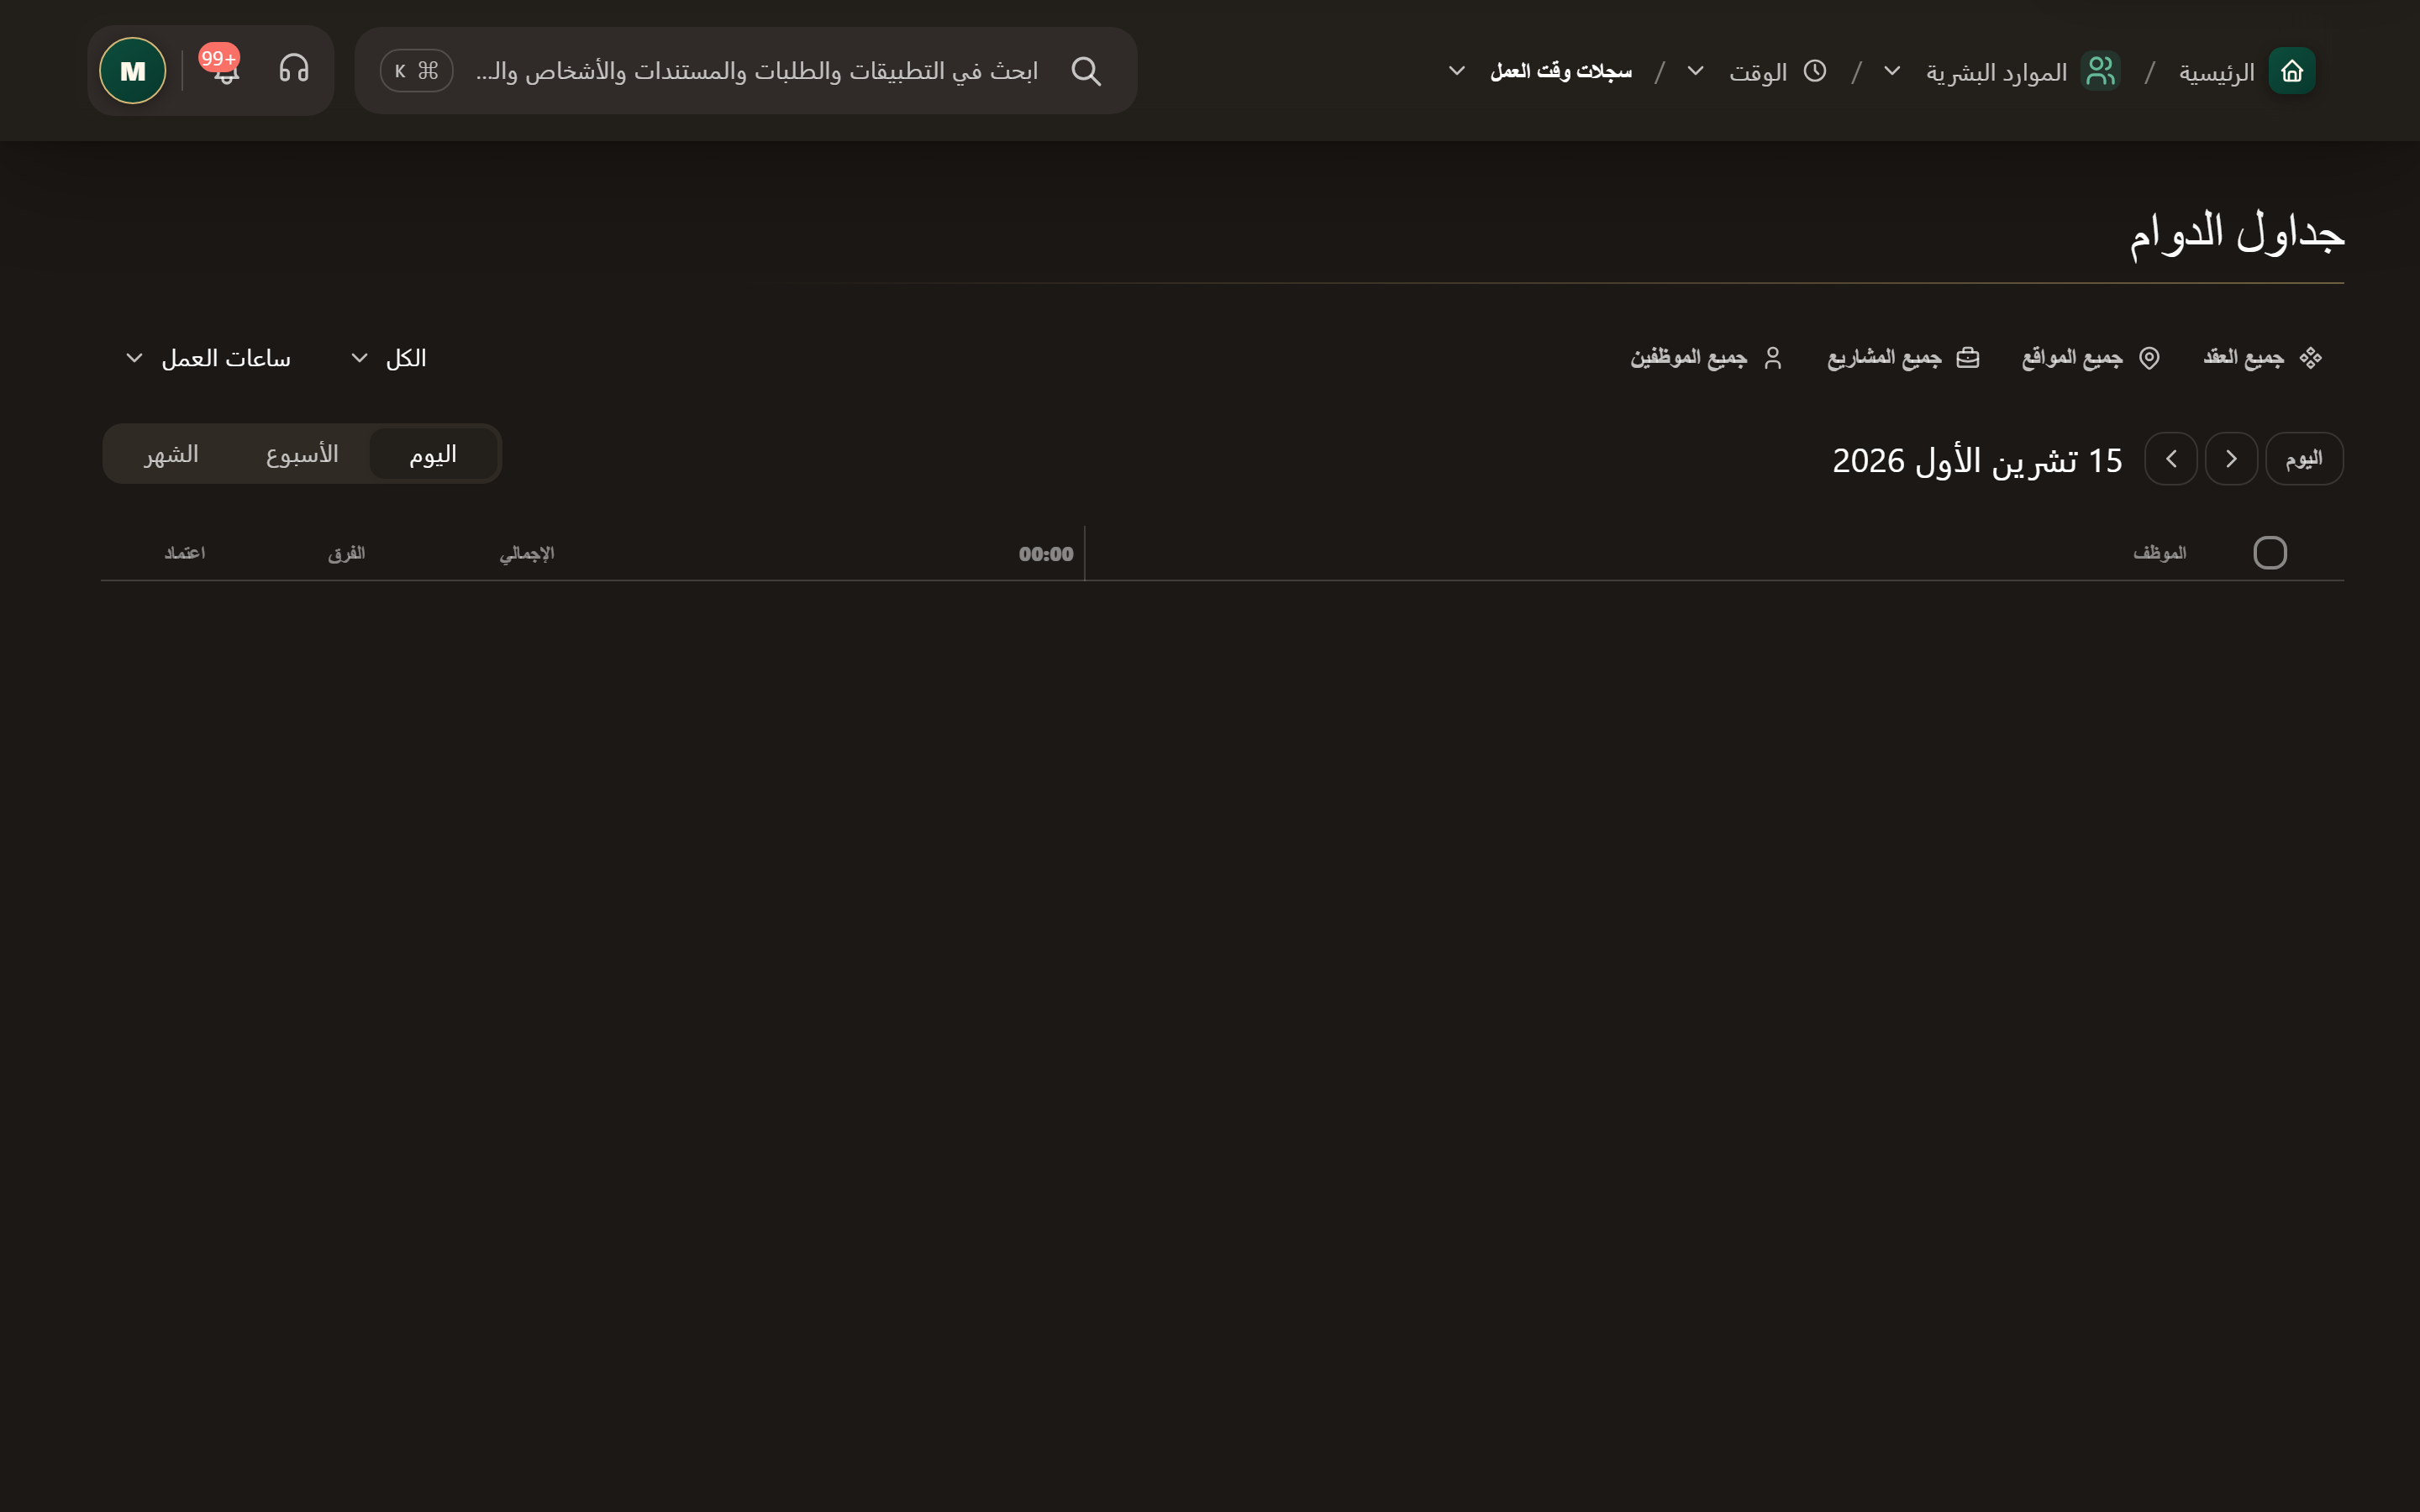
\includegraphics[width=0.95\linewidth]{figures/screens/ch03-feature-timesheets-ar.png}
\caption{جداول الدوام: الصفحة كاملة في بيئة الاختبار}
\label{fig:hr-feature-timesheets-screen}
\end{figure}

\begin{table}[H]
\centering
\caption{ما الذي تراه في جداول الدوام؟}
\label{tab:hr-feature-timesheets-data}
\rcZebra
\begin{tabularx}{\linewidth}{R{3.6cm} Y}
\rcHeaderRow
\thh{الجزء} & \thh{ماذا يعرض؟}\\
التصفية & الوحدات والمواقع والمشاريع والموظفون، والساعات: العمل فقط، أو مع الإجازات المبررة، أو مع المدفوعة.\\
الفترة & «اليوم»، أو يوم أو أسبوع أو شهر.\\
خلية اليوم & الدخول والاستراحة والخروج وإجمالي العمل؛ أو اسم العطلة.\\
الإجماليات & متوسط وقت العمل، متوسط التأخير، الإجمالي، «الفرق» عن المتوقع.\\
\end{tabularx}
\end{table}

\subsection{ما الذي يمكنك فعله؟}

\begin{itemize}
  \item عرض اليوم: خط زمني لكل موظف بالعمل والاستراحة والغياب غير المبرر.
  \item «اعتماد» صف، أو حدد عدة صفوف واعتمدها معاً؛ واعرض «الموافق فقط» أو «غير الموافق فقط».
  \item النقر على علامة الاختلاف يفتح تصحيحات الحضور. لا يمكن الإضافة أو الاستيراد هنا.
\end{itemize}

\begin{figure}[H]
\centering
\begin{tikzpicture}[node distance=0.5cm,stepBox/.append style={minimum width=6.5cm,text width=6.1cm,minimum height=0.8cm}]
  \node[stepBox] (a) {\RL{اختيار الأشخاص}\\\RL{والفترة}};
  \node[stepBox,below=of a] (b) {\RL{مراجعة الأيام}\\\RL{والإجماليات}};
  \node[stepBox,below=of b] (c) {\RL{فحص الاختلافات}};
  \draw[flowsTo] (a) -- (b);
  \draw[flowsTo] (b) -- (c);
\end{tikzpicture}
\rclegend
\caption{خطوات الاستخدام؛ الأسهم لا تعني معالجة تلقائية}
\label{fig:hr-feature-timesheets-flow}
\end{figure}

\subsection{جرّب وراجع}

\begin{enumerate}
  \item افتح «جداول الدوام»، واختر قسم الموارد البشرية و«أسبوع».
  \item اقرأ أيام كل موظف والإجماليات. إن ظهرت قيمة غير متوقعة، افتح اليوم ووردية الموظف.
  \item في عرض اليوم، اعتمد الصفوف الصحيحة.
\end{enumerate}

\textbf{تحقق:} تتغير حالة الصفوف المعتمدة. تحقق من الأشخاص والتواريخ قبل اعتبار الجدول الفارغ نقصاً في الحضور.

\clearpage
\section{أنواع الإجازات}
\label{sec:hr-feature-leave-types}

يحدد نوع الإجازة قواعدها: هل هي مدفوعة، وكيف تؤثر في الحضور، وكيف يُخصص رصيدها. مثال: «سنوية مدفوعة».

\textbf{متى تفيد؟} عرّف القاعدة مرة واحدة لتُسجَّل كل الإجازات بتصنيف موحد. النوع ليس إجازة لموظف في تاريخ محدد. \textbf{المسار:} «الموارد البشرية» / «الوقت» / «أنواع الإجازات».

\begin{figure}[H]
\centering
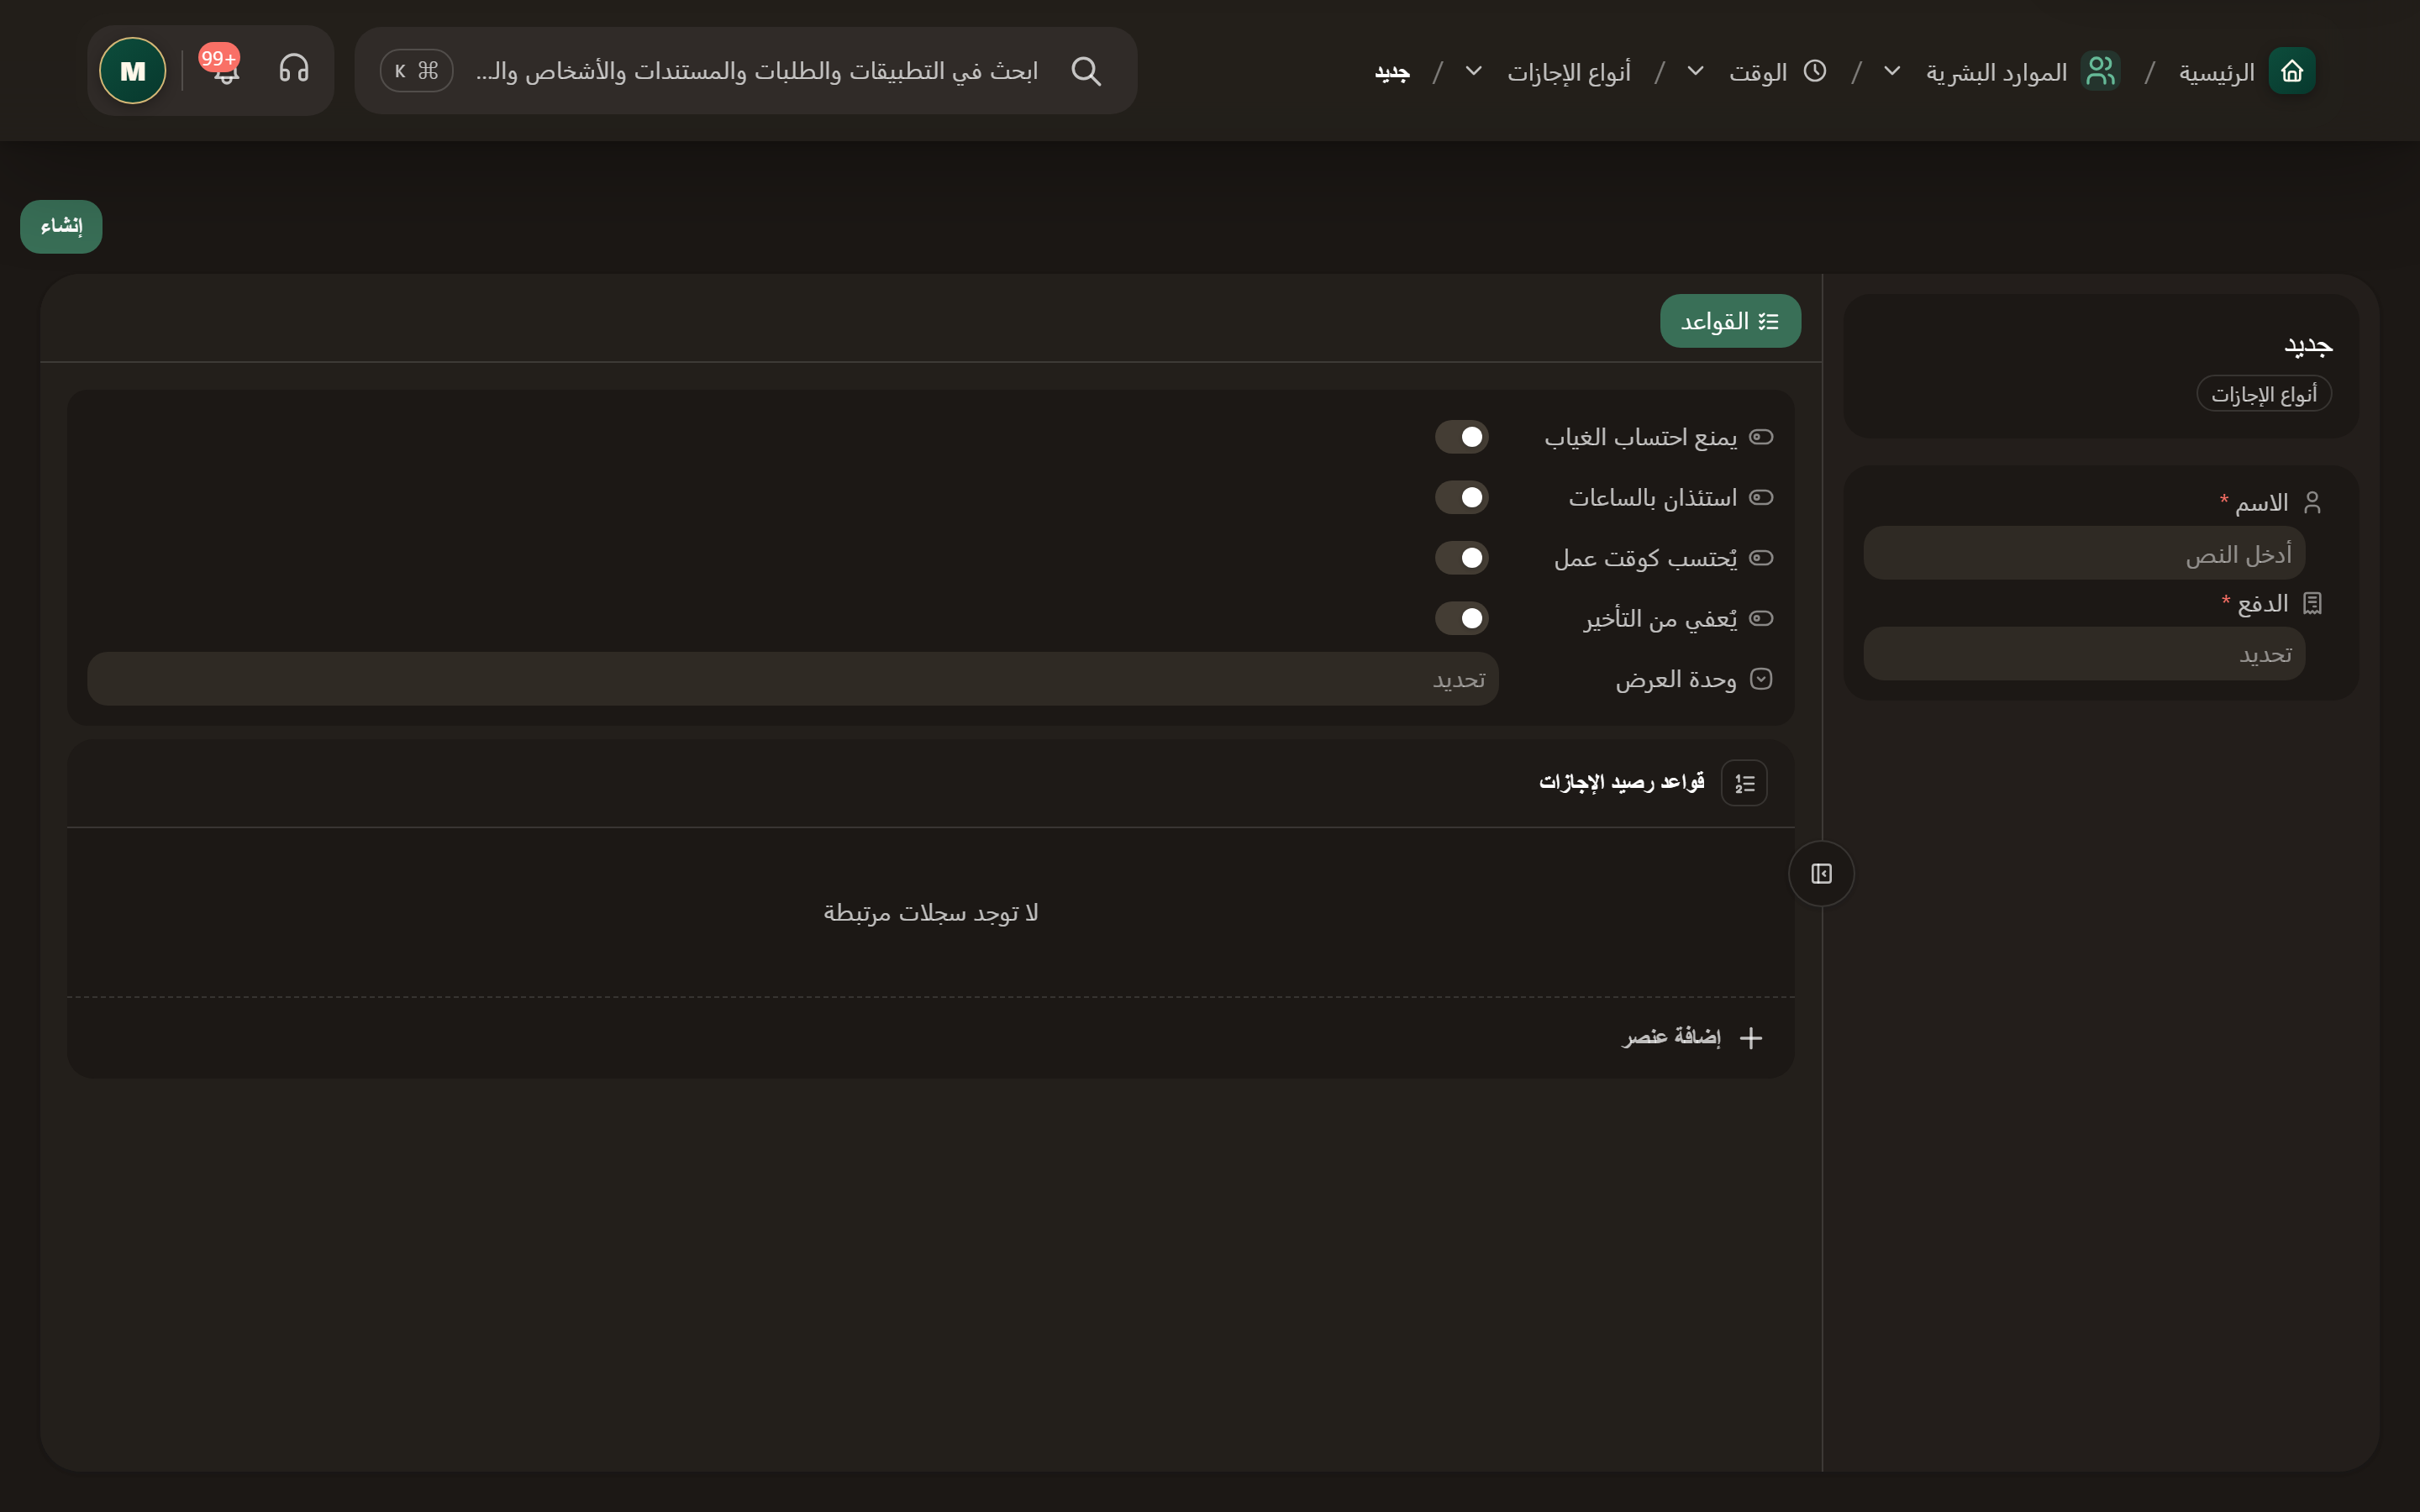
\includegraphics[width=0.95\linewidth]{figures/screens/ch03-leave-type-fields-ar.png}
\caption{أنواع الإجازات: الدفع والقواعد؛ لم يُحفظ}
\label{fig:hr-feature-leave-types-screen}
\end{figure}

\begin{table}[H]
\centering
\caption{ما الذي تسجله في نوع الإجازة؟}
\label{tab:hr-feature-leave-types-data}
\rcZebra
\begin{tabularx}{\linewidth}{R{3.6cm} Y}
\rcHeaderRow
\thh{التبويب أو الحقل} & \thh{ما الذي تضيفه؟}\\
الاسم & \req{}؛ مثل سنوية مدفوعة، مرضية، استئذان.\\
الدفع & \req{}: مدفوع، غير مدفوع، أو مدفوع جزئياً مع نسبة الدفع.\\
القواعد & يمنع احتساب الغياب، استئذان بالساعات، يُحتسب كوقت عمل، يُعفي من التأخير، وحدة العرض.\\
قواعد رصيد الإجازات & لمن يُخصص، أيام أو ساعات وكميتها، التكرار: أسبوعي أو شهري أو سنوي أو مرة واحدة، الانتهاء، تاريخ التأثير، الحالة.\\
\end{tabularx}
\end{table}

يُمنح الرصيد بقاعدة الرصيد لمن خُصصت له فقط؛ فوجود النوع لا يمنح الجميع رصيداً. لا يُحذف نوع مستخدم في إجازات.

\begin{figure}[H]
\centering
\begin{tikzpicture}[node distance=0.5cm,stepBox/.append style={minimum width=6.5cm,text width=6.1cm,minimum height=0.8cm}]
  \node[stepBox] (a) {\RL{تعريف نوع الإجازة}};
  \node[stepBox,below=of a] (b) {\RL{قاعدة الرصيد}\\\RL{والمشمولون بها}};
  \node[stepBox,below=of b] (c) {\RL{تسجيل إجازة مؤرخة}};
  \draw[flowsTo] (a) -- (b);
  \draw[flowsTo] (b) -- (c);
\end{tikzpicture}
\rclegend
\caption{خطوات الاستخدام؛ الأسهم لا تعني معالجة تلقائية}
\label{fig:hr-feature-leave-types-flow}
\end{figure}

\subsection{جرّب وراجع}

\begin{enumerate}
  \item افتح «أنواع الإجازات» وابحث عن النوع قبل إضافته.
  \item إن كنت مخوّلاً، أضف «سنوية مدفوعة» واختر «مدفوع»، ثم احفظ.
  \item في تبويب «القواعد» أضف قاعدة رصيد: المخصص لهم، «الأيام»، الكمية، «سنوي»، الانتهاء، تاريخ التأثير، «نشط». احفظ.
\end{enumerate}

\textbf{تحقق:} أعد الفتح وراجع الدفع والقاعدة. يظهر الرصيد في ملف العضو، تبويب الحضور.

\begin{figure}[H]
\centering
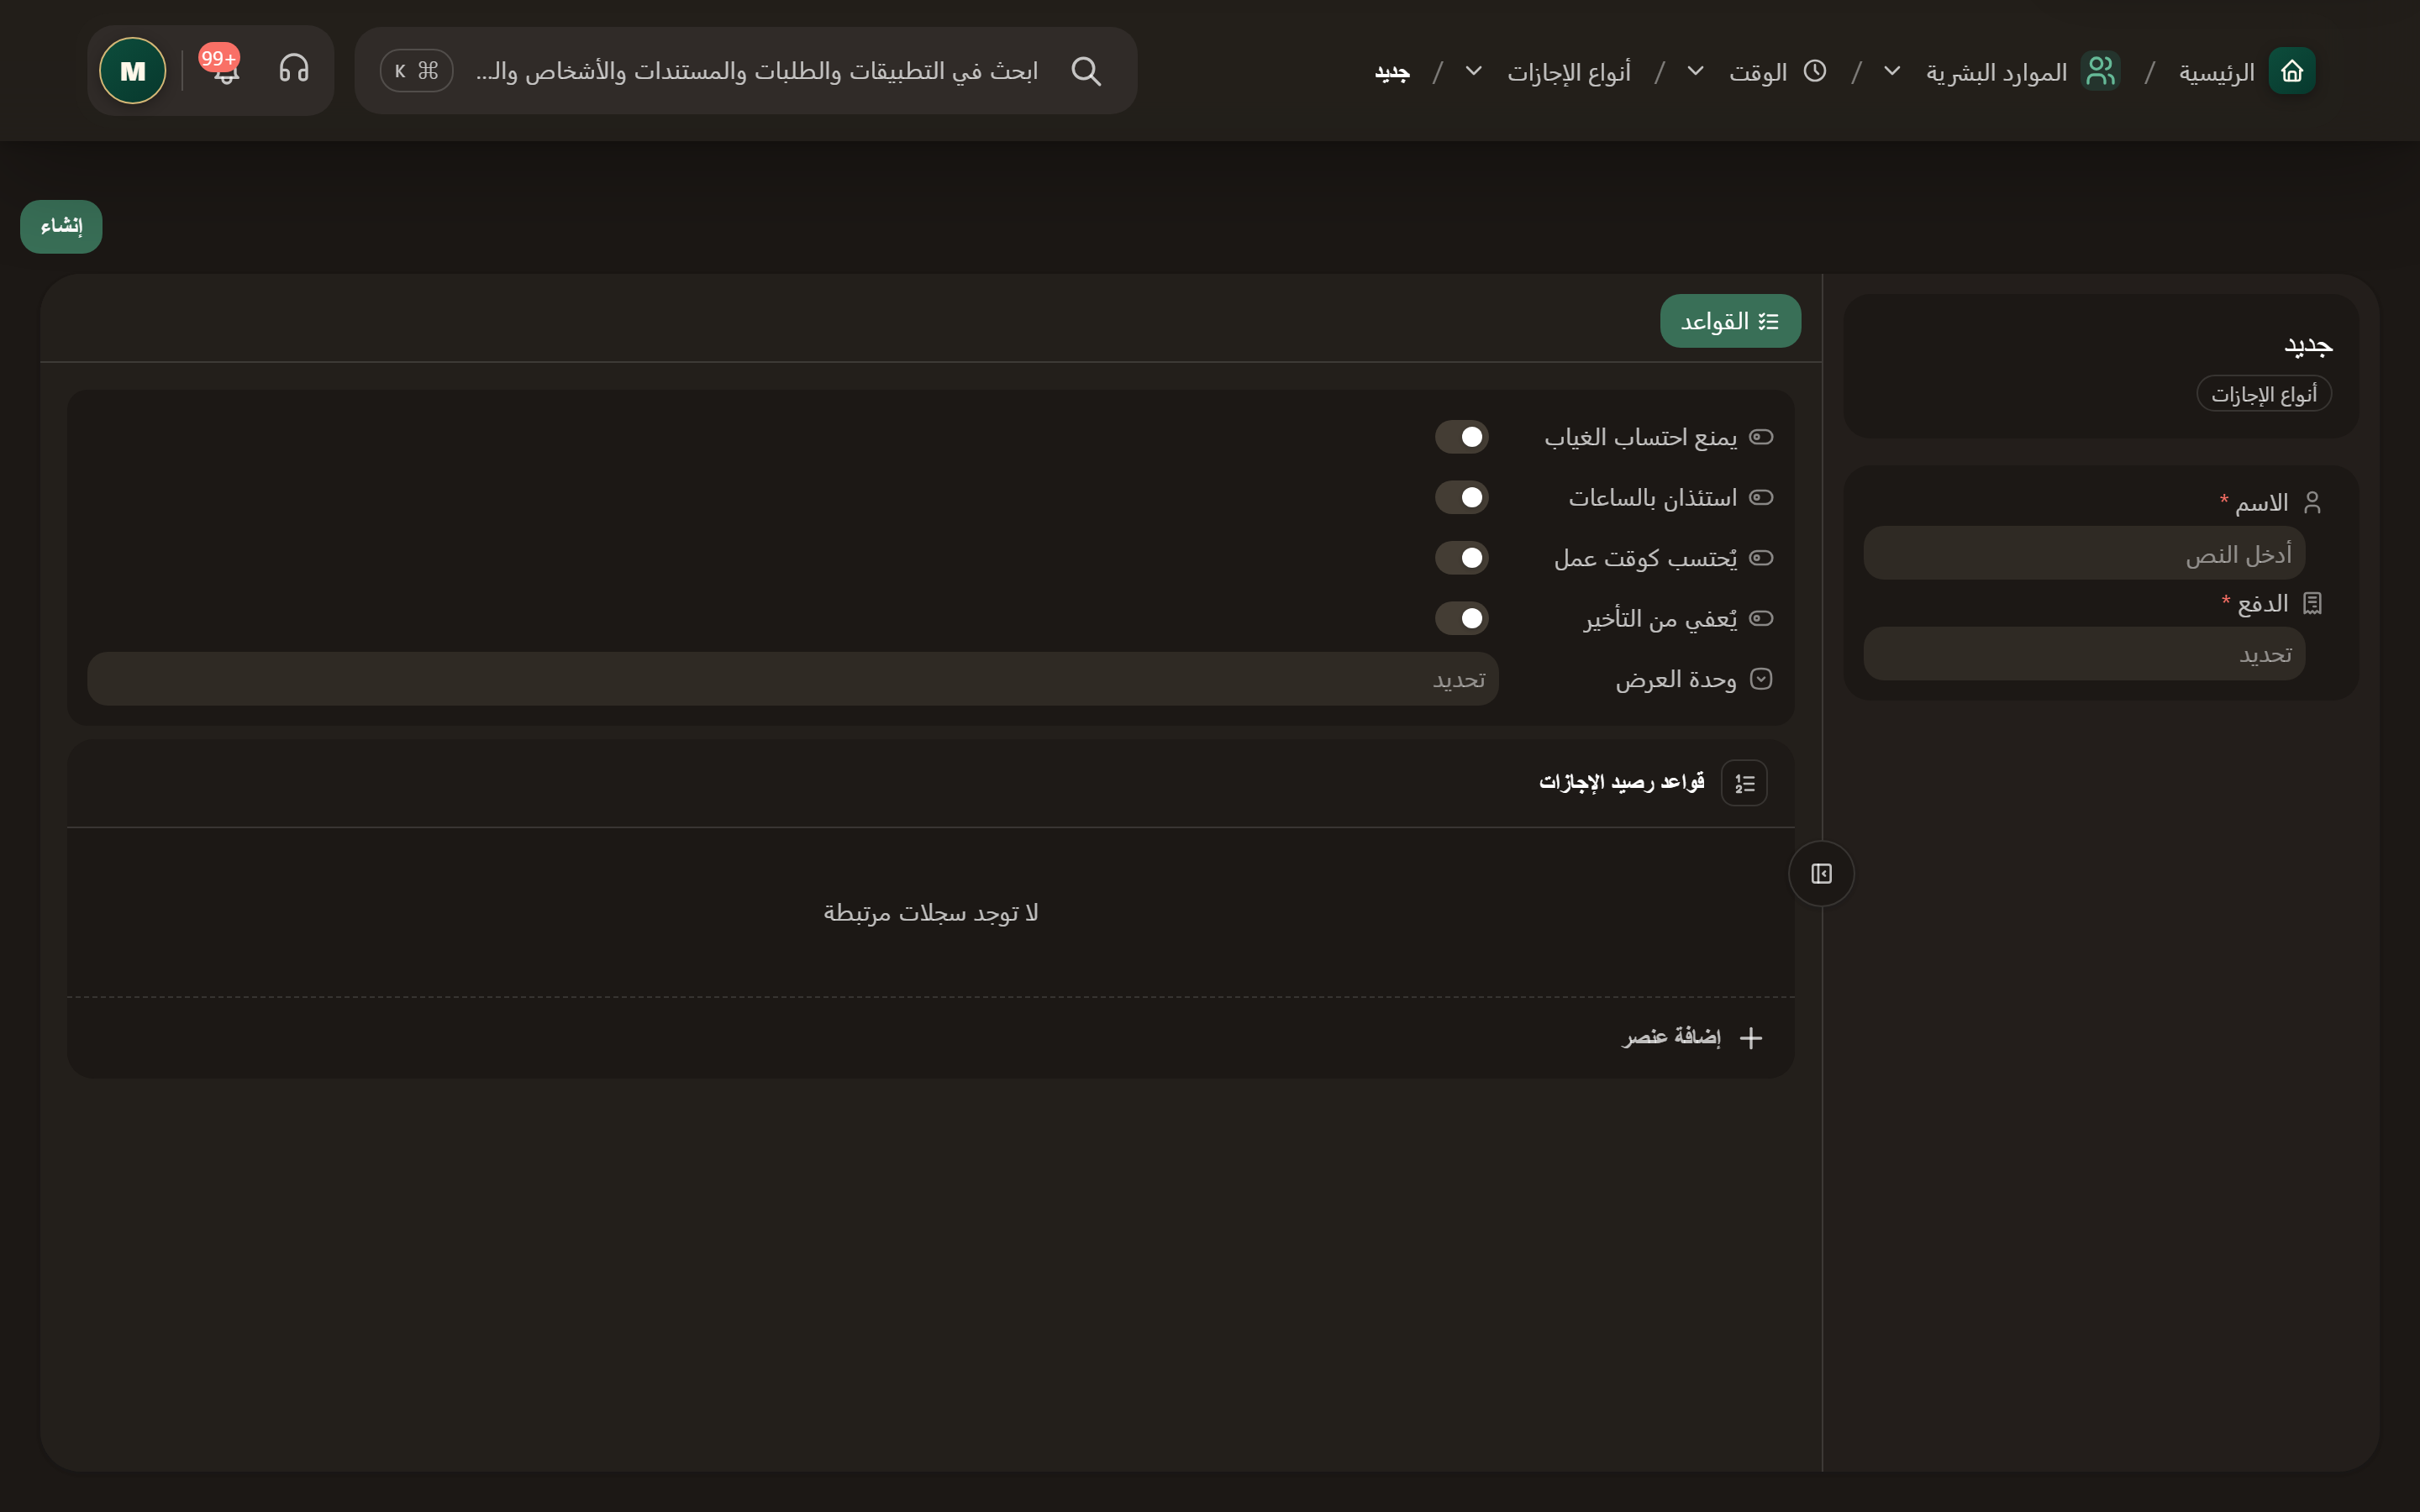
\includegraphics[width=0.95\linewidth]{figures/screens/ch03-leave-type-fields-tab1-ar.png}
\caption{تبويب «القواعد» كاملاً؛ نموذج غير محفوظ}
\label{fig:hr-leave-types-fulltab1}
\end{figure}

\clearpage
\section{الإجازات}
\label{sec:hr-feature-leaves}

يربط سجل الإجازة الموظف بنوع الإجازة، ويحدد تاريخ ووقت بدايتها ونهايتها. وله حالة: قيد الانتظار، معتمدة، أو مرفوضة.

\textbf{متى تفيد؟} تسجيل غياب سارة المعتمد ليظهر في حضورها وراتبها. العطلة مشتركة للفريق؛ الإجازة تخص موظفاً. \textbf{المسار:} «الموارد البشرية» / «الوقت» / «الإجازات».

\begin{figure}[H]
\centering
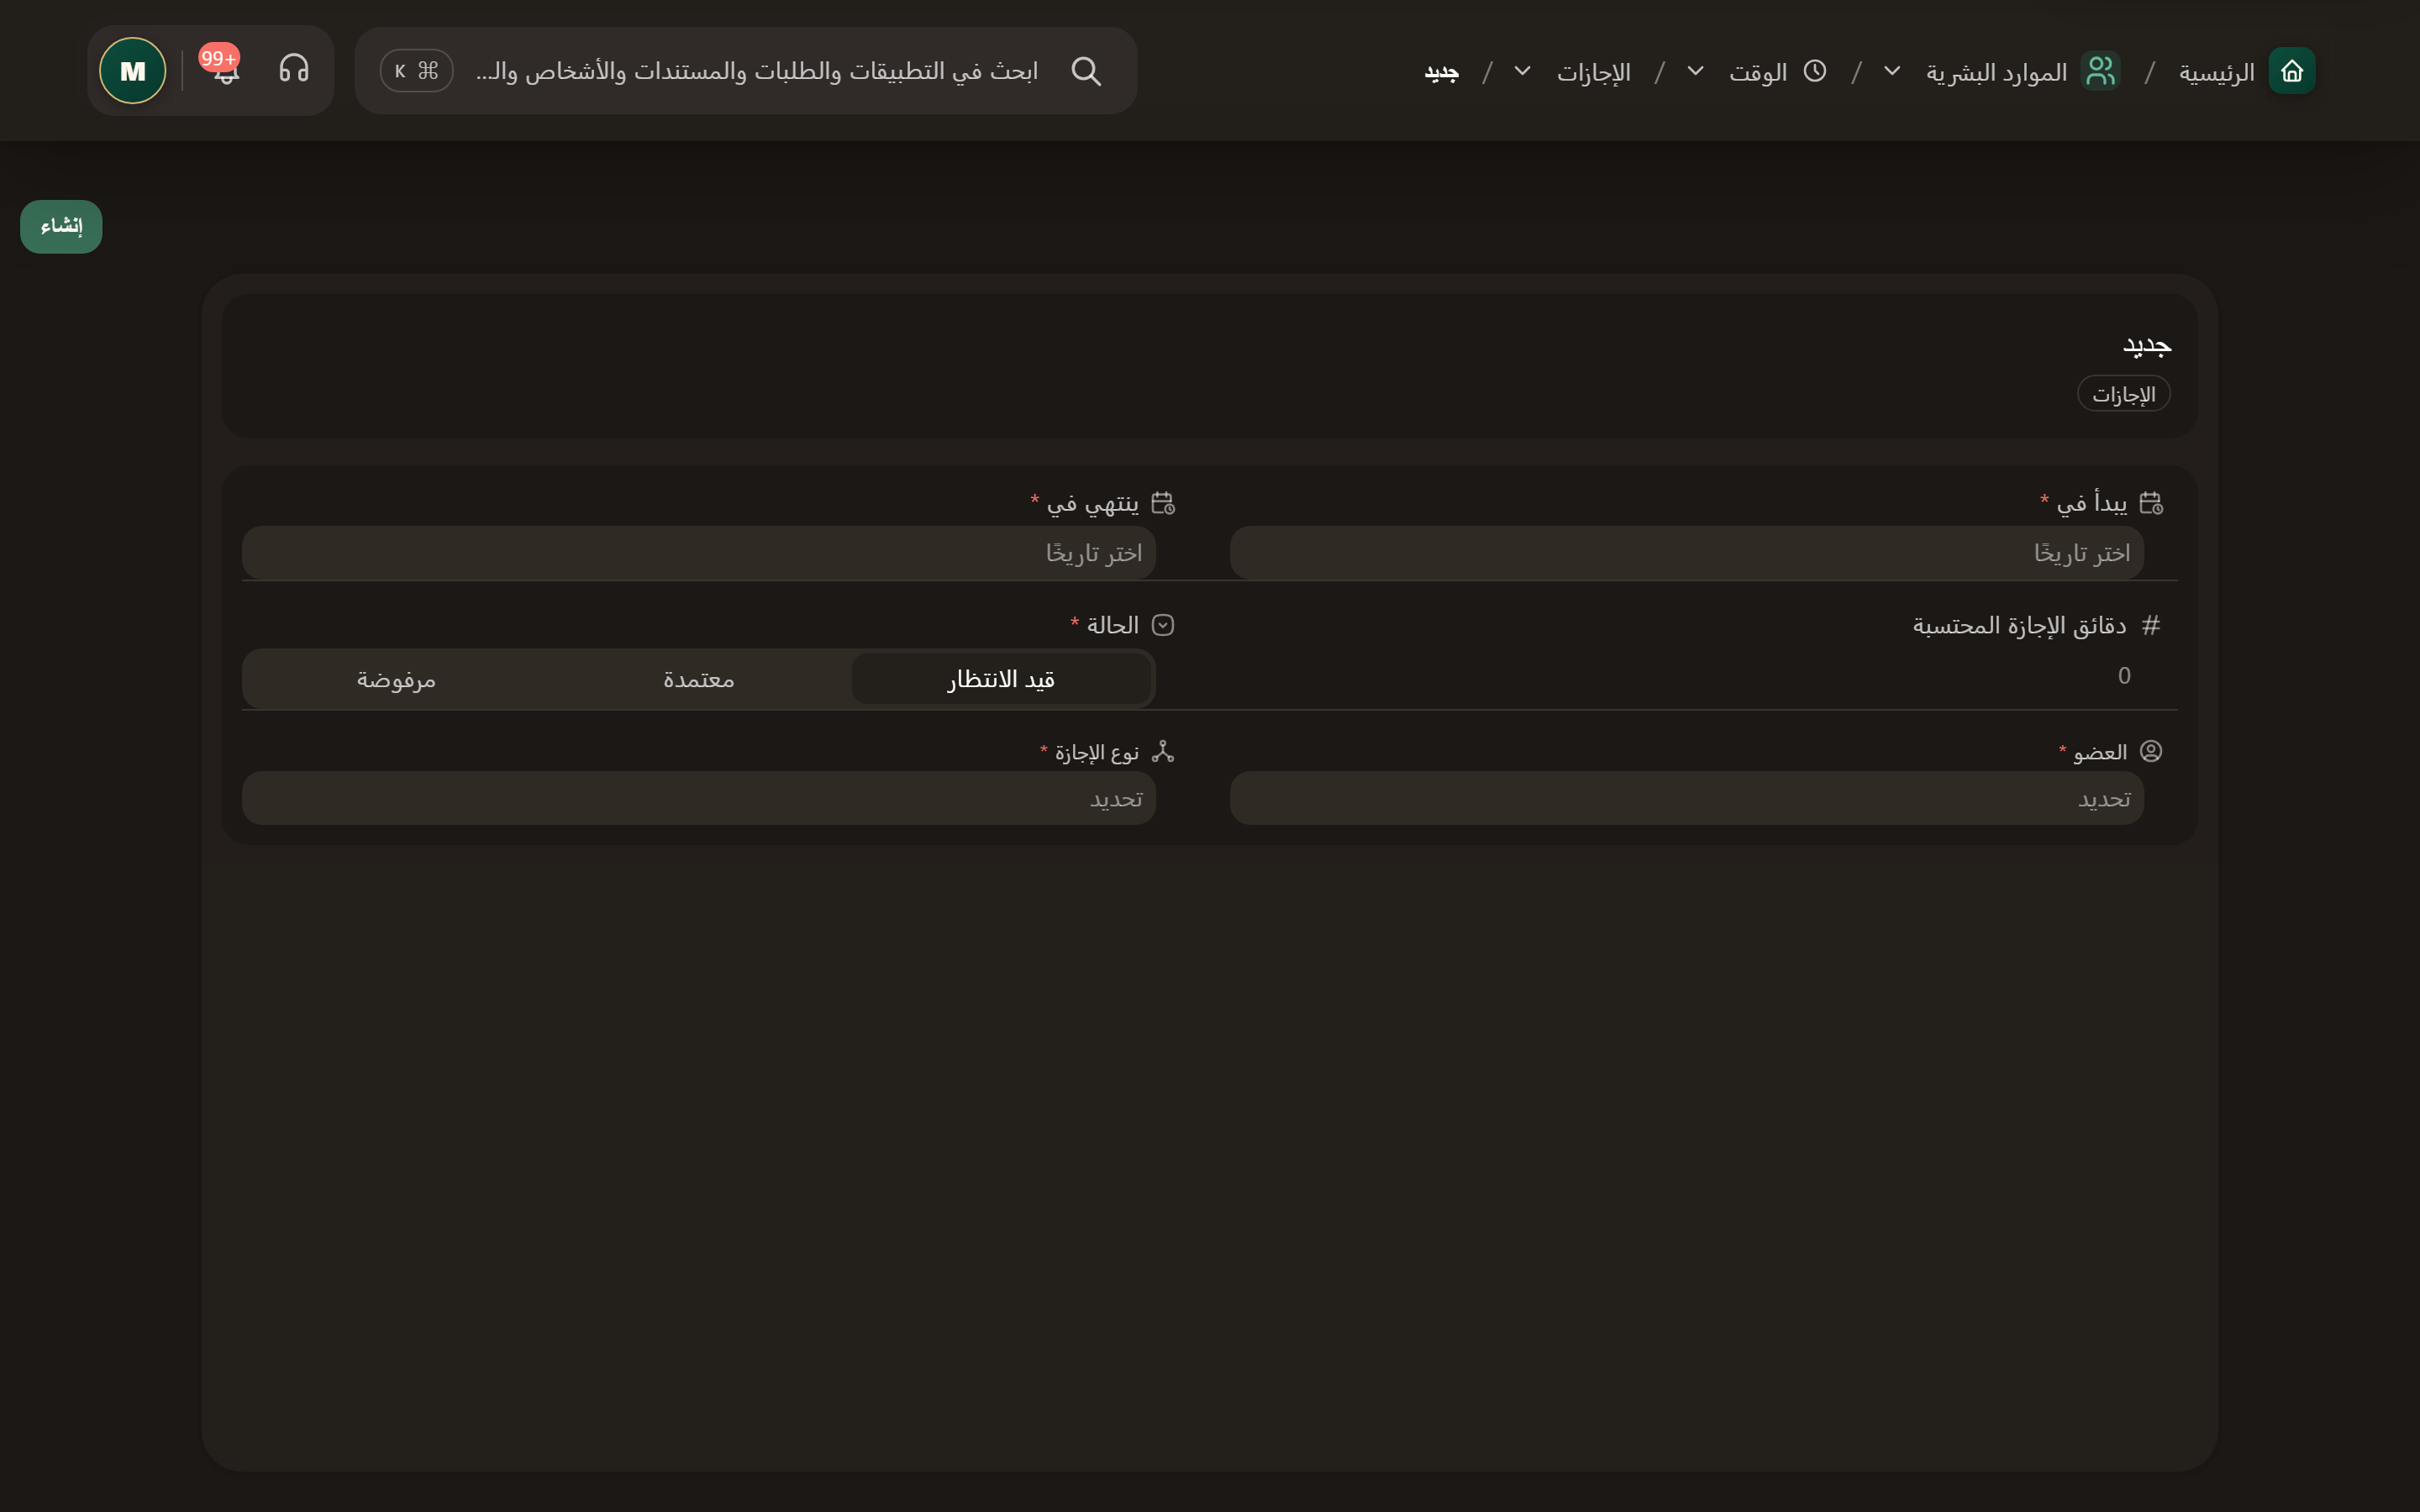
\includegraphics[width=0.95\linewidth]{figures/screens/ch03-leave-fields-ar.png}
\caption{الإجازات: الموظف والفترة والحالة؛ لم يُحفظ}
\label{fig:hr-feature-leaves-screen}
\end{figure}

\begin{table}[H]
\centering
\caption{ما الذي تسجله في الإجازة؟}
\label{tab:hr-feature-leaves-data}
\rcZebra
\begin{tabularx}{\linewidth}{R{3.6cm} Y}
\rcHeaderRow
\thh{الحقل} & \thh{ما الذي تضيفه؟}\\
العضو ونوع الإجازة & \req{}.\\
يبدأ في وينتهي في & \req{}: تاريخ ووقت.\\
الحالة & \req{}: قيد الانتظار افتراضياً، ثم معتمدة أو مرفوضة.\\
دقائق الإجازة المحتسبة & مدة الإجازة الفعلية \gen{}.\\
\end{tabularx}
\end{table}

تظهر الإجازة أيضاً في ملف العضو، تبويب الحضور. لا يوجد زر اعتماد منفصل؛ تختار الحالة في السجل نفسه بعد الموافقة.

\begin{figure}[H]
\centering
\begin{tikzpicture}[node distance=0.4cm,stepBox/.append style={minimum width=6cm,text width=5.6cm,minimum height=0.7cm}]
  \node[stepBox] (s0) {\RL{راجع النوع وطريقة}\\\RL{الدفع}};
  \node[stepBox,below=of s0] (s1) {\RL{احصل على الموافقة}};
  \node[stepBox,below=of s1] (s2) {\RL{سجّل الموظف والتاريخ}\\\RL{والمدة}};
  \node[stepBox,below=of s2] (s3) {\RL{احفظ وراجع اليوم}\\\RL{والراتب}};
  \draw[flowsTo] (s0) -- (s1);
  \draw[flowsTo] (s1) -- (s2);
  \draw[flowsTo] (s2) -- (s3);
\end{tikzpicture}
\rclegend
\caption{من نوع الإجازة إلى مراجعة يوم الموظف}
\label{fig:hr-leave-flow}
\end{figure}

\subsection{جرّب وراجع}

\begin{enumerate}
  \item تأكد من الموافقة والتواريخ ورصيد سارة. افتح «الإجازات» وابحث عن سجل سابق.
  \item أضف: سارة، «سنوية مدفوعة»، تاريخ ووقت البدء والانتهاء، والحالة «معتمدة». احفظ.
  \item أعد فتح السجل وراجع المدة المحتسبة، ثم افتح اليوم في حضوري.
\end{enumerate}

\textbf{تحقق:} يظهر اليوم في حضوري مبرراً بإجازة. إن غاب الأثر، راجع التاريخ والنوع والحالة؛ «قيد الانتظار» لا تبرر الغياب.

\clearpage
\section{مجموعات العطل الرسمية}
\label{sec:hr-feature-holiday-groups}

مجموعة العطل تقويم مشترك للعطل الرسمية، ويتبعه من تُسند إليهم المجموعة.

\textbf{متى تفيد؟} يتبع الفريق تقويم عطل واحداً، دون تسجيل كل عطلة إجازةً لكل موظف. \textbf{المسار:} «الموارد البشرية» / «الوقت» / «مجموعات العطل الرسمية».

\begin{figure}[H]
\centering
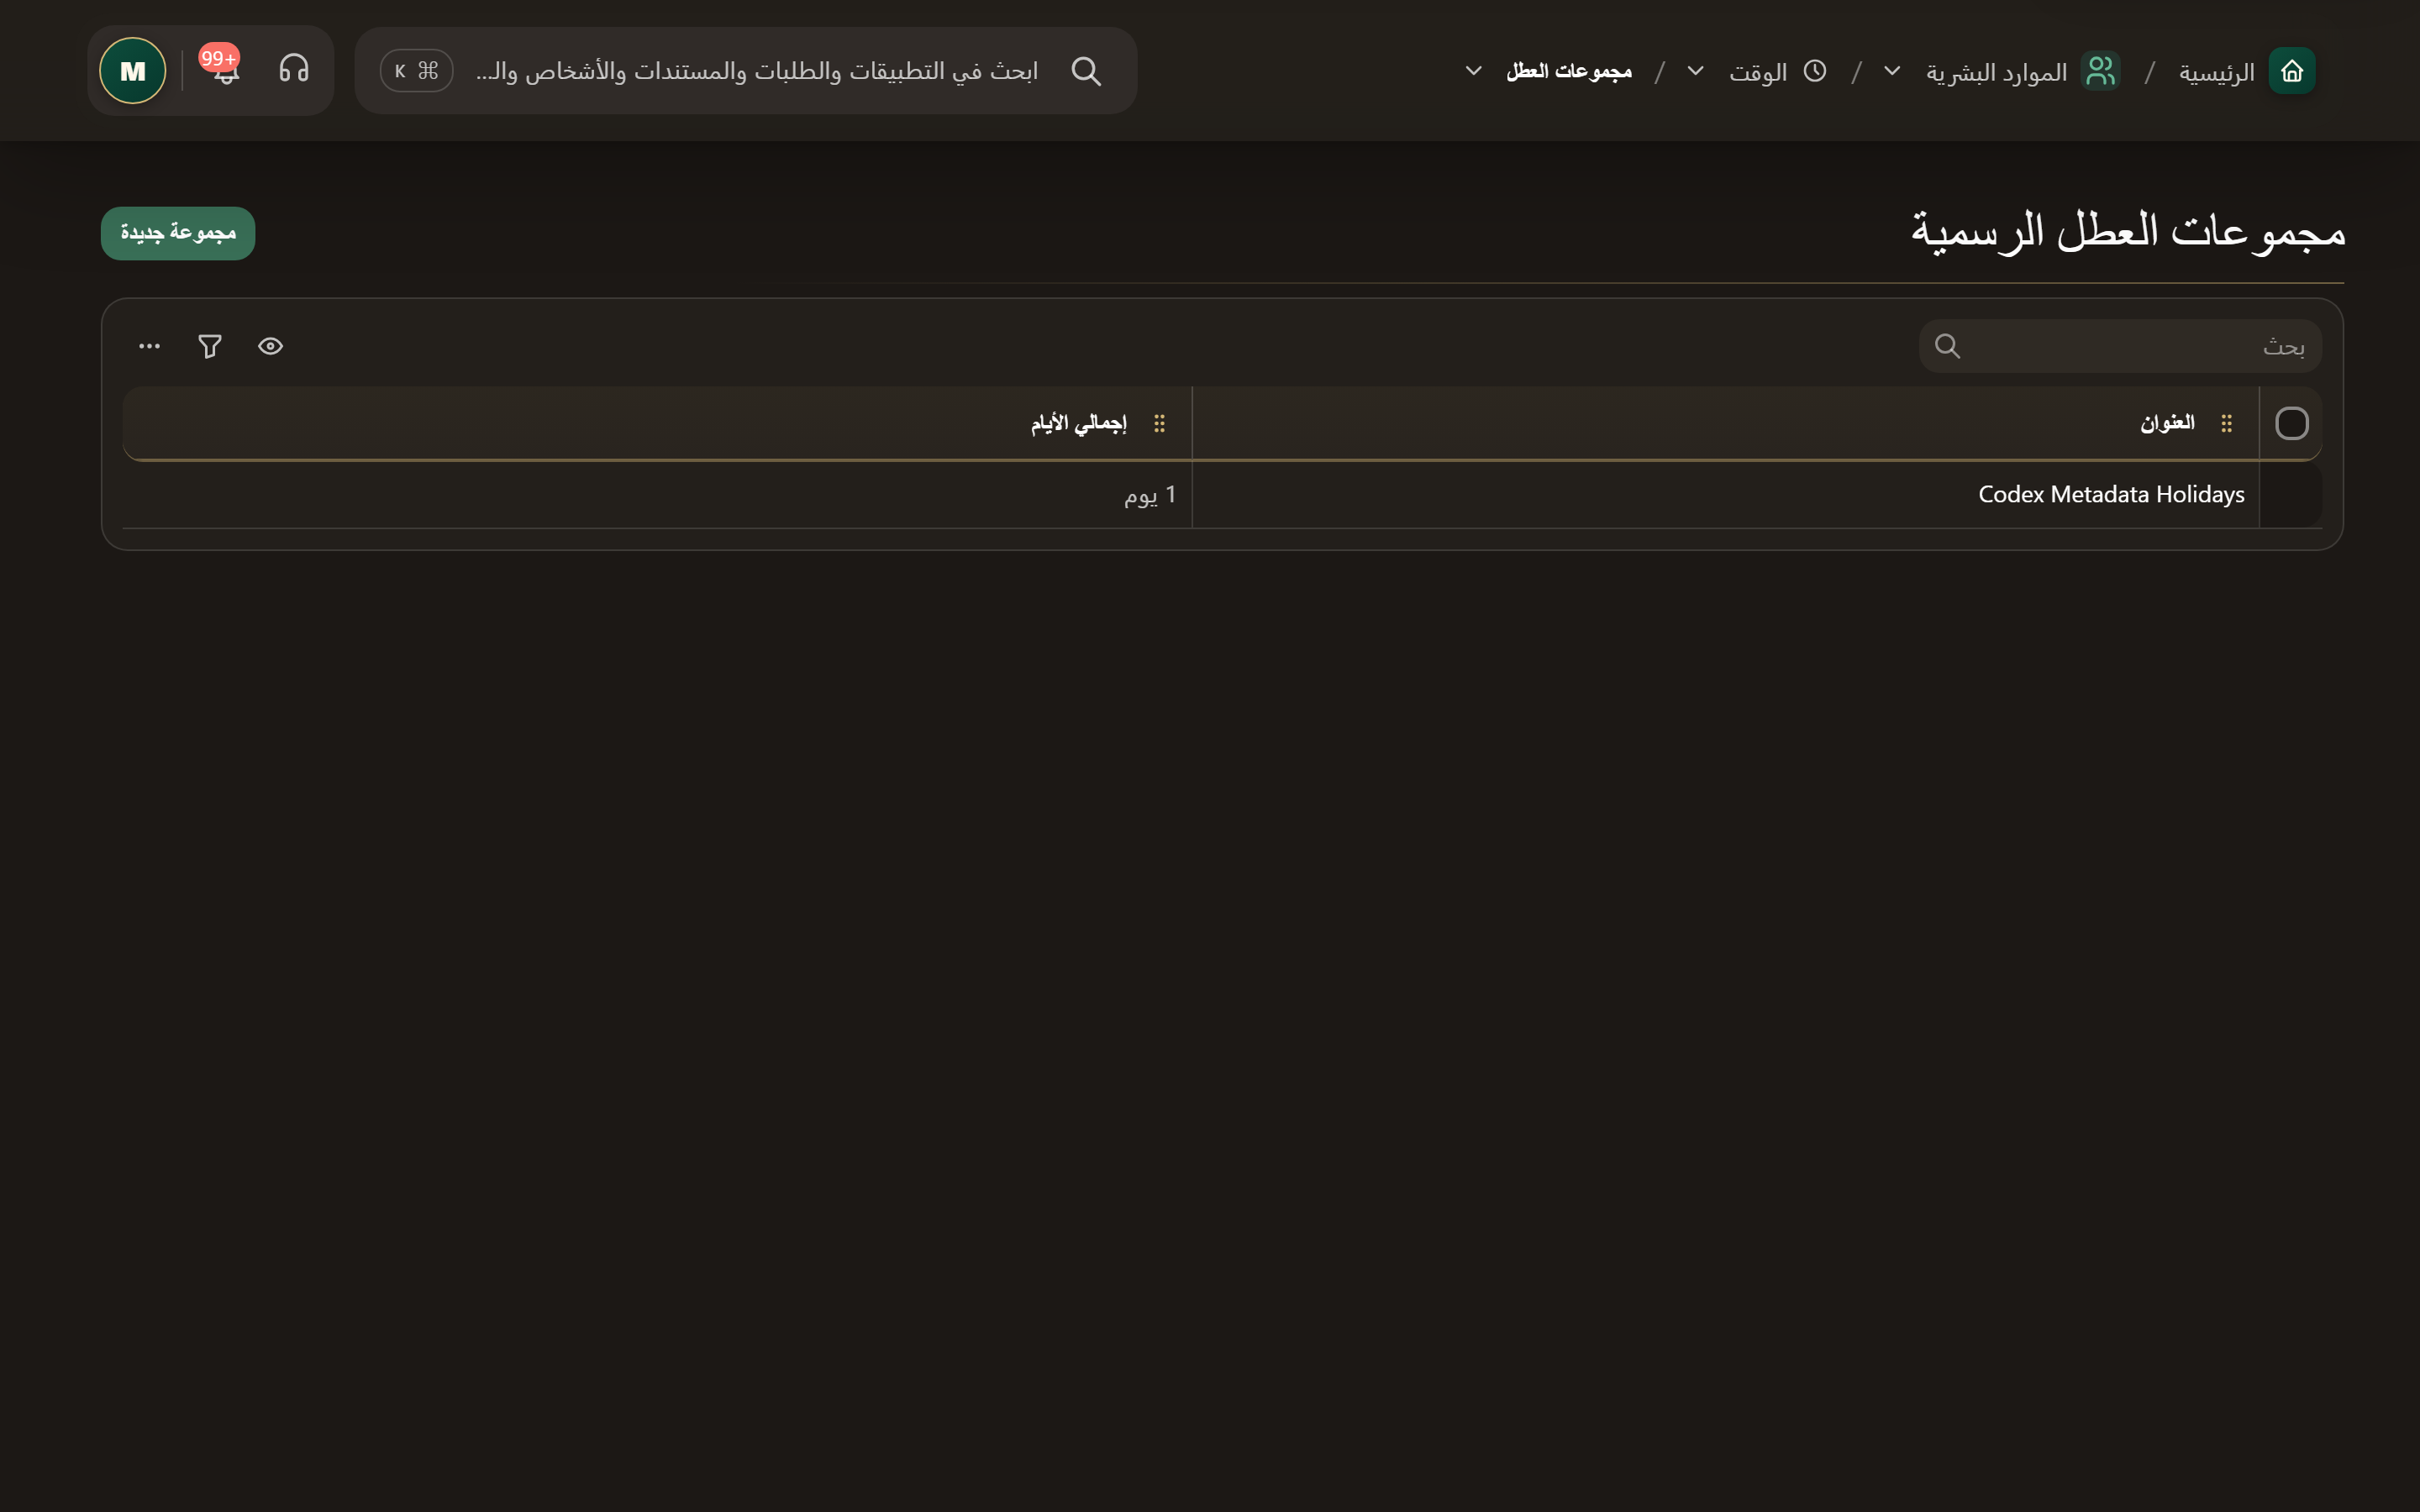
\includegraphics[width=0.95\linewidth]{figures/screens/ch03-feature-holiday-groups-ar.png}
\caption{مجموعات العطل الرسمية: الصفحة كاملة في بيئة الاختبار}
\label{fig:hr-feature-holiday-groups-screen}
\end{figure}

\begin{table}[H]
\centering
\caption{ما الذي تسجله في مجموعة العطل؟}
\label{tab:hr-feature-holiday-groups-data}
\rcZebra
\begin{tabularx}{\linewidth}{R{3.6cm} Y}
\rcHeaderRow
\thh{التبويب أو الحقل} & \thh{ما الذي تضيفه؟}\\
المجموعة & اسم المجموعة \req{}؛ عدد العطل وإجمالي الأيام \gen{}.\\
العطل & الاسم \req{}، ثم يوم كامل بتاريخه، أو يوم جزئي بساعاته، أو نطاق من تاريخ إلى تاريخ.\\
المُكلف & من يتبع المجموعة: أعضاء أو أقسام أو المؤسسة كلها.\\
\end{tabularx}
\end{table}

\begin{itemize}
  \item «مجموعة جديدة»، و«إضافة عطلة»، والبحث في العطل وتعديلها أو حذفها.
  \item لا يمكن إضافة عطلتين في التاريخ نفسه. ويمكن تحديد مجموعة عطل مختلفة في تعيين الموظف.
\end{itemize}

\begin{figure}[H]
\centering
\begin{tikzpicture}[node distance=0.5cm,stepBox/.append style={minimum width=6.5cm,text width=6.1cm,minimum height=0.8cm}]
  \node[stepBox] (a) {\RL{تجهيز التقويم المشترك}};
  \node[stepBox,below=of a] (b) {\RL{إضافة تواريخ العطل}};
  \node[stepBox,below=of b] (c) {\RL{مراجعة المُكلفين}};
  \draw[flowsTo] (a) -- (b);
  \draw[flowsTo] (b) -- (c);
\end{tikzpicture}
\rclegend
\caption{خطوات الاستخدام؛ الأسهم لا تعني معالجة تلقائية}
\label{fig:hr-feature-holiday-groups-flow}
\end{figure}

\subsection{جرّب وراجع}

\begin{enumerate}
  \item افتح «مجموعات العطل الرسمية»، ثم المجموعة المناسبة أو «مجموعة جديدة».
  \item «إضافة عطلة»: الاسم والتاريخ، واختر يوماً كاملاً أو جزئياً أو نطاقاً، ثم احفظ.
  \item في «المُكلف» اختر قسم الموارد البشرية أو المؤسسة كلها، واحفظ.
\end{enumerate}

\textbf{تحقق:} يظهر يوم العطلة بحالة «عطلة» في حضوري لكل موظف مشمول.

\clearpage
\section{تصحيحات الحضور}
\label{sec:hr-feature-attendance-corrections}

تجمع هذه الصفحة الأيام التي تحتاج تصحيحاً، مثل بصمة ناقصة، لتصحح بصماتها وتوافق على الطلب أو ترفضه.

\textbf{متى تفيد؟} لمعالجة أيام الفريق الخاطئة قبل الرواتب، بدلاً من البحث عنها يوماً بعد يوم. \textbf{المسار:} «الموارد البشرية» / «الوقت» / «تصحيحات الحضور».

\begin{figure}[H]
\centering
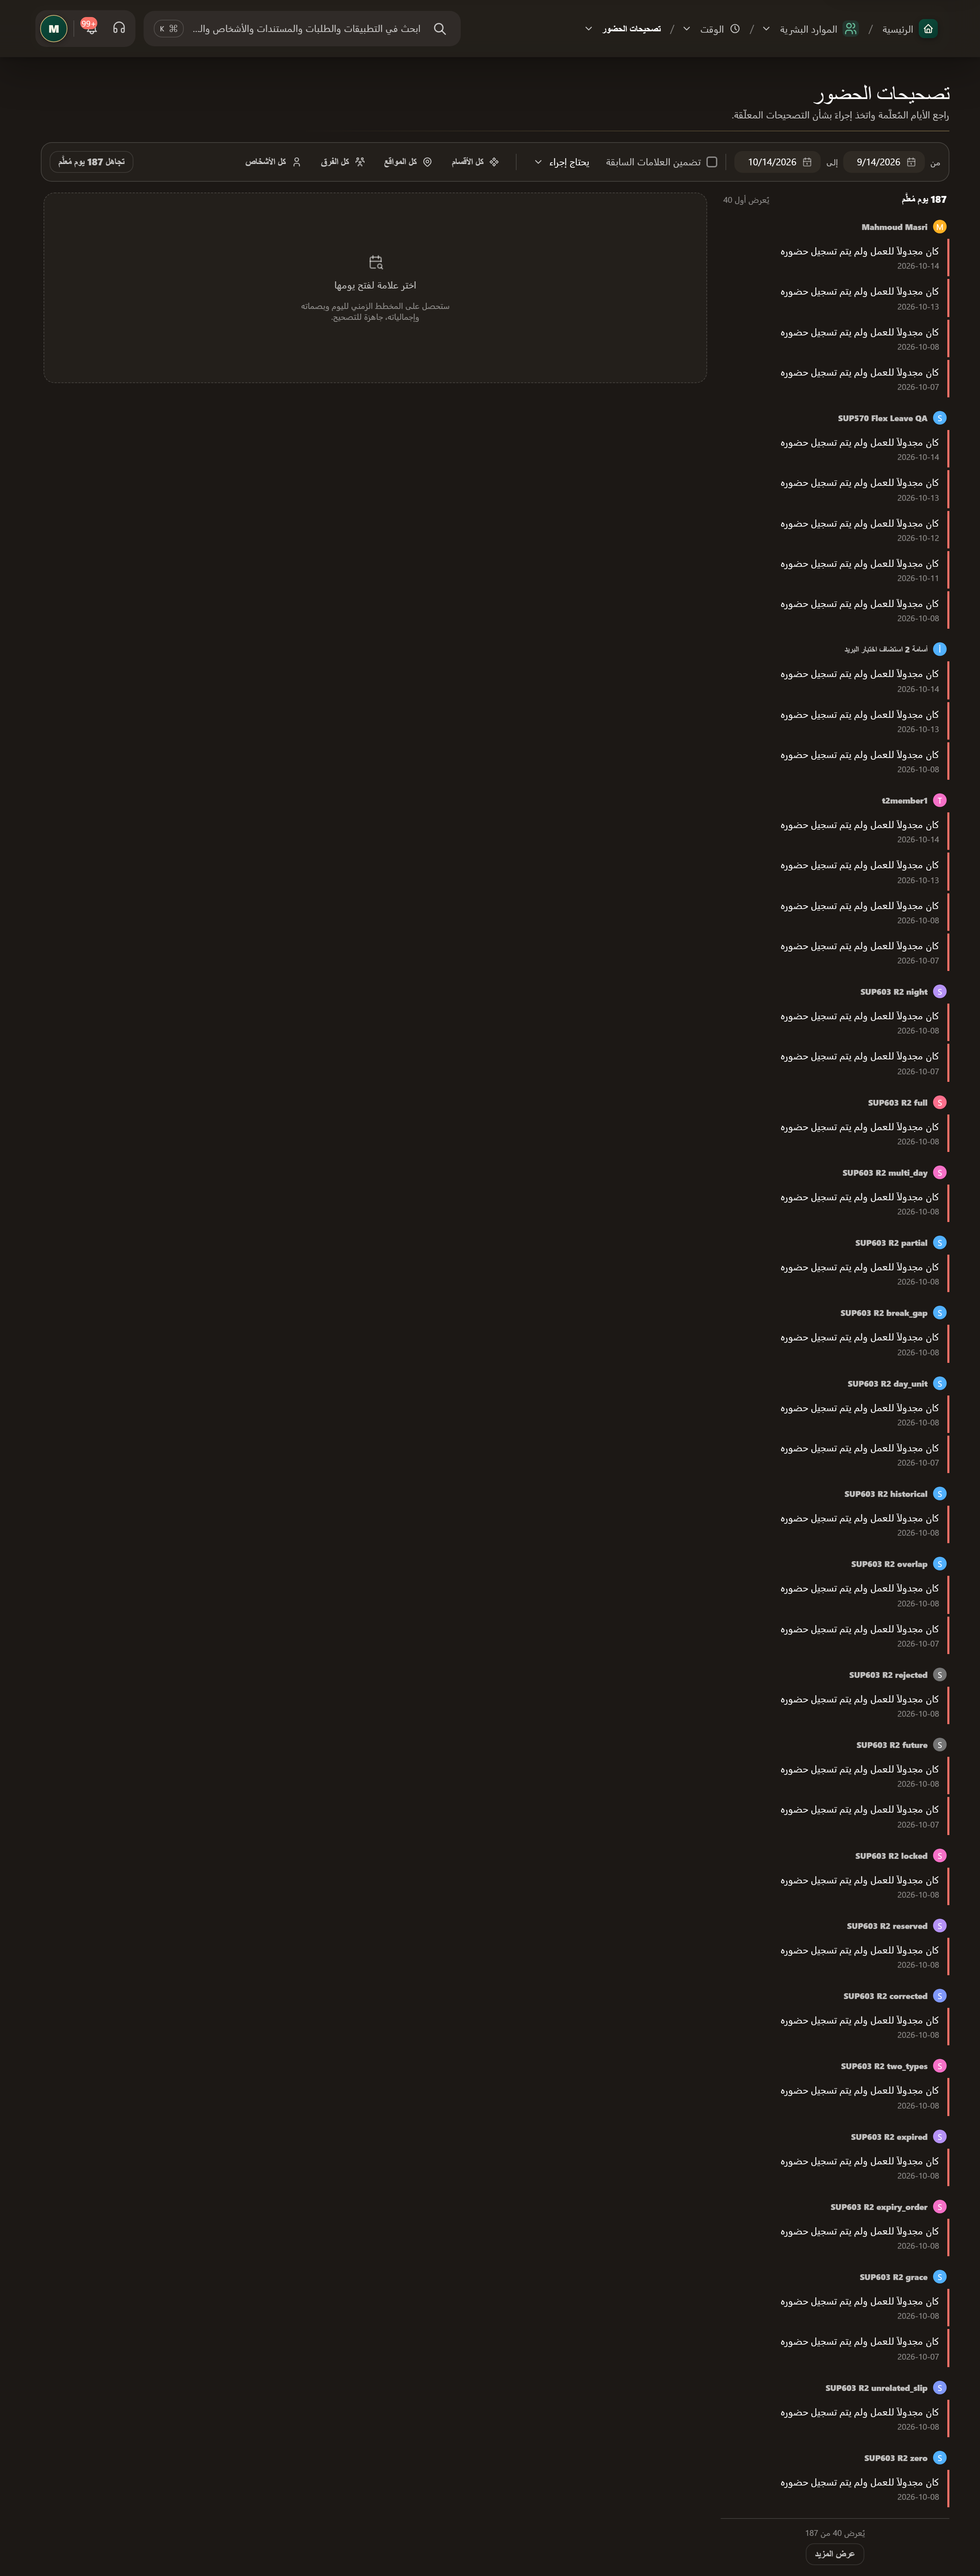
\includegraphics[width=0.95\linewidth]{figures/screens/ch03-feature-attendance-corrections-ar.png}
\caption{تصحيحات الحضور: الصفحة كاملة في بيئة الاختبار}
\label{fig:hr-feature-attendance-corrections-screen}
\end{figure}

\begin{table}[H]
\centering
\caption{ما الذي تراه في تصحيحات الحضور؟}
\label{tab:hr-feature-attendance-corrections-data}
\rcZebra
\begin{tabularx}{\linewidth}{R{3.6cm} Y}
\rcHeaderRow
\thh{الجزء} & \thh{ماذا يعرض؟}\\
التصفية & من وإلى؛ يحتاج إجراء، بانتظار الاعتماد، تمت المعالجة، الكل؛ الأقسام والمواقع والفرق والأشخاص.\\
سبب العلامة & لا انصراف، لا حضور، دخول مكرر، مدة غير منطقية، بصمة خارج الوردية، غياب في يوم مجدول.\\
لوحة اليوم & البصمات ومصدرها: جهاز أو إدخال يدوي؛ الخط الزمني؛ العمل والاستراحة مقابل الوردية.\\
الطلب & السبب والتبرير، ومن طلبه، والتغييرات، وآخر موعد للاعتماد.\\
\end{tabularx}
\end{table}

\subsection{ما الذي يمكنك فعله؟}

\begin{itemize}
  \item أضف بصمة، أو غيّر وقتها أو اتجاهها، أو احذفها. ليوم بلا بصمات: «تسجيل إجازة».
  \item «حفظ التصحيح»، «إرسال للموافقة»، «موافقة»، «رفض»؛ حسب دورك.
  \item تجاهل علامة: «تأكيد الغياب» أو «ليست مشكلة». لتجاهل عدة أيام معاً، اكتب عددها للتأكيد.
  \item مهلة التصحيح تُضبط أسفل صفحة سياسة الحضور.
\end{itemize}

\begin{figure}[H]
\centering
\begin{tikzpicture}[node distance=0.5cm,stepBox/.append style={minimum width=6.5cm,text width=6.1cm,minimum height=0.8cm}]
  \node[stepBox] (a) {\RL{مراجعة اليوم}};
  \node[stepBox,below=of a] (b) {\RL{إرسال التصحيح}};
  \node[stepBox,below=of b] (c) {\RL{مراجعة القرار واليوم}};
  \draw[flowsTo] (a) -- (b);
  \draw[flowsTo] (b) -- (c);
\end{tikzpicture}
\rclegend
\caption{خطوات الاستخدام؛ الأسهم لا تعني معالجة تلقائية}
\label{fig:hr-feature-attendance-corrections-flow}
\end{figure}

\subsection{جرّب وراجع}

\begin{enumerate}
  \item افتح «تصحيحات الحضور»، واختر «يحتاج إجراء» وقسم الموارد البشرية.
  \item افتح اليوم، وأضف البصمة الناقصة، واختر السبب، ثم «إرسال للموافقة».
\end{enumerate}

\textbf{تحقق:} ينتقل اليوم إلى «بانتظار الاعتماد»، ثم «تمت المعالجة» بعد القرار. إن لم يتوفر الإجراء، راجع المهلة والصلاحيات.

\clearpage
\section{سياسة الحضور}
\label{sec:hr-feature-attendance-policy}

تحدد سياسة الحضور كيفية تقييم الوقت المسجل: متى يُعفى الموظف من التأخر، ومتى يُحتسب الوقت عملاً إضافياً، وعلى من تنطبق القواعد.

\textbf{متى تفيد؟} مراجعة موحدة للحضور. الوردية تحدد الوقت المتوقع، والسياسة تقيّم الفرق. \textbf{المسار:} «الموارد البشرية» / «الوقت» / «سياسة الحضور».

\begin{figure}[H]
\centering
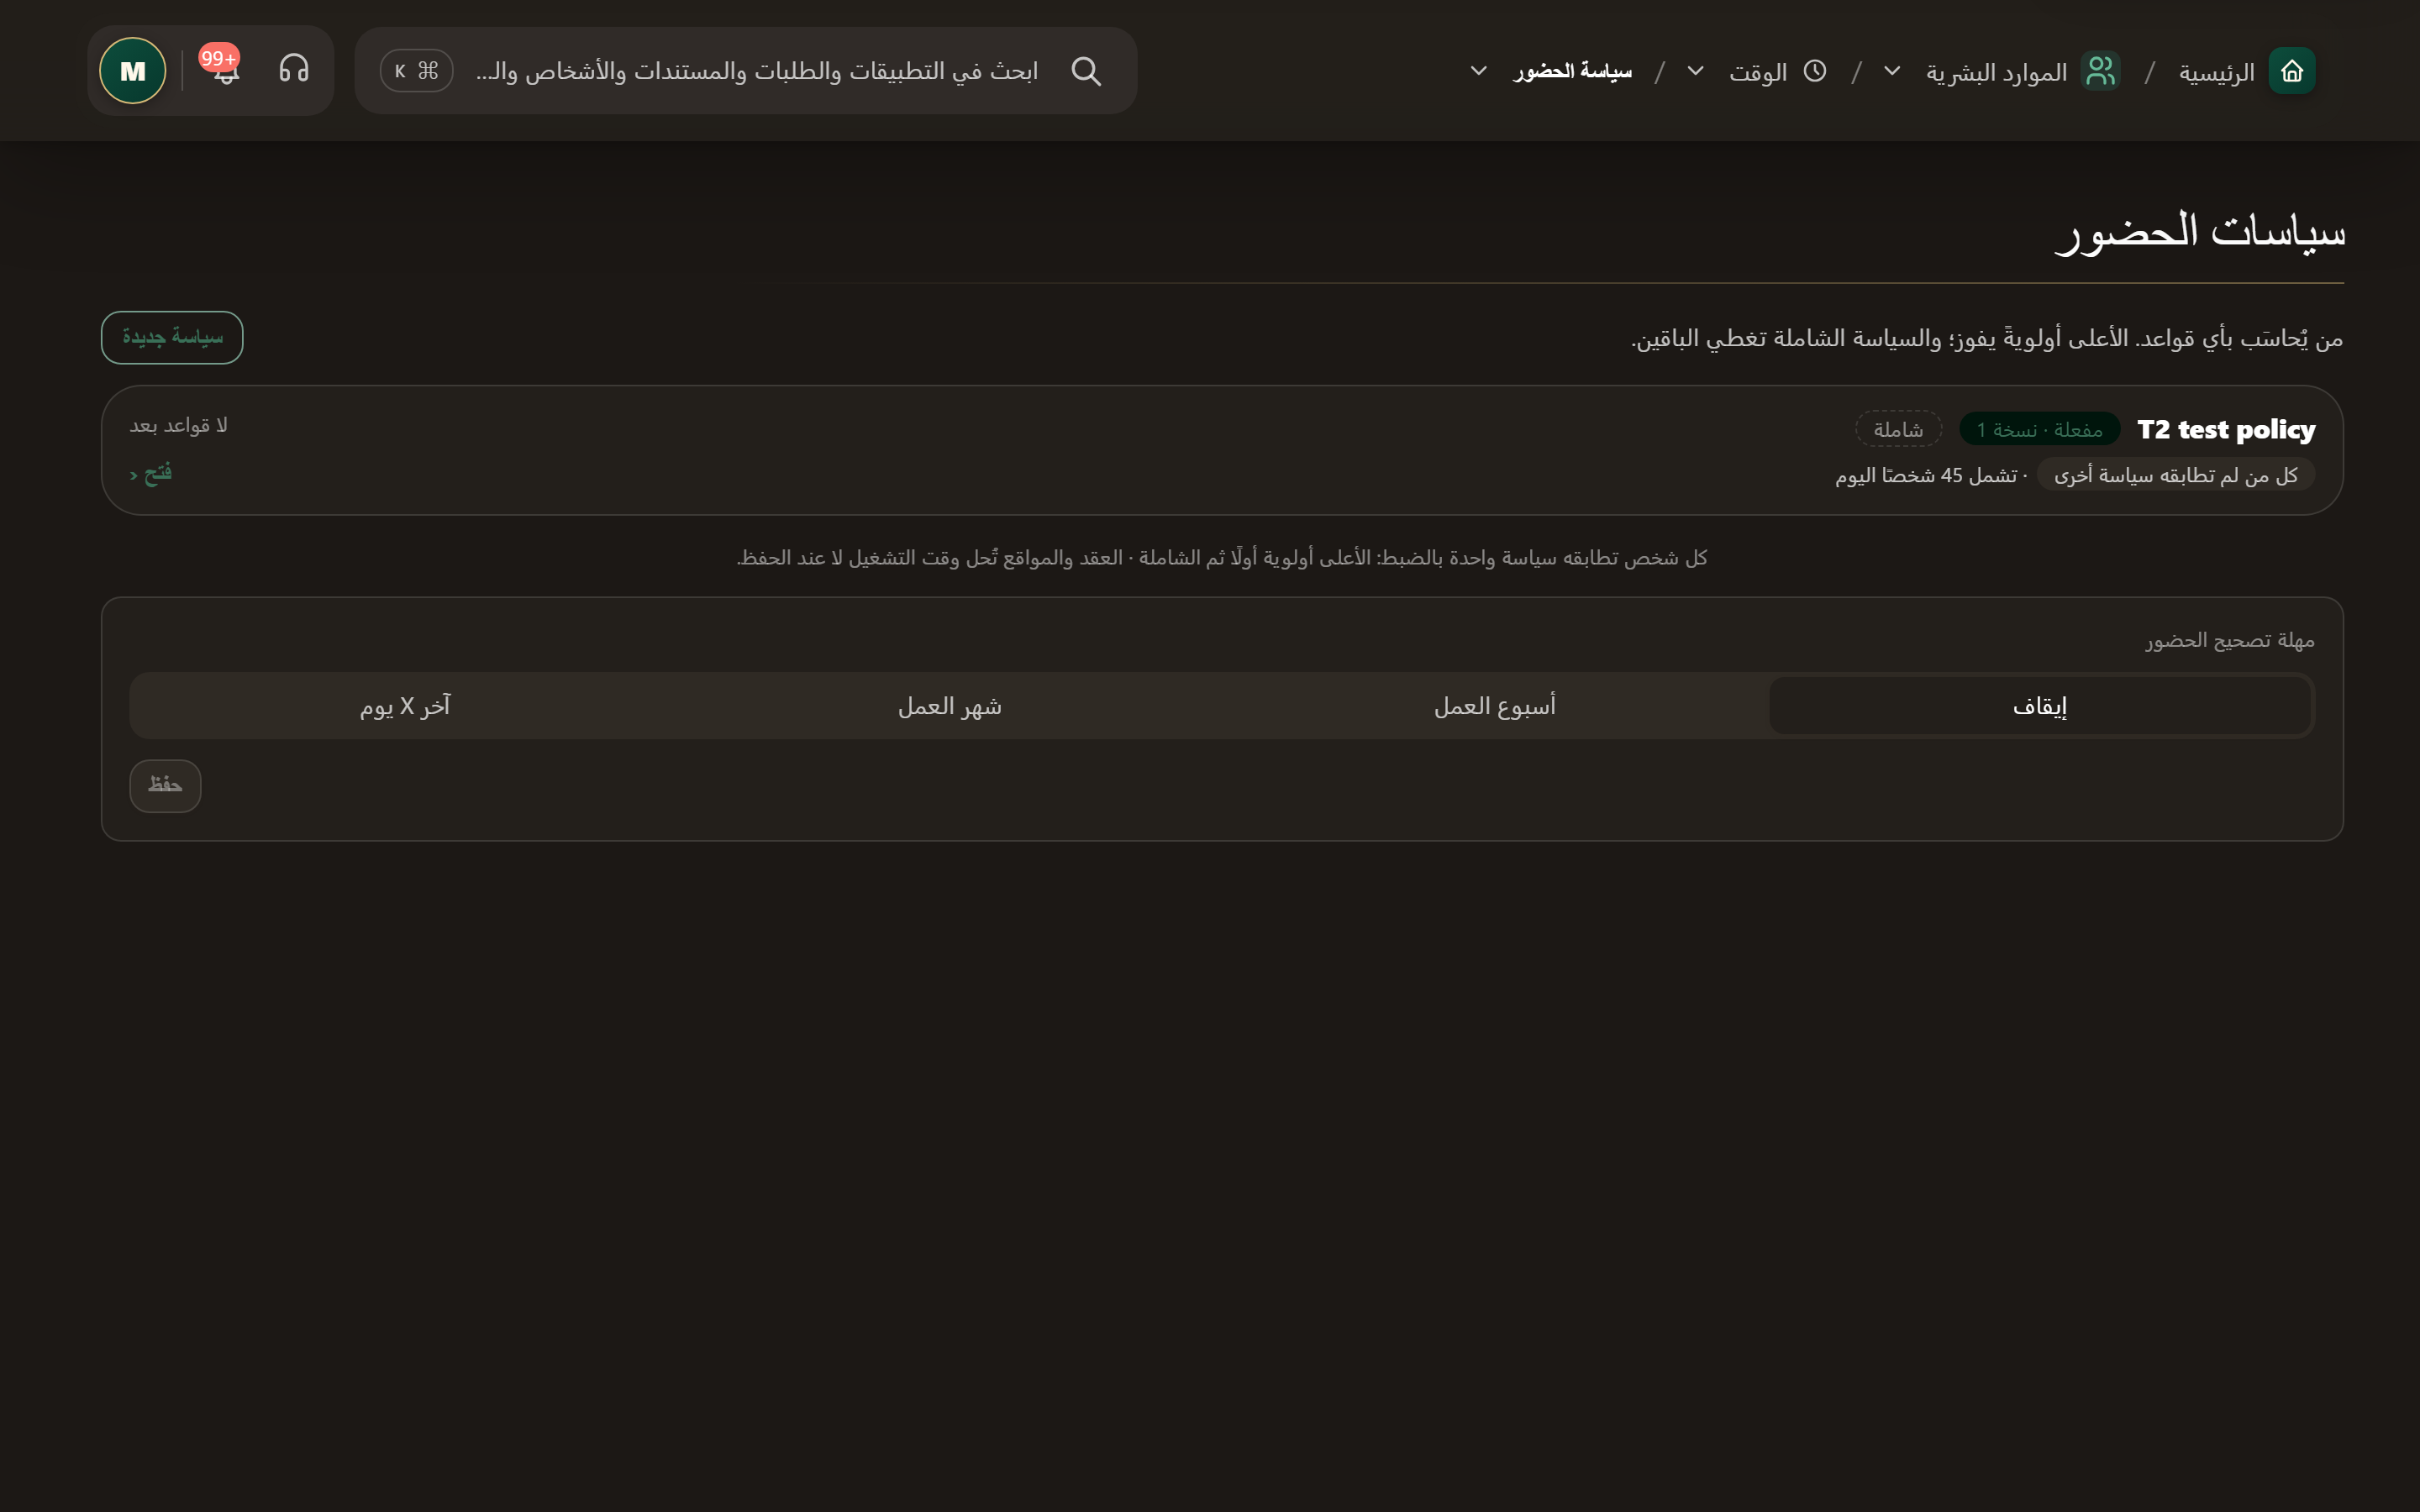
\includegraphics[width=0.95\linewidth]{figures/screens/ch03-feature-attendance-policy-ar.png}
\caption{سياسة الحضور: الصفحة كاملة في بيئة الاختبار}
\label{fig:hr-feature-attendance-policy-screen}
\end{figure}

\begin{table}[H]
\centering
\caption{ما الذي تضبطه في السياسة؟}
\label{tab:hr-feature-attendance-policy-data}
\rcZebra
\begin{tabularx}{\linewidth}{R{3.6cm} Y}
\rcHeaderRow
\thh{التبويب أو الجزء} & \thh{ما الذي تضبطه؟}\\
المسند إليهم & أشخاص أو أقسام أو مواقع أو مناصب أو مجموعات. تغطي السياسة الشاملة كل من لا تشمله سياسة أخرى.\\
قواعد بالدقائق & التأخر، المغادرة المبكرة، تجاوز الاستراحة، نقص الساعات، العمل الإضافي.\\
قواعد اليوم الكامل & الغياب، العمل في يوم الراحة، العمل في العطلة.\\
النطاقات & لكل نطاق من الدقائق (مثل \en{0–10}): يُعفى منه أو يُحتسب بمضاعف، ويُسجَّل بتصنيف مثل «تأخير مسموح».\\
الحالة & مسودة، مفعلة بإصدار، معطلة؛ وعند التعارض تُطبق السياسة الأعلى أولوية.\\
\end{tabularx}
\end{table}

\subsection{ما الذي يمكنك فعله؟}

\begin{itemize}
  \item «إنشاء سياسة»: تبدأ السياسة مسودةً، ثم «تعديل القواعد» و«حفظ المسودة» و«تفعيل».
  \item «جرّب وقتاً» للتأخر: اختر وردية ووقت وصول وشاهد النتيجة.
  \item «محاكاة»: «إعادة احتساب الشهر الماضي» بالمسودة قبل تفعيلها.
  \item «تعطيل السياسة»، و«حذف السياسة» إن لم تُفعّل قط.
\end{itemize}

\begin{figure}[H]
\centering
\begin{tikzpicture}[node distance=0.5cm,stepBox/.append style={minimum width=6.5cm,text width=6.1cm,minimum height=0.8cm}]
  \node[stepBox] (a) {\RL{اختيار المشمولين بالسياسة}};
  \node[stepBox,below=of a] (b) {\RL{مراجعة قواعد الحضور}};
  \node[stepBox,below=of b] (c) {\RL{فحص نتيجة تجريبية}};
  \draw[flowsTo] (a) -- (b);
  \draw[flowsTo] (b) -- (c);
\end{tikzpicture}
\rclegend
\caption{خطوات الاستخدام؛ الأسهم لا تعني معالجة تلقائية}
\label{fig:hr-feature-attendance-policy-flow}
\end{figure}

\subsection{جرّب وراجع}

\begin{enumerate}
  \item يفتح المسؤول المخوّل «سياسة الحضور» ويختار السياسة، ثم «تعديل القواعد».
  \item في التأخر أضف نطاقاً: من \en{0} إلى \en{10} دقائق يُعفى منه. احفظ المسودة.
  \item استخدم «جرّب وقتاً» و«محاكاة»، ثم «تفعيل» عند صحة النتيجة.
\end{enumerate}

\textbf{تحقق:} راجع يوماً فعلياً في حضوري بعد التفعيل. علامة تنبيه وحدها لا تعني خصماً من الراتب.

\clearpage
\section{أجهزة الحضور}
\label{sec:hr-feature-attendance-terminals}

تربط هذه الصفحة أجهزة البصمة بالنظام. لكل موقع شبكة يعمل فيها برنامج اتصال يسمى «وكيل الحضور»، ويرسل البصمات تلقائياً، ثم تُطابق البصمات مع الأعضاء.

\textbf{متى تفيد؟} عندما يأتي الحضور من جهاز فعلي. وجود الجهاز في القائمة لا يثبت وصول بصماته. \textbf{المسار:} «الموارد البشرية» / «الوقت» / «أجهزة الحضور».

\begin{figure}[H]
\centering
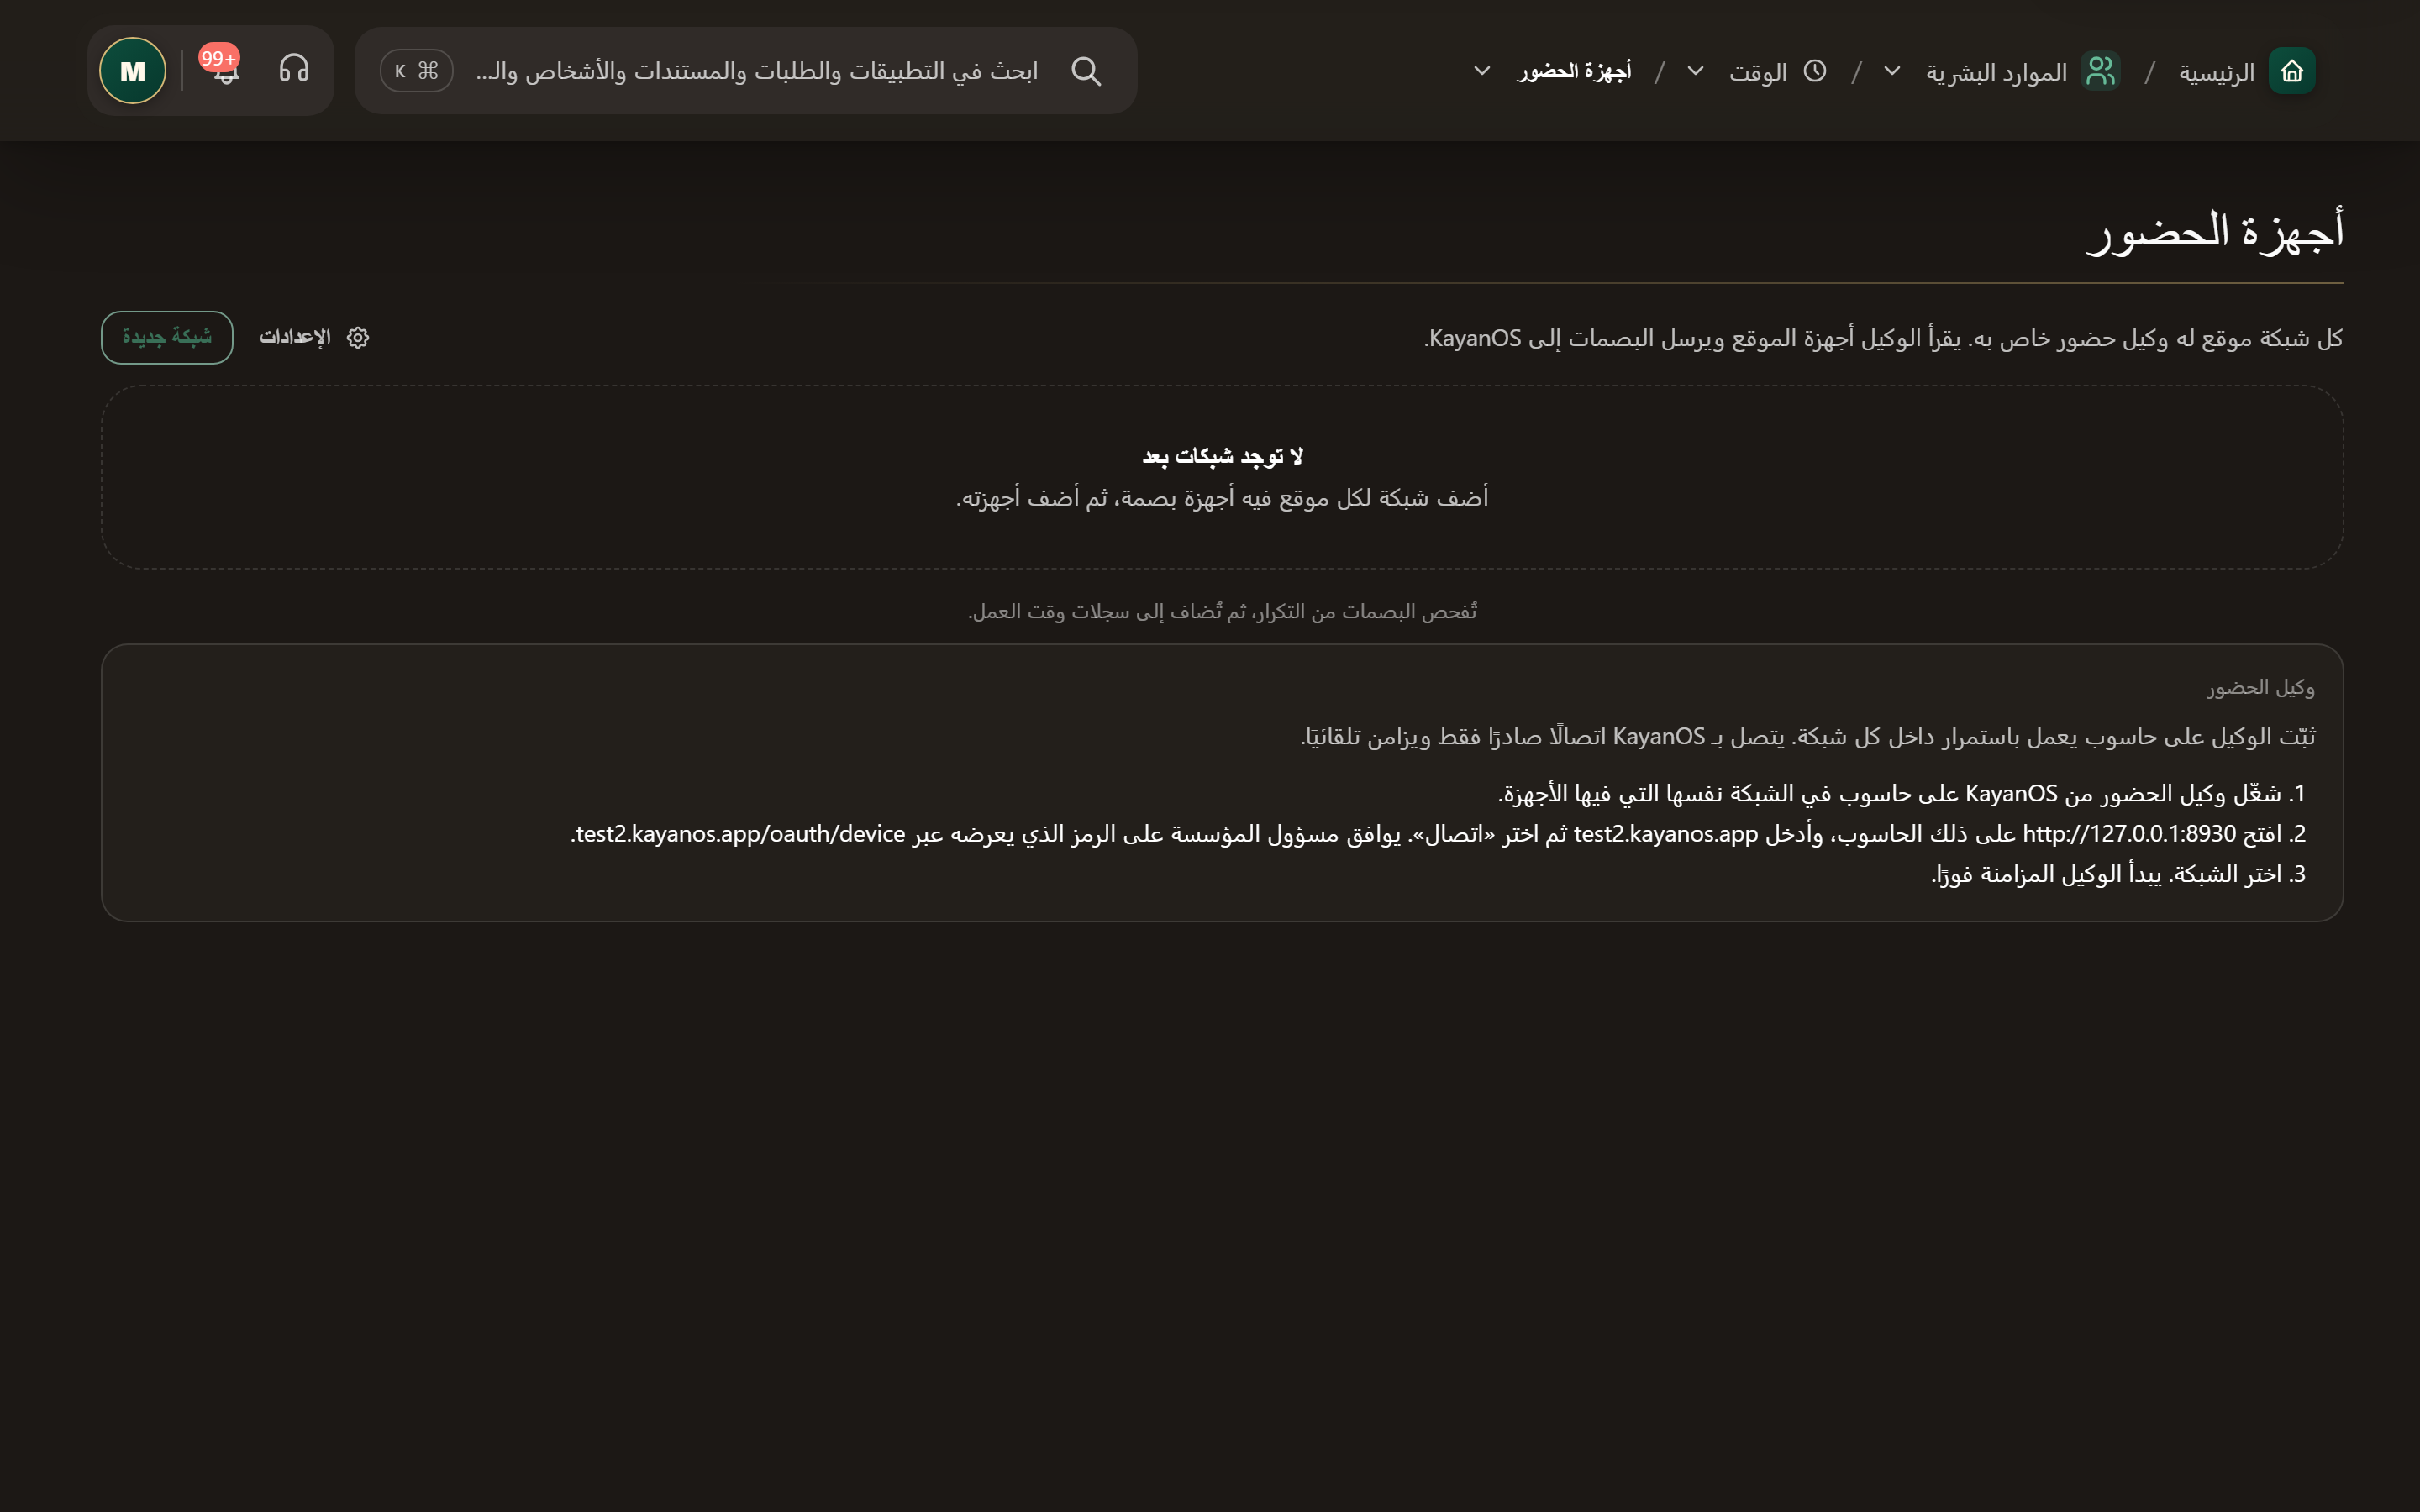
\includegraphics[width=0.95\linewidth]{figures/screens/ch03-feature-attendance-terminals-ar.png}
\caption{أجهزة الحضور: الصفحة كاملة في بيئة الاختبار}
\label{fig:hr-feature-attendance-terminals-screen}
\end{figure}

\begin{table}[H]
\centering
\caption{ما الذي تسجله في أجهزة الحضور؟}
\label{tab:hr-feature-attendance-terminals-data}
\rcZebra
\begin{tabularx}{\linewidth}{R{3.6cm} Y}
\rcHeaderRow
\thh{الجزء} & \thh{ما الذي تضيفه أو تراه؟}\\
الشبكة & الاسم \req{}، الموقع، المنطقة الزمنية، فاصل المزامنة (من \en{5} إلى \en{60} دقيقة).\\
الجهاز & الاسم وعنوان \en{IP} والمنفذ \req{} (\en{4370} افتراضياً)، مفتاح الاتصال، اتجاه البصمة.\\
تفاصيل الجهاز & الطراز، المستخدمون المسجلون، السعة، ساعة الجهاز وفارق توقيتها، آخر بصمة \gen{}.\\
الإعدادات & استيراد البصمات بدءاً من تاريخ، ومطابقة تلقائية برقم الموظف أو يدوية.\\
\end{tabularx}
\end{table}

\subsection{ما الذي يمكنك فعله؟}

\begin{itemize}
  \item «شبكة جديدة»، ثم «إضافة جهاز».
  \item تبويبات الشبكة: الأجهزة، عمليات المزامنة، بصمات غير مطابقة مع «ربط بعضو»، الوكيل مع «قطع اتصال الوكيل».
  \item المزامنة يجريها الوكيل؛ لا يوجد زر مزامنة يدوية.
\end{itemize}

\begin{figure}[H]
\centering
\begin{tikzpicture}[node distance=0.5cm,stepBox/.append style={minimum width=6.5cm,text width=6.1cm,minimum height=0.8cm}]
  \node[stepBox] (a) {\RL{فحص الجهاز}};
  \node[stepBox,below=of a] (b) {\RL{مطابقة المستخدمين}\\\RL{بالأعضاء}};
  \node[stepBox,below=of b] (c) {\RL{مراجعة بصمة حضور}};
  \draw[flowsTo] (a) -- (b);
  \draw[flowsTo] (b) -- (c);
\end{tikzpicture}
\rclegend
\caption{خطوات الاستخدام؛ الأسهم لا تعني معالجة تلقائية}
\label{fig:hr-feature-attendance-terminals-flow}
\end{figure}

\subsection{جرّب وراجع}

\begin{enumerate}
  \item يفتح المسؤول المخوّل «أجهزة الحضور» ثم شبكة الموقع. للموقع الجديد: «شبكة جديدة» ثم «إضافة جهاز».
  \item راجع حالة الوكيل وآخر مزامنة. في «بصمات غير مطابقة» اربط كل مستخدم على الجهاز بالعضو المقابل له.
\end{enumerate}

\textbf{تحقق:} قارن بصمة معروفة بيوم الموظف في حضوري. إن غابت، افحص الوكيل والمطابقة والمنطقة الزمنية.

\clearpage
\section{المستويات الوظيفية}
\label{sec:hr-feature-seniority-levels}

المستوى الوظيفي درجة في سلم الراتب، لها رتبة، وحدّ أدنى وأعلى للراتب، ومجموعة خبرة.

\textbf{متى تفيد؟} مرجع موحد للتعويض: لكل منصب درجة. الدرجة لا تخص موظفاً بعينه، وليست قسيمة راتب. \textbf{المسار:} «الموارد البشرية» / «سلم الراتب» / «المستويات الوظيفية».

\begin{figure}[H]
\centering
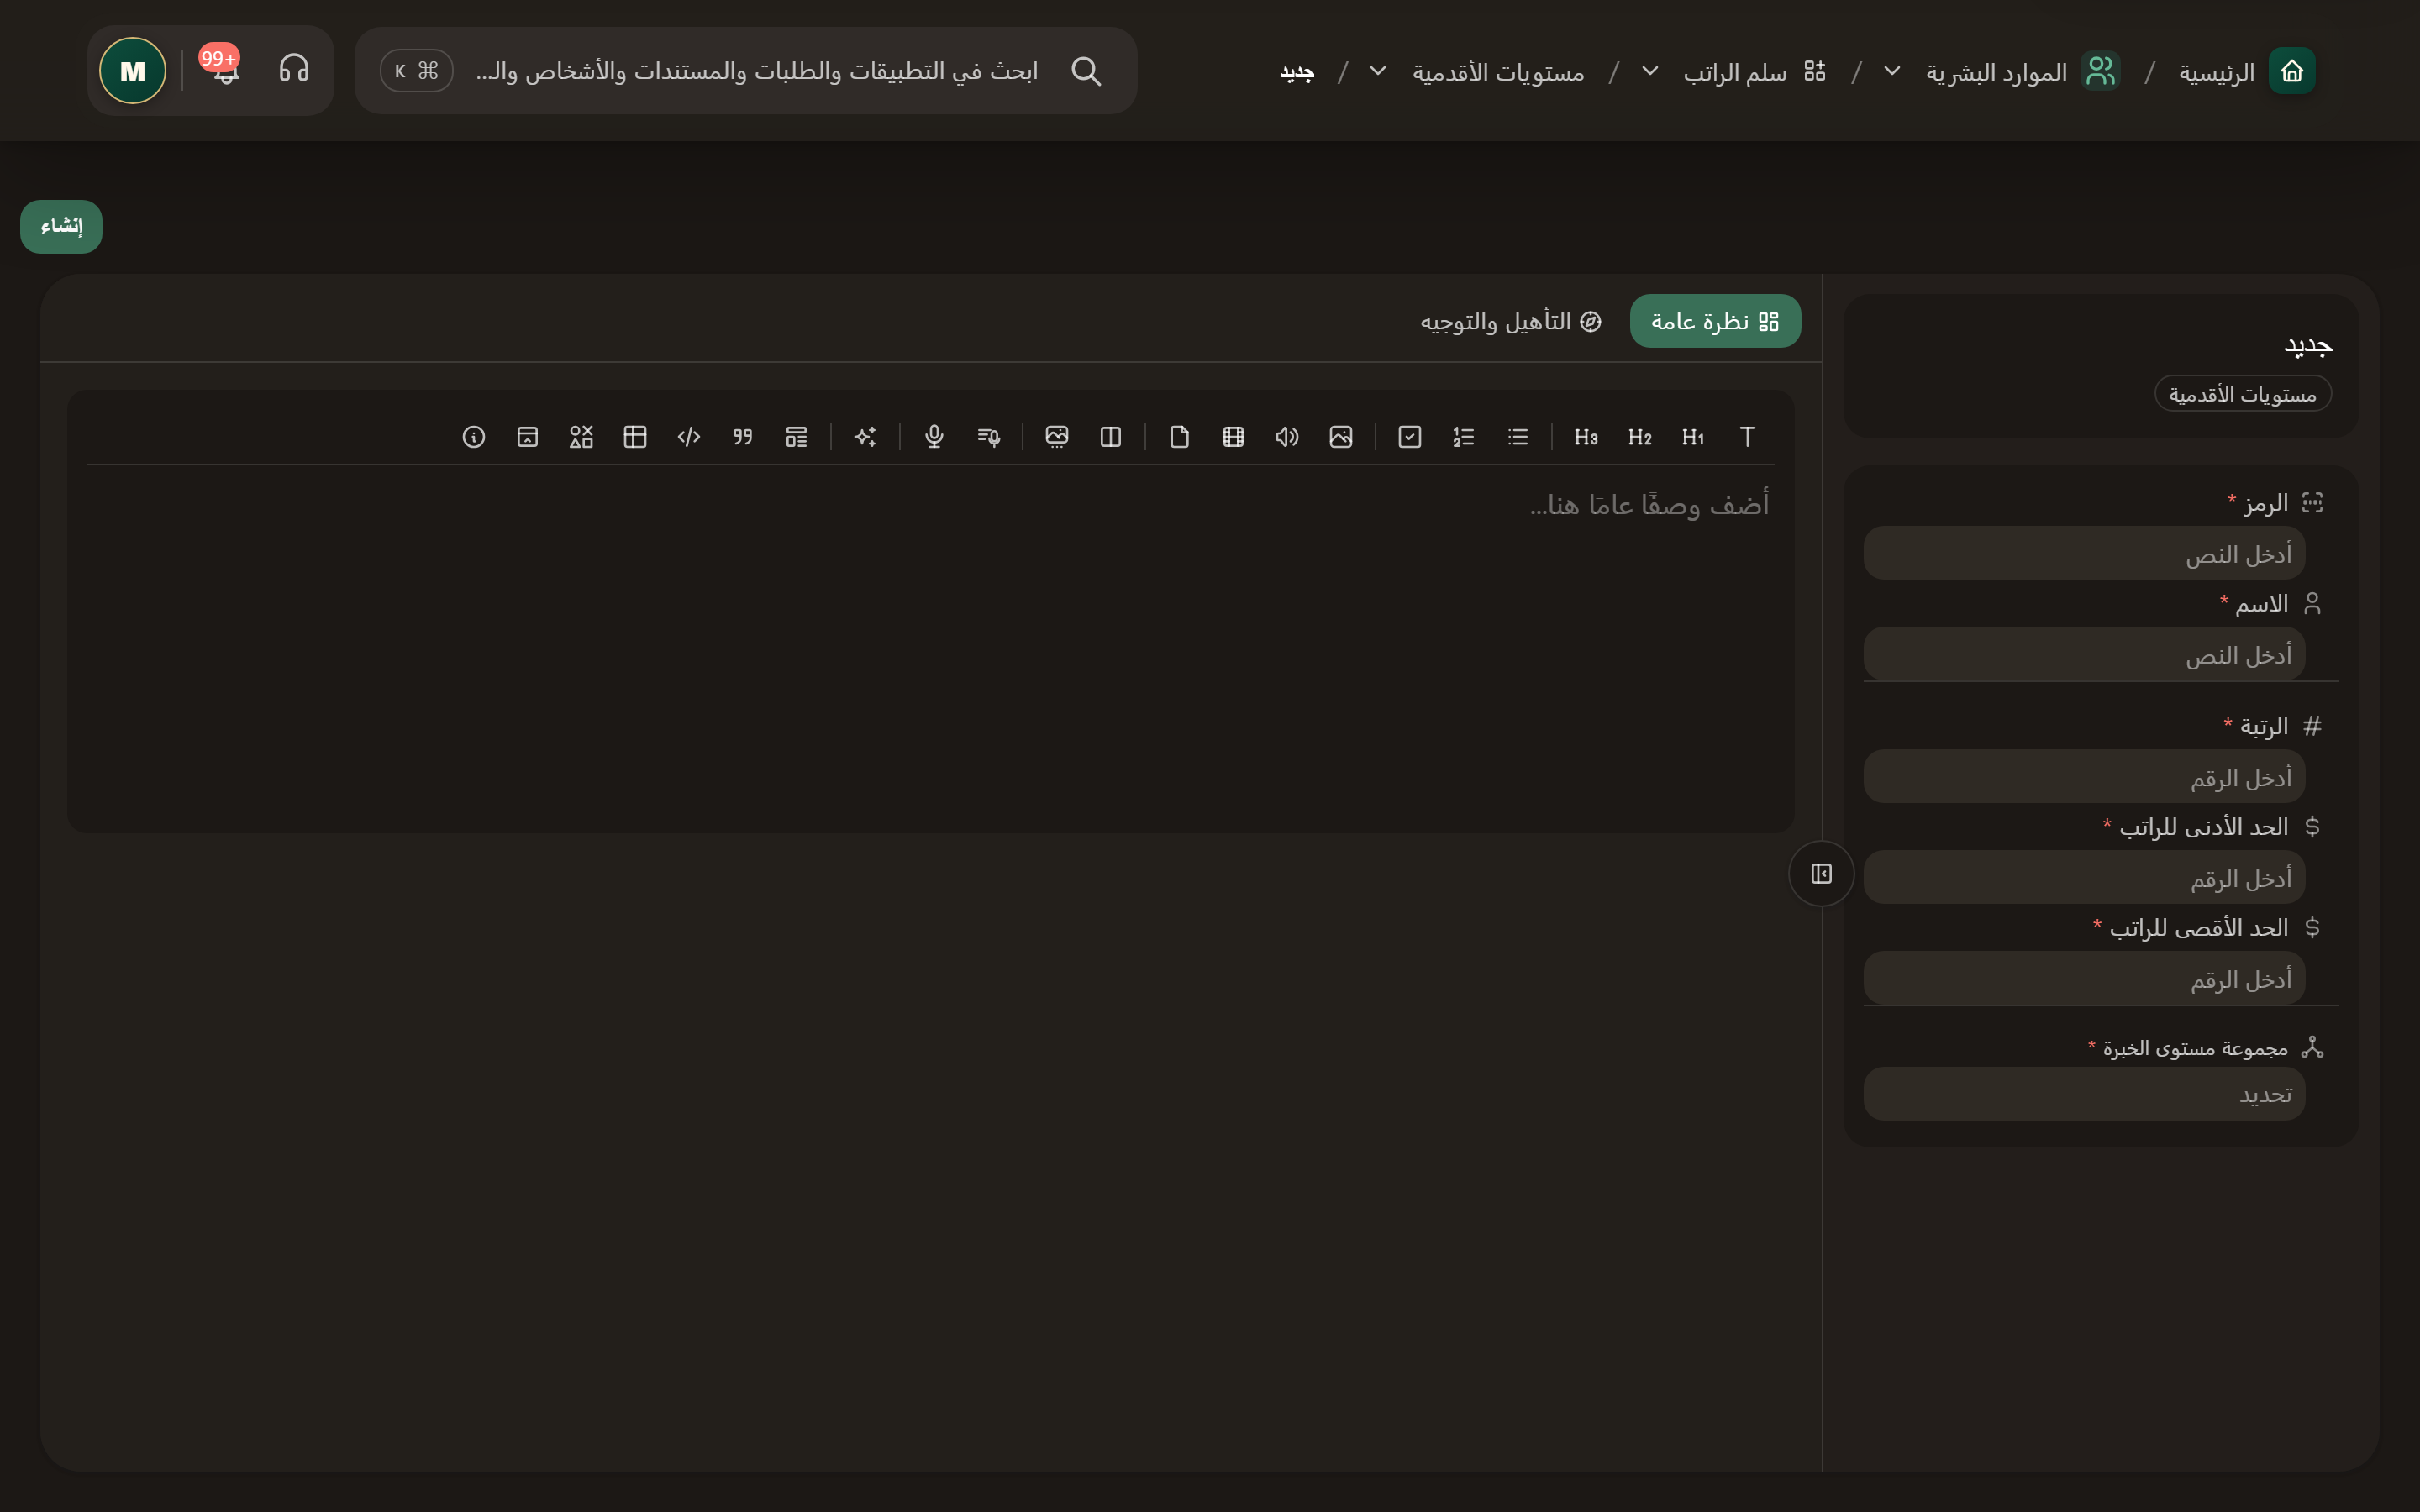
\includegraphics[width=0.95\linewidth]{figures/screens/ch03-feature-seniority-levels-ar.png}
\caption{المستويات الوظيفية: نموذج غير محفوظ في بيئة الاختبار}
\label{fig:hr-feature-seniority-levels-screen}
\end{figure}

\begin{table}[H]
\centering
\caption{ما الذي تسجله في المستوى الوظيفي؟}
\label{tab:hr-feature-seniority-levels-data}
\rcZebra
\begin{tabularx}{\linewidth}{R{3.6cm} Y}
\rcHeaderRow
\thh{الحقل} & \thh{ما الذي تضيفه؟}\\
الاسم والرمز & \req{}؛ الرمز لا يتكرر.\\
الرتبة & \req{}: رقم فريد يرتب الدرجات.\\
الراتب المبدئي والحد الأقصى & \req{}: أدنى راتب في الدرجة وأعلاه.\\
مجموعة مستويات الخبرة & \req{}: الزيادات التي تُضاف إلى الراتب المبدئي.\\
\end{tabularx}
\end{table}

يرتبط المنصب بمستوى وظيفي. يقترح النظام راتب التعيين من الراتب المبدئي وزيادات الخبرة \gen{}.

\begin{figure}[H]
\centering
\begin{tikzpicture}[node distance=0.5cm,stepBox/.append style={minimum width=6.5cm,text width=6.1cm,minimum height=0.8cm}]
  \node[stepBox] (a) {\RL{تعريف الدرجة الوظيفية}};
  \node[stepBox,below=of a] (b) {\RL{مراجعة سلم الراتب}};
  \node[stepBox,below=of b] (c) {\RL{فحص راتب التعيين}};
  \draw[flowsTo] (a) -- (b);
  \draw[flowsTo] (b) -- (c);
\end{tikzpicture}
\rclegend
\caption{خطوات الاستخدام؛ الأسهم لا تعني معالجة تلقائية}
\label{fig:hr-feature-seniority-levels-flow}
\end{figure}

\subsection{جرّب وراجع}

\begin{enumerate}
  \item جهّز مجموعة الخبرة أولاً. افتح «المستويات الوظيفية» وأضف المستوى الوظيفي.
  \item أكمل الاسم والرمز والرتبة والراتب المبدئي والحد الأقصى ومجموعة الخبرة بالقيم المعتمدة، ثم احفظ.
\end{enumerate}

\textbf{تحقق:} افتح «سلم الراتب» وراجع صف الدرجة. اربط الدرجة بالمنصب، ثم راجع راتب التعيين.

\clearpage
\section{مستويات الخبرة}
\label{sec:hr-feature-experience-levels}

تدير في هذه الصفحة مجموعات الخبرة: لكل مجموعة مستويات مرتبة، وقاعدة تزيد الراتب من مستوى إلى المستوى الذي يليه.

\textbf{متى تفيد؟} زيادات خبرة موحدة في سلم الراتب. العبرة بترتيب المستويات؛ تغيير اسم المستوى لا يغير مكانه. \textbf{المسار:} «الموارد البشرية» / «سلم الراتب» / «مستويات الخبرة».

\begin{figure}[H]
\centering
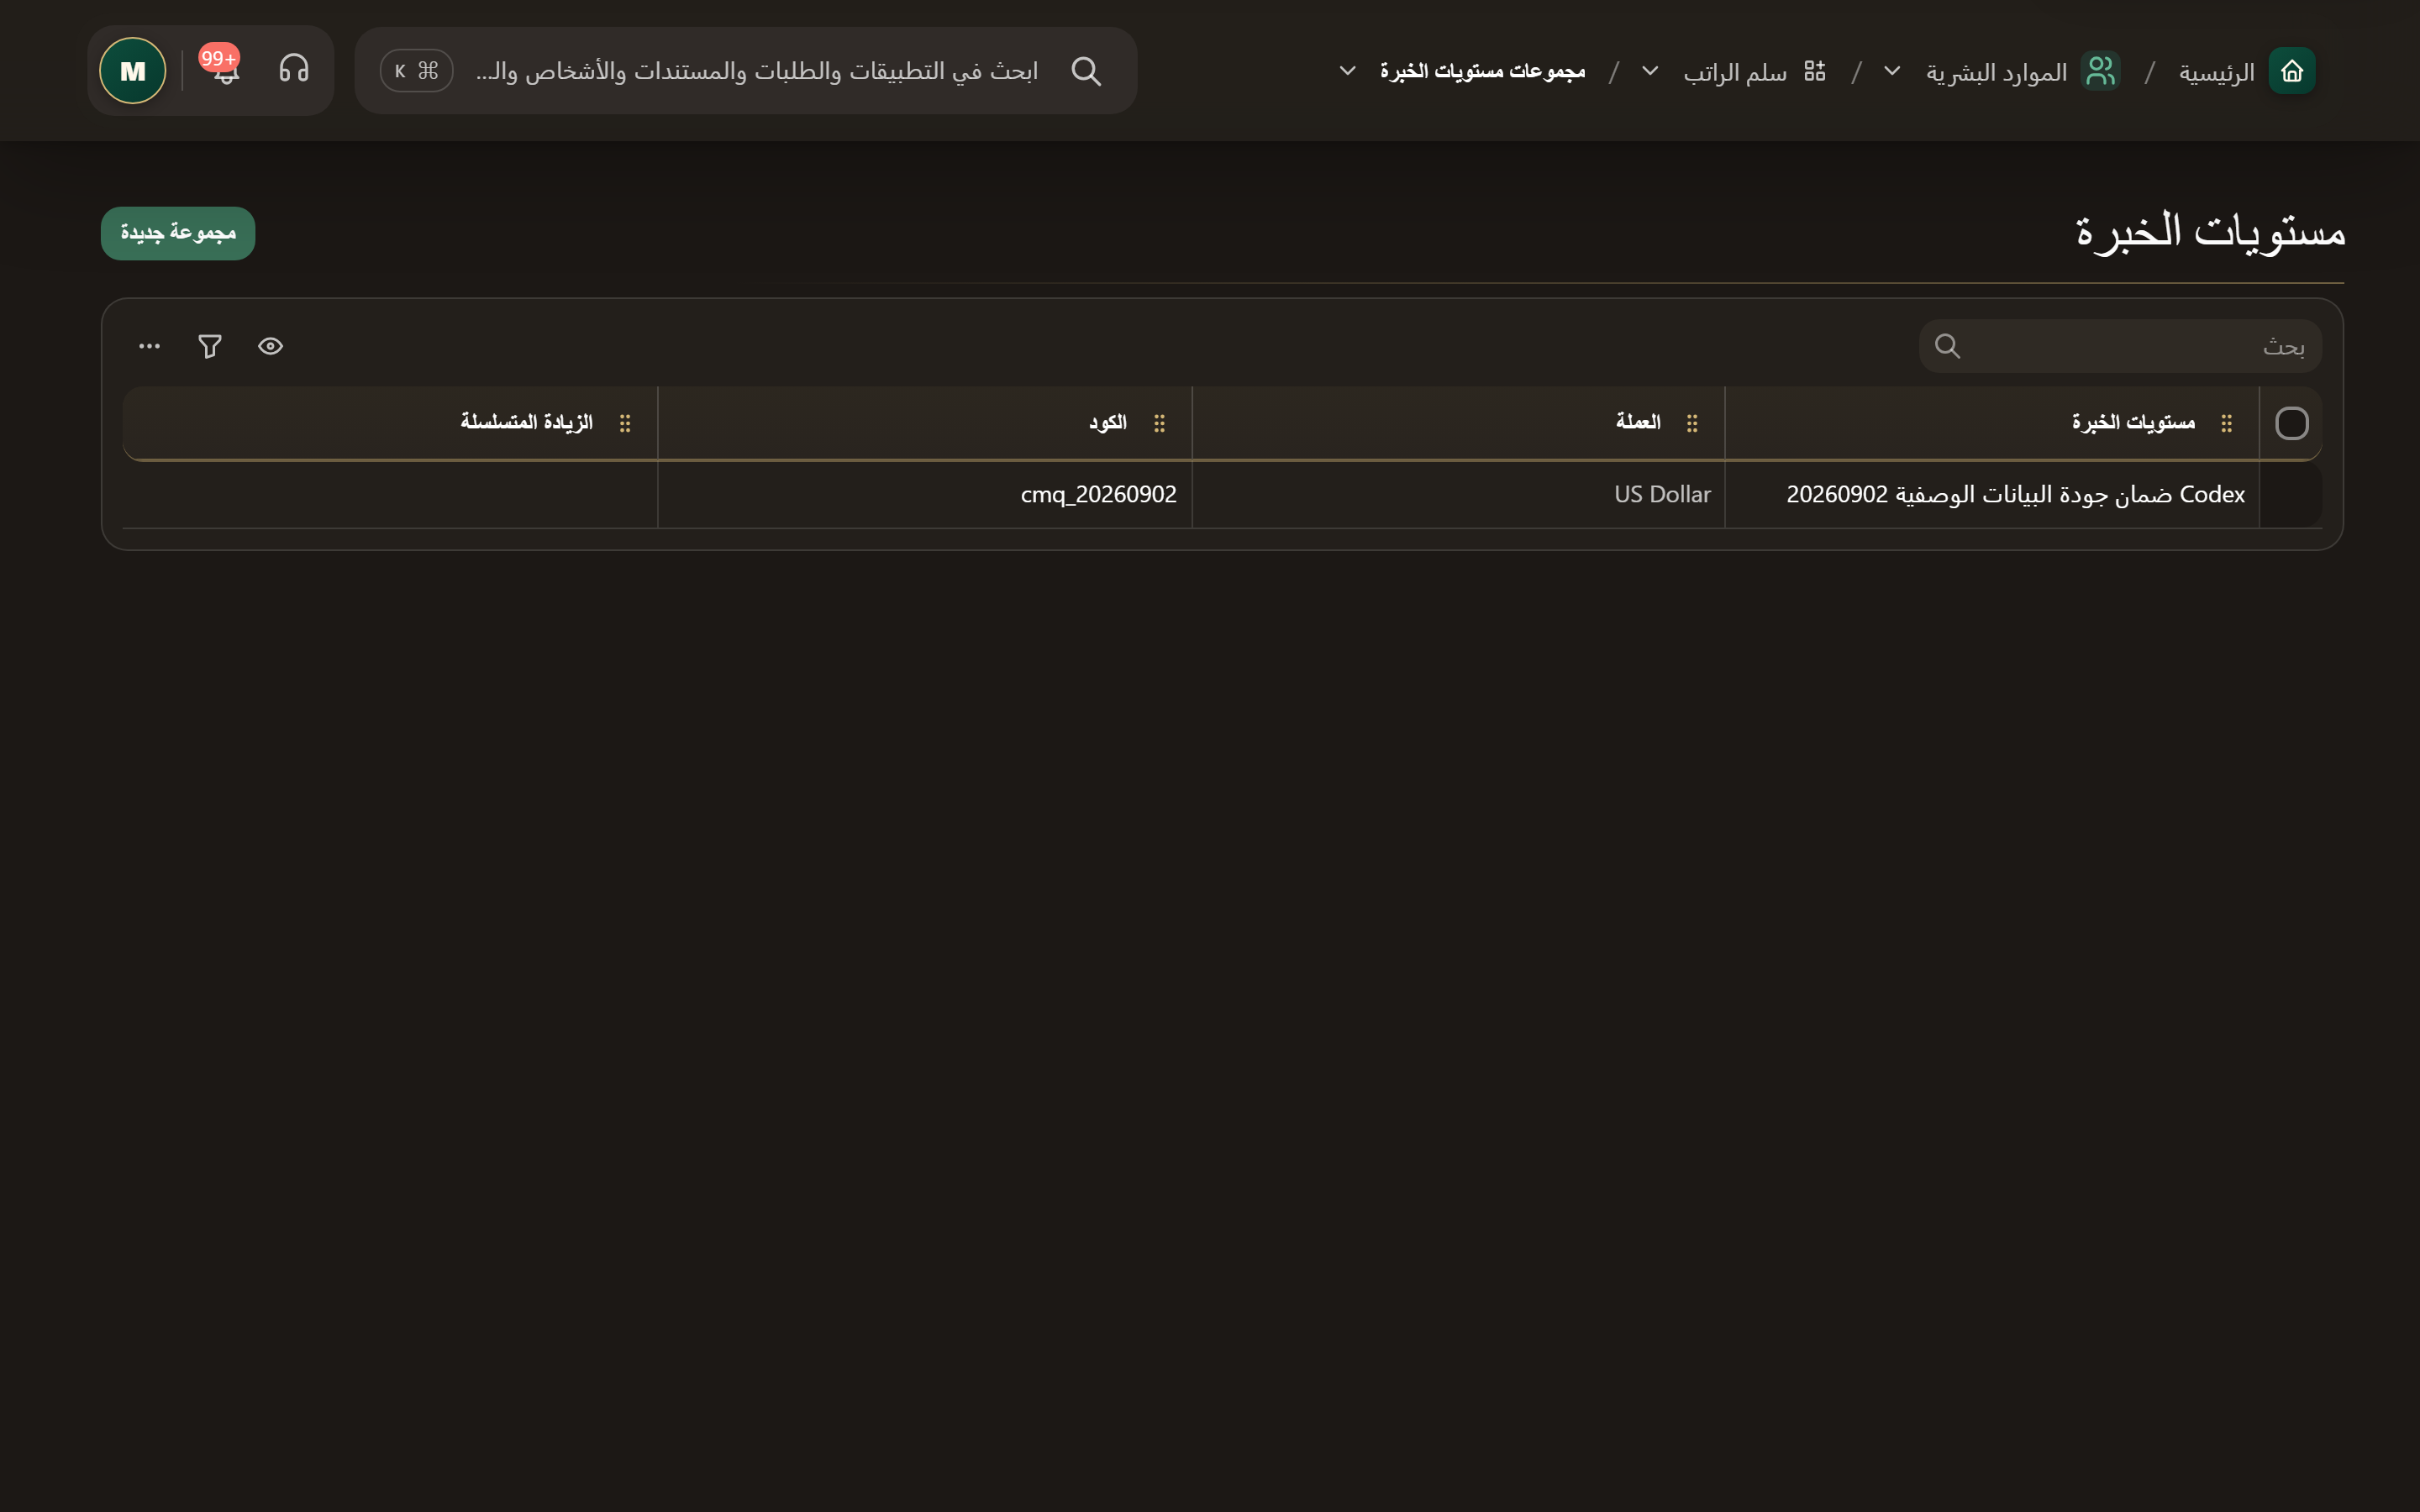
\includegraphics[width=0.95\linewidth]{figures/screens/ch03-feature-experience-levels-ar.png}
\caption{مستويات الخبرة: الصفحة كاملة في بيئة الاختبار}
\label{fig:hr-feature-experience-levels-screen}
\end{figure}

\begin{table}[H]
\centering
\caption{ما الذي تسجله في مجموعة الخبرة؟}
\label{tab:hr-feature-experience-levels-data}
\rcZebra
\begin{tabularx}{\linewidth}{R{3.6cm} Y}
\rcHeaderRow
\thh{التبويب أو الحقل} & \thh{ما الذي تضيفه؟}\\
المجموعة & الاسم والرمز والعملة \req{}.\\
الزيادة المتسلسلة & «قيمة» (مبلغ ثابت) أو «نسبة مئوية».\\
الزيادة الثابتة & عند تفعيلها: الزيادة نفسها بين كل مستوى والمستوى الذي يليه؛ وإلا تُدخل قيمة لكل مستوى.\\
المستويات & الاسم والرمز والوصف لكل مستوى، والترتيب بالسحب والإفلات.\\
\end{tabularx}
\end{table}

\begin{itemize}
  \item «مجموعة جديدة» و«إضافة مستوى». لا يُحذف مستوى مستخدم في تعيينات؛ وتظهر قائمة هذه التعيينات.
\end{itemize}

\begin{figure}[H]
\centering
\begin{tikzpicture}[node distance=0.5cm,stepBox/.append style={minimum width=6.5cm,text width=6.1cm,minimum height=0.8cm}]
  \node[stepBox] (a) {\RL{تعريف مجموعة الخبرة}};
  \node[stepBox,below=of a] (b) {\RL{ترتيب مستوياتها}};
  \node[stepBox,below=of b] (c) {\RL{مراجعة السلم}};
  \draw[flowsTo] (a) -- (b);
  \draw[flowsTo] (b) -- (c);
\end{tikzpicture}
\rclegend
\caption{خطوات الاستخدام؛ الأسهم لا تعني معالجة تلقائية}
\label{fig:hr-feature-experience-levels-flow}
\end{figure}

\subsection{جرّب وراجع}

\begin{enumerate}
  \item افتح «مستويات الخبرة»، ثم «مجموعة جديدة».
  \item أدخل الاسم والرمز والعملة، واختر «قيمة» وفعّل الزيادة الثابتة وأدخل مبلغها. احفظ.
  \item في «المستويات» أضف المستويات ورتّبها من الأقل خبرة إلى الأكثر.
\end{enumerate}

\textbf{تحقق:} افتح «سلم الراتب» وراجع الزيادات. لا تغيّر ترتيب مستويات مشتركة لتعديل راتب شخص واحد.

\clearpage
\section{سلم الراتب}
\label{sec:hr-feature-salary-scale}

سلم الراتب جدول للعرض فقط: لكل درجة وظيفية ومستوى خبرة راتب مرجعي، يحسبه النظام من إعداداتهما.

\textbf{متى تفيد؟} مقارنة الرواتب المرجعية بين الدرجات. المبلغ مرجع للمقارنة، وليس راتباً مستحق الدفع. \textbf{المسار:} «الموارد البشرية» / «سلم الراتب» / «سلم الراتب».

\begin{figure}[H]
\centering
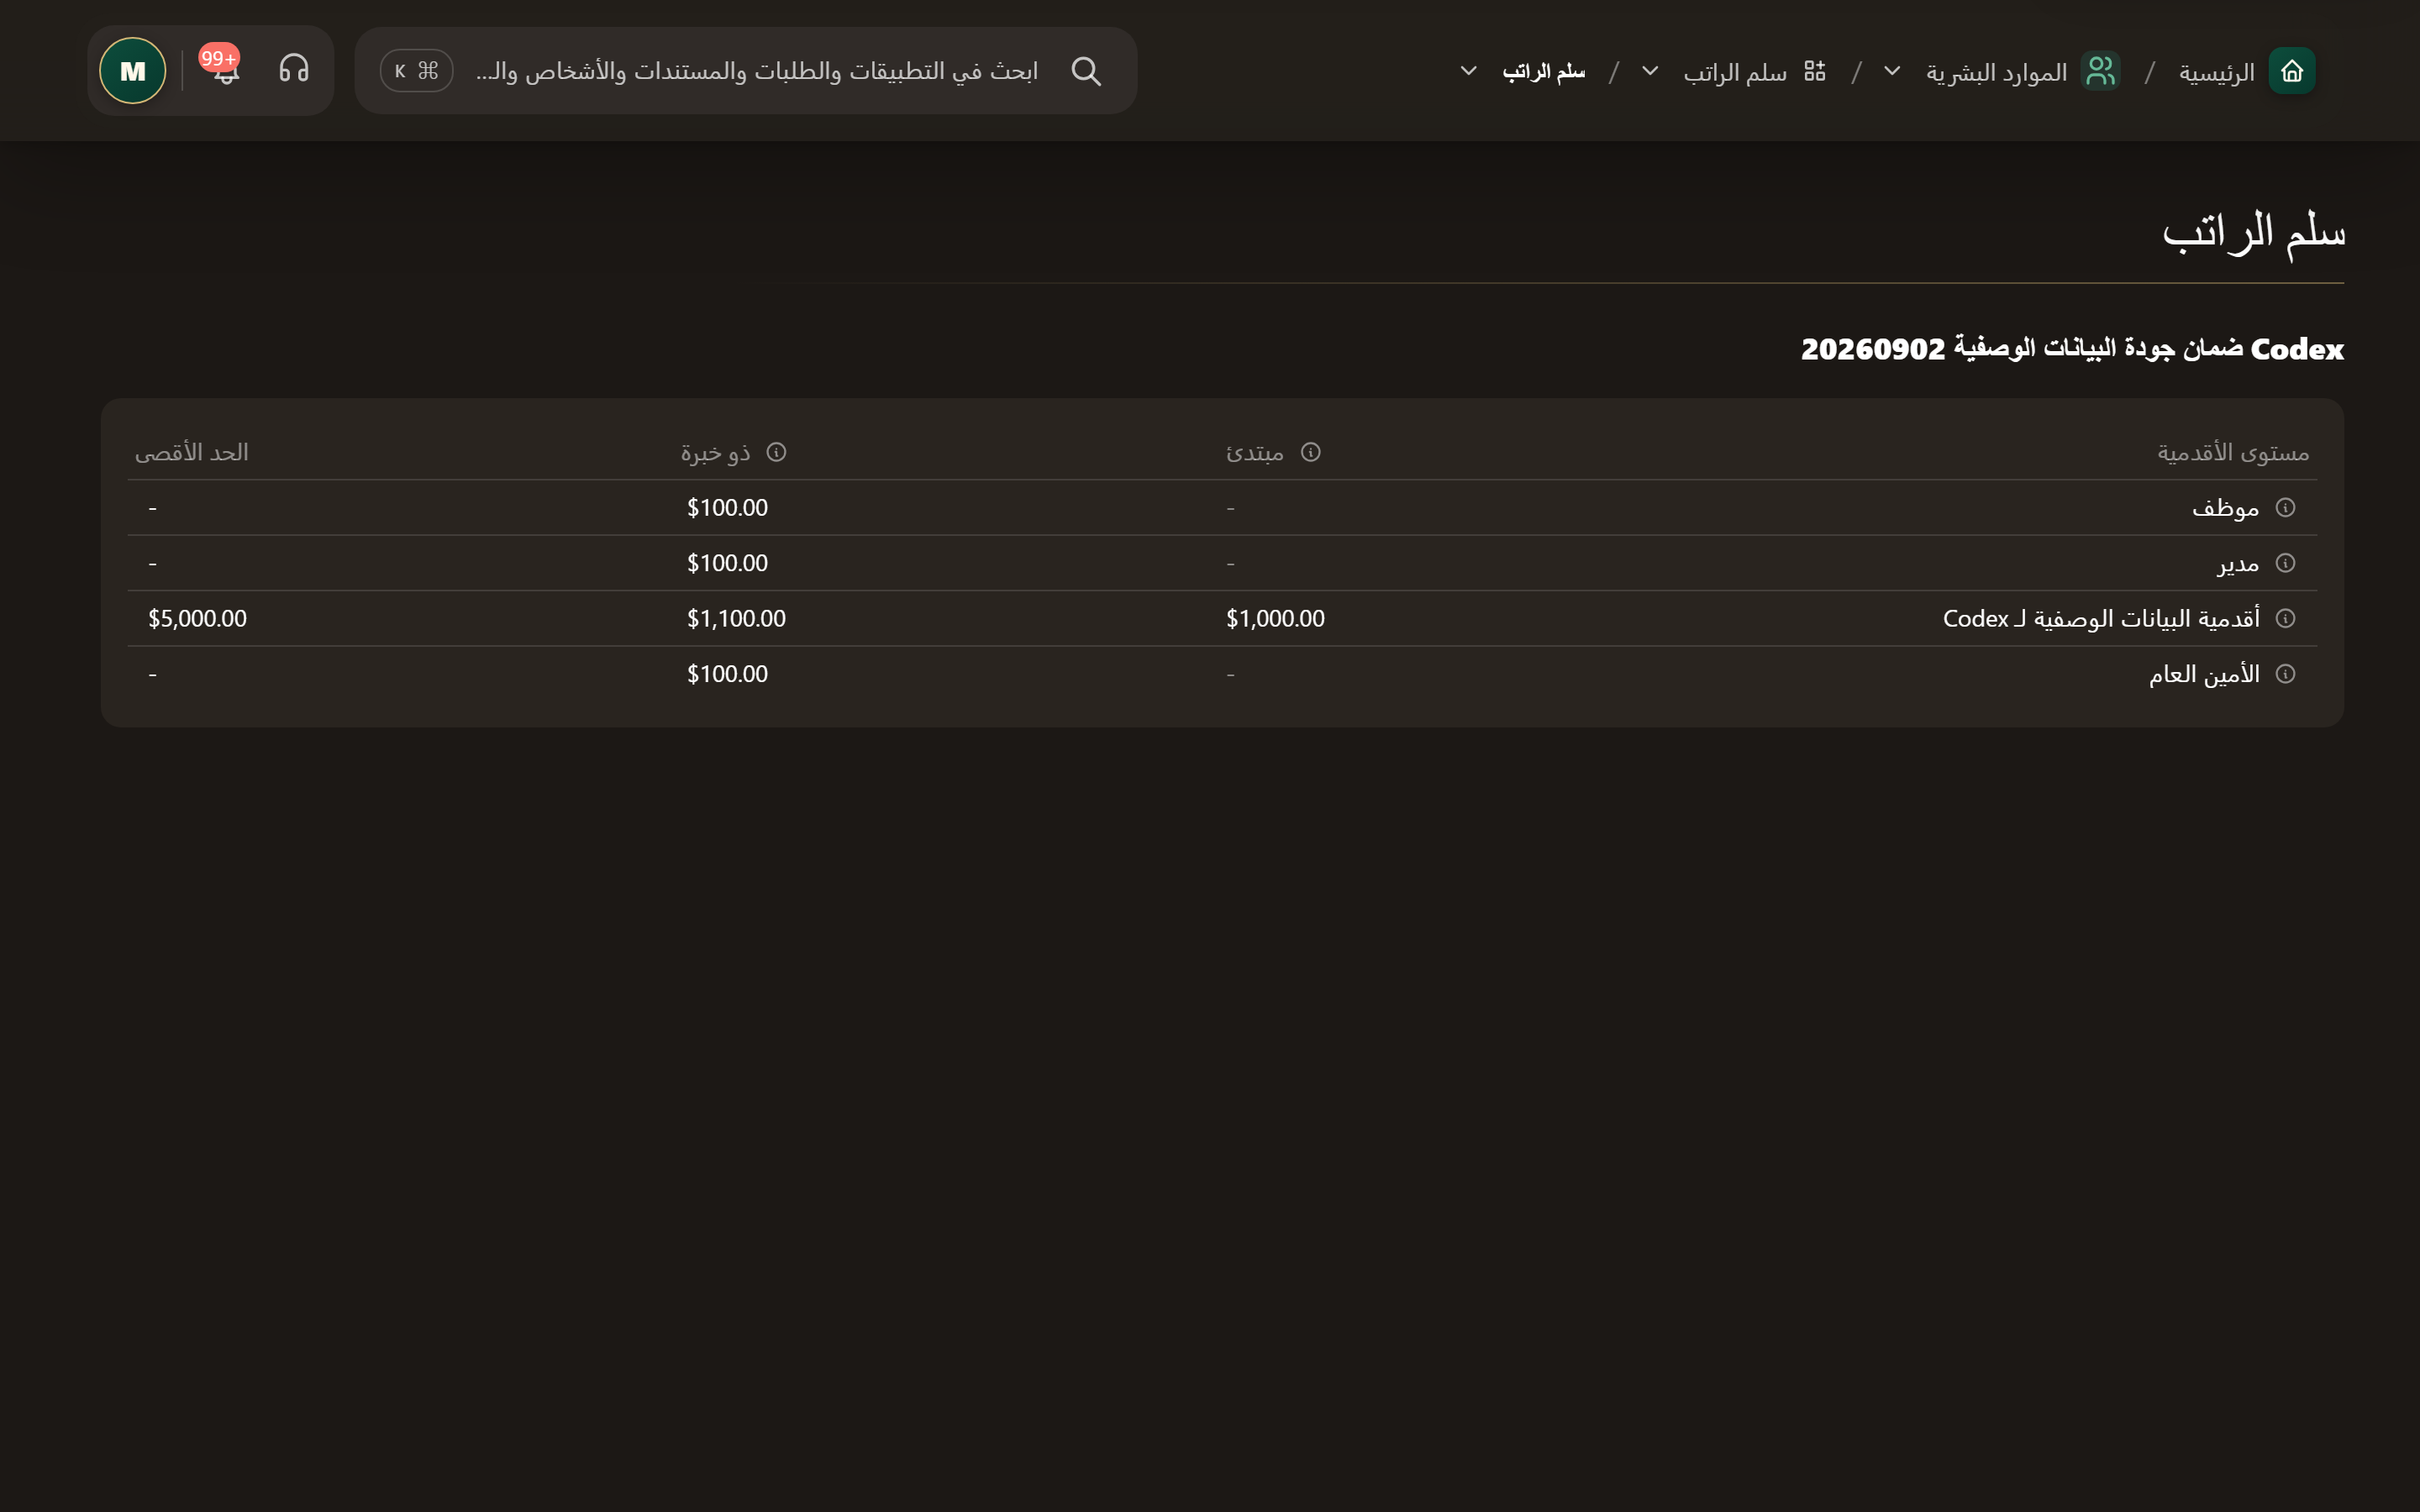
\includegraphics[width=0.95\linewidth]{figures/screens/ch03-feature-salary-scale-ar.png}
\caption{سلم الراتب: الصفحة كاملة في بيئة الاختبار}
\label{fig:hr-feature-salary-scale-screen}
\end{figure}

\begin{table}[H]
\centering
\caption{كيف تقرأ سلم الراتب؟}
\label{tab:hr-feature-salary-scale-data}
\rcZebra
\begin{tabularx}{\linewidth}{R{3.6cm} Y}
\rcHeaderRow
\thh{الجزء} & \thh{ماذا يعني؟}\\
جدول لكل مجموعة & كل مجموعة خبرة لها جدولها وعملتها.\\
الصفوف & المستويات الوظيفية، من الرتبة الأعلى إلى الأدنى.\\
الأعمدة & مستويات الخبرة بترتيبها، والعمود الأخير الحد الأقصى.\\
الخلية & الراتب المبدئي مع زيادات الخبرة حتى هذا المستوى \gen{}.\\
\end{tabularx}
\end{table}

لا يُعدَّل السلم مباشرة؛ غيّر المستويات الوظيفية أو مستويات الخبرة.

\begin{figure}[H]
\centering
\begin{tikzpicture}[node distance=0.4cm,stepBox/.append style={minimum width=6cm,text width=5.6cm,minimum height=0.7cm}]
  \node[stepBox] (s0) {\RL{مستويات الخبرة:}\\\RL{المجموعة والزيادات}};
  \node[stepBox,below=of s0] (s1) {\RL{المستويات الوظيفية:}\\\RL{الرواتب والرتب}};
  \node[stepBox,below=of s1] (s2) {\RL{سلم الراتب: راجع}\\\RL{الخلايا}};
  \node[stepBox,below=of s2] (s3) {\RL{التعيين: راجع الراتب}\\\RL{والعملة}};
  \draw[flowsTo] (s0) -- (s1);
  \draw[flowsTo] (s1) -- (s2);
  \draw[flowsTo] (s2) -- (s3);
\end{tikzpicture}
\rclegend
\caption{إن كانت مؤسستك تستخدم سلم الراتب}
\label{fig:hr-scale-setup}
\end{figure}

\subsection{جرّب وراجع}

\begin{enumerate}
  \item جهّز مجموعة الخبرة ومستوياتها، ثم المستويات الوظيفية. افتح «سلم الراتب».
  \item ابحث عن الدرجة ومستوى الخبرة وراجع الخلية. إن كانت غير متوقعة، افحص الراتب المبدئي والزيادة.
\end{enumerate}

\textbf{تحقق:} قارن المبلغ المرجعي براتب تعيين سارة وعملته. تبيّن الأسهم ترتيب الإعداد، ولا تعني دفع الراتب تلقائياً.

\clearpage
\section{مدخلات الرواتب}
\label{sec:hr-feature-payroll-inputs}

مدخل الراتب بند متغير لشهر محدد، مثل مكافأة أو خصم أو عمل إضافي، يُسجَّل على تعيين موظف.

\textbf{متى تفيد؟} كل مبلغ استثنائي مسجل وقابل للتتبع، بدلاً من تعديل الراتب يدوياً. \textbf{المسار:} «الموارد البشرية» / «الدفع» / «مدخلات الرواتب».

\begin{figure}[H]
\centering
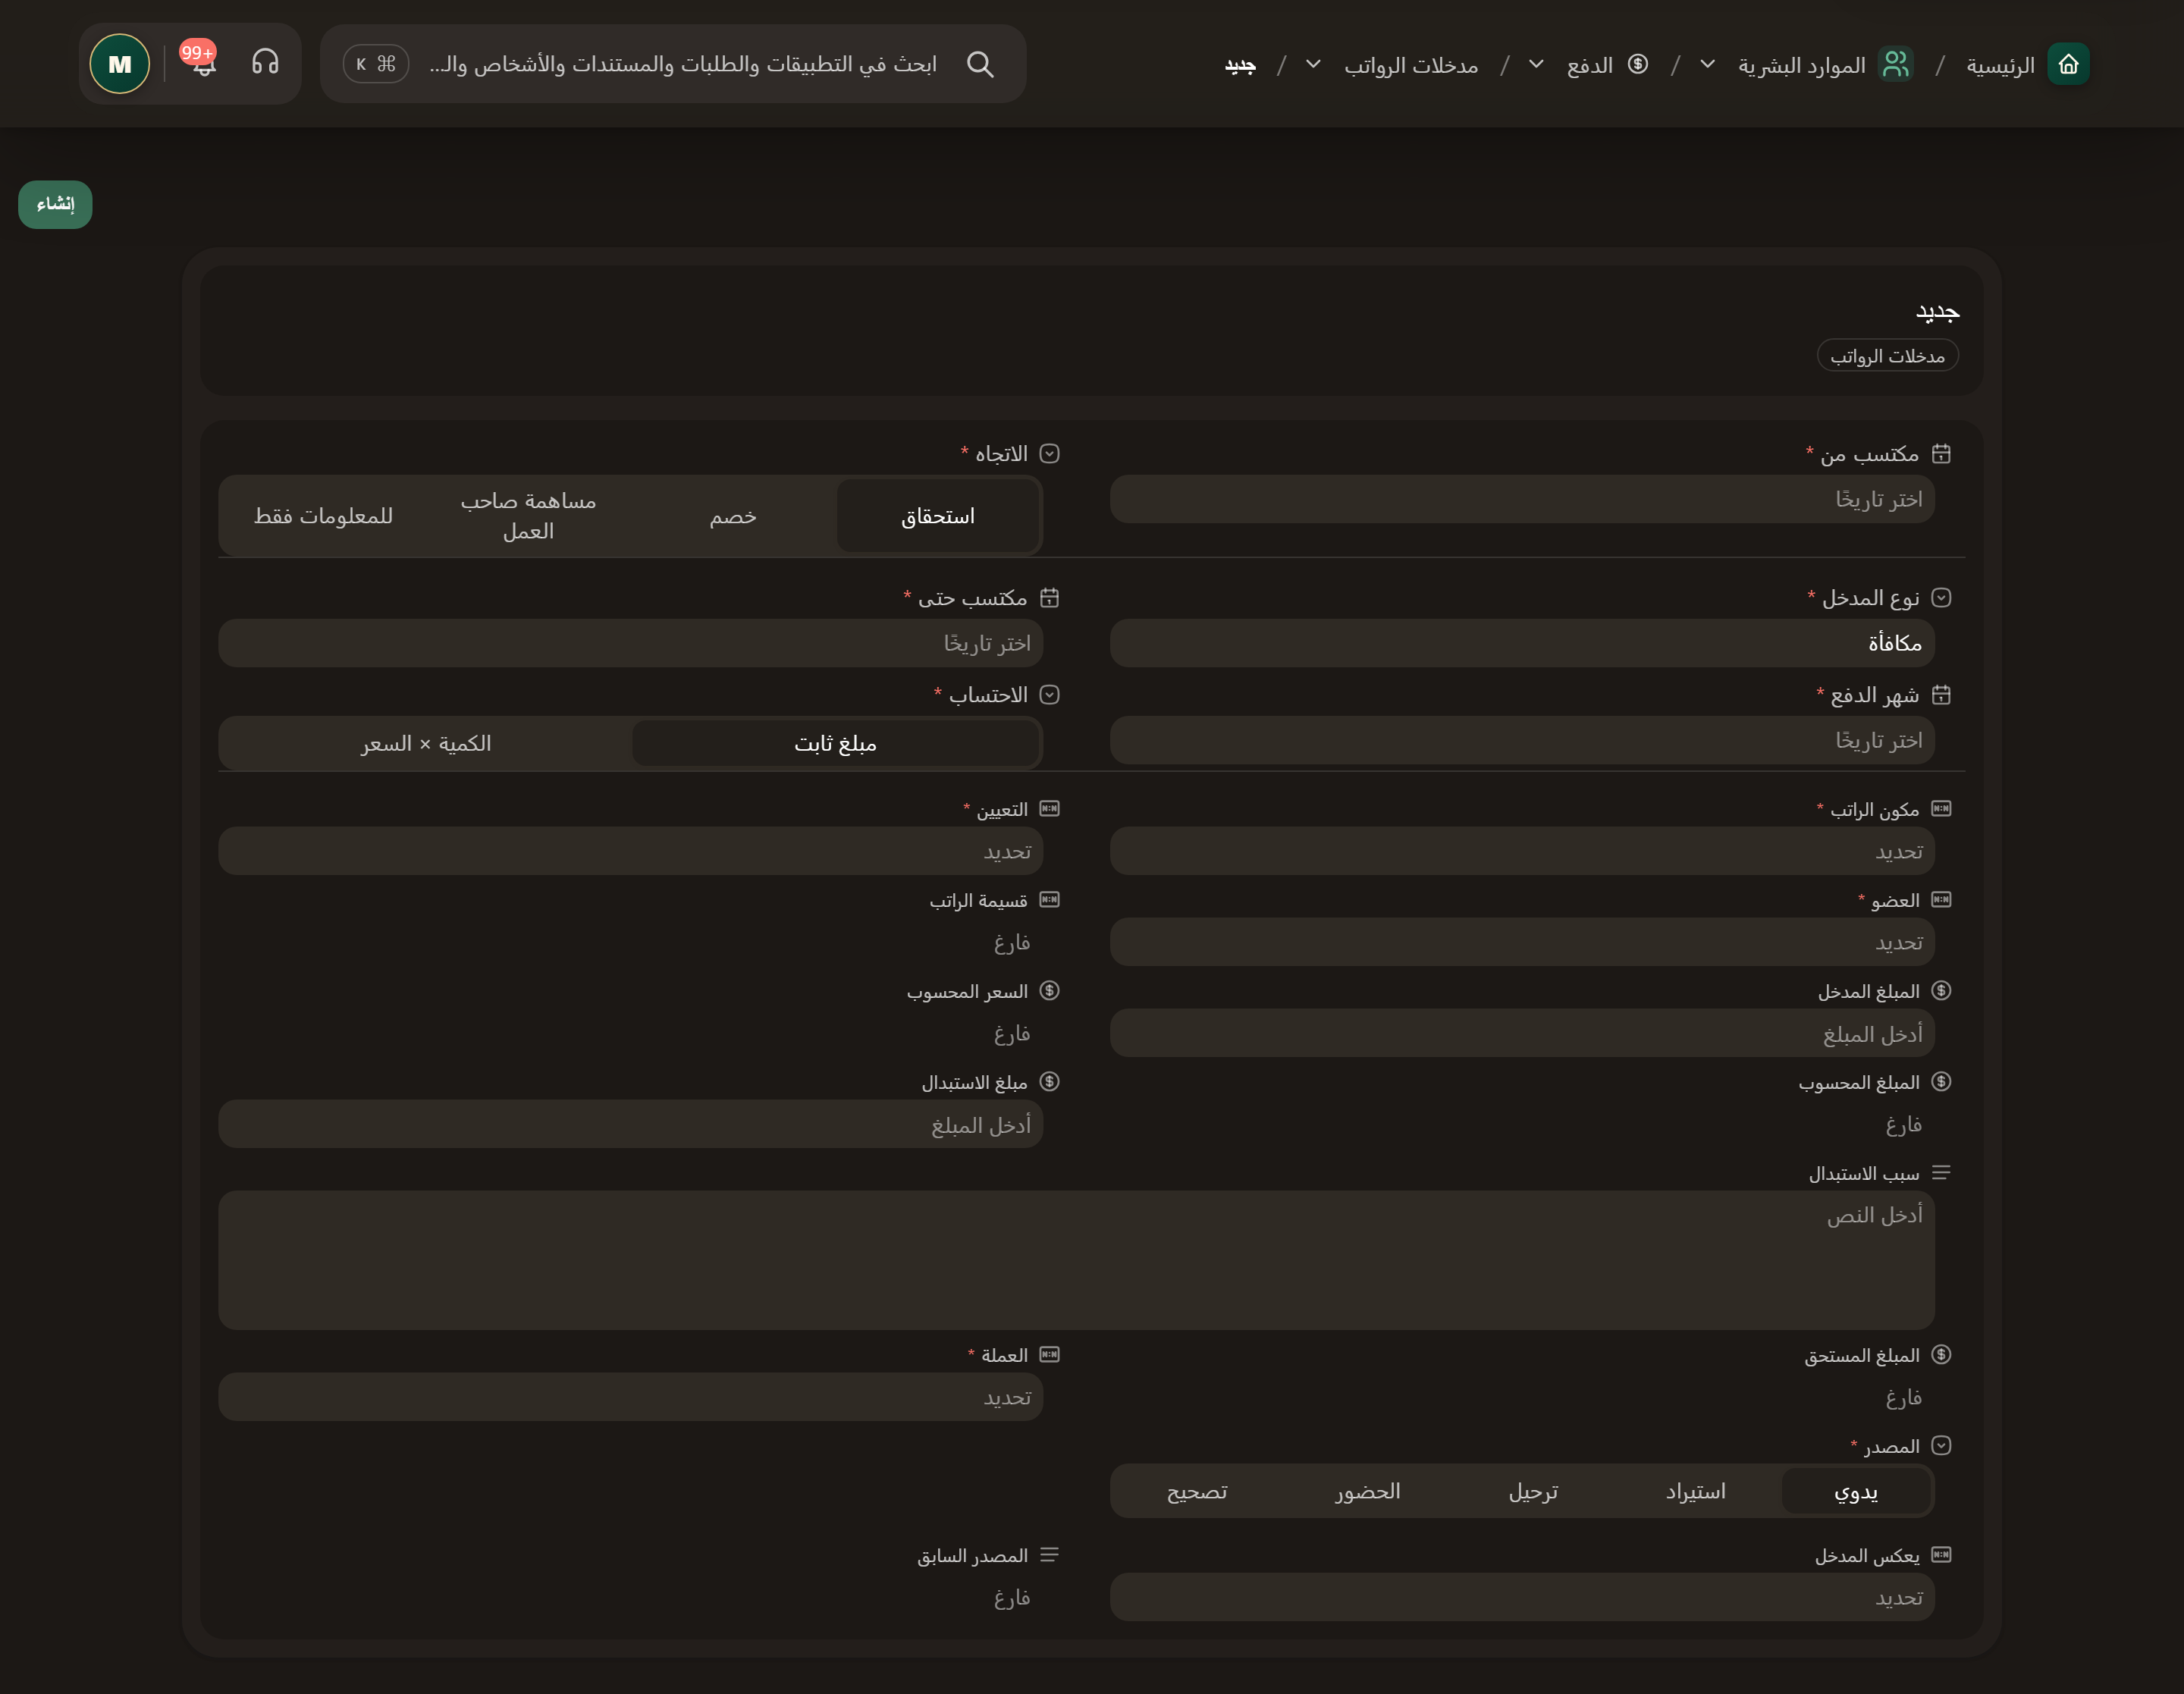
\includegraphics[width=0.95\linewidth]{figures/screens/ch03-payroll-input-fields-ar.png}
\caption{مدخلات الرواتب: أكمل الحقول المعلّمة بـ*؛ لم يُحفظ}
\label{fig:hr-feature-payroll-inputs-screen}
\end{figure}

\begin{table}[H]
\centering
\caption{ما الذي تسجله في مدخل الراتب؟}
\label{tab:hr-feature-payroll-inputs-data}
\rcZebra
\begin{tabularx}{\linewidth}{R{3.6cm} Y}
\rcHeaderRow
\thh{الحقل} & \thh{ما الذي تضيفه؟}\\
الاتجاه ونوع المدخل & \req{}: الاتجاه: استحقاق أو خصم أو مساهمة صاحب العمل أو للمعلومات فقط؛ النوع: مكافأة، خصم، عمل إضافي، رد مصروف، تسوية.\\
المكون والتعيين والعضو & \req{}: مكون الراتب، والعضو وتعيينه.\\
الفترة & مكتسب من وحتى، وشهر الدفع \req{}.\\
الاحتساب & مبلغ ثابت، أو الكمية × السعر؛ وفي العمل الإضافي: الساعات وتصنيف الوقت: نهاري، ليلي، يوم الراحة، العطلة.\\
الاستبدال & مبلغ بديل يحل محل المحسوب، وسببه \opt{}.\\
النتيجة & السعر والمبلغ المحسوب والمبلغ المستحق وتفاصيل الاحتساب \gen{}.\\
\end{tabularx}
\end{table}

\subsection{ما الذي يمكنك فعله؟}

\begin{itemize}
  \item «معاينة الاحتساب» تحسب المبلغ من سياسة الرواتب وشروط التعويض.
  \item يُقفل المدخل عند اعتماد قسيمة تستخدمه. للتصحيح بعدها أضف مدخلاً جديداً واختر المدخل الأصلي في «يعكس المدخل».
\end{itemize}

\begin{figure}[H]
\centering
\begin{tikzpicture}[node distance=0.5cm,stepBox/.append style={minimum width=6.5cm,text width=6.1cm,minimum height=0.8cm}]
  \node[stepBox] (a) {\RL{تسجيل البند المعتمد}};
  \node[stepBox,below=of a] (b) {\RL{معاينة حسابه}};
  \node[stepBox,below=of b] (c) {\RL{مراجعة قسيمة الراتب}};
  \draw[flowsTo] (a) -- (b);
  \draw[flowsTo] (b) -- (c);
\end{tikzpicture}
\rclegend
\caption{خطوات الاستخدام؛ الأسهم لا تعني معالجة تلقائية}
\label{fig:hr-feature-payroll-inputs-flow}
\end{figure}

\subsection{جرّب وراجع}

\begin{enumerate}
  \item بعد مراجعة الوقت والإجازات، افتح «مدخلات الرواتب» وابحث عن البند لتجنب تكراره.
  \item أضف: «استحقاق»، «مكافأة»، المكون، تعيين سارة، الفترة وشهر الدفع، «مبلغ ثابت» والمبلغ المعتمد. احفظ.
  \item افتح «معاينة الاحتساب» وراجع المبلغ المستحق.
\end{enumerate}

\textbf{تحقق:} يظهر المبلغ في قسيمة سارة بعد «احتساب». المعاينة ليست دفعاً.

\clearpage
\section{قسائم الرواتب}
\label{sec:hr-feature-salary-slips}

قسيمة الراتب حساب راتب موظف لفترة: أيامه ومستحقاته وخصوماته وصافي راتبه. وحالاتها: مسودة، محسوبة، معتمدة.

\textbf{متى تفيد؟} راجع حساب سارة الفردي قبل إعداد كشف الرواتب، لتتبّع كل مبلغ إلى بنده. \textbf{المسار:} «الموارد البشرية» / «الدفع» / «قسائم الرواتب».

\begin{figure}[H]
\centering
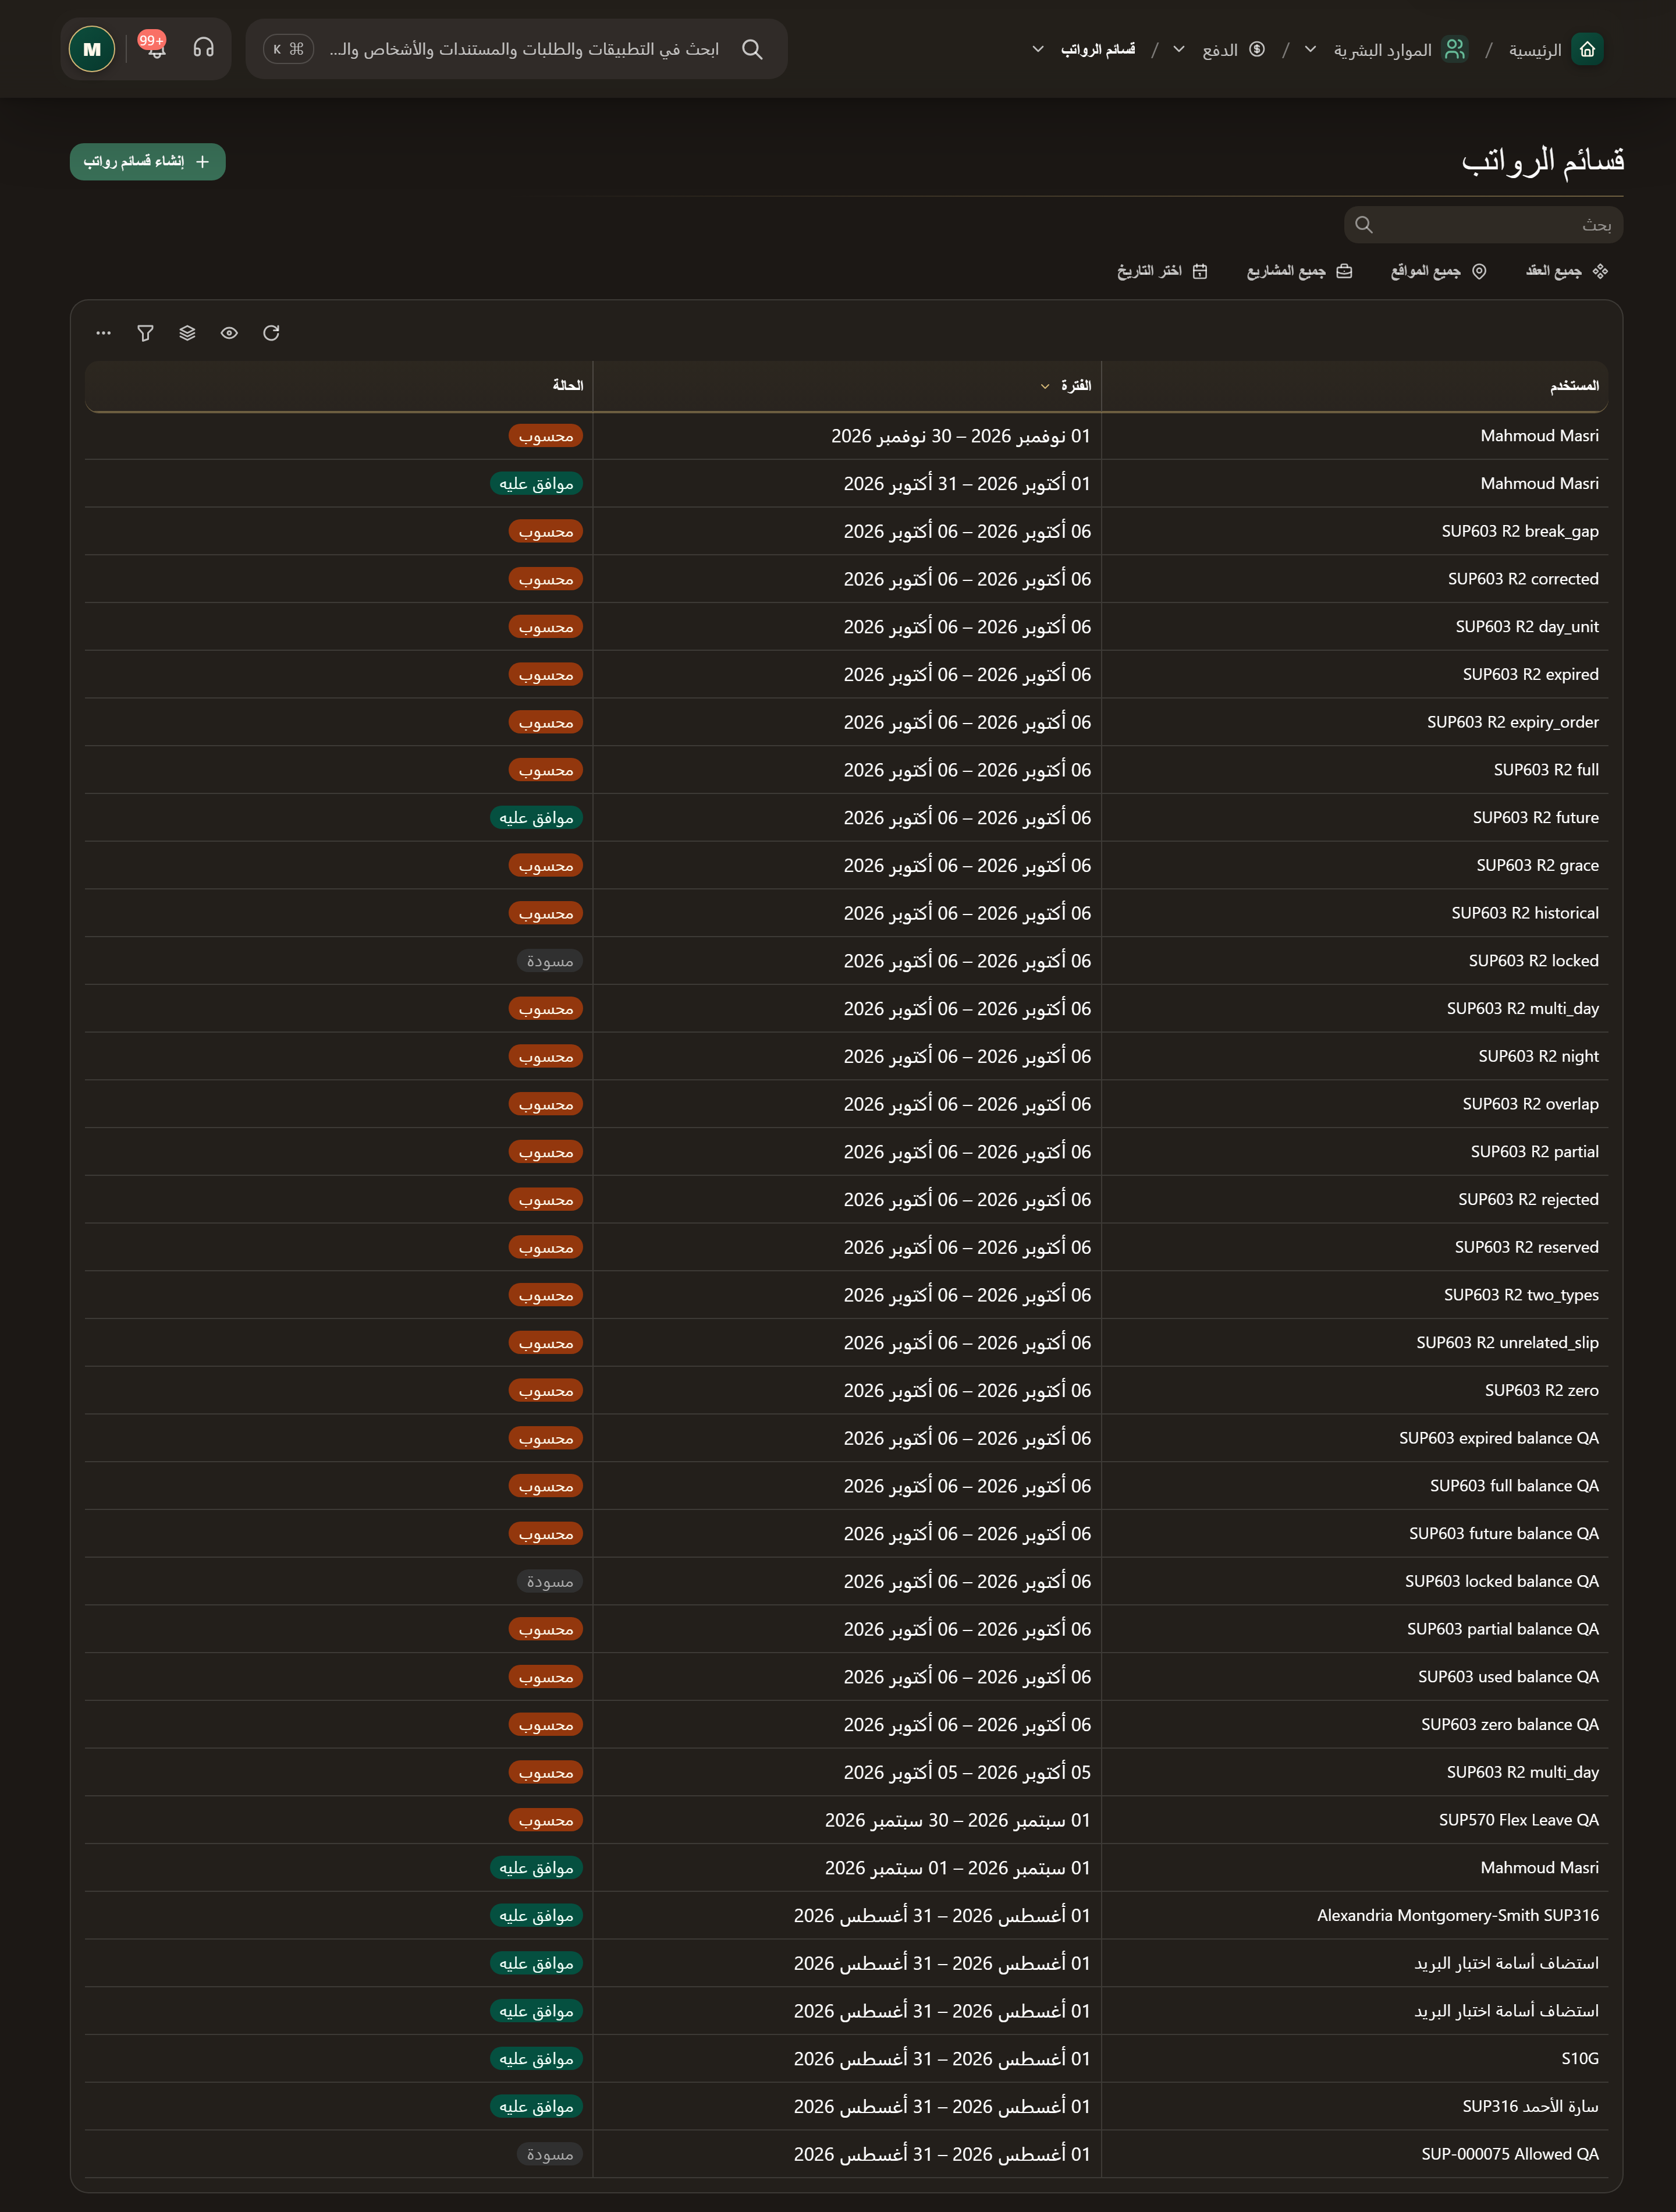
\includegraphics[width=0.95\linewidth]{figures/screens/ch03-create-slips-clear-ar.png}
\caption{قسائم الرواتب: الصفحة كاملة قبل إنشاء القسائم}
\label{fig:hr-feature-salary-slips-screen}
\end{figure}

\begin{table}[H]
\centering
\caption{ما الذي تعرضه القسيمة؟}
\label{tab:hr-feature-salary-slips-data}
\rcZebra
\begin{tabularx}{\linewidth}{R{3.6cm} Y}
\rcHeaderRow
\thh{القسم} & \thh{ماذا يعرض؟}\\
معلومات الموظف & الاسم والمنصب والموقع وبداية العقد ونهايته.\\
ملخص الدفع & الفترة، أيام العمل، العملة، الراتب الأساسي للفترة.\\
الأيام & أيام العمل والعطل والإجازات المدفوعة وغير المدفوعة والعمل الإضافي.\\
حساب الراتب & بند لكل مصدر بمعادلته، ثم المبلغ المستحق والتقريب وإجمالي الراتب الصافي.\\
المشاريع والملاحظات & نسبة كل مشروع ومبلغه، وملاحظات القسيمة.\\
\end{tabularx}
\end{table}

\begin{itemize}
  \item التصفية بالاسم والوحدات والمواقع والمشاريع والشهر.
  \item «احتساب» ثم «إعادة الاحتساب»، و«اعتماد»، و«حذف» القسيمة المسودة أو المحسوبة. القسيمة المعتمدة لا تُعدّل.
\end{itemize}

\begin{figure}[H]
\centering
\begin{tikzpicture}[node distance=0.4cm,stepBox/.append style={minimum width=6.5cm,text width=6.1cm,minimum height=0.7cm}]
  \node[stepBox] (m0) {\RL{التعيين وبيانات}\\\RL{الموظف}};
  \node[stepBox,below=of m0] (m1) {\RL{مراجعة الدوام}\\\RL{والإجازات}};
  \node[stepBox,below=of m1] (m2) {\RL{مراجعة مدخلات}\\\RL{الرواتب}};
  \node[stepBox,below=of m2] (m3) {\RL{احتساب قسيمة الراتب}\\\RL{واعتمادها}};
  \node[stepBox,below=of m3] (m4) {\RL{توليد كشف الرواتب}\\\RL{ومراجعته}};
  \draw[flowsTo] (m0) -- (m1);
  \draw[flowsTo] (m1) -- (m2);
  \draw[flowsTo] (m2) -- (m3);
  \draw[flowsTo] (m3) -- (m4);
\end{tikzpicture}
\rclegend
\caption{مسار المراجعة من الموظف إلى كشف الرواتب}
\label{fig:hr-review-flow}
\end{figure}

\subsection{جرّب وراجع}

\begin{enumerate}
  \item افتح «قسائم الرواتب»، ثم «إنشاء قسائم رواتب».
  \item اختر «نهاية الفترة»، ثم حدّد صفّ سارة ومنصبها. راجع «بداية الفترة»؛ تبدأ أول قسيمة من تاريخ بدء التعيين، ويمكنك تعديل التاريخ.
  \item أنشئ المسودة بالزر الذي يعرض عدد المحددين، ثم افتح قسيمتها. إن وُجدت مسودة، راجعها أو احذفها بدلاً من إنشاء نسخة مكررة.
  \item اختر «احتساب». راجع الأيام والبنود والصافي. بعد تغيير المدخلات اختر «إعادة الاحتساب».
  \item عند صحة البنود اختر «اعتماد» وأكّد. الاعتماد يُقفل مدخلات الرواتب المستخدمة فيها.
\end{enumerate}

\textbf{تحقق:} تظهر حالة القسيمة «معتمد» في القائمة. الاعتماد لا يعني أن الراتب دُفع.

\clearpage
\section{كشوف الرواتب}
\label{sec:hr-feature-payrolls}

كشف الرواتب يجمع القسائم المعتمدة لشهر في كشف واحد، بإجمالي لكل عضو ولكل مشروع.

\textbf{متى تفيد؟} بعد فحص القسائم، لمراجعة رواتب الشهر واعتمادها وتصديرها. \textbf{المسار:} «الموارد البشرية» / «الدفع» / «كشوف الرواتب».

\begin{figure}[H]
\centering
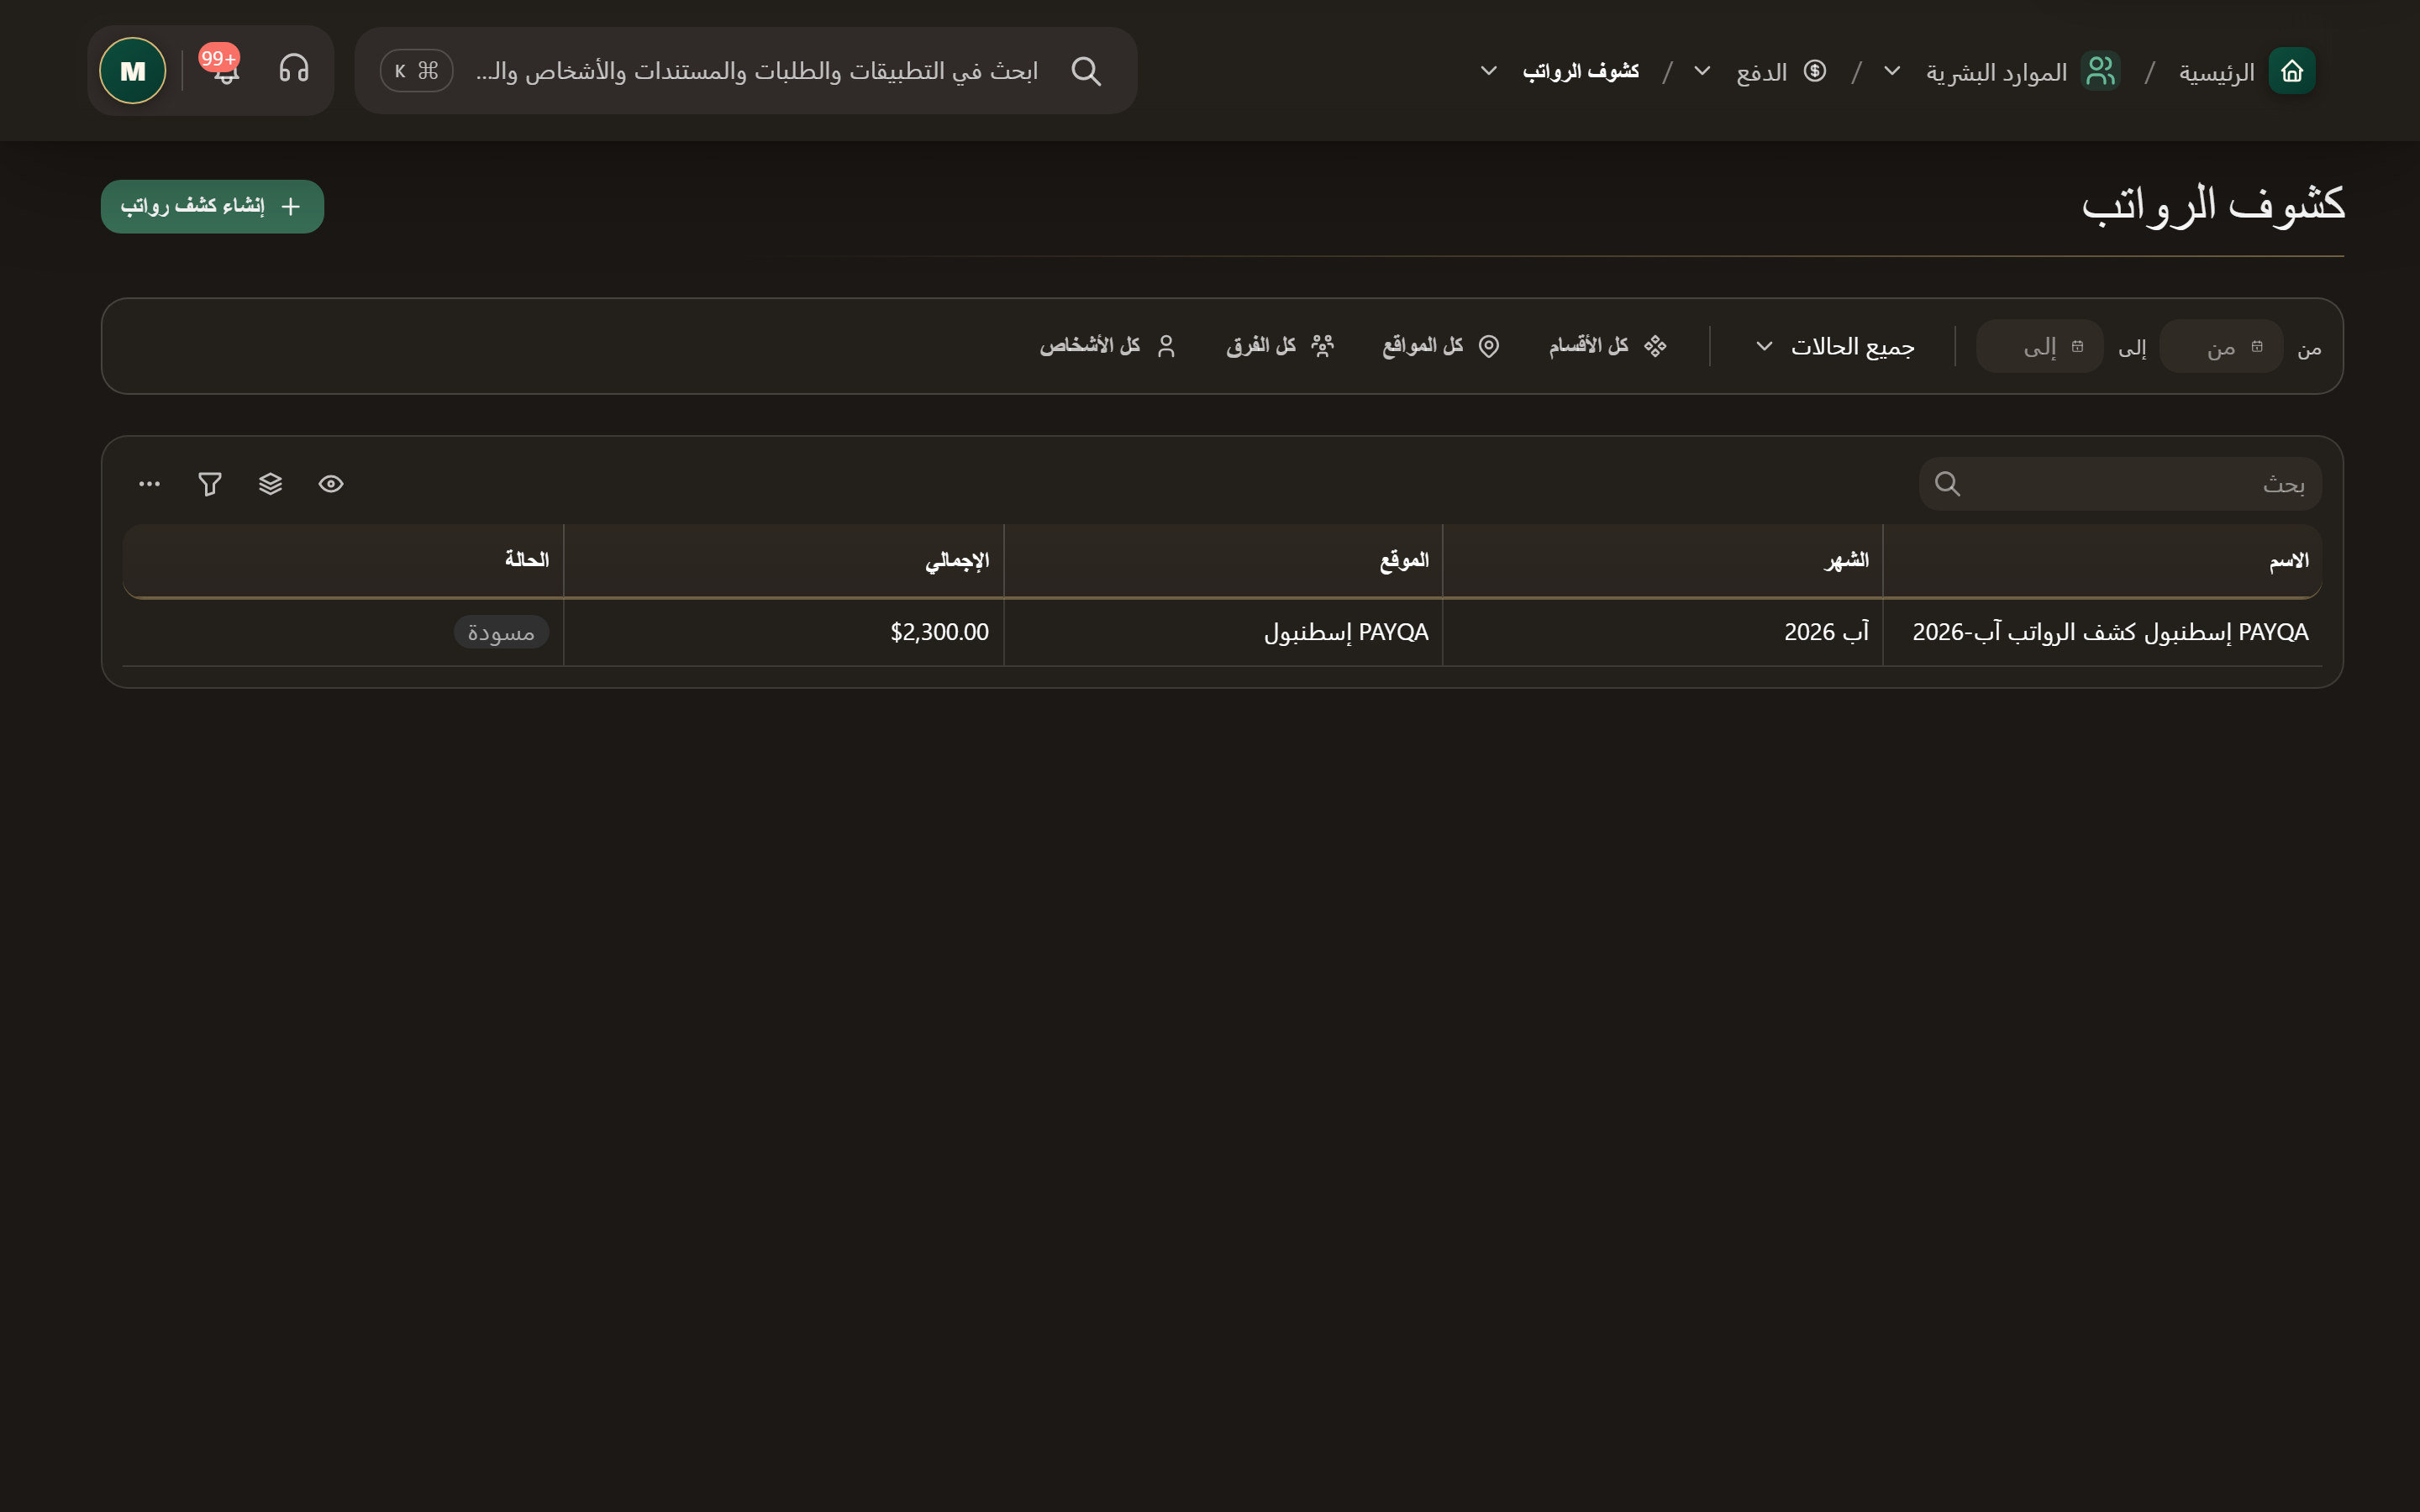
\includegraphics[width=0.95\linewidth]{figures/screens/ch03-feature-payrolls-ar.png}
\caption{كشوف الرواتب: الصفحة كاملة في بيئة الاختبار}
\label{fig:hr-feature-payrolls-screen}
\end{figure}

\begin{table}[H]
\centering
\caption{ما الذي يضمه كشف الرواتب؟}
\label{tab:hr-feature-payrolls-data}
\rcZebra
\begin{tabularx}{\linewidth}{R{3.6cm} Y}
\rcHeaderRow
\thh{الجزء} & \thh{ماذا يعرض؟}\\
الإنشاء & الشهر والسنة؛ المصدر: القسائم المعتمدة أو جميع الأعضاء؛ والتصفية بالأقسام والمواقع والفرق والأشخاص.\\
القائمة & الاسم والشهر والموقع والإجمالي والحالة: مسودة أو معتمد.\\
المدفوعات & لكل عضو أو لكل مشروع: أيام العمل، المكافآت، الخصومات، الصافي، المبلغ المستحق، الملاحظات.\\
المشاريع & نسبة كل مشروع ومبلغه، وإجمالي لكل عملة.\\
\end{tabularx}
\end{table}

\begin{itemize}
  \item «تصدير \en{PDF}» لتقرير الكشف، مسودةً أو معتمداً.
  \item «اعتماد كشف الرواتب» لا يمكن التراجع عنه.
\end{itemize}

\begin{figure}[H]
\centering
\begin{tikzpicture}[node distance=0.5cm,stepBox/.append style={minimum width=6.5cm,text width=6.1cm,minimum height=0.8cm}]
  \node[stepBox] (a) {\RL{مراجعة القسائم}\\\RL{المعتمدة}};
  \node[stepBox,below=of a] (b) {\RL{توليد كشف الشهر}};
  \node[stepBox,below=of b] (c) {\RL{فحص الإجماليات}\\\RL{واعتماد الكشف}};
  \draw[flowsTo] (a) -- (b);
  \draw[flowsTo] (b) -- (c);
\end{tikzpicture}
\rclegend
\caption{خطوات الاستخدام؛ الأسهم لا تعني معالجة تلقائية}
\label{fig:hr-feature-payrolls-flow}
\end{figure}

\subsection{جرّب وراجع}

\begin{enumerate}
  \item افتح «كشوف الرواتب»، ثم «إنشاء كشف رواتب». اختر الشهر والسنة و«قسائم الرواتب المعتمدة».
  \item حدد الموظفين واختر «توليد». إن ظهر أن الأعضاء موجودون في كشف آخر، اختر «إلغاء تحديد الأعضاء».
  \item افتح الكشف وراجع الأشخاص والإجمالي، ثم «اعتماد كشف الرواتب».
\end{enumerate}

\textbf{تحقق:} تتبع كل مبلغ إلى قسيمته. إن غاب موظف، راجع الشهر والتصفية وحالة قسيمته.

\begin{rcwarn}[الحساب ليس دفعاً]
اعتماد الكشف يغيّر حالته فقط. تحقق من التحويل وسجلات الدفع وفق إجراءات مؤسستك.
\end{rcwarn}
